% Copyright (c) 2022 by Lars Spreng
% This work is licensed under the Creative Commons Attribution 4.0 International License. 
% To view a copy of this license, visit http://creativecommons.org/licenses/by/4.0/ or send a letter to Creative Commons, PO Box 1866, Mountain View, CA 94042, USA.

%~~~~~~~~~~~~~~~~~~~~~~~~~~~~~~~~~~~~~~~~~~~~~~~~~~~~~~~~~~~~~~~~~~~~~~~~~~~~~~
% You can add your packages and commands to the loadslides.tex file. 
% The files in the folder "styles" can be modified to change the layout and design of your slides.
% I have included examples on how to use the template below. 
% Some of it these examples are taken from the Metropolis template.
%~~~~~~~~~~~~~~~~~~~~~~~~~~~~~~~~~~~~~~~~~~~~~~~~~~~~~~~~~~~~~~~~~~~~~~~~~~~~~~



\documentclass[
11pt,notheorems,hyperref={pdfauthor=whatever}
]{beamer}
\usepackage{float}
\usepackage[center]{subfigure}
\usepackage{microtype}
\usepackage{graphicx}
\usepackage{amsmath}
\usepackage{amssymb}
\usepackage{mathtools}
\usepackage{amsthm}


% Copyright (c) 2022 by Lars Spreng
% This work is licensed under the Creative Commons Attribution 4.0 International License. 
% To view a copy of this license, visit http://creativecommons.org/licenses/by/4.0/ or send a letter to Creative Commons, PO Box 1866, Mountain View, CA 94042, USA.

%~~~~~~~~~~~~~~~~~~~~~~~~~~~~~~~~~~~~~~~~~~~~~~~~~~~~~~~~~~~~~~~~~~~~~~~~~~~~~~
% Add your packages and commands to this file
%~~~~~~~~~~~~~~~~~~~~~~~~~~~~~~~~~~~~~~~~~~~~~~~~~~~~~~~~~~~~~~~~~~~~~~~~~~~~~~

%~~~~~~~~~~~~~~~~~~~~~~~~~~~~~~~~~~~~~~~~~~~~~~~~~~~~~~~~~~~~~~~~~~~~~~~~~~~~~~
\RequirePackage{palatino}
\RequirePackage[utf8]{inputenc}
\RequirePackage[T1]{fontenc}

\usefonttheme{serif}

\usepackage{styles/elegantmacros}
\usefolder{styles}
\usetheme[style=blue]{elegant}

\newcommand{\makepart}[1]{ % For convenience
  \part{#1} \frame{\partpage}
}

%~~~~~~~~~~~~~~~~~~~~~~~~~~~~~~~~~~~~~~~~~~~~~~~~~~~~~~~~~~~~~~~~~~~~~~~~~~~~~~
\RequirePackage{pgfplots}

%~~~~~~~~~~~~~~~~~~~~~~~~~~~~~~~~~~~~~~~~~~~~~~~~~~~~~~~~~~~~~~~~~~~~~~~~~~~~~~
% Figures
\RequirePackage{booktabs}
\RequirePackage{colortbl}
\RequirePackage{ragged2e}
\RequirePackage{schemabloc}
%\RequirePackage{natbib}coloneqq
\usepackage[square,numbers]{natbib}
\RequirePackage{caption}
\RequirePackage{subcaption}
\RequirePackage{tabularx}
\RequirePackage{array}
\RequirePackage{multirow}
\RequirePackage{algorithm2e}
\RequirePackage{algorithmic}
\RequirePackage{animate}
% \usepackage[
%   style=authoryear,
% ]{biblatex}
% \addbibresource{references.bib}
\newcolumntype{Y}{>{\centering\arraybackslash}X}
\usepackage{url}
\usepackage{forest}
%~~~~~~~~~~~~~~~~~~~~~~~~~~~~~~~~~~~~~~~~~~~~~~~~~~~~~~~~~~~~~~~~~~~~~~~~~~~~~~

%~~~~~~~~~~~~~~~~~~~~~~~~~~~~~~~~~~~~~~~~~~~~~~~~~~~~~~~~~~~~~~~~~~~~~~~~~~~~~~
% Figures
\RequirePackage{wrapfig}
% \RequirePackage{pgfplots}
\RequirePackage{graphicx}
\RequirePackage{adjustbox}
\RequirePackage{environ}
% \pgfplotsset{compat=1.18}

\makeatletter
\newsavebox{\measure@tikzpicture}
\NewEnviron{scaletikzpicturetowidth}[1]{%
  \def\tikz@width{#1}%
  \def\tikzscale{1}\begin{lrbox}{\measure@tikzpicture}%
    \BODY
  \end{lrbox}%
  \pgfmathparse{#1/\wd\measure@tikzpicture}%
  \edef\tikzscale{\pgfmathresult}%
  \BODY
}
\makeatother
%~~~~~~~~~~~~~~~~~~~~~~~~~~~~~~~~~~~~~~~~~~~~~~~~~~~~~~~~~~~~~~~~~~~~~~~~~~~~~~

%~~~~~~~~~~~~~~~~~~~~~~~~~~~~~~~~~~~~~~~~~~~~~~~~~~~~~~~~~~~~~~~~~~~~~~~~~~~~~~
% Maths 
\RequirePackage{textcomp}
\RequirePackage{amsmath}
\RequirePackage{amsthm}
\RequirePackage{mathtools}
%\RequirePackage{bbm}
%\RequirePackage{algorithm}
%\RequirePackage[osf,sc]{mathpazo}
%\RequirePackage{pifont}
%\newcommand{\xmark}{\ding{55}}%
%\numberwithin{equation}{section}
\DeclareMathOperator*{\argmax}{arg\,max}
\DeclareMathOperator*{\argmin}{arg\,min}

\setbeamertemplate{theorems}[numbered] % to number

\theoremstyle{definition}
\newtheorem{fact}{Fact}[section]
\newtheorem{examp}{Example}[section]

\theoremstyle{plain}
\newtheorem{definition}{Definition}[section]
\newtheorem{proposition}{Proposition}
\newtheorem{theorem}{Theorem}
\newtheorem{assumption}{Assumption}

\providecommand{\H}{\mathscr{H}}
\providecommand{\E}{\mathbb{E}}
\makeatletter
\def\munderbar#1{\underline{\sbox\tw@{$#1$}\dp\tw@\z@\box\tw@}}
\makeatother

%~~~~~~~~~~~~~~~~~~~~~~~~~~~~~~~~~~~~~~~~~~~~~~~~~~~~~~~~~~~~~~~~~~~~~~~~~~~~~~
 % Loads packages and some defined commands

\title[
Introduction to Deep Learning: Excutive Master - IASD
]{Dive into Deep Learning: A Comprehensive Introduction}

\subtitle{From AI Fundamentals to Cutting-Edge Deep Learning Techniques}

\author[
Alexandre V\'erine
]{
    Alexandre Vérine,\\
    Research Fellow, ENS-PSL\\
    Universit\'e PSL\\
    \url{www.alexverine.com}
}

\institute{
Executive Master IASD\\
    Universit\'e Paris-Dauphine, PSL}
\date{\today}

\begin{document}

% Generate title page
{
\setbeamertemplate{footline}{}
\begin{frame}
    \titlepage
\end{frame}


\begin{frame}{Outline}
    Schedule :
    \begin{itemize}
        \item Monday 13th of October Evenning : From Fundamentals to Deep Learning + TP1 Introduction to PyTorch and basic Neural Networks
        \item Tuesday 14th of October Morning : End of TP1, CNNs and applications
        \item Tuesday 14th of October Afternoon : Deep Learning in Action: From Neural Networks to Transformer Models + TP 2 Train an Autoencoder.
        \item Tuesday 13th of January Morning : Techniques to Improve Deep Learning Training, + TP3 Image Segmentation with U-Net
        \item Tuesday 13th of January Afternoon : TP 4 Generative Adversarial Networks
    \end{itemize}
\end{frame}



}
\addtocounter{framenumber}{-2}

% You can declare different parts as a parentof sections
\begin{frame}{AI 101: From Fundamentals to Deep Learning}
    \tableofcontents[part=1]
\end{frame}
\begin{frame}{Deep Learning in Action: From Neural Networks to Transformer Models}
    \tableofcontents[part=2]
\end{frame}
\begin{frame}{Techniques to Improve Deep Learning Training}
    \tableofcontents[part=3]
\end{frame}

% \begin{frame}{Deep Learning and Applications}
%     \tableofcontents[part=4]
% \end{frame}

\begin{frame}{Your turn: Hands-on Deep Learning}
    \tableofcontents[part=4]
\end{frame}




\makepart{AI 101: From Fundamentals to Deep Learning}

\section{Introduction to Artificial Intelligence}
\subsection{Deep Learning in the AI family}


\begin{frame}{}
	\begin{columns}[T,onlytextwidth]
		\column{0.4\textwidth}
		In general, among all the class of AI algorithms, we make the difference between 3 sub-categories :
		\begin{itemize}
			\item \alert{Artificial Intelligence} : human designed program and...
			\item \alert{Machine Learning} : human designed features with learned mapping such as Support Vector Machine, Kernels methods, Logistic Regression and ...
			\item \alert{Deep Learning: } Learned features with learned mapping such as Multilayer Perceptron, Convolutional Networks, ...
		\end{itemize}

		\column{0.6\textwidth}
		\begin{figure}
			\centering
			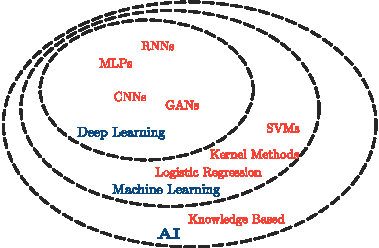
\includegraphics[width=0.9\textwidth]{figures/IAMLDL.pdf}
			\caption{Subsets of Artificial Intelligence}
		\end{figure}
	\end{columns}
\end{frame}

\begin{frame}{}

	\begin{columns}[T,onlytextwidth]
		\column{0.7\textwidth}
		In the field of Artificial Intelligence, the fundamental objective is to find a function $f$ that can perform a desired task. This function can either be set by a human or can be learned through training. \newline

		For example, in the context of a binary classification task, the goal is to determine $f(x)$ such that $f(x) = 0$ when the label of $x$ is 0 and $f(x) = 1$ when its label is 1. The choice of AI model impacts the expressivity of the function $f$. \newline

		For example, a logistic regression model uses a linear function to make decisions, where $f(x) = \mathrm{sgn}(Ax+b)$. The expressivity of the model can be increased by using more complex functions, such as polynomials or radial basis functions.
		\column{0.25\textwidth}
		\begin{figure}
			\centering
			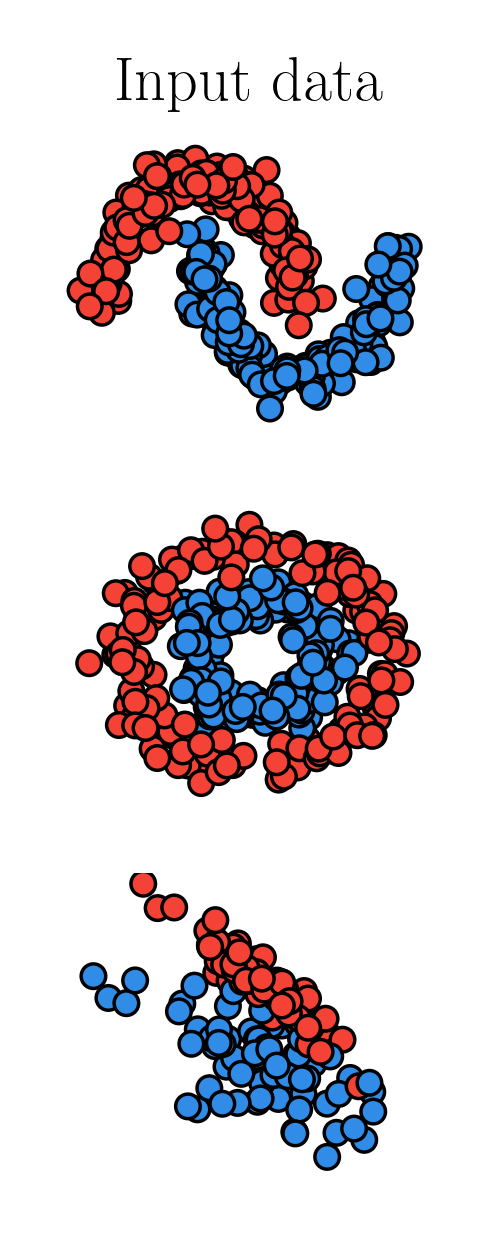
\includegraphics[width=0.7\textwidth]{figures/2Ddata.png}
		\end{figure}
	\end{columns}

\end{frame}

\begin{frame}{}{Classification task}
	\begin{figure}
		\centering
		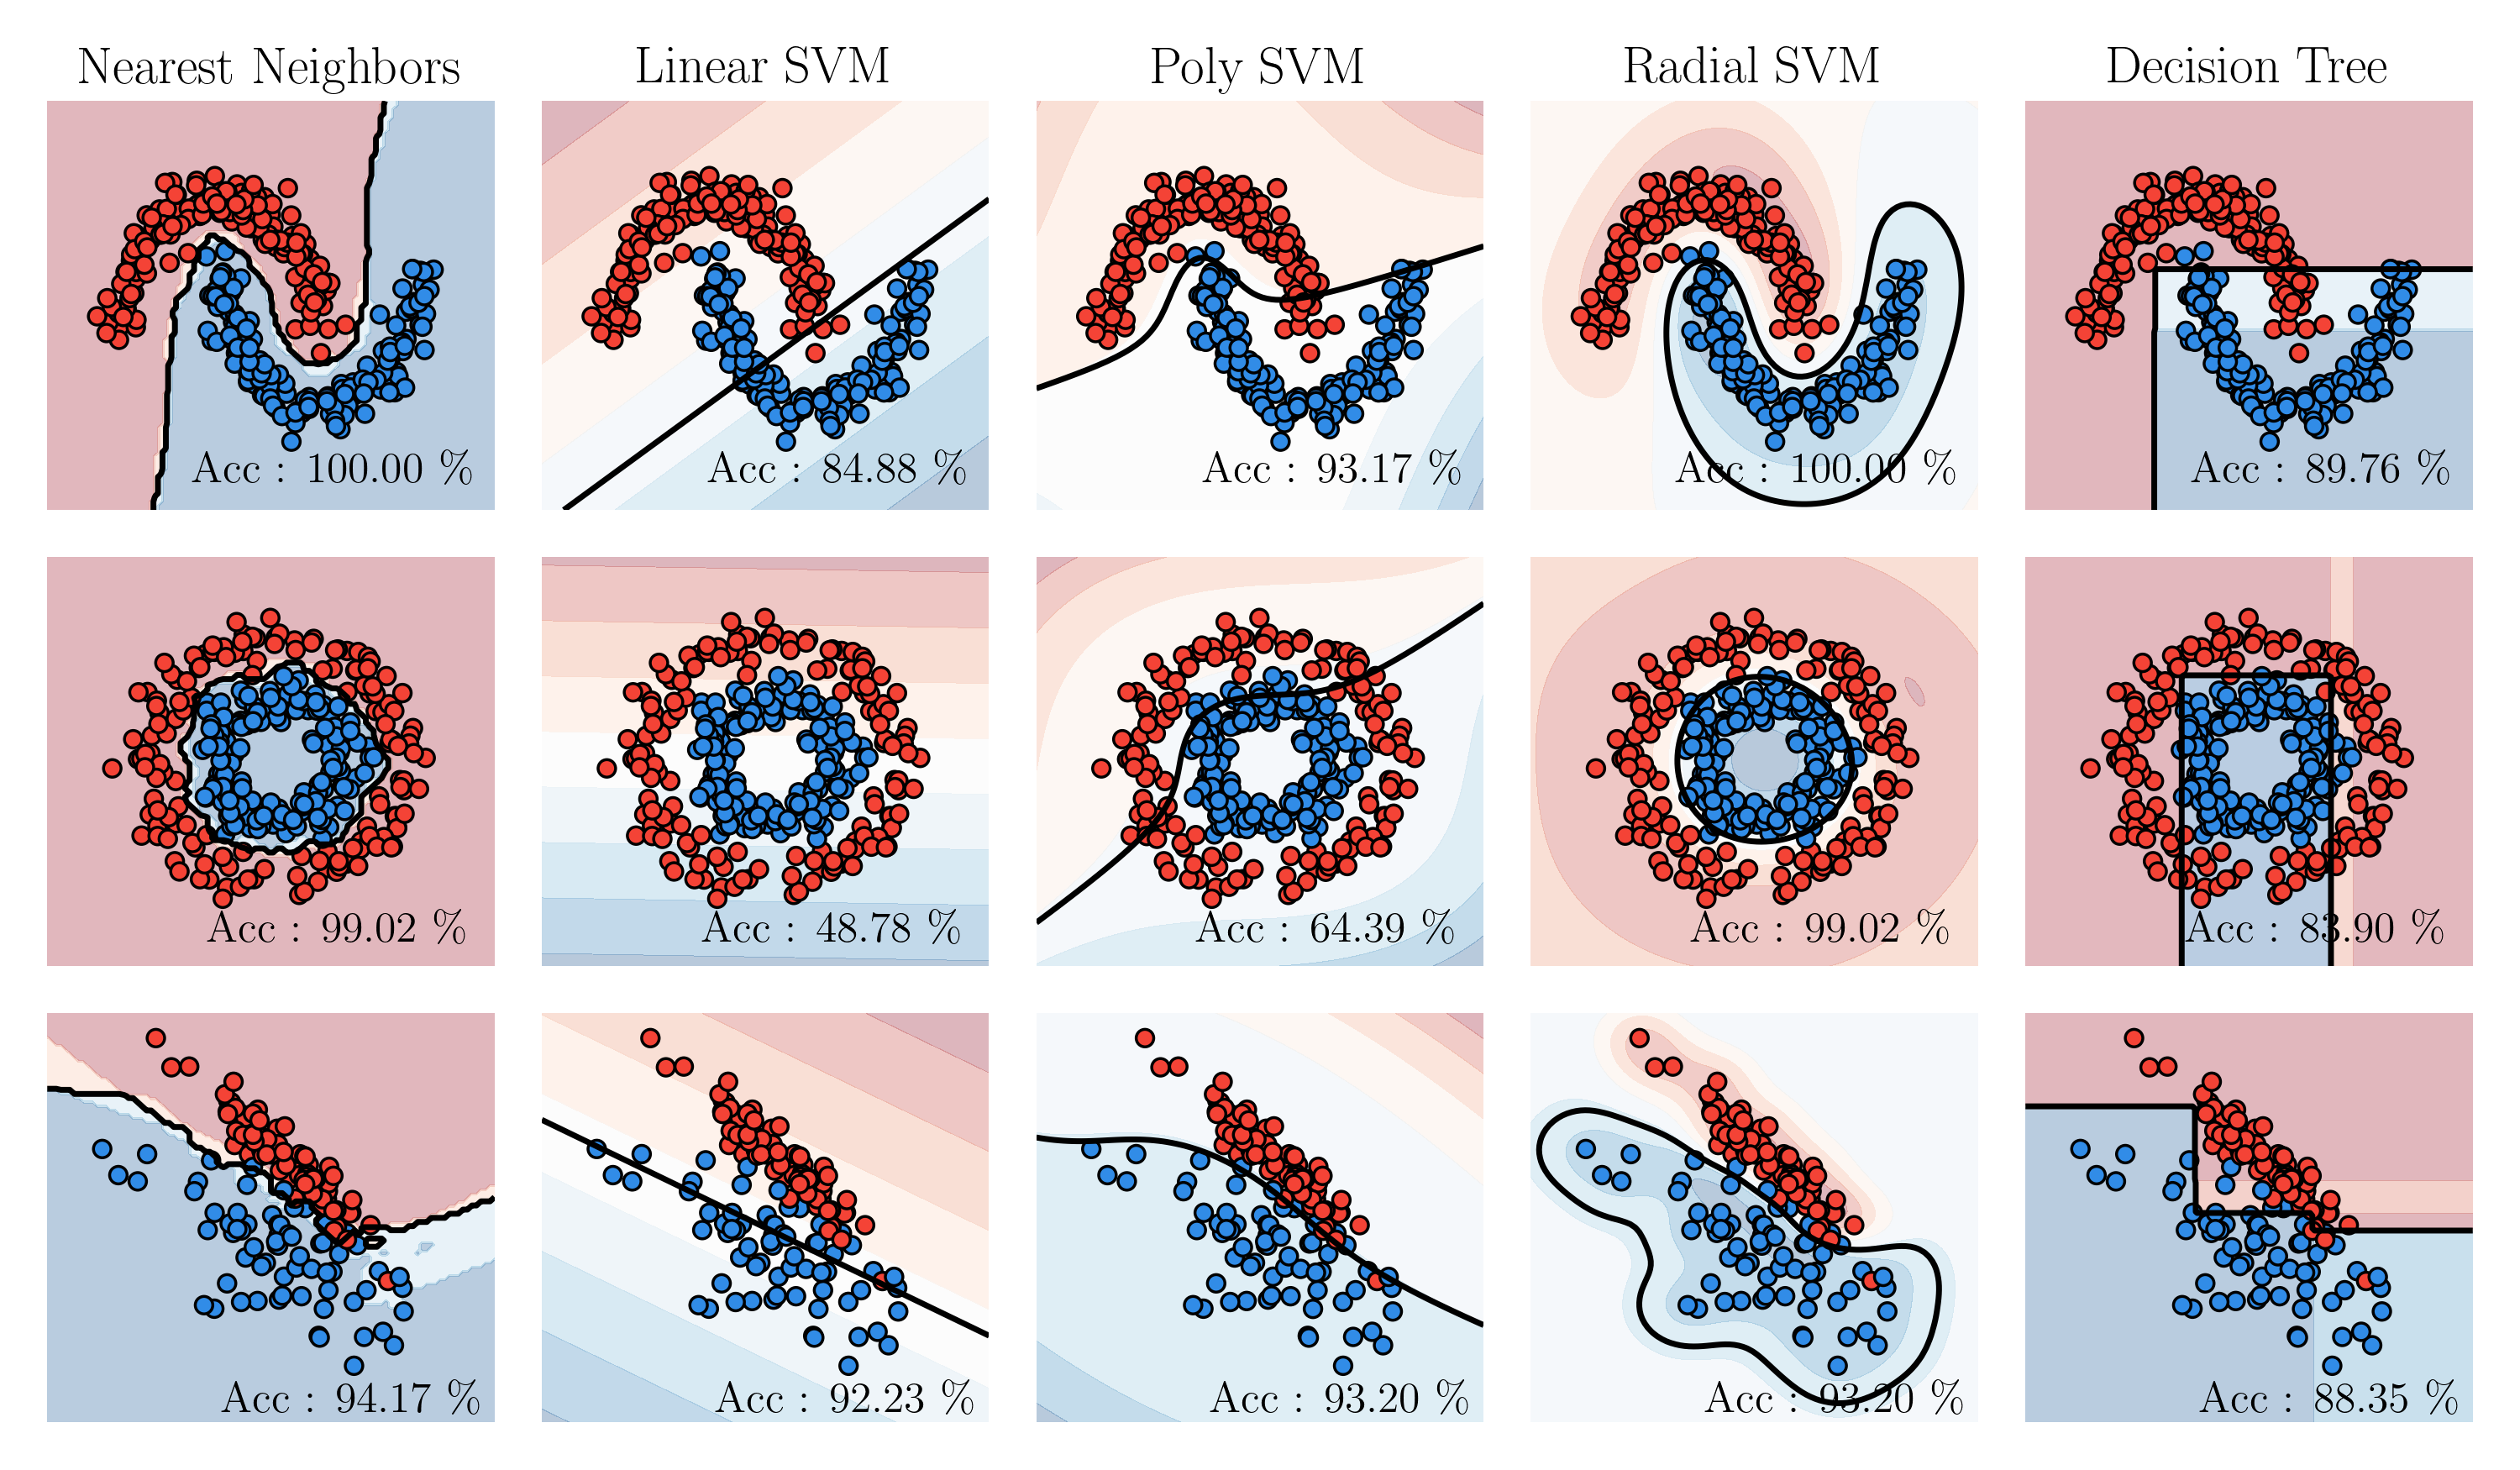
\includegraphics[width=0.8\textwidth]{figures/2Dmodels.png}
		\caption{2D classification for different AI models.}
	\end{figure}
\end{frame}

\begin{frame}{}{The Universal Approximation Theorem}
	The Universal Approximation Theorem is a fundamental result in the field of artificial neural networks. It states that a deep learning model can approximate any function.
	\begin{theorem}[Universal Approximation Theorem]
		Let $\mathcal{ X}\subset \mathbb{R}^d$ be compact, $ \mathcal{Y}\subset \mathbb{R}^m$, $f : \cal X \rightarrow \cal Y$  be a continuous function and $\sigma : \mathbb{R} \rightarrow \mathbb{R}$ be a continuous real function.\newline
		Then $\sigma$ is not polynomial if and only if for every $\epsilon >0$, there exist $k\in \mathbb{N}$, $A\in \mathbb{R}^{k\times d}$, $b\in \mathbb{R}^{k}$ and $C\in \mathbb{R}^{m\times k}$ such that
		$$
			\sup_{x\in \cal X} \Vert f(x)-g(x)\Vert \leq \epsilon
		$$
		where $g(x) = C \times \sigma(Ax+b)$.
	\end{theorem}
\end{frame}

\begin{frame}{}{Classification task}
	\begin{figure}
		\centering
		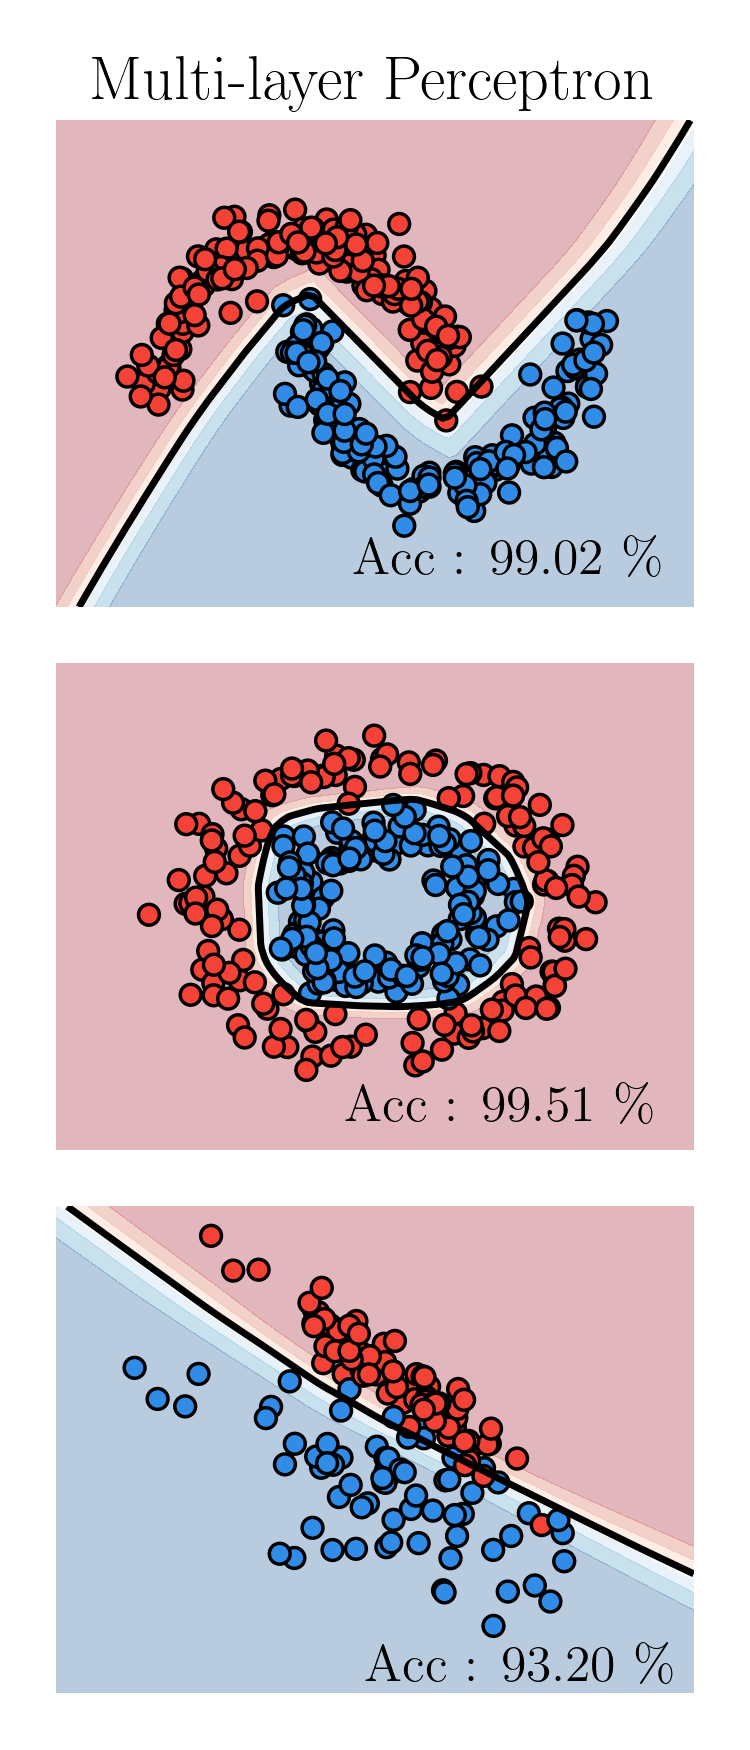
\includegraphics[width=0.2\textwidth]{figures/2DMLP.png}
		\caption{2D classification for small Neural Network.}
	\end{figure}
\end{frame}

\subsection{Representation Learning}


\begin{frame}
	How does deep learning work in practice ?
	\newline

	Deep learning is a subset of representation learning that uses deep neural networks to learn meaningful representations of data. In deep learning, representations are learned through a hierarchy of nonlinear transformations, where each layer of the network builds upon the previous one to extract increasingly abstract and higher-level features from the input data.
	\begin{figure}
		\centering
		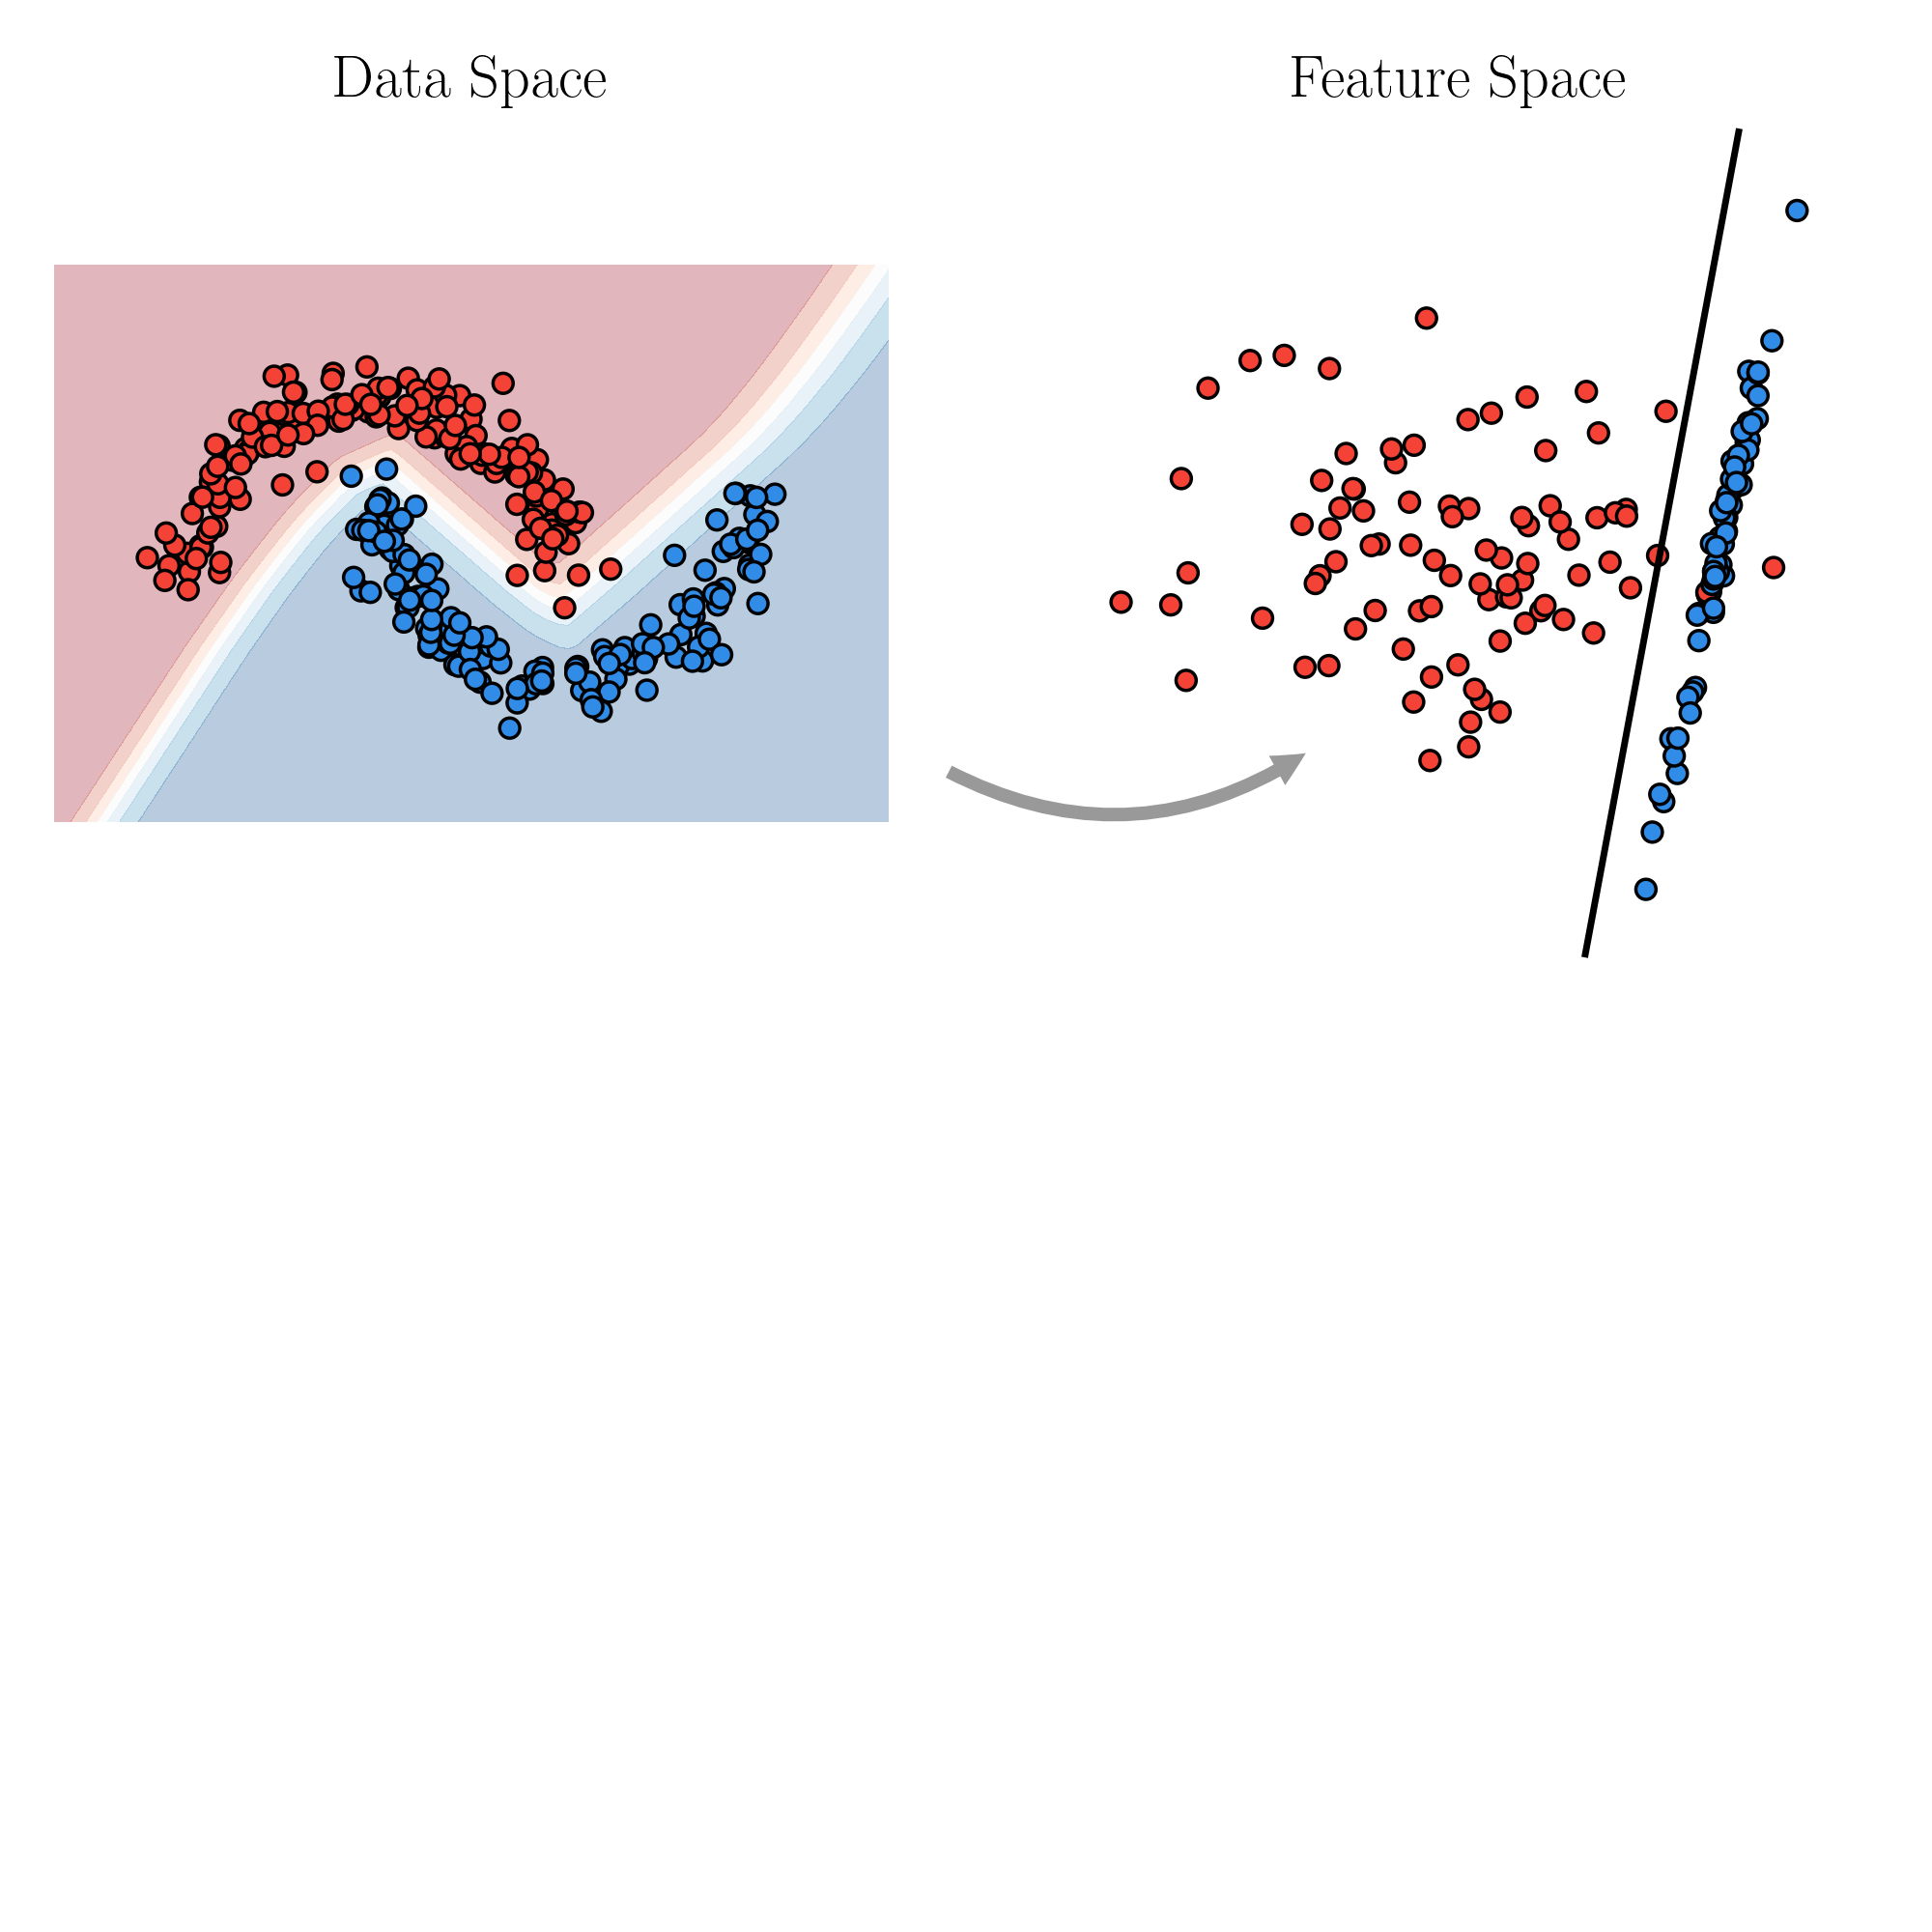
\includegraphics[width=0.6\textwidth]{figures/2DFeature.png}
	\end{figure}
\end{frame}

\begin{frame}{}{Example of Representation Learning}

	\begin{columns}[T,onlytextwidth]
		\column{0.7\textwidth}
		Consider the task of recognizing objects in images. A traditional approach would be to hand-engineer features such as edge detectors and color histograms that can be fed into a classifier. \\
		However, with deep learning representation learning, the model learns to automatically discover these features from the data. The network might start by learning simple features such as edges and color blobs in the first layer, then build upon these to learn more complex features such as parts of objects in subsequent layers, until finally, the final layer outputs a probability distribution over classes of objects. \\

		In this way, deep learning of representation enables the model to automatically learn a rich and meaningful representation of the data, without the need for manual feature engineering.
		\column{0.3\textwidth}
		\begin{figure}
			\centering
			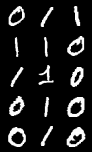
\includegraphics[width=0.7\textwidth]{figures/MNIST.png}
			\caption{MNIST}
		\end{figure}
	\end{columns}
\end{frame}

\begin{frame}{}{Example of Representation Learning}
	\begin{columns}[c,onlytextwidth]
		\column{0.25\textwidth}
		\begin{figure}
			\centering
			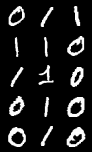
\includegraphics[width=0.7\textwidth]{figures/MNIST.png}
			\caption{MNIST : Layer 0}
		\end{figure}
		\column{0.25\textwidth}
		\begin{figure}
			\centering
			
\includegraphics[width=0.7\textwidth]{figures/MNIST_l1.png}
			\caption{MNIST : Layer 1}
		\end{figure}
		\column{0.5\textwidth}
		\begin{figure}
			\centering
			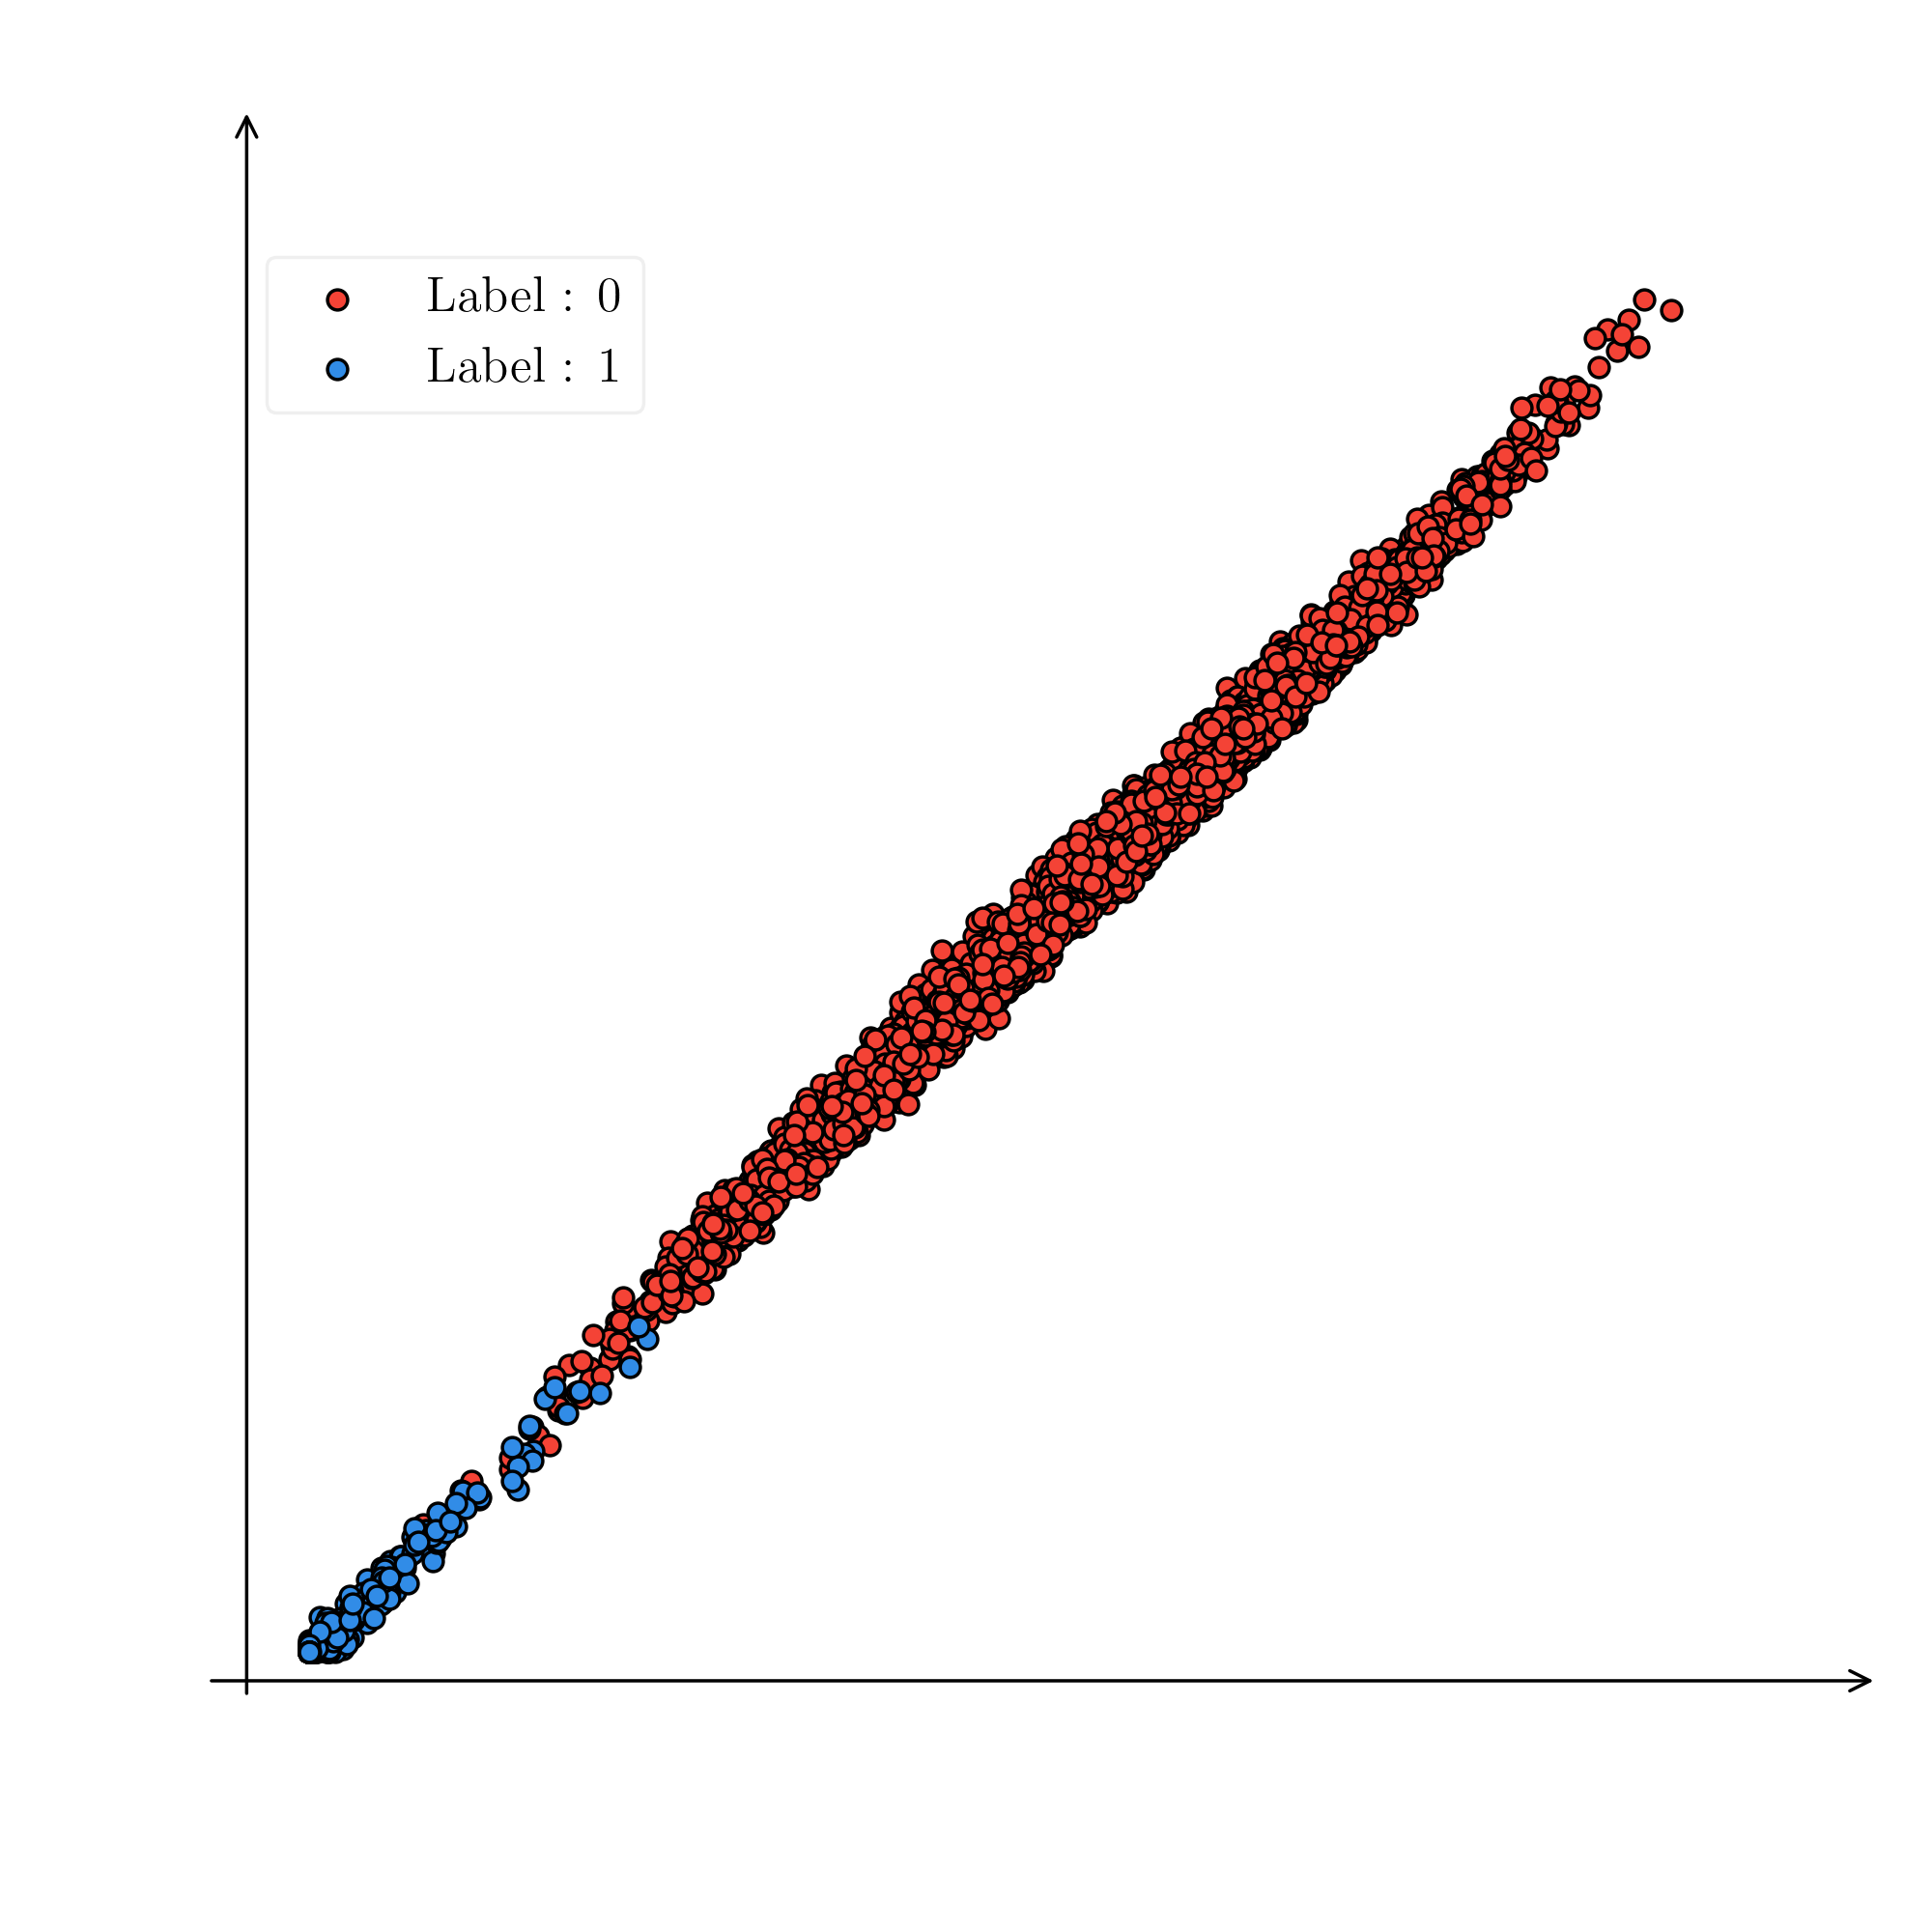
\includegraphics[width=0.9\textwidth]{figures/MNIST_l2.png}
			\caption{MNIST : Layer 2}
		\end{figure}
	\end{columns}
\end{frame}


\begin{frame}{}{Example of Representation Learning}
	\begin{columns}[c,onlytextwidth]
		\column{0.4\textwidth}
		\begin{figure}
			\centering
			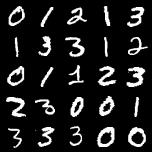
\includegraphics[width=0.7\textwidth]{figures/MNIST_full.png}
			\caption{MNIST : Layer 0}
		\end{figure}
		\column{0.6\textwidth}
		\begin{figure}
			\centering
			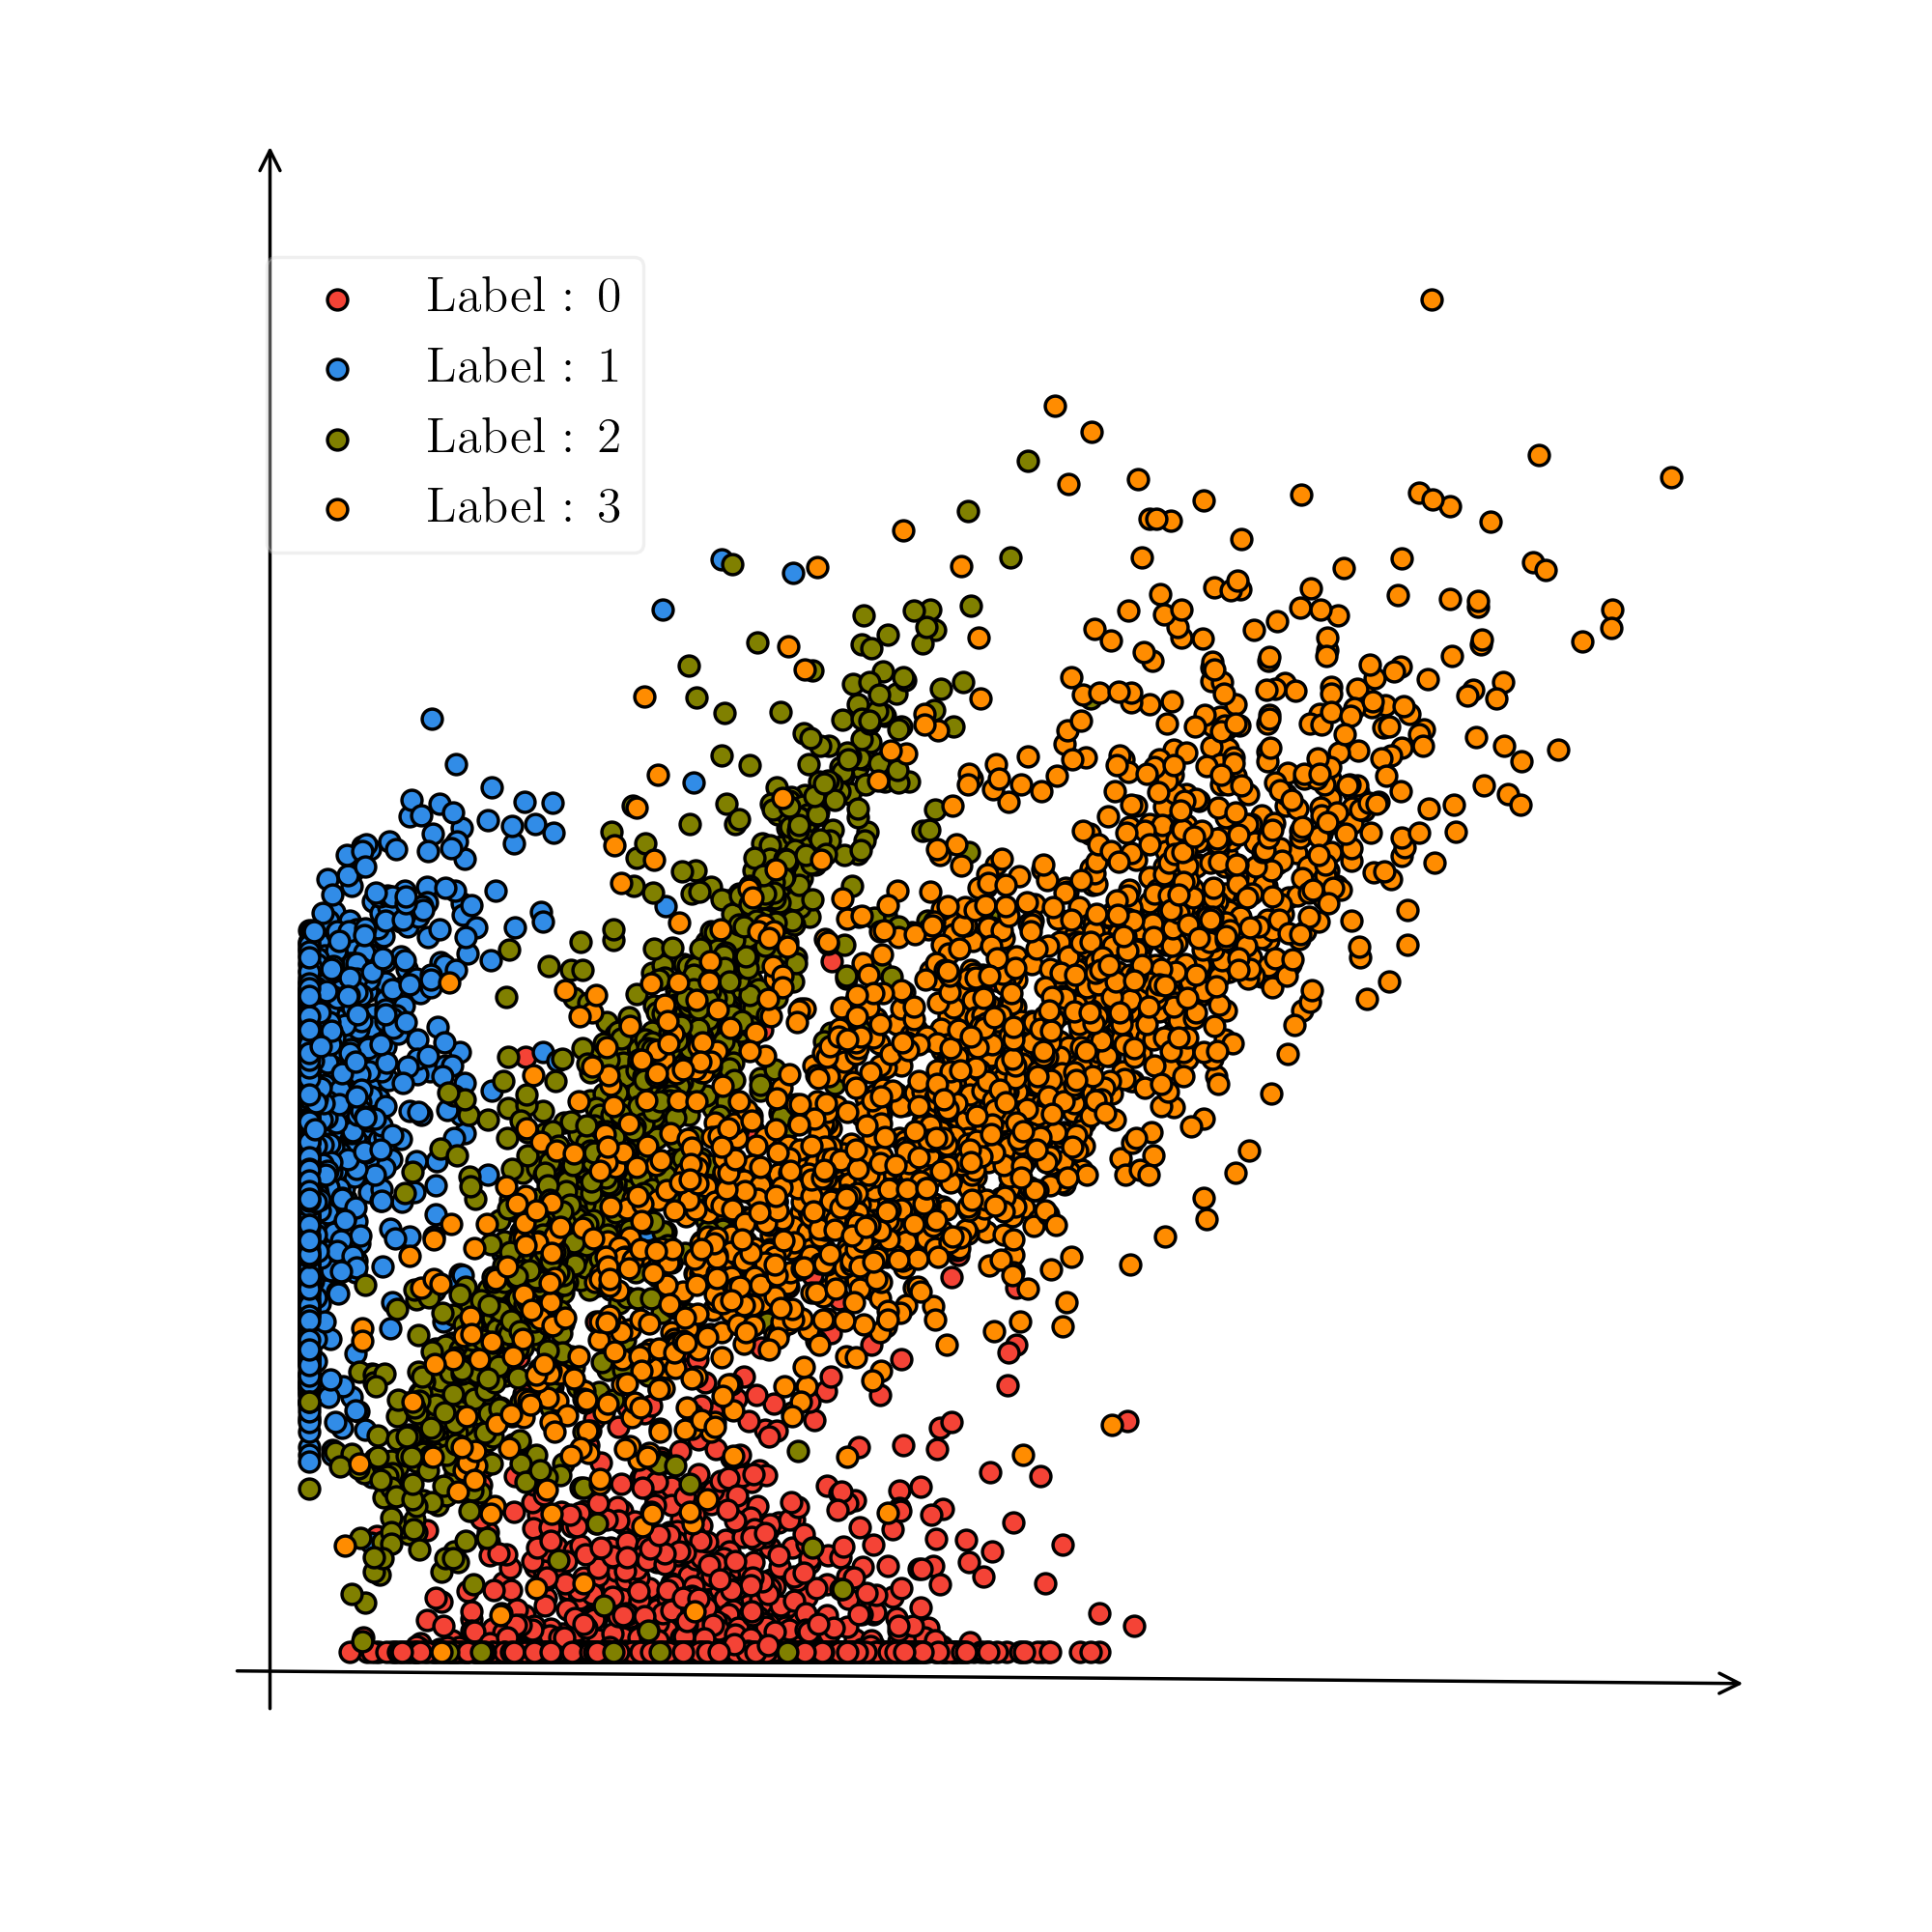
\includegraphics[width=0.7\textwidth]{figures/MNIST_l2_full.png}
			\caption{MNIST : Layer 2}
		\end{figure}
	\end{columns}
\end{frame}


\begin{frame}{}{Deep Learning and Neural Networks}
	Ok, Deep Learning is a model that learns a good representation of the feature. But how?
	\begin{itemize}
		\item How does it work ?
		\item How can we build a model ?
		\item How does it learn ?
	\end{itemize}
\end{frame}

\section{Neural Networks Fundamentals}
\begin{frame}
	Typically, a neural network is defined as a computational model composed of interconnected nodes, organised into layers, that perform transformations on input data.
	\begin{figure}
		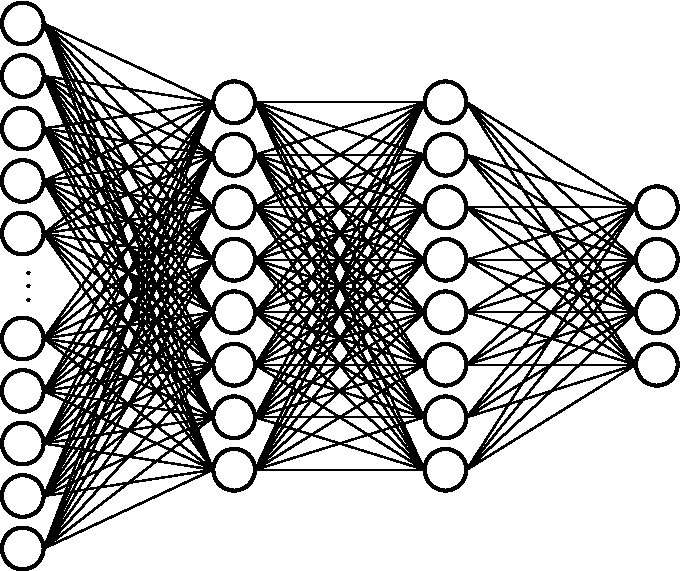
\includegraphics[width = 0.5\textwidth]{figures/ANN.pdf}
	\end{figure}
	Let's see what the interconnected nodes, the layers and the transformations are.

\end{frame}
\subsection{Neurons}
\begin{frame}{}{Neurons}
	If we consider that the Neural Network is a function $f:\mathbb{R}^d\rightarrow \mathbb{R}^m$:
	\begin{figure}
		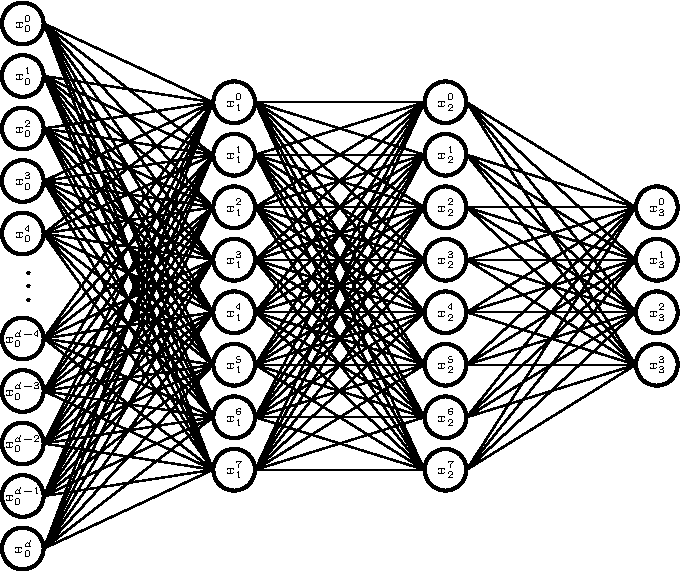
\includegraphics[width = 0.5\textwidth]{figures/ANN_neurons.pdf}
	\end{figure}
	A \alert{Neuron} is a processing unit that receives input, performs a computation, and produces an output. Here, the inputs are $x_{i-1}$ and the output is $x_{i}^k$.
\end{frame}

\begin{frame}
	For example, with an image dataset, the image can be flattened:
	\begin{figure}
		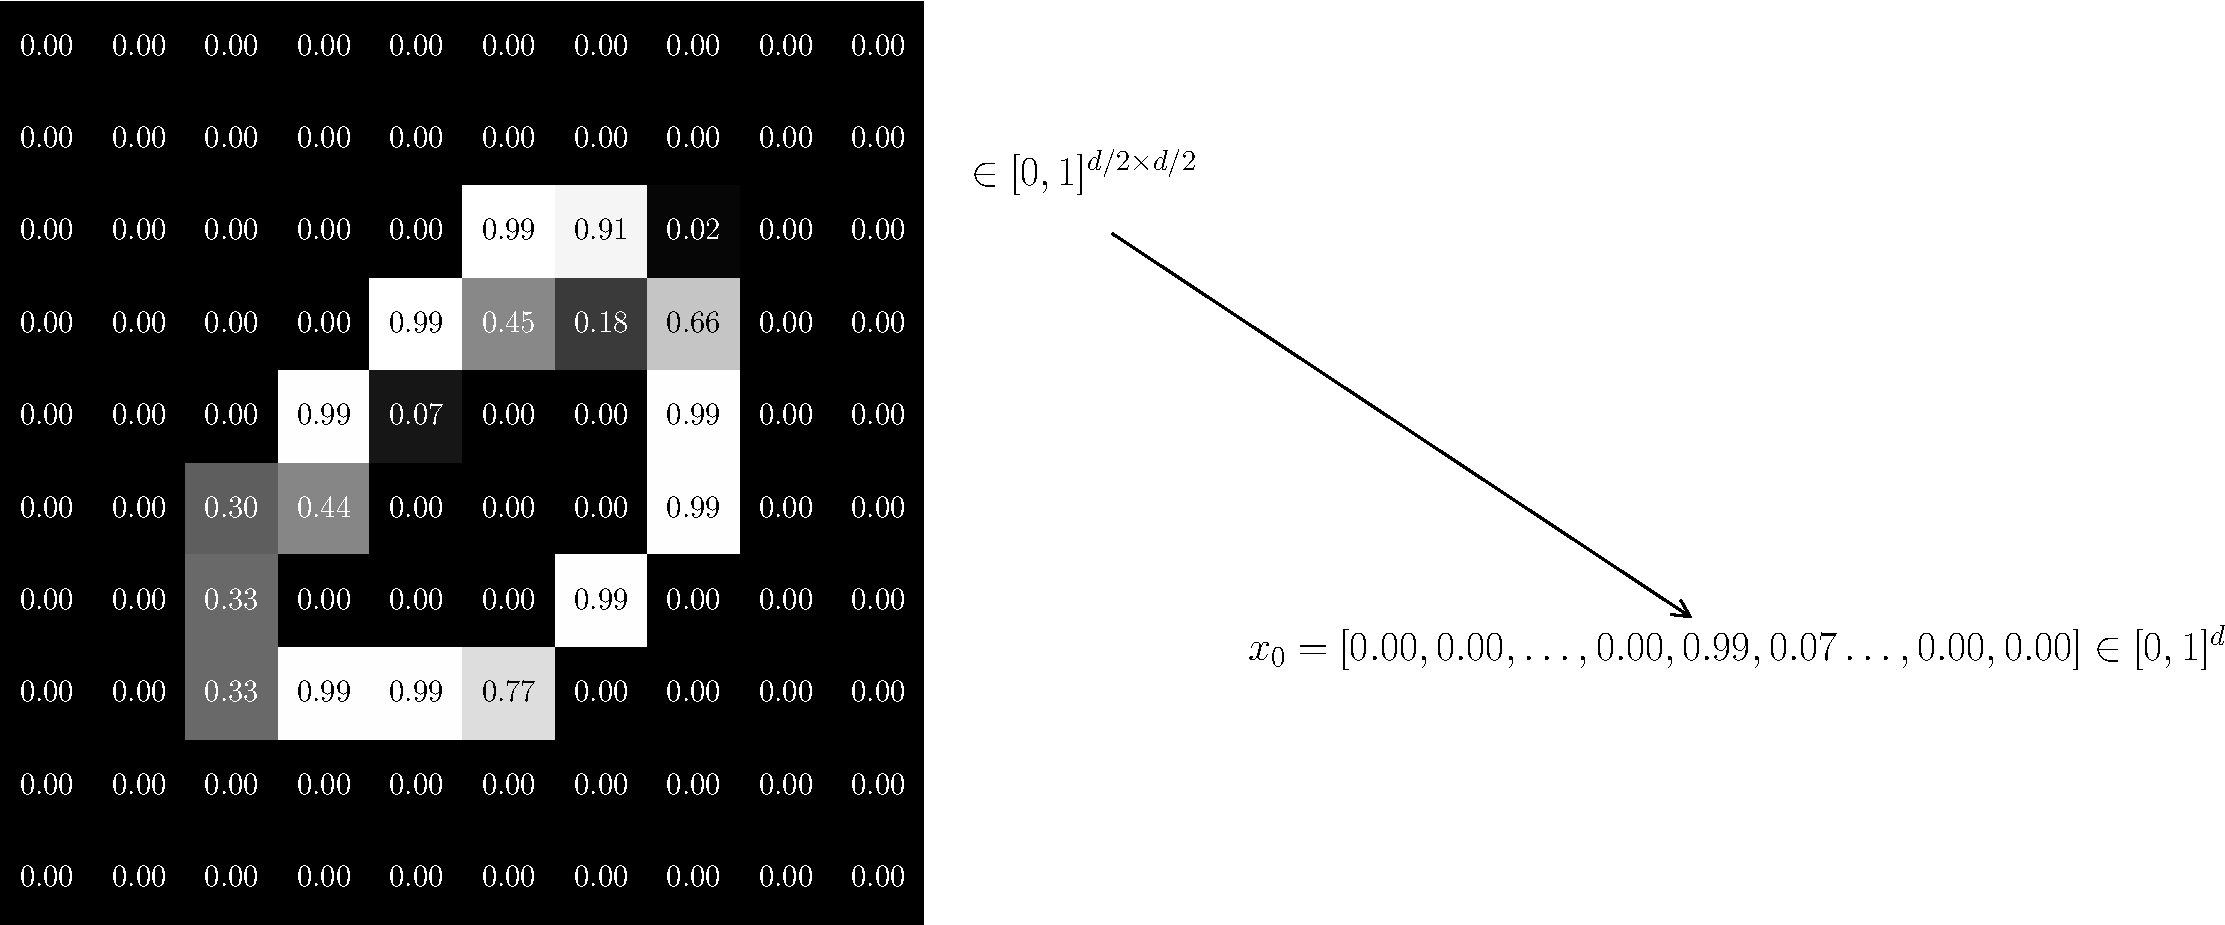
\includegraphics[width = 0.9\textwidth]{figures/mnist2ANN.pdf}
	\end{figure}
\end{frame}

\subsection{Layers}

\begin{frame}
	\begin{columns}[c,onlytextwidth]
		\column{0.3\textwidth}
		A layer $i$ is defined by a matrix $A_i\in\mathbb{R}^{k_{i-1}\times k_{i}}$, a vector $b_i\in\mathbb{R}^{k_{i}}$ and a nonlinear function $\sigma_i:\mathbb{R}\mapsto\mathbb{R}$. The transformation made by a layer is:
		$$x_i =\sigma_i\left(A_ix_{i-1}+b_i\right).$$
		The non-linear function $\sigma_i$ the \alert{activation function}.
		\column{0.7\textwidth}
		\begin{figure}
			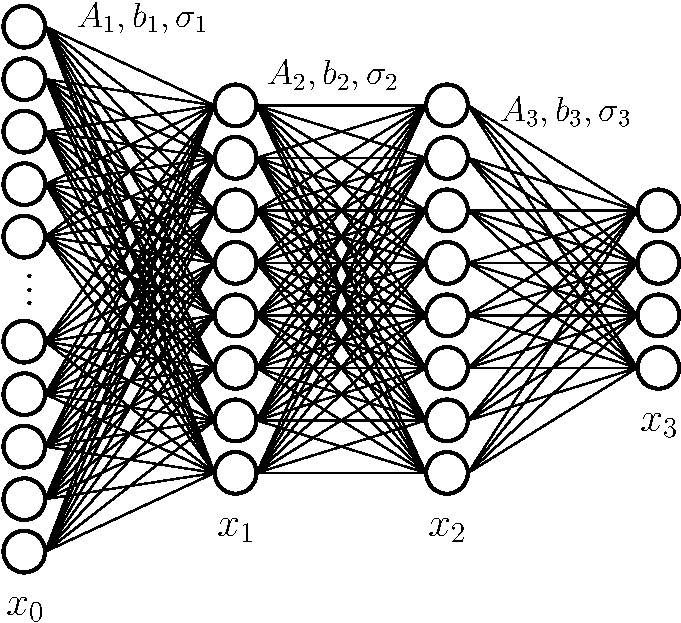
\includegraphics[width = 0.7\textwidth]{figures/ANN_layers.pdf}
		\end{figure}
	\end{columns}
\end{frame}

\begin{frame}
	\begin{columns}[c,onlytextwidth]
		\column{0.3\textwidth}
		A layer $i$ is defined as a matrix $A_i\in\mathbb{R}^{k_{i-1}\times k_{i}}$, a vector $b_i\in\mathbb{R}^{k_{i}}$ and a nonlinear function $\sigma_i:\mathbb{R}\mapsto\mathbb{R}$. The transformation made by a layer is:
		$$x_i^k =\sigma_i\left(\sum_{l=1}^{k_i} \left[A_i\right]_{l,k} x_{i-1}+\left[b_i\right]_k\right).$$
		The non-linear function $\sigma_i$ the \alert{activation function}.
		\column{0.7\textwidth}
		\begin{figure}
			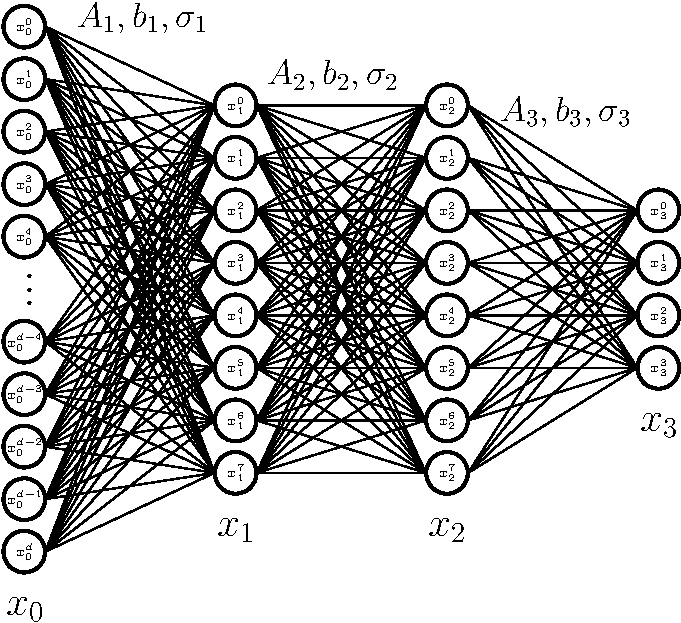
\includegraphics[width = 0.7\textwidth]{figures/ANN_complete.pdf}
		\end{figure}
	\end{columns}
\end{frame}



\subsection{Activation Functions}

\begin{frame}
	The activation functions play a crucial role in the implementation of deep neural networks, as they allow them to approximate any continuous function, as stated by the Universal Approximation Theorem.
	We can list some activation function that are commonly used :
	\begin{itemize}
		\item Linear
		\item Sigmoid
		\item Hyperbolic Tangent
		\item Rectified Linear Unit (ReLU)
		\item Leaky Rectified Linear Unit (Leaky ReLU)
		\item Exponential Linear Unit (ELU)
		\item Sigmoid-Weighted Linear Unit (Swish)
		\item Softmax
	\end{itemize}
\end{frame}

\begin{frame}{}{Linear}
	\begin{columns}[c,onlytextwidth]
		\column{0.3\textwidth}
		\begin{itemize}
			\item Linear activation Function:
			      $$
				      \sigma(x) = x
			      $$
			\item Final activation
			\item Use case : Regression
		\end{itemize}
		\column{0.7\textwidth}

		\begin{figure}
			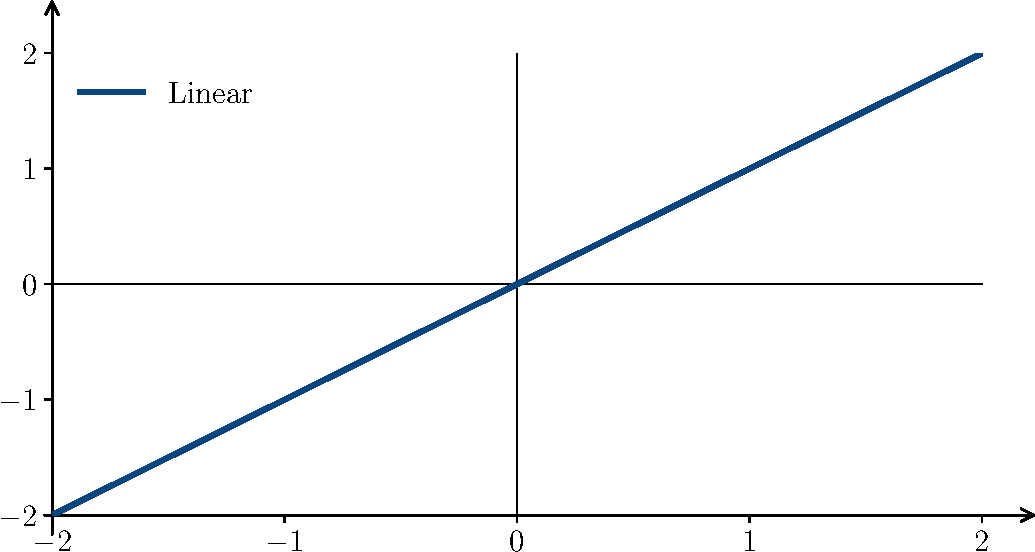
\includegraphics[width = 0.8\textwidth]{figures/linear.pdf}
		\end{figure}
	\end{columns}
\end{frame}

\begin{frame}{}{Sigmoid}
	\begin{columns}[c,onlytextwidth]
		\column{0.3\textwidth}
		\begin{itemize}
			\item Sigmoid Function:
			      $$
				      \sigma(x) = \frac{1}{1+e^{-x}}
			      $$
			\item Final activation
			\item Use case : Classification
		\end{itemize}
		\column{0.7\textwidth}
		\begin{figure}
			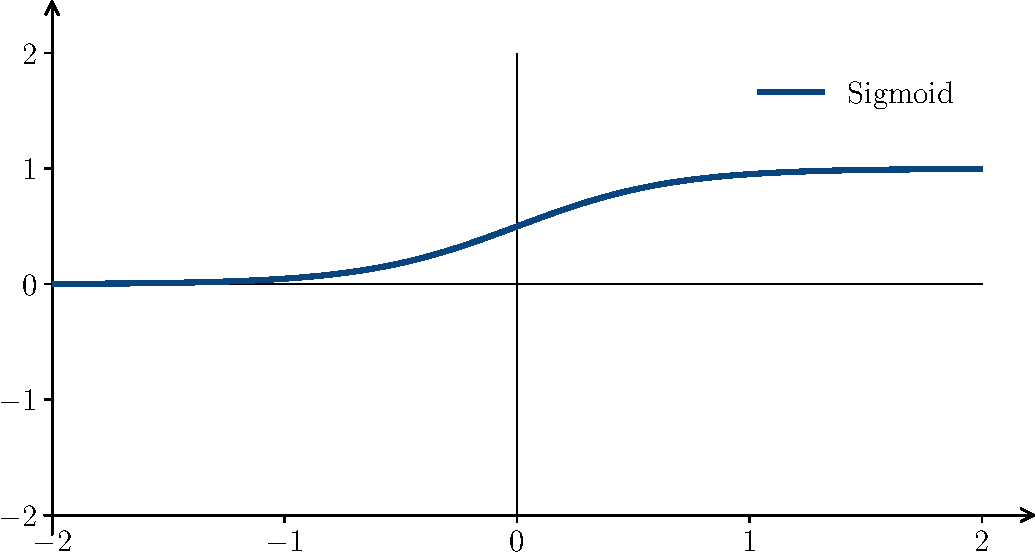
\includegraphics[width = 0.8\textwidth]{figures/sigmoid.pdf}
		\end{figure}
	\end{columns}
\end{frame}

\begin{frame}{}{Softmax}
	\begin{columns}[c,onlytextwidth]
		\column{0.3\textwidth}
		\begin{itemize}
			\item Softmax Function:
			      $$
				      \sigma(x_k) = \frac{e^{x_k}}{\sum_{i=1}^{k_i}e^{x_i}}
			      $$
			\item Final activation
			\item Use case : Multi-class Classification
		\end{itemize}
		\column{0.7\textwidth}
		\begin{figure}
			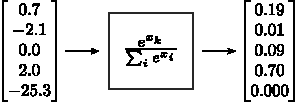
\includegraphics[width = 0.8\textwidth]{figures/softmax.pdf}
		\end{figure}
	\end{columns}
\end{frame}

\begin{frame}{}{Hyperbolic Tangent}
	\begin{columns}[c,onlytextwidth]
		\column{0.3\textwidth}
		\begin{itemize}
			\item Hyperbolic Tangent
			      $$
				      \sigma(x) = \frac{e^x-e^{-x}}{e^x+e^{-x}}
			      $$
			\item Final activation
			\item Use case : Generative task
		\end{itemize}
		\column{0.7\textwidth}
		\begin{figure}
			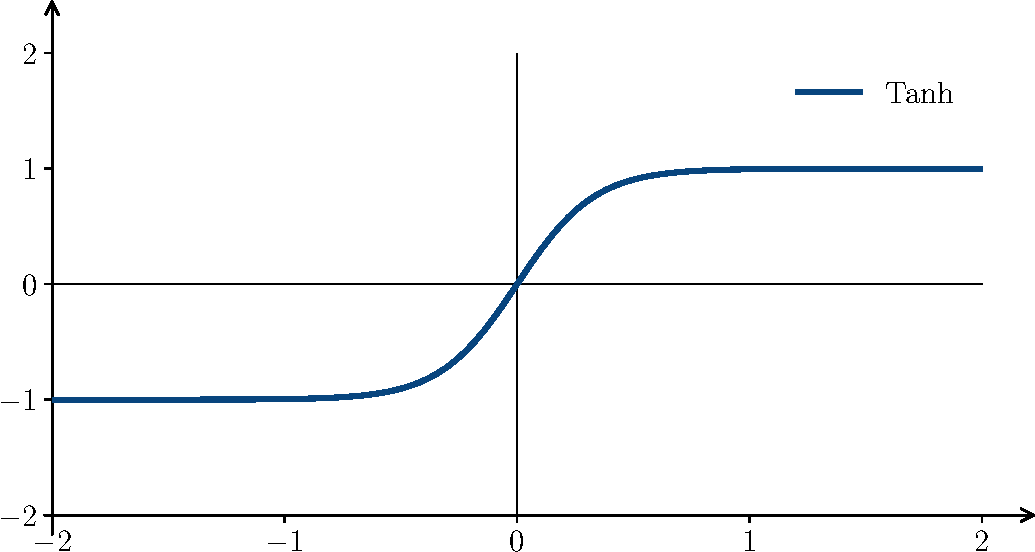
\includegraphics[width = 0.8\textwidth]{figures/tanh.pdf}
		\end{figure}
	\end{columns}
\end{frame}


\begin{frame}{}{ReLU}
	\begin{columns}[c,onlytextwidth]
		\column{0.3\textwidth}
		\begin{itemize}
			\item  Rectified Linear Unit (ReLU):
			      $$
				      \sigma(x) = \max \{0, x\}
			      $$
			\item Intermediate activation
		\end{itemize}
		\column{0.7\textwidth}
		\begin{figure}
			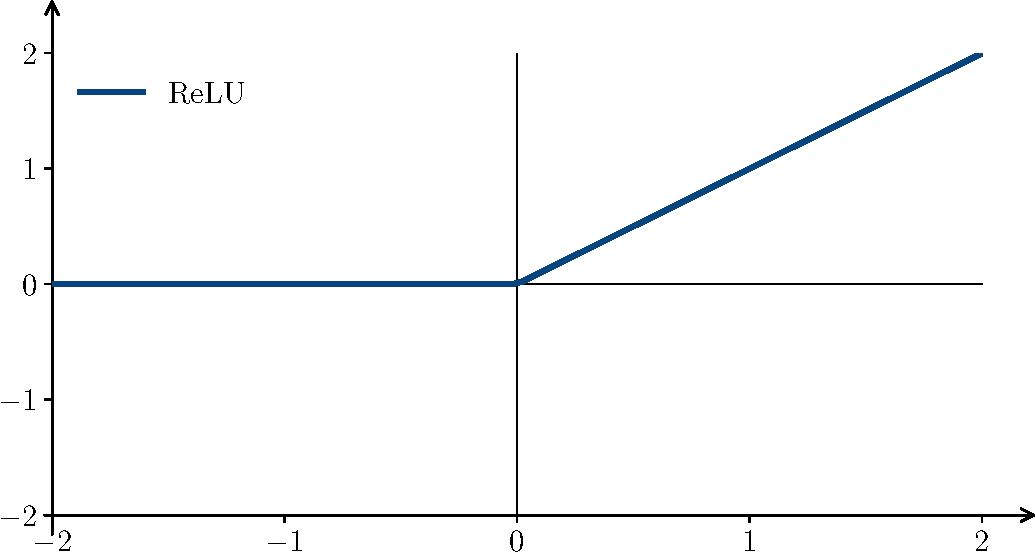
\includegraphics[width = 0.8\textwidth]{figures/relu.pdf}
		\end{figure}
	\end{columns}
\end{frame}

\begin{frame}{}{Leaky ReLU}
	\begin{columns}[c,onlytextwidth]
		\column{0.3\textwidth}
		\begin{itemize}
			\item Leaky  Rectified Linear Unit (Leaky ReLU):
			      $$
				      \sigma(x) = \max \{\alpha x, x\}
			      $$
			\item Intermediate activation
		\end{itemize}
		\column{0.7\textwidth}
		\begin{figure}
			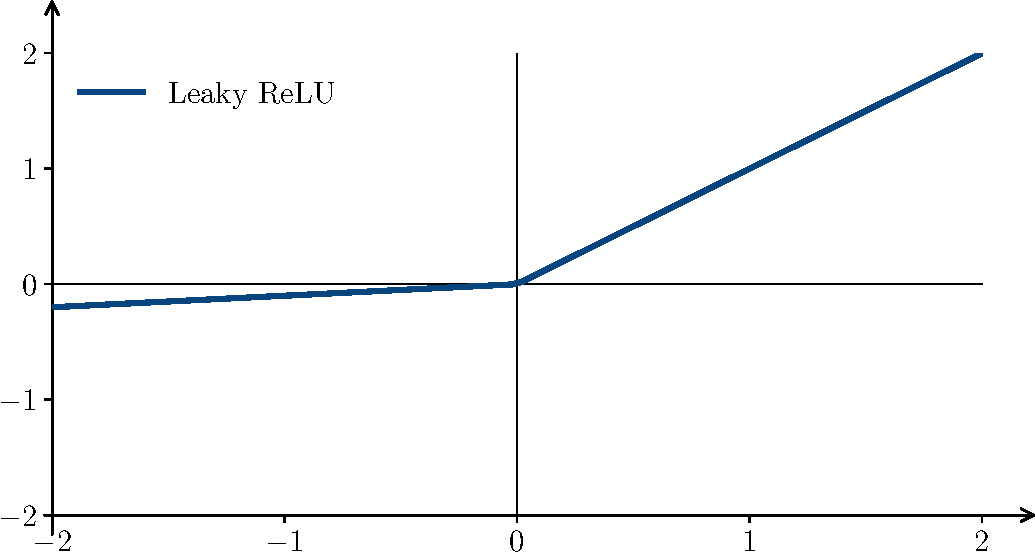
\includegraphics[width = 0.8\textwidth]{figures/leakyrelu.pdf}
		\end{figure}
	\end{columns}
\end{frame}

\begin{frame}{}{ELU}
	\begin{columns}[c,onlytextwidth]
		\column{0.3\textwidth}
		\begin{itemize}
			\item Exponential Linear Unit (ELU):
			      $$
				      \sigma(x) = \begin{cases}
					      \alpha(e^x-1) \quad \mbox{if }x<0, \\
					      x \quad \mbox{if }x\geq0.
				      \end{cases}
			      $$
			\item Intermediate activation
		\end{itemize}
		\column{0.7\textwidth}
		\begin{figure}
			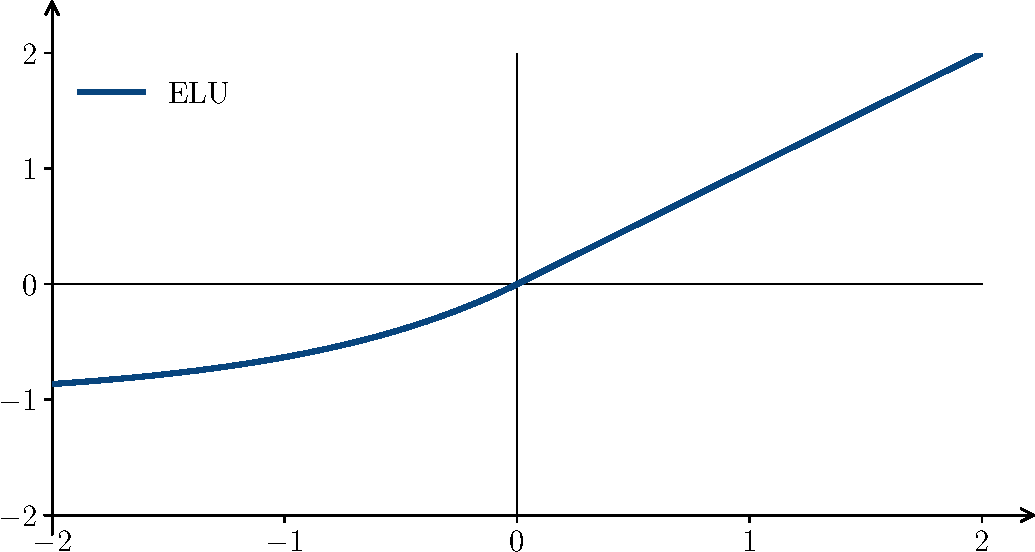
\includegraphics[width = 0.8\textwidth]{figures/elu.pdf}
		\end{figure}
	\end{columns}
\end{frame}

\begin{frame}{}{Swish}
	\begin{columns}[c,onlytextwidth]
		\column{0.3\textwidth}
		\begin{itemize}
			\item Sigmoid-Weighted Linear Unit (Swish):
			      $$
				      \sigma(x) = \frac{x}{1+e^{-x}}
			      $$
			\item Intermediate activation
		\end{itemize}
		\column{0.7\textwidth}
		\begin{figure}
			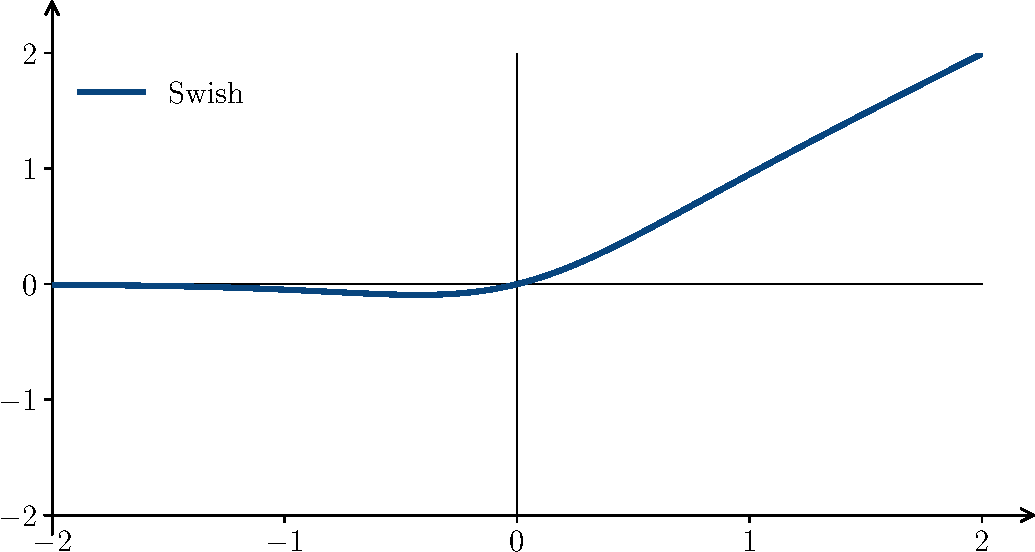
\includegraphics[width = 0.8\textwidth]{figures/swish.pdf}
		\end{figure}
	\end{columns}
\end{frame}


\section{The Multi-layer Perceptron (MLP)}

\begin{frame}
	Having discussed the structure of a neural network, we will proceed to examine the process of training a model for a specific task. As an illustration, we will consider the example of a Multilayer Perceptron.The two intermediate activation functions are ReLUs and the final activation is a softmax to perform multi-class classification on MNIST. We will consider only 4 classes.
	\begin{figure}
		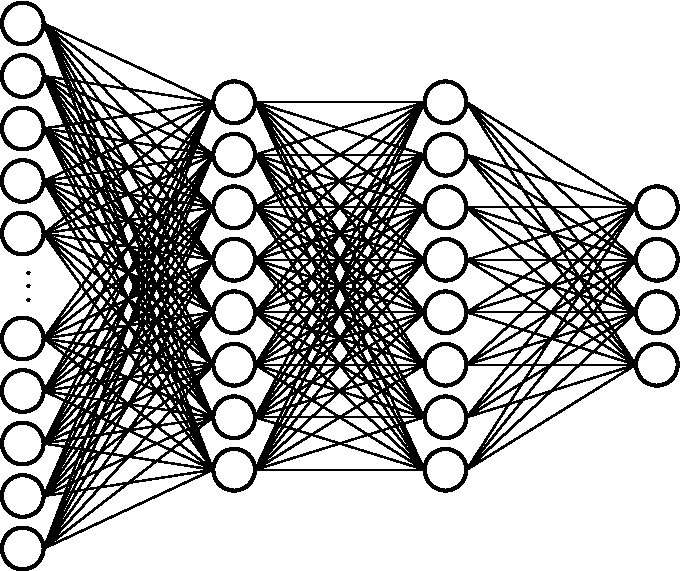
\includegraphics[width = 0.45\textwidth]{figures/ANN.pdf}
	\end{figure}
\end{frame}

\subsection{The first Deep Learning Model}
\begin{frame}
	To introduce the training process, we will consider a 3 layers MLP trained to minimise a loss $\cal L$ over a given a dataset $\cal D$. The model $f_{\theta}$ is parameterised by a vector $\theta=\left\{A_1, A_2, A_3, b_1, b_2, b_3\right\}$:
	$$
		\theta^* = \arg\min_\theta \mathcal{L}( \theta, \mathcal{D})
	$$
	\begin{figure}
		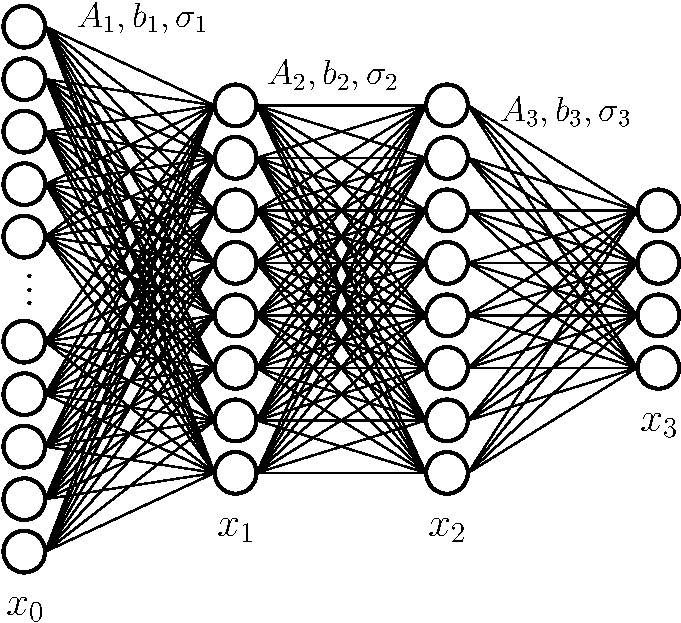
\includegraphics[width = 0.4\textwidth]{figures/ANN_layers.pdf}
	\end{figure}

\end{frame}

\subsection{Stochastic Gradient Descent}

\begin{frame}
	Stochastic gradient descent (SGD) is widely used in deep learning instead of traditional gradient descent due to its efficiency and faster convergence rate. SGD updates the model parameters after computing the gradient of the loss function with respect to each parameter using only a single randomly selected sample. This leads to a faster convergence rate and improved optimization compared to traditional gradient descent, which uses the entire training dataset to compute the gradient at each iteration.

	$$
		\theta^* = \arg \min_\theta \mathcal{L}( \theta, \mathcal{D}) =  \arg \min_\theta \mathbb{E}_{x\sim\mathcal{D}} \left[l(x, f_{\theta}(x))\right]
	$$

\end{frame}
\begin{frame}
	Theoretically the algorithm is the following: \vspace{2cm}
	\begin{algorithm}[H]
		\begin{algorithmic}[1]
			\REQUIRE Given a loss function $l$, a dataset $\mathcal{D}=\{x_1,x_2, \dots, x_N\}$ and a learning rate $\lambda$
			\STATE Initialize parameters $\theta$
			\WHILE {$\theta$ has not converged}
			\FOR{$i = 1$ to $N$}
			\STATE Randomly select $x_i$ from the dataset
			\STATE Compute gradient of the loss with respect to $\theta$: $\nabla_{\theta} l(x_i, f_{\theta}(x_i))$
			\STATE Update parameters $\theta = \theta - \lambda \nabla_{\theta} l(x_i, f(x_i))$
			\ENDFOR
			\ENDWHILE

			\RETURN $\theta$
		\end{algorithmic}
	\end{algorithm}
\end{frame}

\begin{frame}{}{SGD in mini-batch}
	In practice the algorithm is modified to use mini-batches of data instead of single samples. This is done to improve the stability of the optimization process and reduce the variance of the gradient estimates. The algorithm is as follows:

	\vspace{1cm}
	\begin{algorithm}[H]
		\begin{algorithmic}[1]
			\REQUIRE Given a loss function $l$, a dataset $\mathcal{D}=\{x_1,x_2, \dots, x_N\}$, a learning rate $\lambda$ and a batch size $b$
			\STATE Initialize parameters $\theta$
			\STATE Initialize the number of batches $B = \left\lfloor \frac{N}{b}\right\rfloor$
			\WHILE {$\theta$ has not converged}
			\FOR{$i = 1$ to $B$}
			\STATE Randomly select a mini-batch of $b$ samples from the dataset
			\STATE Compute gradient of the loss with respect to $\theta$: $\frac{1}{B}\sum_{i=1}^{B} \nabla_{\theta} l(x_i, f_{\theta}(x_i))$
			\STATE Update parameters $\theta = \theta - \lambda  \frac{1}{B}\sum_{i=1}^{B} \nabla_{\theta}l(x_i, f(x_i))$
			\ENDFOR
			\ENDWHILE
			\RETURN $\theta$
		\end{algorithmic}
	\end{algorithm}
\end{frame}


\subsection{Back-propagation}
\begin{frame}
	At every step $t$ of the gradient descent, setting a learning rate $\lambda$, the parameter $\theta$ is updated as:
	$$
		\theta_{t+1}  = \theta_t - \lambda \nabla_{\theta} l(f(x_i), y_i)
	$$
	But $\theta=\{A_1, A_2, A_3, b_1, b_2, b_3\}$ and the gradient is computed with respect to each parameter.
	\begin{figure}
		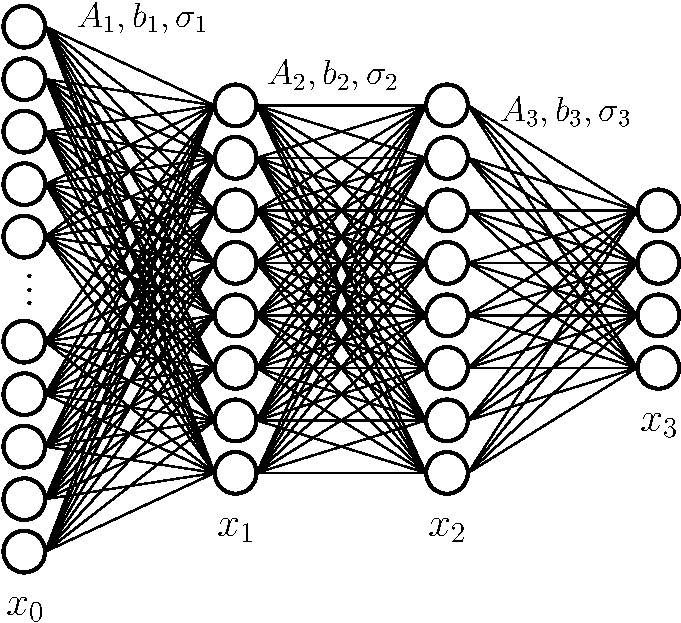
\includegraphics[width = 0.4\textwidth]{figures/ANN_layers.pdf}
	\end{figure}
\end{frame}

\begin{frame}
	First we will consider a single data point $x$, the loss will depend on the output only: $ l(f(x))$.\newline


	$f$ is a layered composed function. Let us focus on the last layer:
	\begin{align*}
		f(x) & = x_3 = \sigma_3(A_3 x_2+b_3)
	\end{align*}
	Therefore:
	\begin{align*}
		l(f(x)) = l\left(\sigma_3\left(A_3x_2+b_3\right)\right)
	\end{align*}
	To minimise the loss, we have to act on $A_3$, $b_3$ and $x_2$.
\end{frame}

\begin{frame}{}{Back-propagation}
	Let us look at the gradients with respect to $A_3$:
	\begin{align*}
		\frac{\partial l}{\partial A_3} & = \frac{\partial l}{\partial x_3}\frac{\partial x_3}{\partial A_3} =l'(x_3)\frac{\partial \sigma_3\left(A_3x_2+b_3\right)}{\partial A_3} = l'(x_3)\sigma_3'\left(A_3x_2+b_3\right)\frac{\partial \left[A_3x_2+b_3\right]}{\partial A_3} \\
		                                & = \underbrace{l'(x_3)}_{\in\mathbb{R}}\:\underbrace{\sigma_3'\left(A_3x_2+b_3\right)}_{\in\mathbb{R}^{k_i\times 1}}\underbrace{x_2^T}_{\in\mathbb{R}^{1\times k_{i-1}}}
	\end{align*}
	and therefore:
	\begin{align*}
		A_3 \leftarrow A_3 - \lambda l'(x_3)\sigma_3'\left(A_3x_2+b_3\right)x_2^T.
	\end{align*}
	We need to keep in memory the latent values of $x$, i.e. $x_2$.
\end{frame}

\begin{frame}{}{Back-propagation}
	Let us look at the gradients with respect to $A_2$:
	\begin{align*}
		\frac{\partial l}{\partial A_2} & = \frac{\partial l}{\partial x_2}\frac{\partial x_2}{\partial A_2}                                                    \\
		                                & =\frac{\partial l}{\partial x_2}\frac{\partial \sigma_2\left(A_2x_1+b_2\right)}{\partial A_2}                         \\
		                                & =\frac{\partial l}{\partial x_2}\sigma_2'\left(A_2x_1+b_2\right)\frac{\partial \left[A_2x_1+b_2\right]}{\partial A_2} \\
		                                & =\frac{\partial l}{\partial x_2} \: \sigma_2'\left(A_2x_1+b_2\right)x_1^T
	\end{align*}
	which depends on $\frac{\partial l}{\partial x_2}$, we need to compute it.
\end{frame}
\begin{frame}{}{Back-propagation}
	We have to compute the gradient with respect to $x_2$:
	\begin{align*}
		\frac{\partial l}{\partial x_2} & = \frac{\partial l}{\partial x_3}\frac{\partial x_3}{\partial x_2} =l'(x_3)\frac{\partial \sigma_3\left(A_3x_2+b_3\right)}{\partial x_2} = l'(x_3)\frac{\partial \left[A_3x_2+b_3\right]}{\partial x_2}\sigma_3'\left(A_3x_2+b_3\right) \\
		                                & =l'(x_3)\:A_3^T\sigma_3'\left(A_3x_2+b_3\right)
	\end{align*}
	Therefore:
	\begin{align*}
		A_2 \leftarrow A_2 - \lambda \left[l'(x_3)A_3^T\sigma_3'\left(A_3x_2+b_3\right) \times  \sigma_2'\left(A_2x_1+b_2\right)x_1^T \right]
	\end{align*}
	The update of $A_2$ depends on $l'(x_3)$,
\end{frame}


\begin{frame}{Back-propagation}
	We have to compute the gradient with respect to $A_1$:
	\begin{align*}
		\frac{\partial l}{\partial A_1} & = \frac{\partial l}{\partial x_1}\frac{\partial x_1}{\partial A_1}                            \\
		                                & =\frac{\partial l}{\partial x_1}\frac{\partial \sigma_1\left(A_1x_0+b_1\right)}{\partial A_1} \\
		                                & =\frac{\partial l}{\partial x_1} \sigma_1'\left(A_1x_0+b_0\right)x_0^T,
	\end{align*}
	which depends on $\frac{\partial l}{\partial x_1}$, we need to compute it.
\end{frame}

\begin{frame}{Back-Propagation}
	Let us compute the gradient with respect to $x_1$:
	\begin{align*}
		\frac{\partial l}{\partial x_1} & = \frac{\partial l}{\partial x_2}\frac{\partial x_2}{\partial x_1} = \frac{\partial l}{\partial x_2}\frac{\partial \sigma_2\left(A_2x_1+b_2\right)}{\partial x_1} =  \frac{\partial l}{\partial x_2}\frac{\partial \left[A_2x_1+b_2\right]}{\partial x_1}\sigma_2'\left(A_2x_1+b_2\right) \\
		                                & = \frac{\partial l}{\partial x_2}A_2^T\sigma_2'\left(A_2x_1+b_2\right)
	\end{align*}
	Therefore:
	\begin{align*}
		A_1 \leftarrow A_1 - \lambda \left[l'(x_3)\:A_3^T\sigma_3'\left(A_3x_2+b_3\right)A_2^T\sigma_2'\left(A_2x_1+b_2\right) \times  \sigma_1'\left(A_1x_0+b_1\right)x_0^T \right]
	\end{align*}
\end{frame}

\begin{frame}{Back-Propagation}
	In other words, the update on the weights is:
	\begin{align*}
		A_3 & \leftarrow A_3 - \lambda l'(x_3)\sigma_3'\left(A_3x_2+b_3\right)x_2^T                                                                                                    \\
		A_2 & \leftarrow A_2 - \lambda \left[l'(x_3)A_3^T\sigma_3'\left(A_3x_2+b_3\right) \times  \sigma_2'\left(A_2x_1+b_2\right)x_1^T \right]                                        \\
		A_1 & \leftarrow A_1 - \lambda \left[l'(x_3)\:A_3^T\sigma_3'\left(A_3x_2+b_3\right)A_2^T\sigma_2'\left(A_2x_1+b_2\right) \times  \sigma_1'\left(A_1x_0+b_1\right)x_0^T \right]
	\end{align*}
\end{frame}



\begin{frame}
	If we look at the update of the different biases, we can easily compute the different gradient and see the updates.
	First, let us compute the gradient with respect to $b_3$:
	\begin{align*}
		\frac{\partial l}{\partial b_3} & = \frac{\partial l}{\partial x_3}\frac{\partial x_3}{\partial b_3}                                                  \\
		                                & =l'(x_3)\frac{\partial \sigma_3\left(A_3x_2+b_3\right)}{\partial b_3}                                               \\
		                                & = l'(x_3)\sigma_3'\left(A_3x_2+b_3\right)\frac{\partial \left[A_3x_2+b_3\right]}{\partial b_3}                      \\
		                                & = \underbrace{l'(x_3)}_{\in\mathbb{R}}\:\underbrace{\sigma_3'\left(A_3x_2+b_3\right)}_{\in\mathbb{R}^{k_i\times 1}}
	\end{align*}
	And thus :
	$$
		b_3 \leftarrow b_3 - \lambda l'(x_3)\sigma'\left(A_3x_2+b_3\right)
	$$
\end{frame}
\begin{frame}
	Let's move on the second layer:
	\begin{align*}
		\frac{\partial l}{\partial b_2} & = \frac{\partial l}{\partial x_2}\frac{\partial x_2}{\partial b_2}                            \\
		                                & =\frac{\partial l}{\partial x_2}\frac{\partial \sigma_2\left(A_2x_1+b_2\right)}{\partial b_2} \\
		                                & =\frac{\partial l}{\partial x_2} \sigma_2'\left(A_2x_1+b_2\right)                             \\
	\end{align*}
	And thus :
	$$
		b_2 \leftarrow b_2 - \lambda	\frac{\partial l}{\partial x_2} \sigma'\left(A_2x_1+b_2\right)
	$$
	We need to back-propagate the term $\frac{\partial l}{\partial x_2}$ computed for the first layer.
\end{frame}

\begin{frame}
	For the first layer:
	\begin{align*}
		\frac{\partial l}{\partial b_1} & = \frac{\partial l}{\partial x_1}\frac{\partial x_1}{\partial b_1}                            \\
		                                & =\frac{\partial l}{\partial x_1}\frac{\partial \sigma_1\left(A_1x_0+b_1\right)}{\partial b_1} \\
		                                & =\frac{\partial l}{\partial x_1} \sigma_1'\left(A_1x_0+b_0\right)                             \\
	\end{align*}
	And thus :
	$$
		b_1 \leftarrow b_1 - \lambda	\frac{\partial l}{\partial x_1} \sigma'\left(A_1x_0+b_1\right)
	$$
	We need to back-propagate the term $\frac{\partial l}{\partial x_1}$ computed for the second layer which has been computed with $\frac{\partial l}{\partial x_2}$ back-propagated from the first layer.
\end{frame}

\begin{frame}{}{Back-Propagation}
	To update the weights, we need to compute the gradient of the loss with respect to the output of the network, and then \textbf{back-propagate} the gradient of the loss with respect to each activation, the $\frac{\partial l}{\partial x_i}$, through the network to compute the gradients with respect to the weights and biases of each layer.
\end{frame}

\begin{frame}{}{Last Layer}
	\begin{columns}[c,onlytextwidth]
		\column{0.3\textwidth}
		We can plot the current state of the network for a given input.\newline

		The red lines show positive values for $A_i$, the blue lines represent negative values for $A_i$.
		The level of transparency is proportional to the previous neurons.
		\column{0.7\textwidth}

		\begin{figure}
			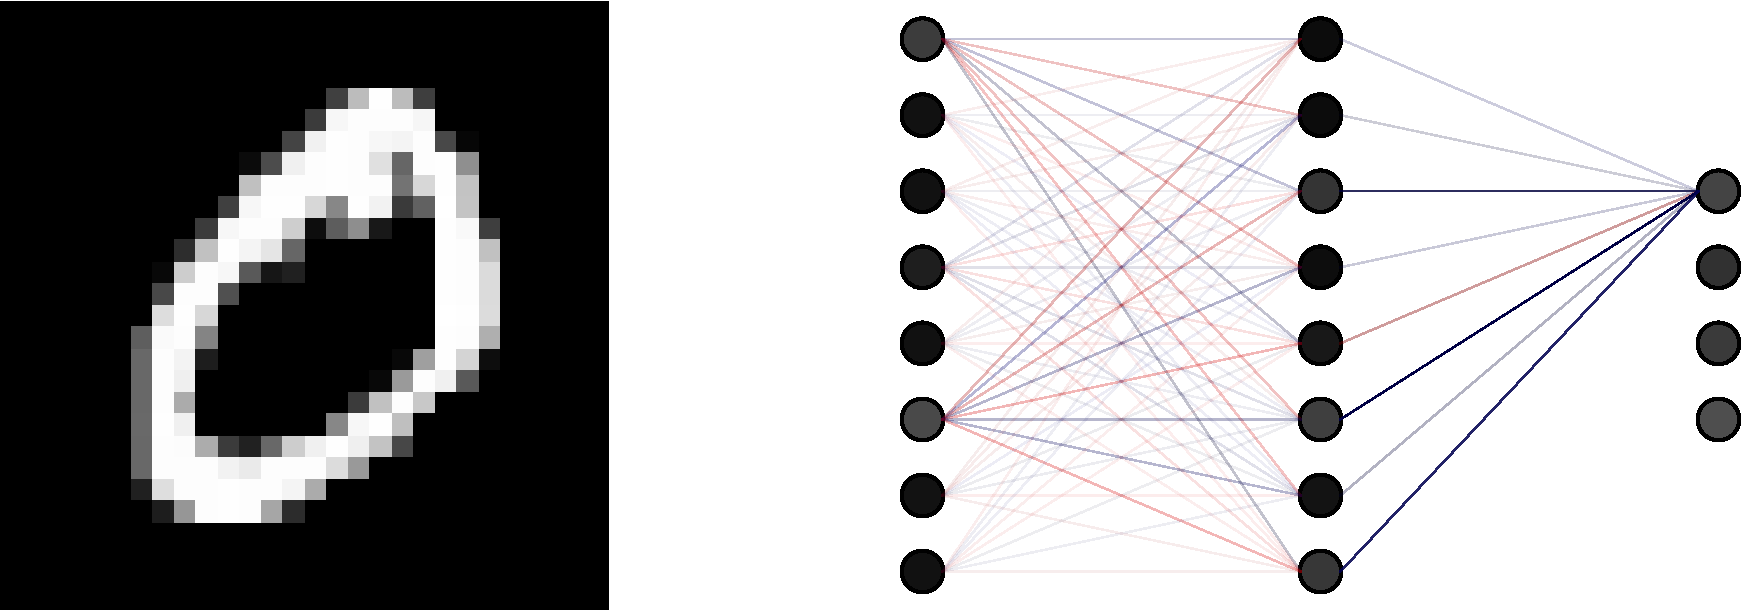
\includegraphics[width=0.9\textwidth]{figures/backpropimg0.pdf}
		\end{figure}
	\end{columns}
	\vfill
	$$
		x_3^1 = \sigma_3\left(A_{3}^{1,1}x_2^1+A_{3}^{1,2}x_2^2 +\dots+A_{3}^{1,8}x_2^8\right)
	$$
\end{frame}

\begin{frame}
	\begin{columns}[c,onlytextwidth]
		\column{0.3\textwidth}
		Iteratively, the neural networks improves its performance.
		\column{0.7\textwidth}

		\begin{figure}
			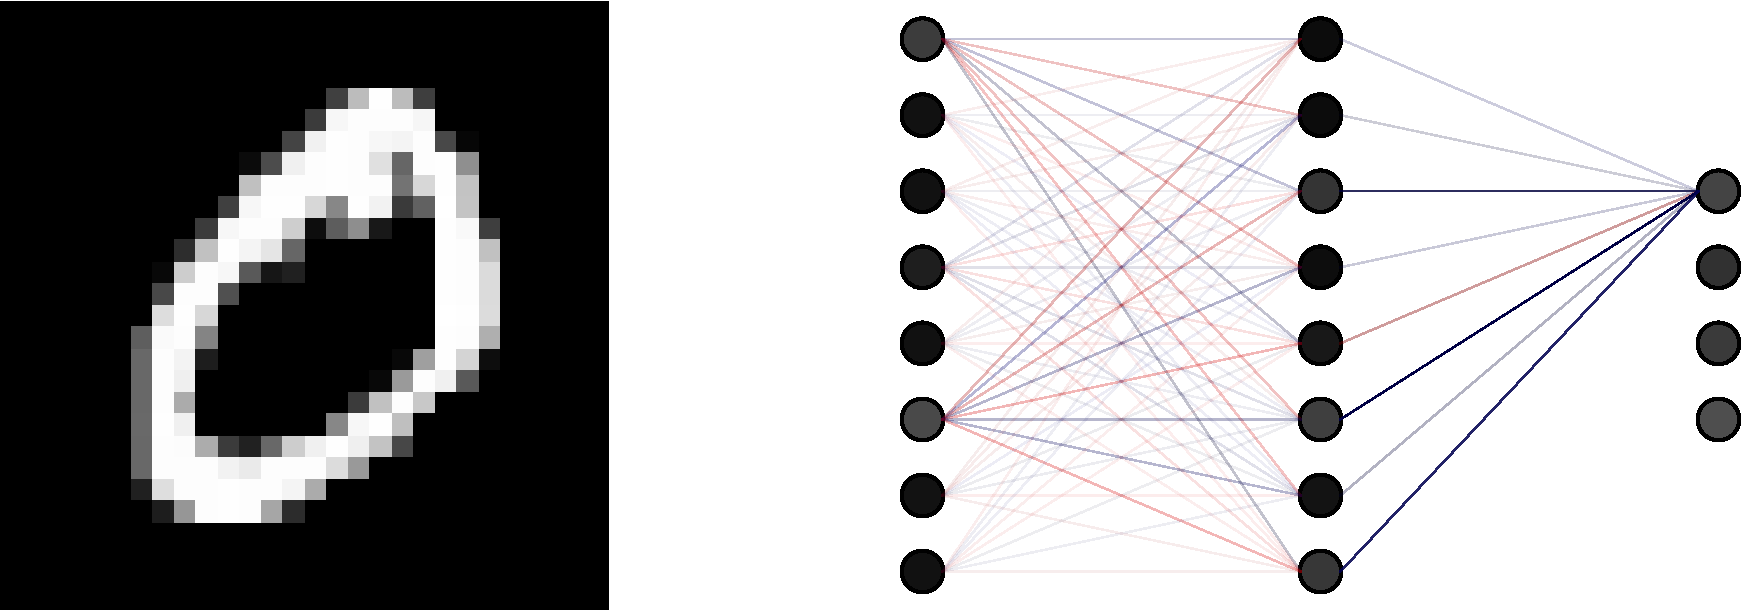
\includegraphics[width=0.9\textwidth]{figures/backpropimg0.pdf}
		\end{figure}
	\end{columns}
	\vfill
	$$
		x_3^1 = \sigma_3\left(A_{3}^{1,1}x_2^1+A_{3}^{1,2}x_2^2 +\dots+A_{3}^{1,8}x_2^8\right)
	$$
\end{frame}

\begin{frame}
	\begin{columns}[c,onlytextwidth]
		\column{0.3\textwidth}
		Iteratively, the neural networks improves its performance.
		\column{0.7\textwidth}

		\begin{figure}
			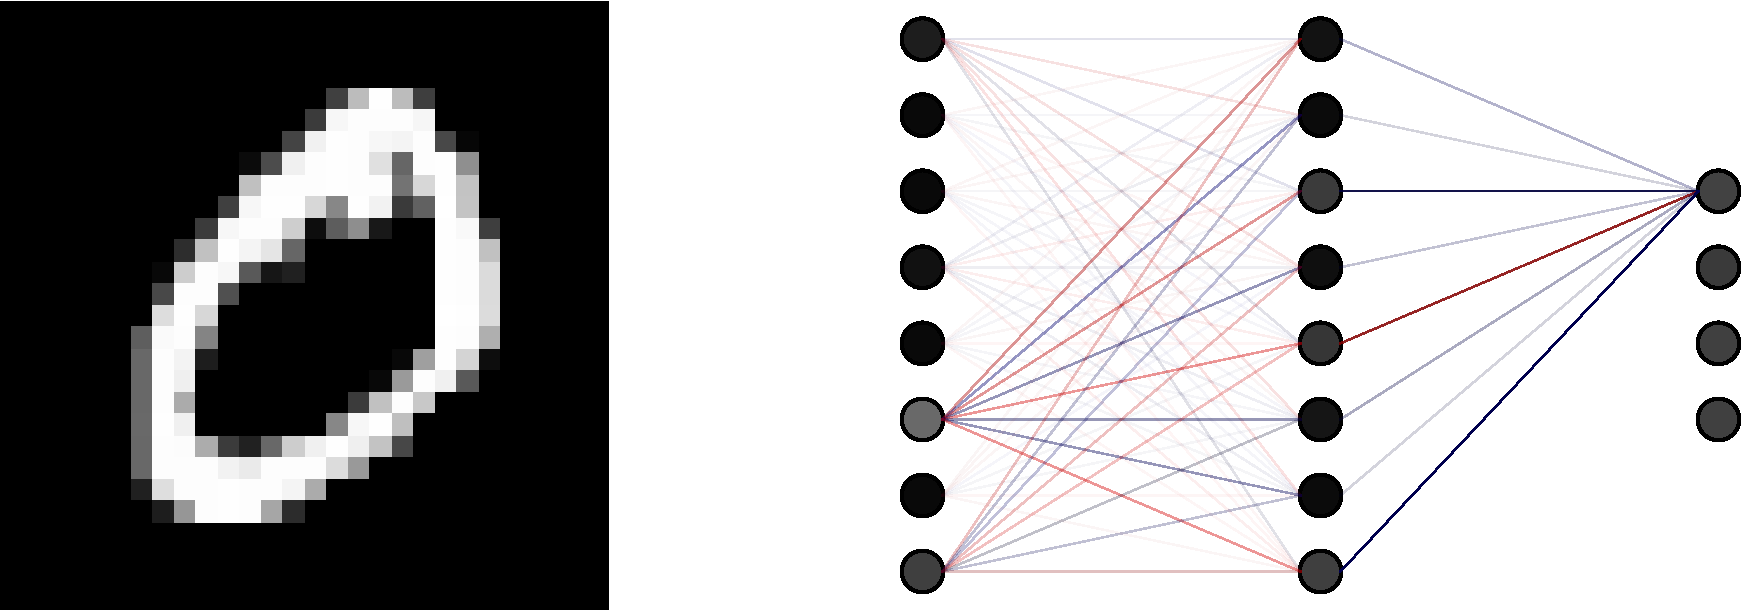
\includegraphics[width=0.9\textwidth]{figures/backpropimg1.pdf}
		\end{figure}
	\end{columns}
	\vfill
	$$
		x_3^1 = \sigma_3\left(A_{3}^{1,1}x_2^1+A_{3}^{1,2}x_2^2 +\dots+A_{3}^{1,8}x_2^8\right)
	$$
\end{frame}
\begin{frame}
	\begin{columns}[c,onlytextwidth]
		\column{0.3\textwidth}
		Iteratively, the neural networks improves its performance.
		\column{0.7\textwidth}

		\begin{figure}
			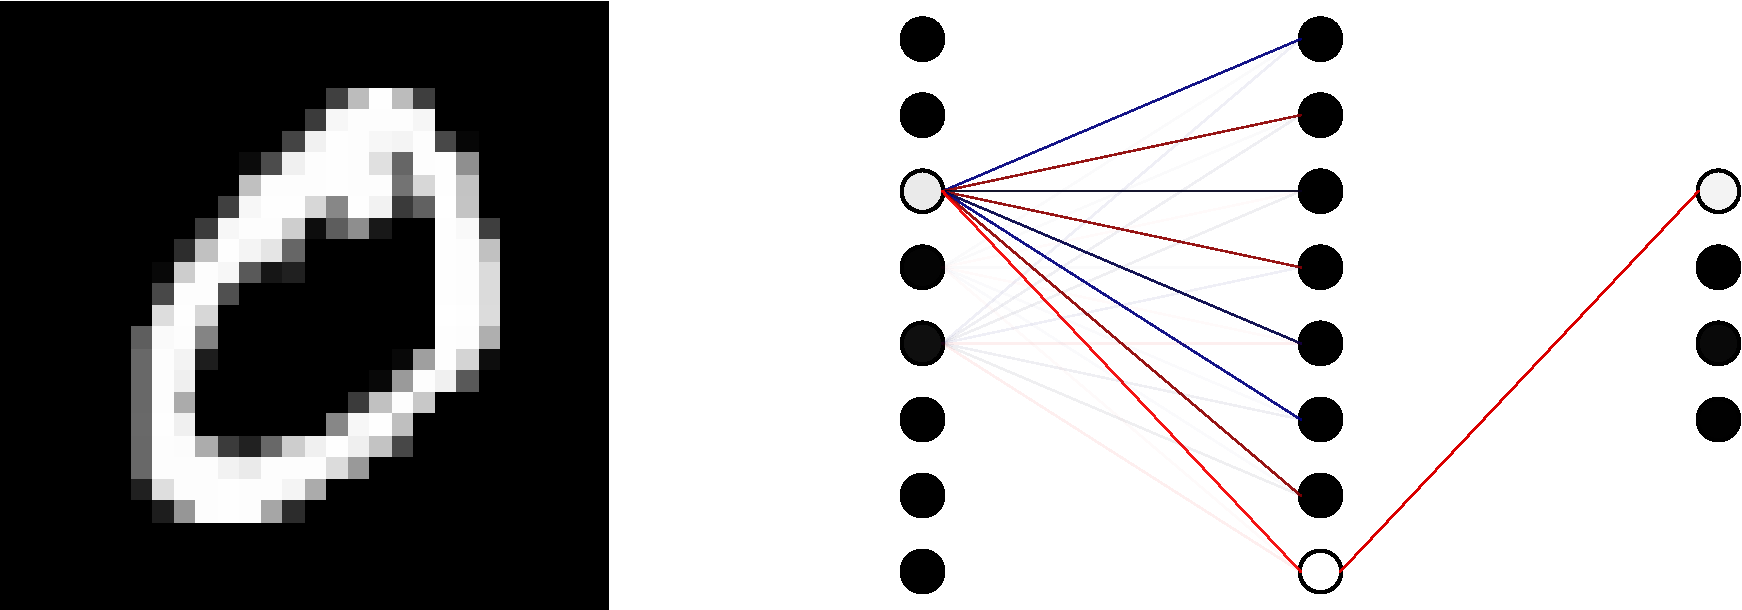
\includegraphics[width=0.9\textwidth]{figures/backpropimg2.pdf}
		\end{figure}
	\end{columns}
	\vfill
	$$
		x_3^1 = \sigma_3\left(A_{3}^{1,1}x_2^1+A_{3}^{1,2}x_2^2 +\dots+A_{3}^{1,8}x_2^8\right)
	$$
\end{frame}
\begin{frame}
	\begin{columns}[c,onlytextwidth]
		\column{0.3\textwidth}
		Iteratively, the neural networks improves its performance.
		\column{0.7\textwidth}

		\begin{figure}
			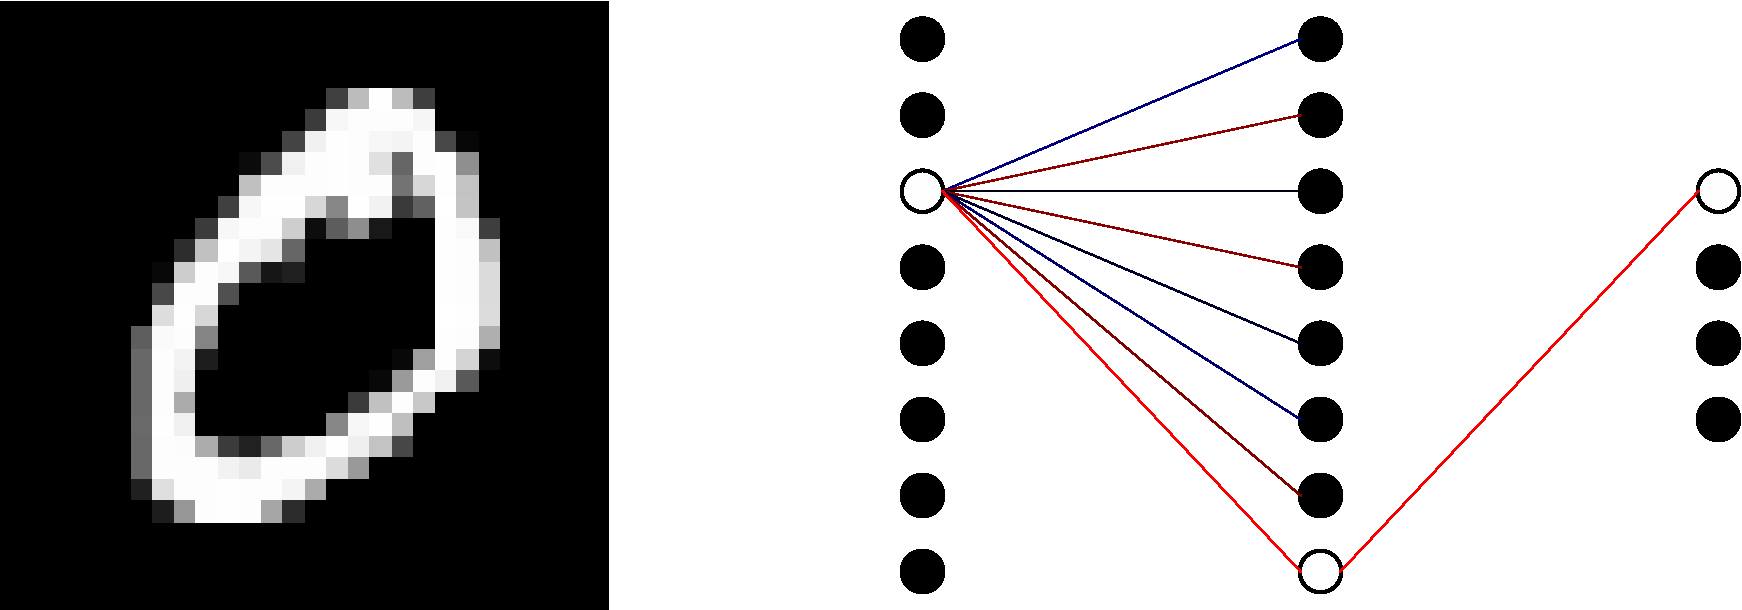
\includegraphics[width=0.9\textwidth]{figures/backpropimg3.pdf}
		\end{figure}
	\end{columns}
	\vfill
	$$
		x_3^1 = \sigma_3\left(A_{3}^{1,1}x_2^1+A_{3}^{1,2}x_2^2 +\dots+A_{3}^{1,8}x_2^8\right)
	$$
\end{frame}
\begin{frame}{}{Last Layer}
	\begin{columns}[c,onlytextwidth]
		\column{0.3\textwidth}
		We can plot the current state of the network for a given input.\newline

		Red lines show  positive values of $A_i$, Blue lines represent negative values of $A_i$.
		The level of transparency is proportional to the previous neurons.
		\column{0.7\textwidth}

		\begin{figure}
			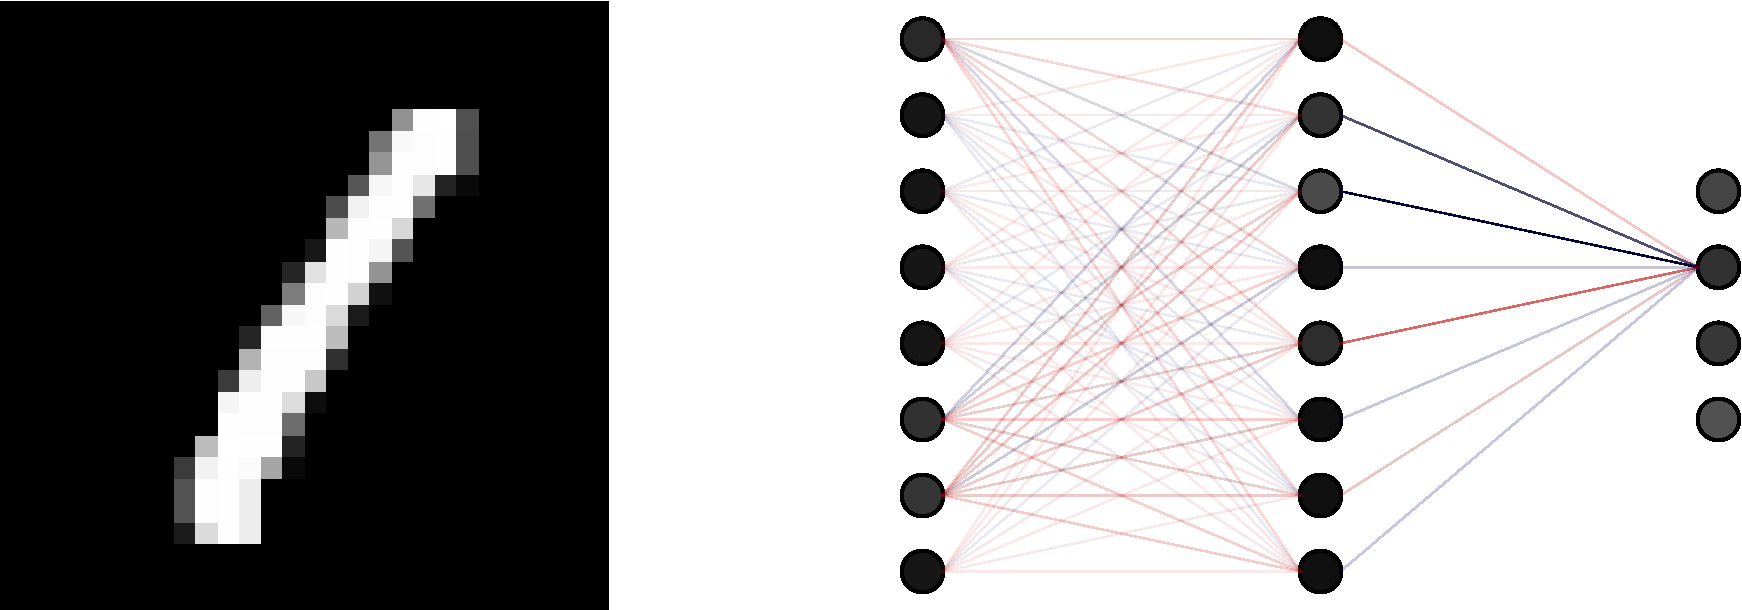
\includegraphics[width=0.9\textwidth]{figures/backpropimg01.pdf}
		\end{figure}
	\end{columns}
	\vfill
	$$
		x_3^2 = \sigma_3\left(A_{3}^{2,1}x_2^1+A_{3}^{2,2}x_2^2 +\dots+A_{3}^{2,8}x_2^8\right)
	$$
\end{frame}
\begin{frame}
	\begin{columns}[c,onlytextwidth]
		\column{0.3\textwidth}
		Iteratively, the neural networks improves its performance.
		\column{0.7\textwidth}

		\begin{figure}
			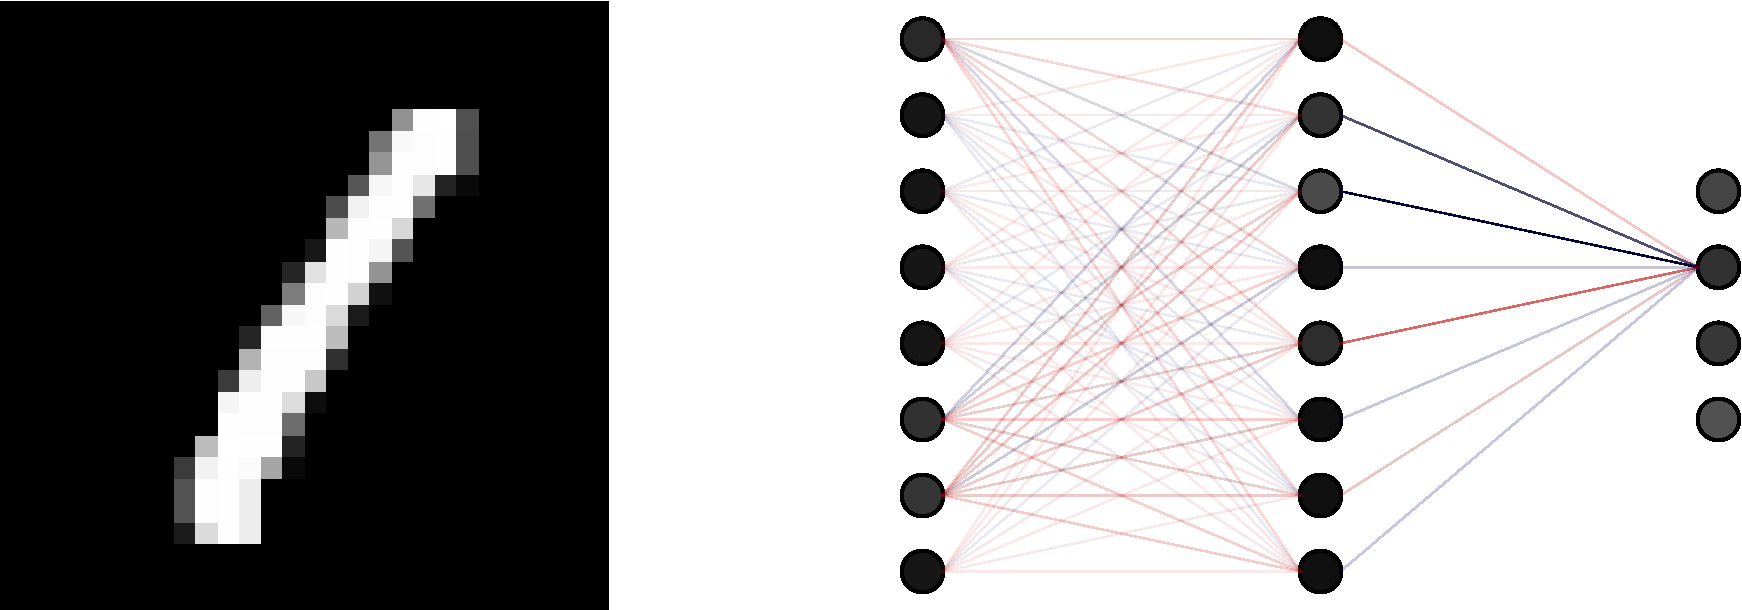
\includegraphics[width=0.9\textwidth]{figures/backpropimg01.pdf}
		\end{figure}
	\end{columns}
	\vfill
	$$
		x_3^2 = \sigma_3\left(A_{3}^{2,1}x_2^1+A_{3}^{2,2}x_2^2 +\dots+A_{3}^{2,8}x_2^8\right)
	$$
\end{frame}

\begin{frame}
	\begin{columns}[c,onlytextwidth]
		\column{0.3\textwidth}
		Iteratively, the neural networks improves its performance.
		\column{0.7\textwidth}

		\begin{figure}
			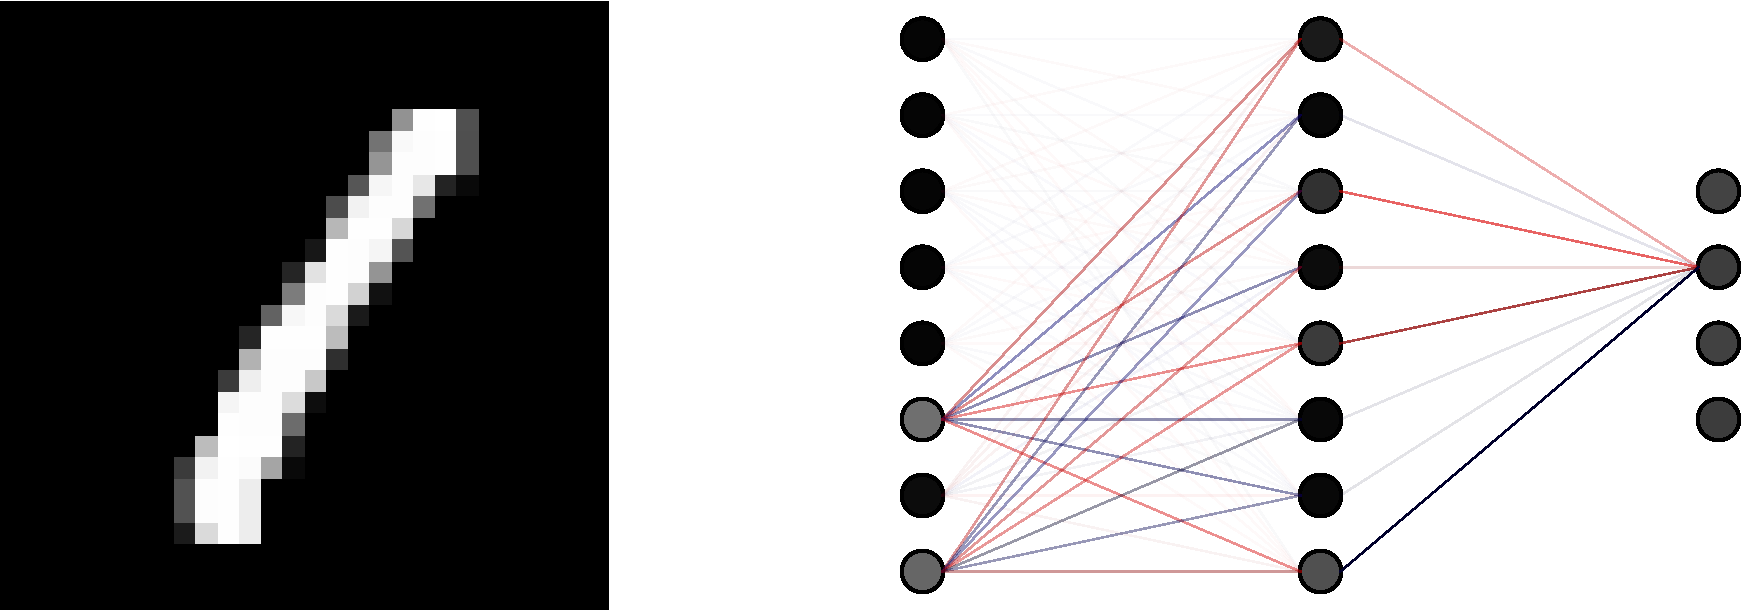
\includegraphics[width=0.9\textwidth]{figures/backpropimg11.pdf}
		\end{figure}
	\end{columns}
	\vfill
	$$
		x_3^2 = \sigma_3\left(A_{3}^{2,1}x_2^1+A_{3}^{2,2}x_2^2 +\dots+A_{3}^{2,8}x_2^8\right)
	$$
\end{frame}
\begin{frame}
	\begin{columns}[c,onlytextwidth]
		\column{0.3\textwidth}
		Iteratively, the neural networks improves its performance.
		\column{0.7\textwidth}

		\begin{figure}
			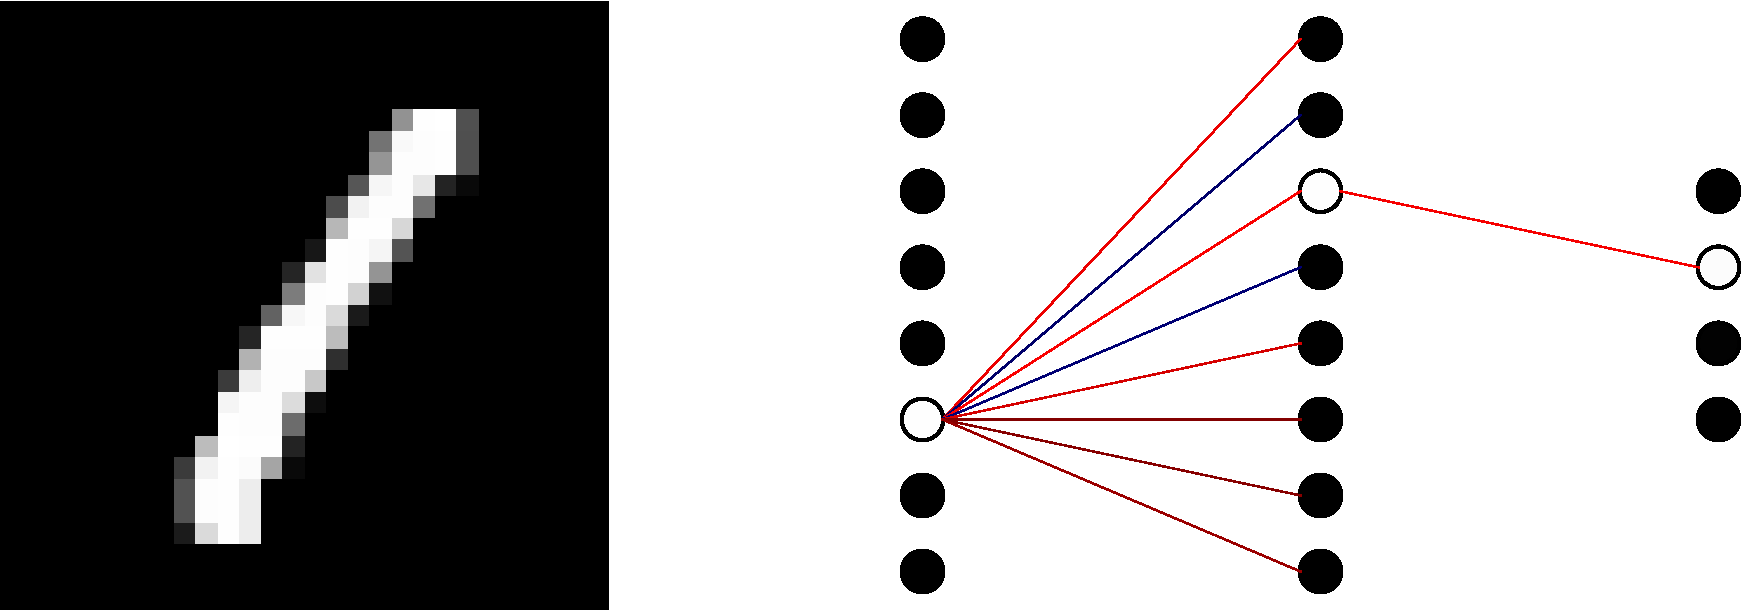
\includegraphics[width=0.9\textwidth]{figures/backpropimg13.pdf}
		\end{figure}
	\end{columns}
	\vfill
	$$
		x_3^2 = \sigma_3\left(A_{3}^{2,1}x_2^1+A_{3}^{2,2}x_2^2 +\dots+A_{3}^{2,8}x_2^8\right)
	$$
\end{frame}
\begin{frame}
	\begin{columns}[c,onlytextwidth]
		\column{0.3\textwidth}
		Iteratively, the neural networks improves its performance.
		\column{0.7\textwidth}

		\begin{figure}
			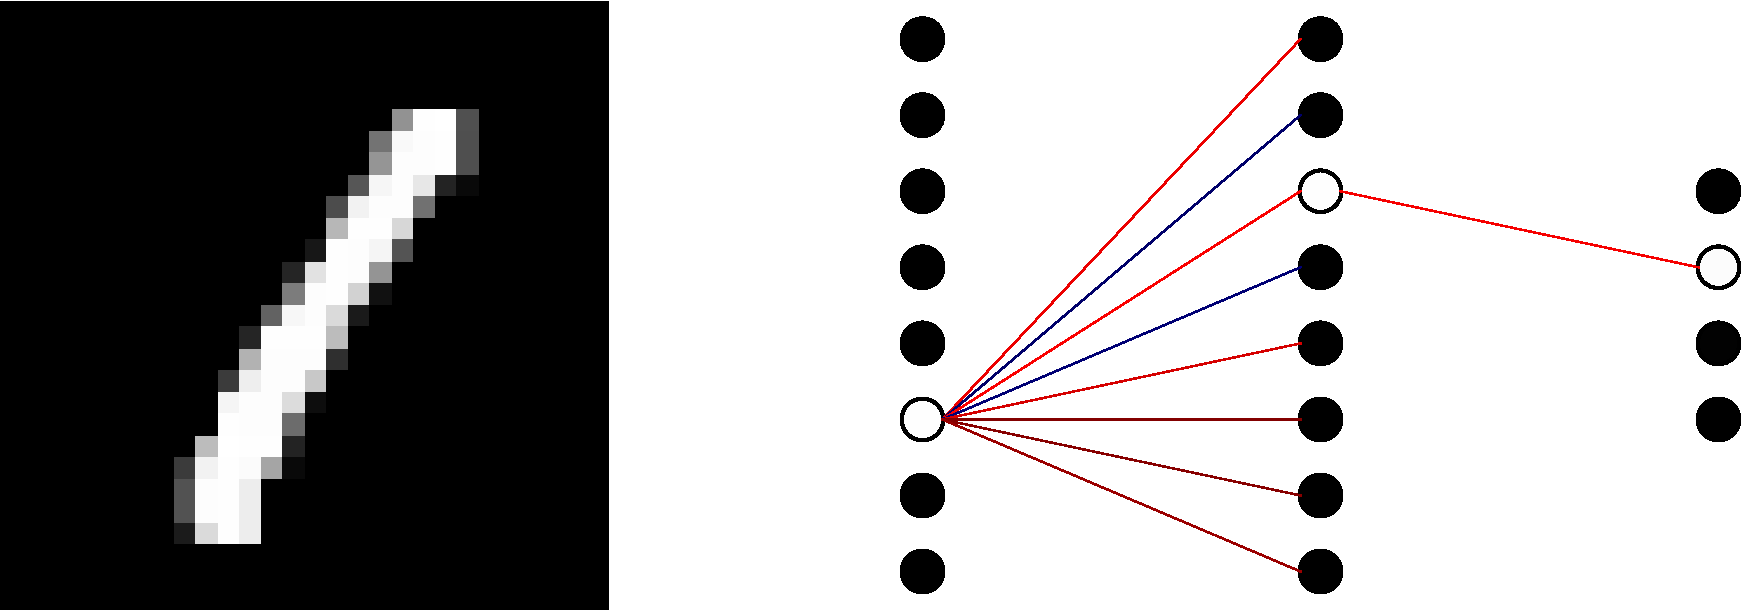
\includegraphics[width=0.9\textwidth]{figures/backpropimg13.pdf}
		\end{figure}
	\end{columns}
	\vfill
	$$
		x_3^2 = \sigma_3\left(A_{3}^{2,1}x_2^1+A_{3}^{2,2}x_2^2 +\dots+A_{3}^{2,8}x_2^8\right)
	$$
\end{frame}


\subsection{Example : Image classification of handwritten digits from A to Z}

\begin{frame}
	Having discussed the theory behind Artificial Neural Networks and the training process, we will now proceed to demonstrate a comprehensive end-to-end example of image classification on MNIST.
	\vskip 0.5cm
	\begin{figure}
		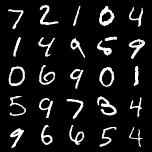
\includegraphics[width=0.4\textwidth]{figures/MNIST_full_dense.png}
	\end{figure}
\end{frame}

\begin{frame}
	\begin{itemize}
		\item Input shape : $1 \times 28 \times28$.
		\item Number of Classes : $10$.
		\item Number of training samples $(x, y)$: $60000$.
		\item Number of evaluating samples: $10000$.
		\item Loss : cross-entropy
		      $$L(\hat{y}, y) = - \frac{1}{N} \sum_{i=1}^{N} \sum_{j=1}^{K} y_{ij} \log(\hat{y}_{ij})$$
		      where :
		      \begin{itemize}
			      \item $\hat{y} \in \mathbb{R}^{N \times K}$ is the predicted probability distribution over $K$ classes for $N$ samples,
			      \item $y \in {0,1}^{N \times K}$ is the ground-truth one-hot encoded label matrix,
		      \end{itemize}
	\end{itemize}
\end{frame}

\begin{frame}{Recap on the Cross-Entropy Loss}

	\begin{tikzpicture}
		% One-hot distribution
		\begin{axis}[
				title={One-Hot Distribution ($y_i$)},
				height=6cm, width=9cm,
				symbolic x coords={Class 1, Class 2, Class 3, Class 4, Class 5},
				xtick=data,
				ymin=0, ymax=1,
				ytick={0, 0.2, 0.4, 0.6, 0.8, 1},
				bar width=0.6cm,
				nodes near coords,
				enlarge x limits=0.3,
				grid=major,
				ticklabel style={font=\footnotesize}
			]
			\addplot[ybar,fill=primary] coordinates {
					(Class 1, 0)
					(Class 2, 0)
					(Class 3, 1)
					(Class 4, 0)
					(Class 5, 0)
				};
		\end{axis}
	\end{tikzpicture}
	\hfill
	\begin{tikzpicture}
		% Model predicted distribution
		\begin{axis}[
				title={Model Predicted Distribution ($\hat{y}_i$)},
				height=6cm, width=9cm,
				symbolic x coords={Class 1, Class 2, Class 3, Class 4, Class 5},
				xtick=data,
				ymin=0, ymax=1,
				ytick={0, 0.2, 0.4, 0.6, 0.8, 1},
				bar width=0.6cm,
				nodes near coords,
				enlarge x limits=0.3,
				grid=major,
				ticklabel style={font=\footnotesize}
			]
			\addplot[ybar,fill=secondary] coordinates {
					(Class 1, 0.1)
					(Class 2, 0.15)
					(Class 3, 0.5)
					(Class 4, 0.2)
					(Class 5, 0.05)
				};
		\end{axis}
	\end{tikzpicture}

	The cross-entropy loss for one sample is:
	$$
		l(\hat{y}_i, y_i) = -  \sum_{j=1}^{K} y_{ij} \log(\hat{y}_{ij}).
	$$

\end{frame}

\begin{frame}
	We build a 3 layers network.
	\begin{itemize}
		\item Batch size : 64
		\item Learning rate : 0.01
		\item Intermediate activation : ReLU
		\item Final activation : Softmax
		\item Number of epochs : 12
		      % \item Scheduler : we divide $\lambda$ by $2$ every 3 epochs.
		\item Number of trained parameters: $52.6$k
	\end{itemize}

	\begin{figure}
		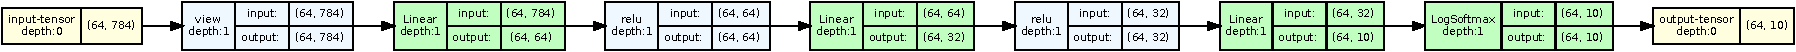
\includegraphics[width=\textwidth]{figures/densemnist.pdf}
	\end{figure}
\end{frame}
\begin{frame}
	\begin{figure}
		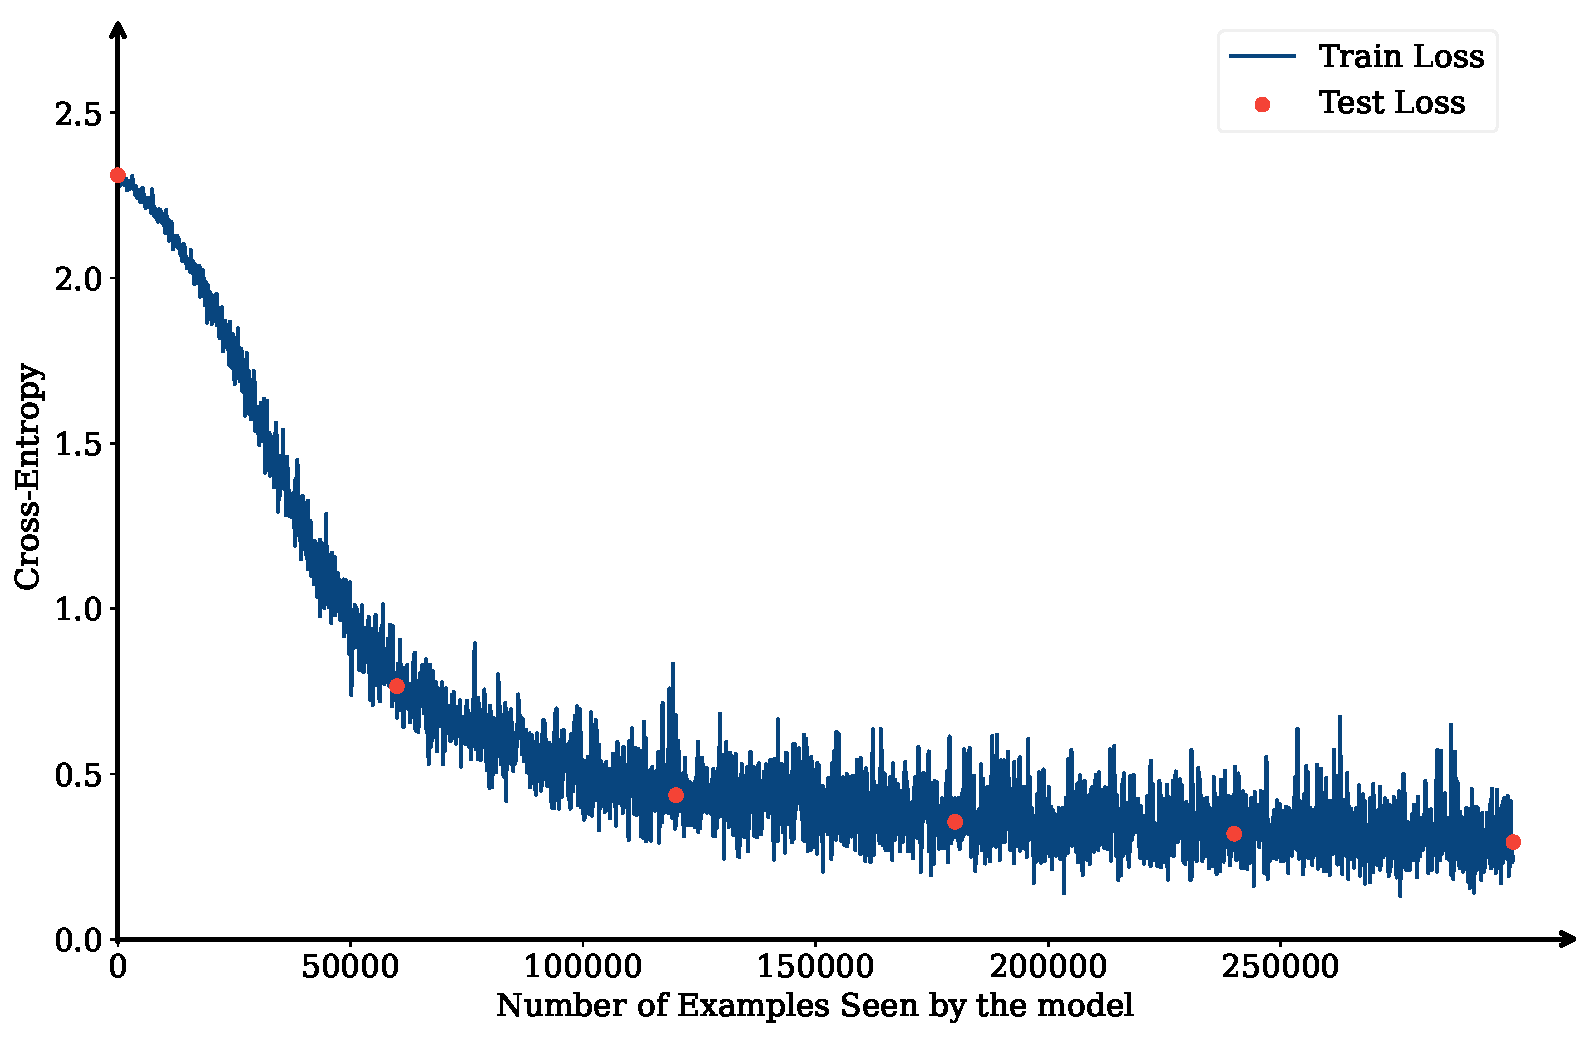
\includegraphics[width=0.7\textwidth]{figures/densemnist_res.pdf}
	\end{figure}
\end{frame}
% \begin{frame}
% 	With an interpretation tool such as SHAP:
% 	\begin{figure}
% 		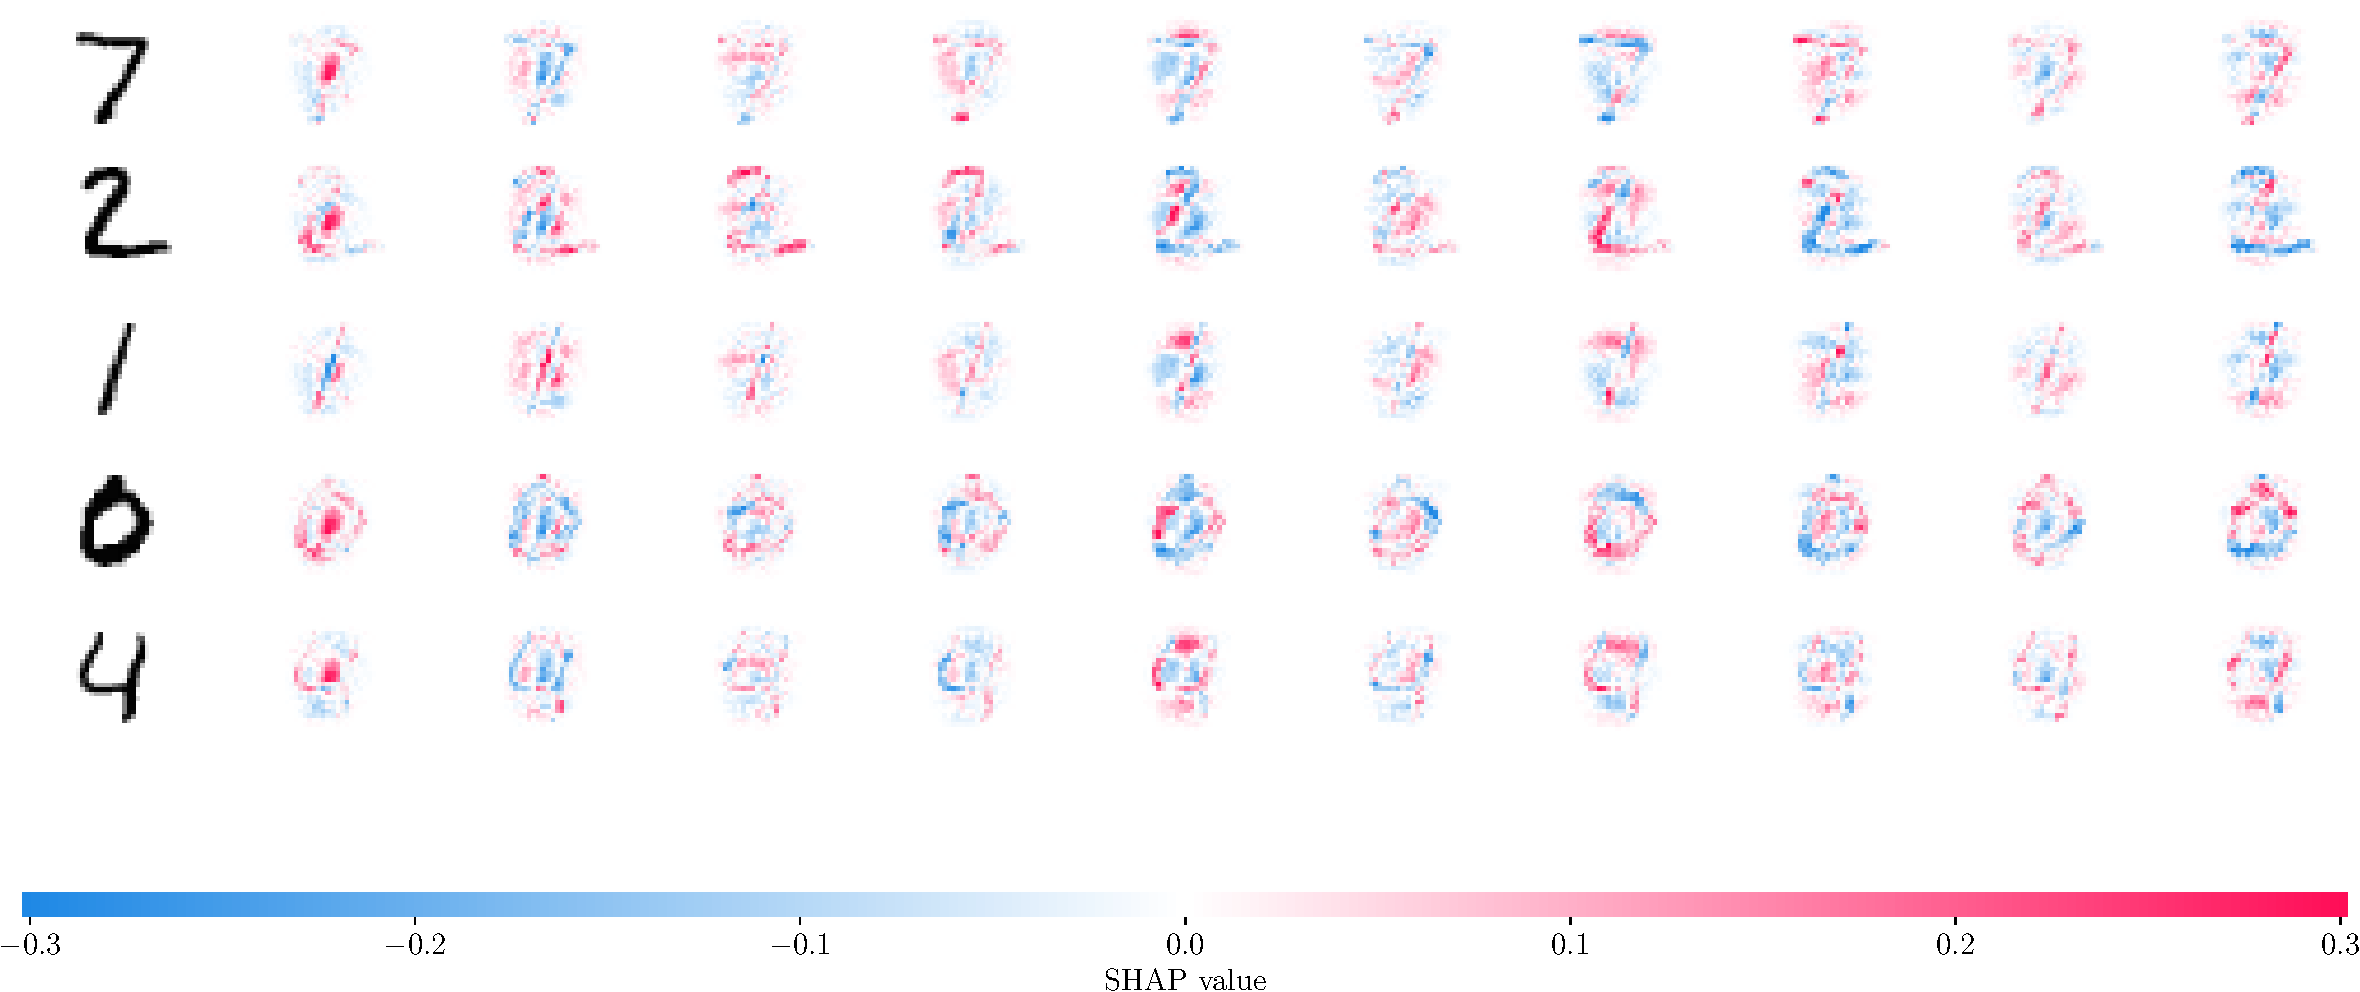
\includegraphics[width=1\textwidth]{figures/shapdense.pdf}
% 	\end{figure}
% \end{frame}

\begin{frame}{The Multi-layer Perceptron (MLP)}{The first Deep Learning Model}
	Link to the notebook: \href{
		https://lamsade.dauphine.fr/~averine/EM_IASD/TP1.ipynb}{Notebook Collab}\\
	Link to the notebook: \href{https://lamsade.dauphine.fr/~averine/EM_IASD/TP1.html}{html}
\end{frame}

\begin{frame}{}{Your turn !}
	Get the Notebook on the course website and start working on it.
	\begin{itemize}
		\item \url{https://www.alexverine.com}
		\item Teaching
		\item Introduction to Deep Learning
		\item Lien Notebook
	\end{itemize}
	During this hands-on session we get you started with the basics of deep learning using PyTorch. You will implement a simple feedforward neural network (Multi-Layer Perceptron) to classify handwritten digits from the MNIST dataset.
\end{frame}


\makepart{Deep Learning in Action: From Neural Networks to Transformer Models}


\begin{frame}
	Now that we have an understanding of the training procedure for Artificial Neural Networks, we shall examine several widely-utilized structures within the literature of Neural Networks, including Convolutional Neural Networks (CNN),Resdiual Networks (ResNet),  Recurrent Neural Networks (RNN), and Transformers.
\end{frame}

\section{Convolutional Neural Networks}
\begin{frame}
	In the field of image processing, the Convolution Operators are widely considered as the most favoured approach. While it has been demonstrated that Dense blocks, or Linear blocks, are capable of accurately classifying images in the case of the MNIST dataset, the need for convolutional transformations arises when addressing wider and more intricate datasets.
\end{frame}
\subsection{The Two dimensional Convolution}
\begin{frame}
	A 2D convolution in a neural network context can be mathematically represented as a sliding window operation where a filter (also called kernel) $w$ of size $k \times k$ is applied to each $k \times k$ sub-matrix of the input matrix $x$. The operation can be defined as the element-wise multiplication of the filter $w$ and the sub-matrix followed by summing the results, i.e.

	$$y_{i,j} = \sum\limits_{m=1}^{k} \sum\limits_{n}^{k} w_{m,n} \cdot x_{i+m, j+n}$$

	\begin{figure}
		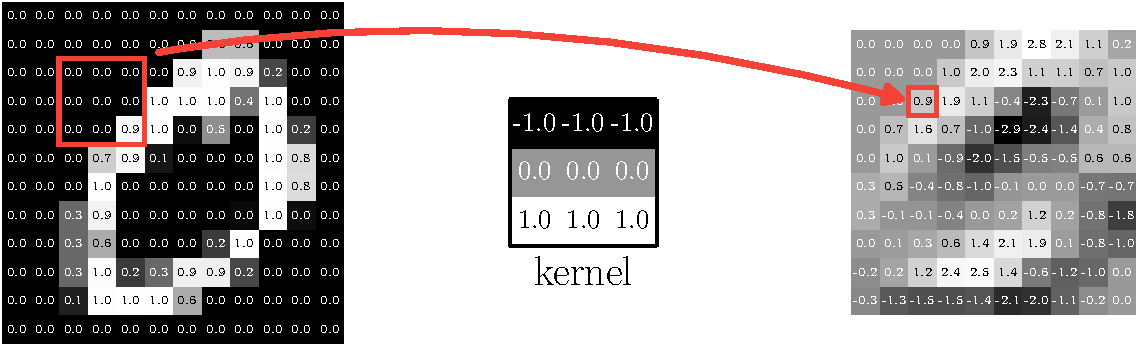
\includegraphics[width=0.6\textwidth]{figures/conv1.pdf}
	\end{figure}
\end{frame}


\begin{frame}
	A 2D convolution in a neural network context can be mathematically represented as a sliding window operation where a filter (also called kernel) $w$ of size $k \times k$ is applied to each $k \times k$ submatrix of the input matrix $x$. The operation can be defined as the element-wise multiplication of the filter $w$ and the submatrix followed by summing the results, i.e.

	$$y_{i,j} = \sum\limits_{m=1}^{k} \sum\limits_{n}^{k} w_{m,n} \cdot x_{i+m, j+n}$$

	\begin{figure}
		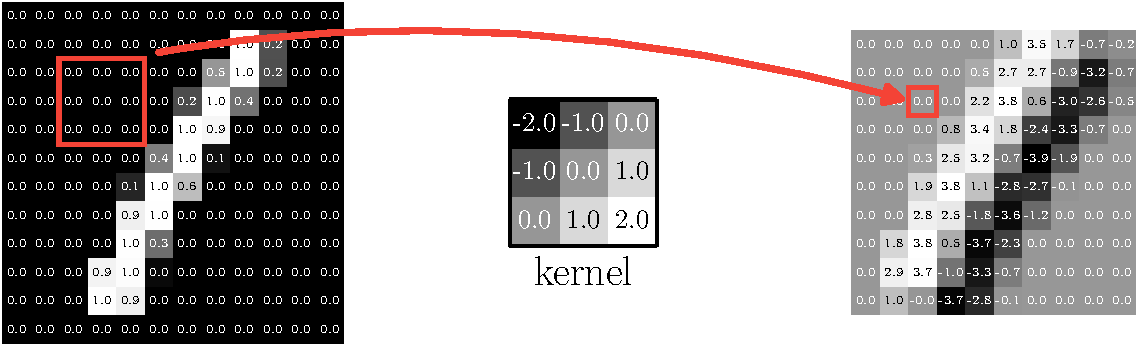
\includegraphics[width=0.6\textwidth]{figures/conv2.pdf}
	\end{figure}
\end{frame}
\begin{frame}{}{Kernel Size, Padding and  Stride}
	In every Deep Learning library, the Conv2D block takes three parameters in argument:
	\begin{itemize}
		\item the Kernel's size,
		\item the Stride,
		\item the Padding.
	\end{itemize}
	The size out the output is :
	$$
		d_{\mathrm{out}} = \frac{d_{\mathrm{in}}+2\times \mathrm{Padding}  - \mathrm{Kernel Size}  }{\mathrm{Stride}}+1
	$$
\end{frame}

\begin{frame}{}{Kernel Size, Padding and  Stride}
	Kernel size: $3$, Padding: $0$, Stride: $1$
	\begin{figure}
		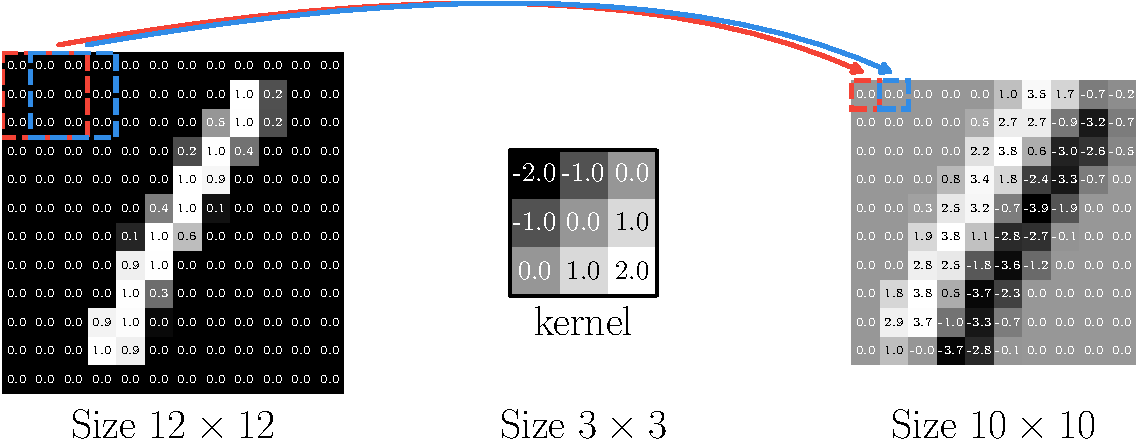
\includegraphics[width = 0.7 \textwidth]{figures/convk3.pdf}
	\end{figure}
	\vfill
	$$
		d_{\mathrm{out}} = \frac{d_{\mathrm{in}}+2\times \mathrm{Padding}  - \mathrm{Kernel Size}  }{\mathrm{Stride}}+1
	$$
\end{frame}

\begin{frame}{}{Kernel Size, Padding and  Stride}
	Kernel size: $5$, Padding: $0$, Stride: $1$
	\begin{figure}
		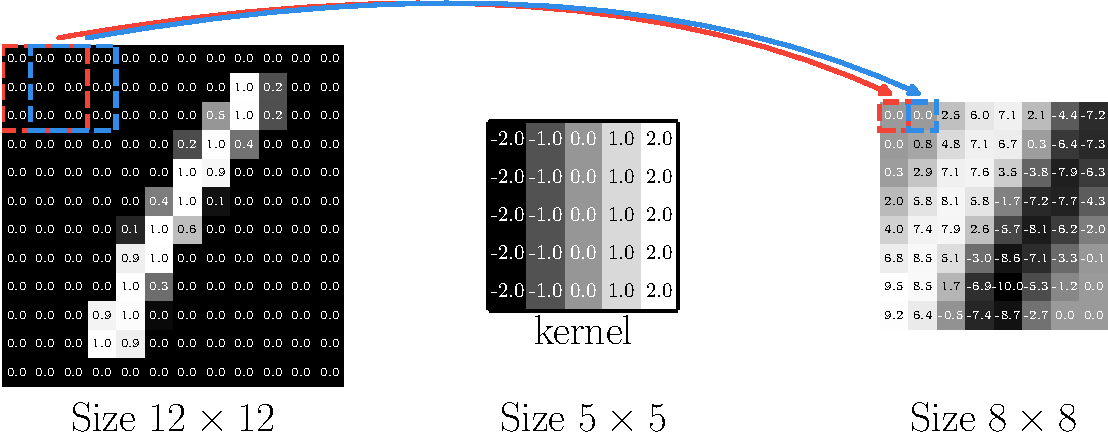
\includegraphics[width = 0.7 \textwidth]{figures/convk5.pdf}
	\end{figure}
	\vfill
	$$
		d_{\mathrm{out}} = \frac{d_{\mathrm{in}}+2\times \mathrm{Padding}  - \mathrm{Kernel Size}  }{\mathrm{Stride}}+1
	$$
\end{frame}

\begin{frame}{}{Kernel Size, Padding and  Stride}
	Kernel size: $3$, Padding: $1$, Stride: $1$. Padding mode can be 'zeros', 'reflect', 'replicate' or 'circular'.
	\begin{figure}
		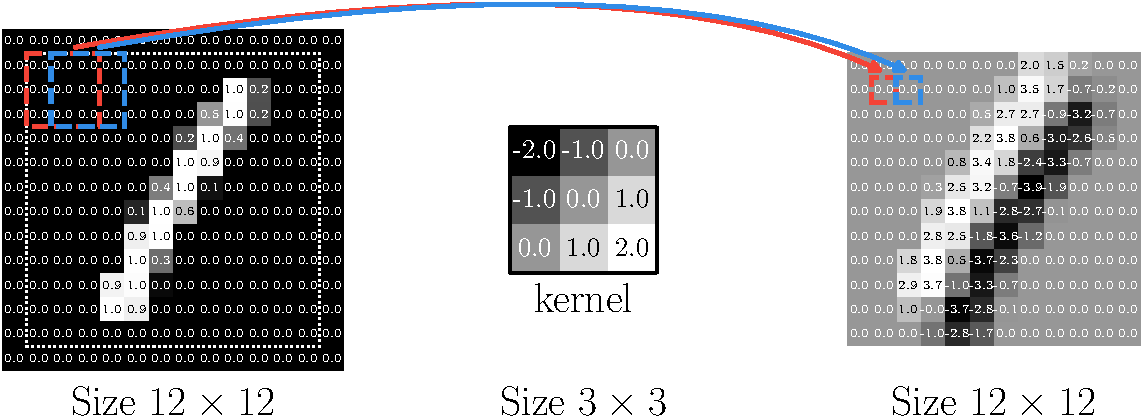
\includegraphics[width = 0.7 \textwidth]{figures/convp1.pdf}
	\end{figure}
	\vfill
	$$
		d_{\mathrm{out}} = \frac{d_{\mathrm{in}}+2\times \mathrm{Padding}  - \mathrm{Kernel Size}  }{\mathrm{Stride}}+1
	$$
\end{frame}

\begin{frame}{}{Kernel Size, Padding and  Stride}
	Kernel size: $3$, Padding: $1$, Stride: $2$
	\begin{figure}
		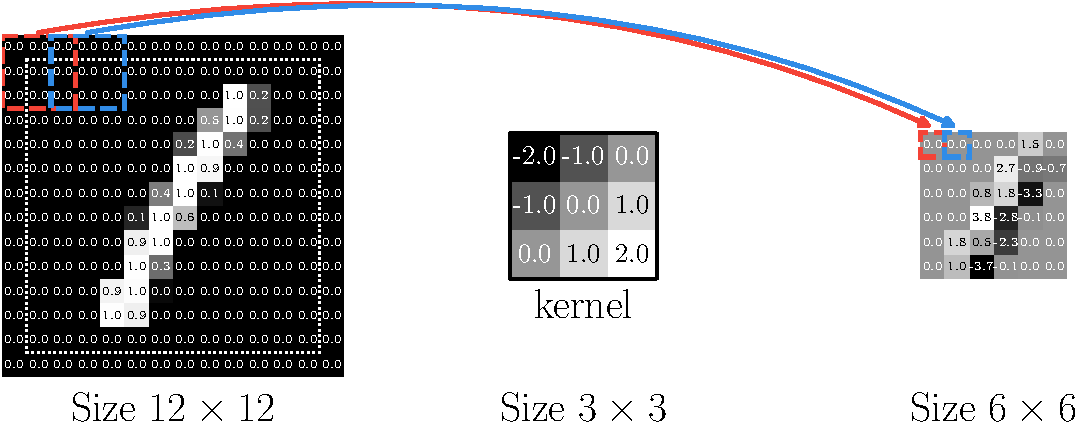
\includegraphics[width = 0.7 \textwidth]{figures/convs2.pdf}
	\end{figure}
	\vfill
	$$
		d_{\mathrm{out}} = \frac{d_{\mathrm{in}}+2\times \mathrm{Padding}  - \mathrm{Kernel Size}  }{\mathrm{Stride}}+1
	$$
\end{frame}

\begin{frame}{}{Kernel Size, Padding and  Stride}
	Kernel size: $3$, Padding: $1$, Stride: $3$
	\begin{figure}
		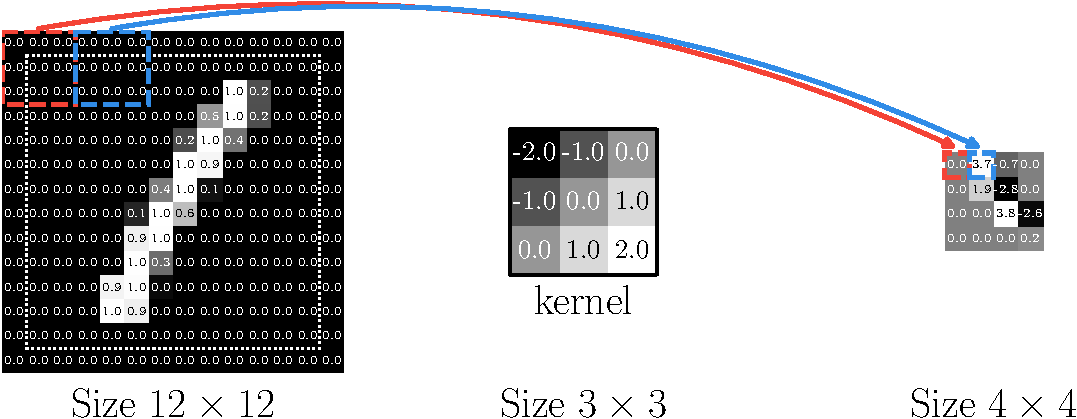
\includegraphics[width = 0.7 \textwidth]{figures/convs3.pdf}
	\end{figure}
	\vfill
	$$
		d_{\mathrm{out}} = \frac{d_{\mathrm{in}}+2\times \mathrm{Padding}  - \mathrm{Kernel Size}  }{\mathrm{Stride}}+1
	$$
\end{frame}

\subsection{CNN : Convolutional in a network Networks}
\begin{frame}
	We can  represent a CNN as under this form:

	\begin{figure}
		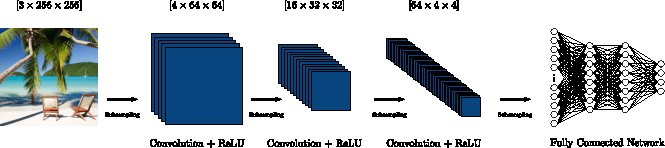
\includegraphics[width=1\textwidth]{figures/conv.pdf}
	\end{figure}
\end{frame}

\begin{frame}
	Usually, the output of a convolutional block is linear combination of the Convolutional output of every previous channels and a bias:
	$$
		\mathrm{out}_{i,j}(c_\mathrm{out}) = \mathrm{bias}(c_\mathrm{out}) + \sum_{k=0}^{\vert c_{\mathrm{in}} \vert-1} \mathrm{Conv}(\mathrm{input}(k), \mathrm{kernel}_k )_{i,j}
	$$

	\begin{figure}
		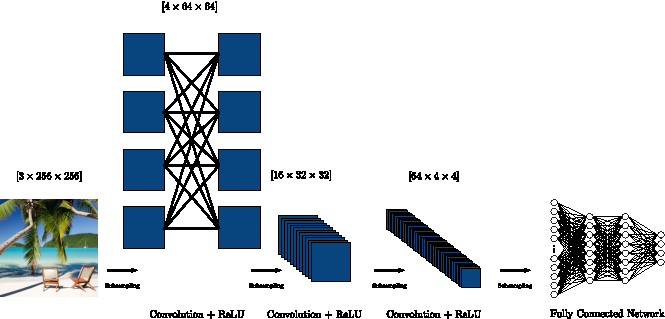
\includegraphics[width=0.7\textwidth]{figures/convfc1.pdf}
	\end{figure}

\end{frame}

\begin{frame}
	In practice, we split the image into multiple channels : the three channels RGB to begin with. Then we apply convolutional operation on different scales and then we use a fully connected tail. To change the scale we can use different sub-sampling : Max pooling, Average pooling or Invertible pooling.

	\begin{figure}
		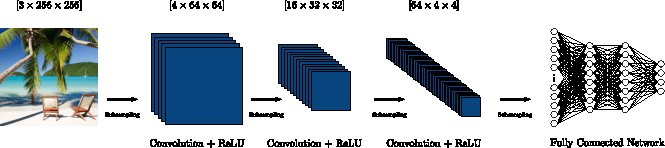
\includegraphics[width=1\textwidth]{figures/conv.pdf}
	\end{figure}
\end{frame}

\begin{frame}{}{Max Pooling}
	Max Pooling take the maximum within a given sized sub-matrix. In practice, the matrix is size $2\times 2$ in order to reduce the dimension by $4$ and doubling the scale.

	\begin{figure}
		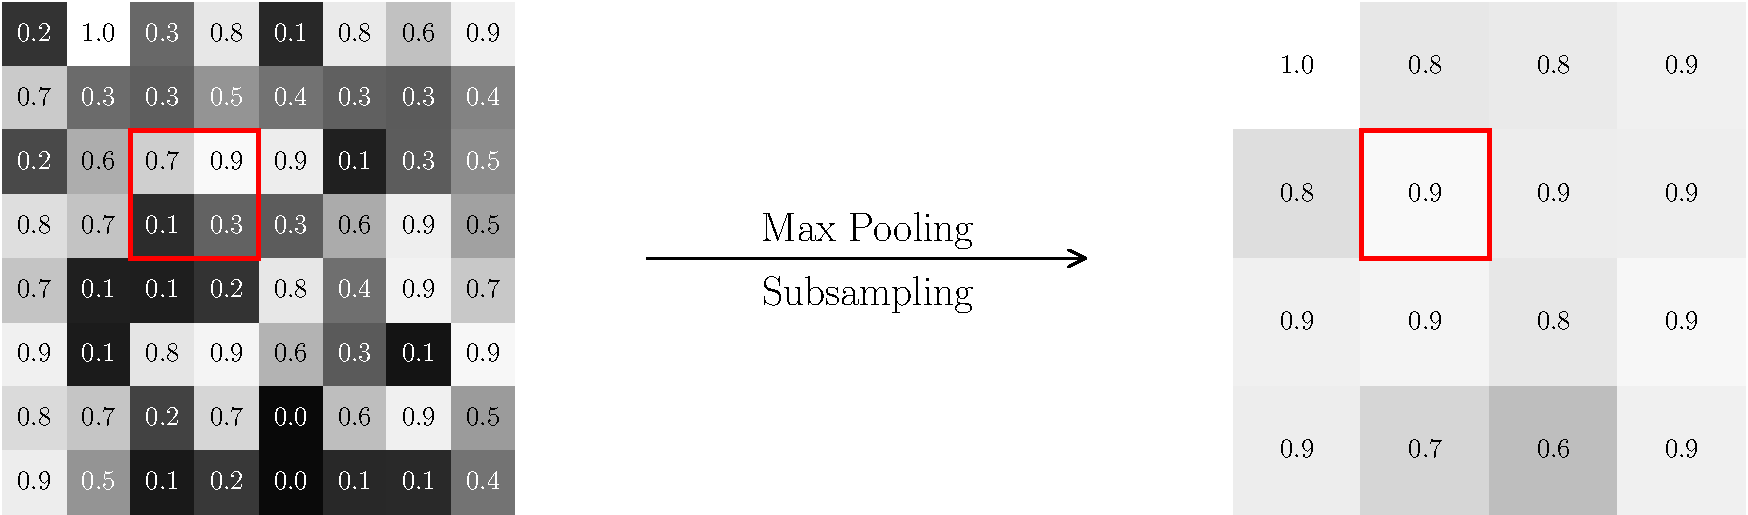
\includegraphics[width=1\textwidth]{figures/maxpooling.pdf}
	\end{figure}
\end{frame}


\begin{frame}{}{Average Pooling}
	The Average pooling takes the average value within the sub-matrix.

	\begin{figure}
		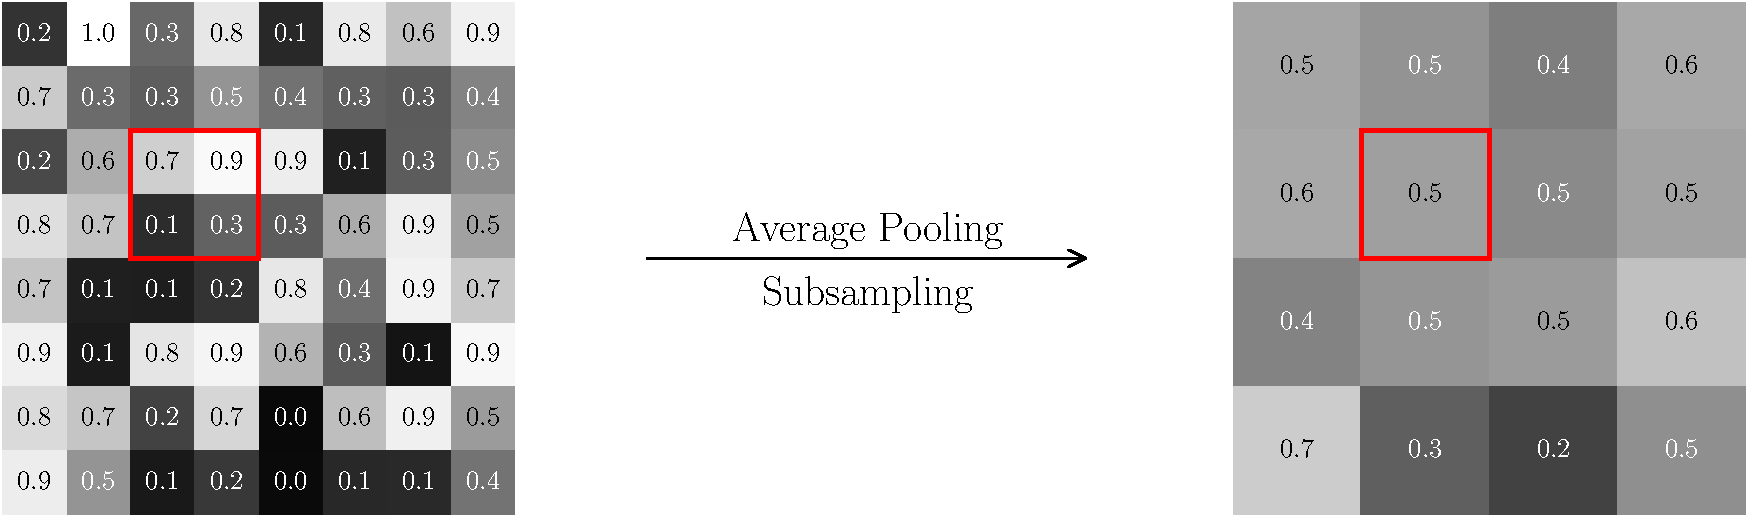
\includegraphics[width=1\textwidth]{figures/avgpooling.pdf}
	\end{figure}
\end{frame}


\begin{frame}{}{Invertible Pooling}
	For Invertible Networks, we can use Invertible Pooling, aka Squeeze. It preserves the information contained in the channels and keeps the dimension constant.

	\begin{figure}
		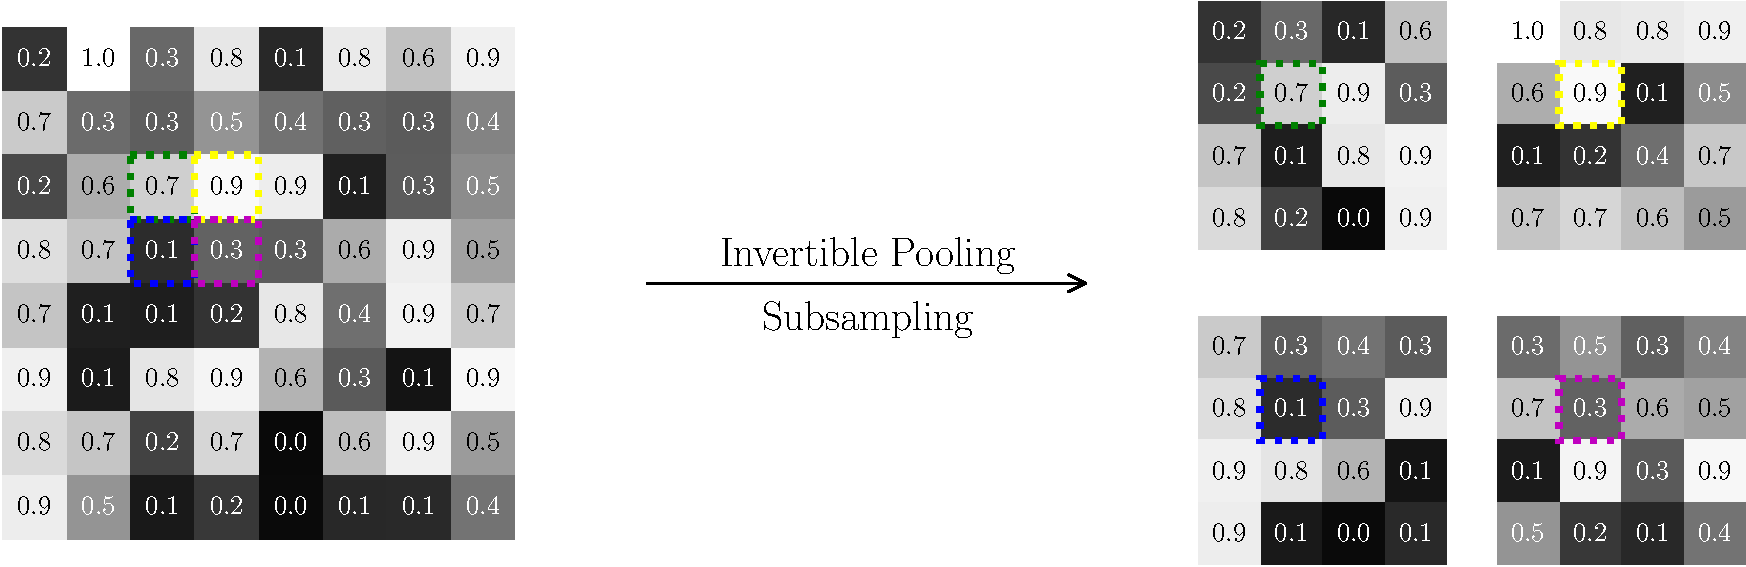
\includegraphics[width=1\textwidth]{figures/squeezepooling.pdf}
	\end{figure}
\end{frame}


\begin{frame}
	Convolutional Neural Networks are more suitable for image processing compared to fully connected networks due to their ability to efficiently handle the spatial relationships between pixels in an image. This is achieved through the use of convolutional layers that apply filters to small portions of an image, rather than fully connected layers that process the entire image as a single vector. Additionally, the shared weights in convolutional layers allow for learning of hierarchical features, reducing the number of parameters in the network and increasing its ability to generalize to new images.
\end{frame}

\subsection{CNN in practice: CIFAR 10}

\begin{frame}
	\begin{itemize}
		\item Input shape : $3 \times 32 \times32$.
		\item Number of Classes : $10$.
		\item Number of training samples $(x, y)$: $50000$.
		\item Number of evaluating samples: $10000$.
	\end{itemize}
	\begin{figure}
		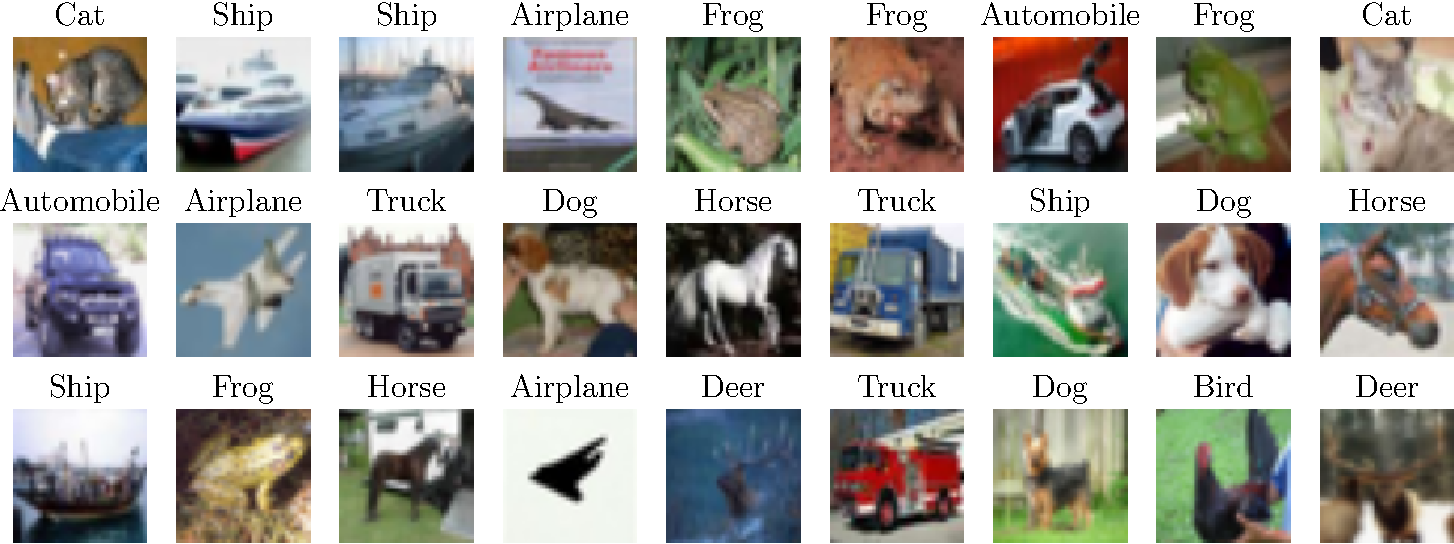
\includegraphics[width= 0.8\textwidth]{figures/cifar10.pdf}
	\end{figure}
\end{frame}
\begin{frame}
	We will compare three different models:
	\begin{itemize}

		\item Model 1 : Fully Connected Neural Network with $3.4$ million parameters.
		\item Model 2 : CNN with $62$ thousand parameters.
		\item Model 3 : Wider and longer CNN with $5.8$ million parameters.
	\end{itemize}
\end{frame}

\begin{frame}{}{Model 1 : Fully Connected Neural Network}
	The Net in composed of 4 linear layers with ReLU activations:
	\begin{itemize}
		\item Linear $3072 \mapsto 1024$ + ReLU
		\item Linear $1024 \mapsto 256$ + ReLU
		\item Linear $256 \mapsto 64$ + ReLU
		\item Linear $64 \mapsto 10$ + SoftMax
	\end{itemize}
\end{frame}

\begin{frame}{}{Model 1}
	\begin{figure}
		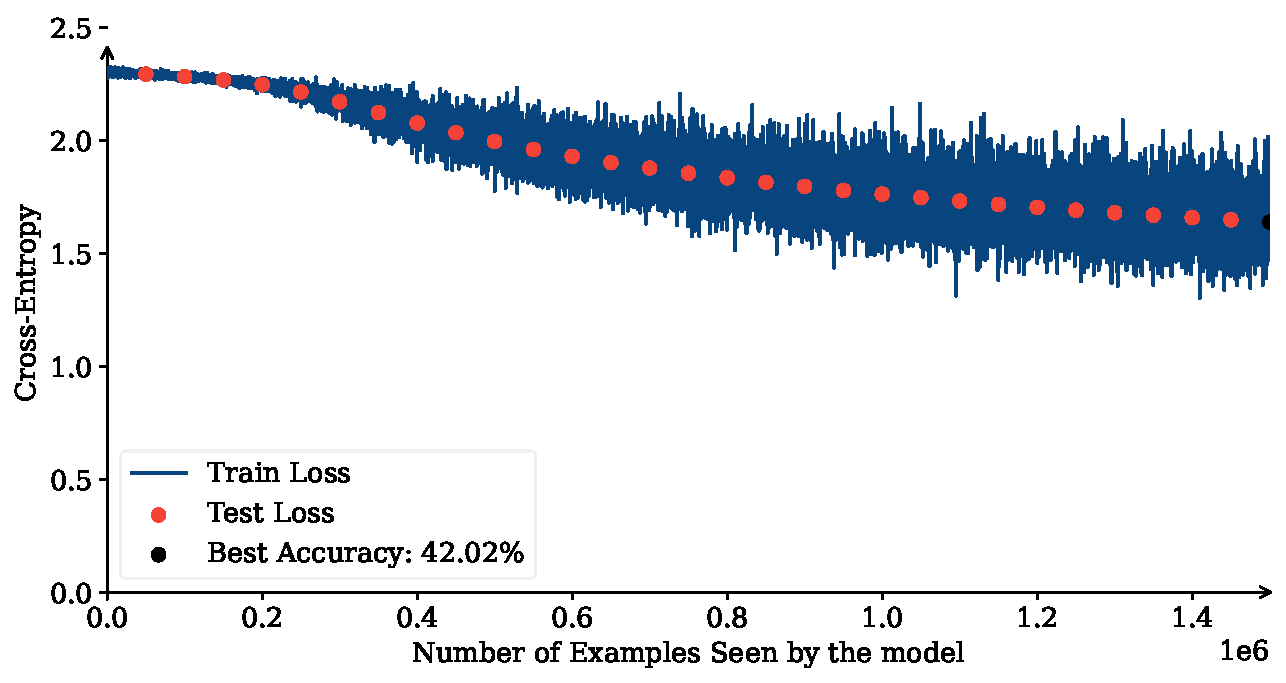
\includegraphics[width = 0.7 \textwidth]{figures/sgd_cifar_fc.pdf}
	\end{figure}
\end{frame}

\begin{frame}{}{Using a better optimization algorithm ?}
	\textbf{Adam}: Adam is an optimization algorithm that can be used instead of the classical stochastic gradient descent procedure to update network weights iteratively based on training data. It combines the advantages of two other extensions of stochastic gradient descent, AdaGrad and RMSProp, and is designed to work well for a wide range of applications:
	\begin{align*}
		\theta_{t+1} & = \theta_t - \frac{\lambda}{\sqrt{\hat{v}_t} + \varepsilon} \hat{m}_t \\
		\hat{m}_t    & = \beta_1 m_{t-1} + (1-\beta_1) \nabla_\theta l(\theta_t)             \\
		\hat{v}_t    & = \beta_2 v_{t-1} + (1-\beta_2) \nabla_\theta l(\theta_t)^2
	\end{align*}
	\begin{itemize}
		\item $\lambda$ is the learning rate.
		\item $\hat{m}_t$ is the moving average of the gradient. It allows to smooth the gradient step.
		\item By dividing the gradient by the square root of the moving average of the squared gradient, we can adapt the learning rate for each parameter to improve the convergence speed.
	\end{itemize}
\end{frame}


\begin{frame}{}{Model 1}
	\begin{figure}
		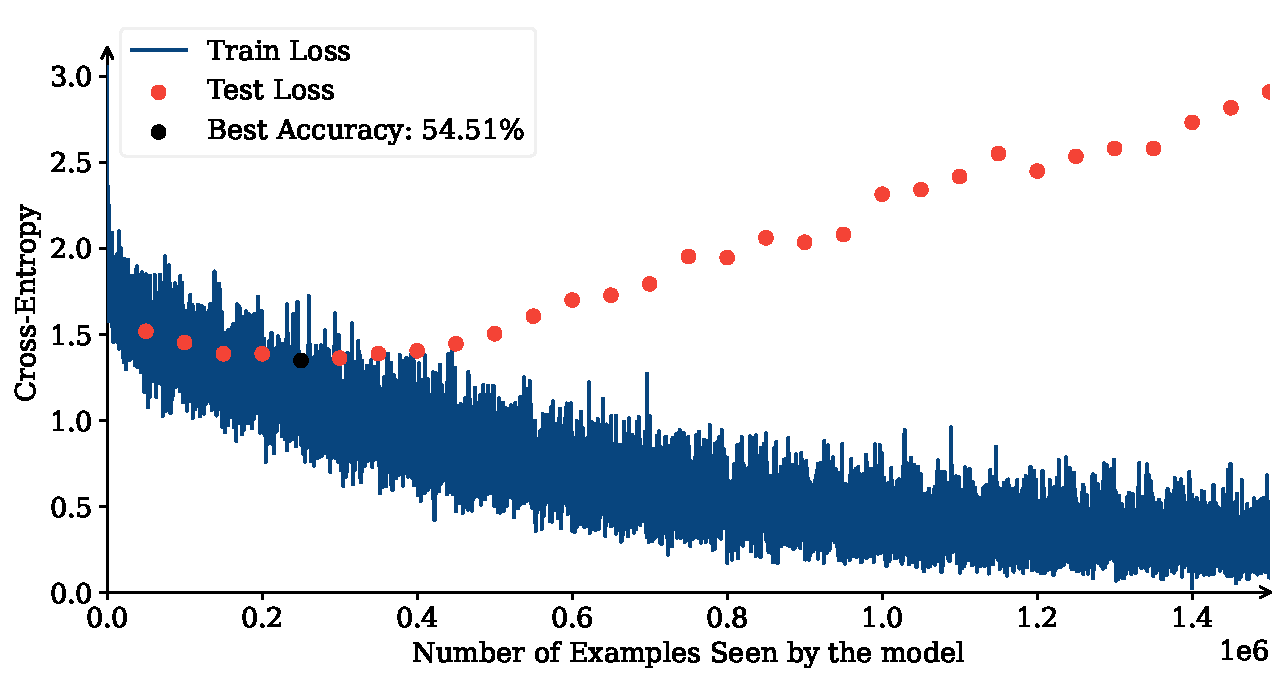
\includegraphics[width = 0.7 \textwidth]{figures/adam_cifar_fc.pdf}
	\end{figure}
\end{frame}

\begin{frame}{}{Model 1}
	\begin{figure}
		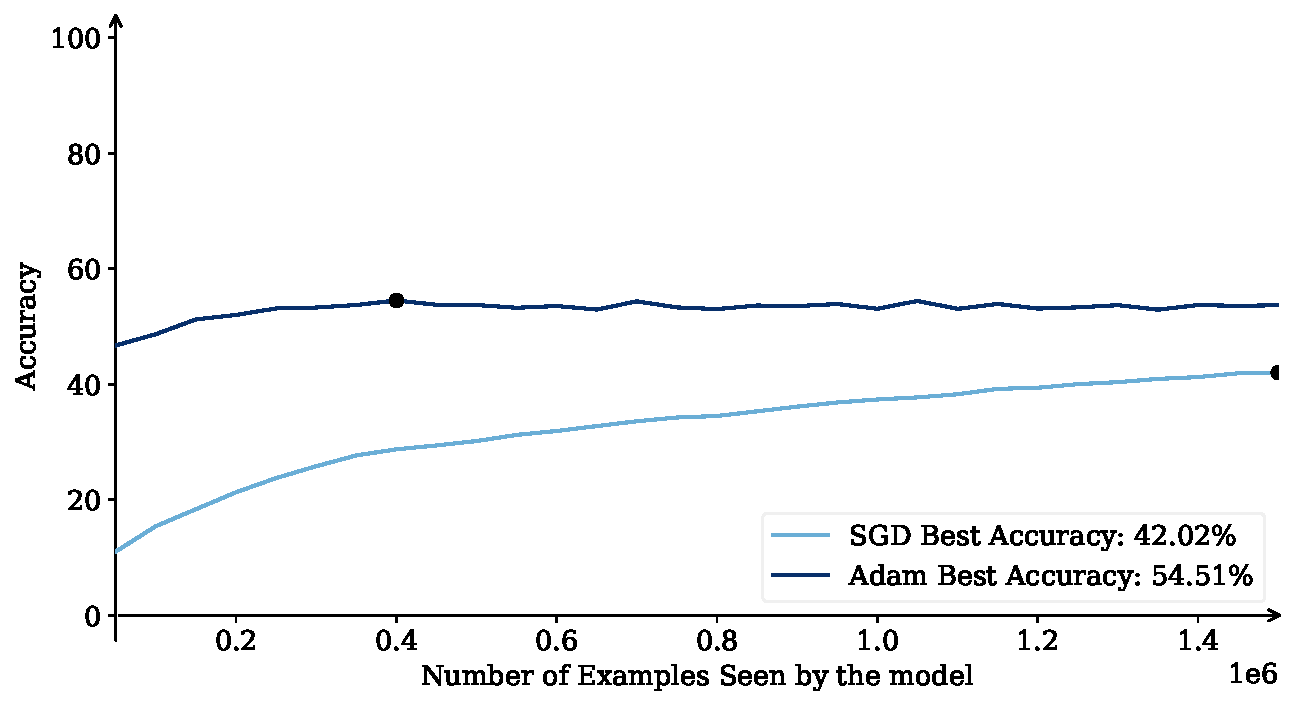
\includegraphics[width = 0.7 \textwidth]{figures/accuracies_cifar_fc.pdf}
	\end{figure}
\end{frame}

\begin{frame}{}{Model 2}
	The Net is composed 2 convolutional layers and 2 linear layers:
	\begin{itemize}
		\item Conv $3\times 32 \times 32 \mapsto 6 \times 28 \times 28$ + ReLU
		\item Max Pooling $ 6 \times 28 \times 28 \mapsto 6 \times 14 \times 14$
		\item Conv $6\times 14 \times 14 \mapsto 16 \times 10 \times 10$ + ReLU
		\item Max Pooling $ 16 \times 10 \times 10 \mapsto 16 \times 5 \times 5$
		\item Linear $400 \mapsto 120$ + ReLU
		\item Linear $120 \mapsto 84$ + ReLU
		\item Linear $84 \mapsto 10$ + SoftMax
	\end{itemize}
\end{frame}

\begin{frame}{}{Model 2}
	\begin{figure}
		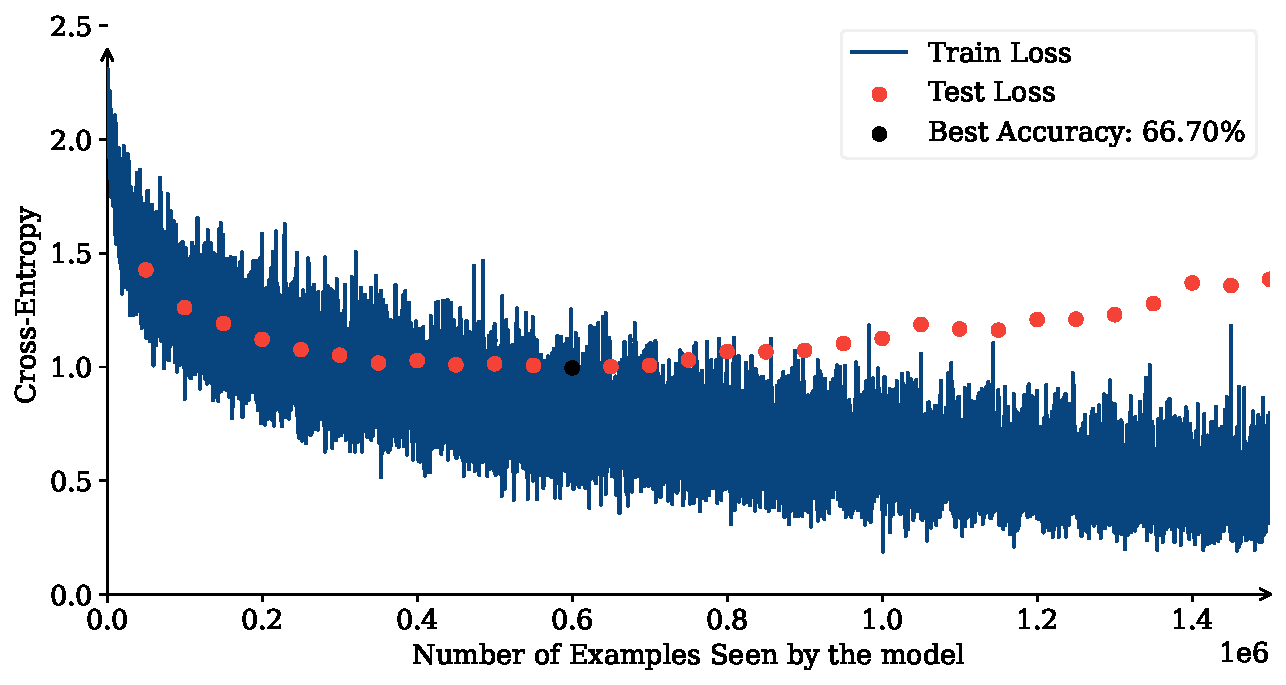
\includegraphics[width = 0.7 \textwidth]{figures/cifar_cnn.pdf}
	\end{figure}
\end{frame}



\begin{frame}{}{Model 3}

	The Net is composed 6 convolutional layers and 3 linear layers:
	\begin{itemize}
		\item Conv $3\times 32 \times 32 \mapsto 32 \times 32 \times 32$ + BatchNorm2d + ReLU
		\item Conv $32\times 32 \times 32 \mapsto 64 \times 32 \times 32$ + ReLU
		\item Max Pooling $ 64 \times 32 \times 32 \mapsto 64 \times 16 \times 16$
		\item Conv $64\times 16 \times 16 \mapsto 128 \times 16 \times 16$ + BatchNorm2d + ReLU
		\item Conv $128\times 16 \times 16 \mapsto 128 \times 16 \times 16$ + ReLU
		\item Max Pooling $ 128 \times 16 \times 16 \mapsto 128 \times 8 \times 8$
		\item Conv $128\times 8 \times 8 \mapsto 256 \times 8 \times 8$ + BatchNorm2d + ReLU
		\item Conv $256\times 8 \times 8 \mapsto 256 \times 8 \times 8$ + ReLU
		\item Max Pooling $ 256 \times 8 \times 8 \mapsto 256 \times 4 \times 4$ + DropOut $p=0.05$
		\item Linear $4096 \mapsto 1024$ + ReLU
		\item Linear $1024 \mapsto 512$ + ReLU + DropOut $p=0.05$
		\item Linear $512 \mapsto 10$ + SoftMax
	\end{itemize}
	We have added Batch Normalization to improve the training stability and Drop Out to reduce overfitting.
\end{frame}

\begin{frame}{}{Model 3 without Batch Normalization and Drop Out}
	\begin{figure}
		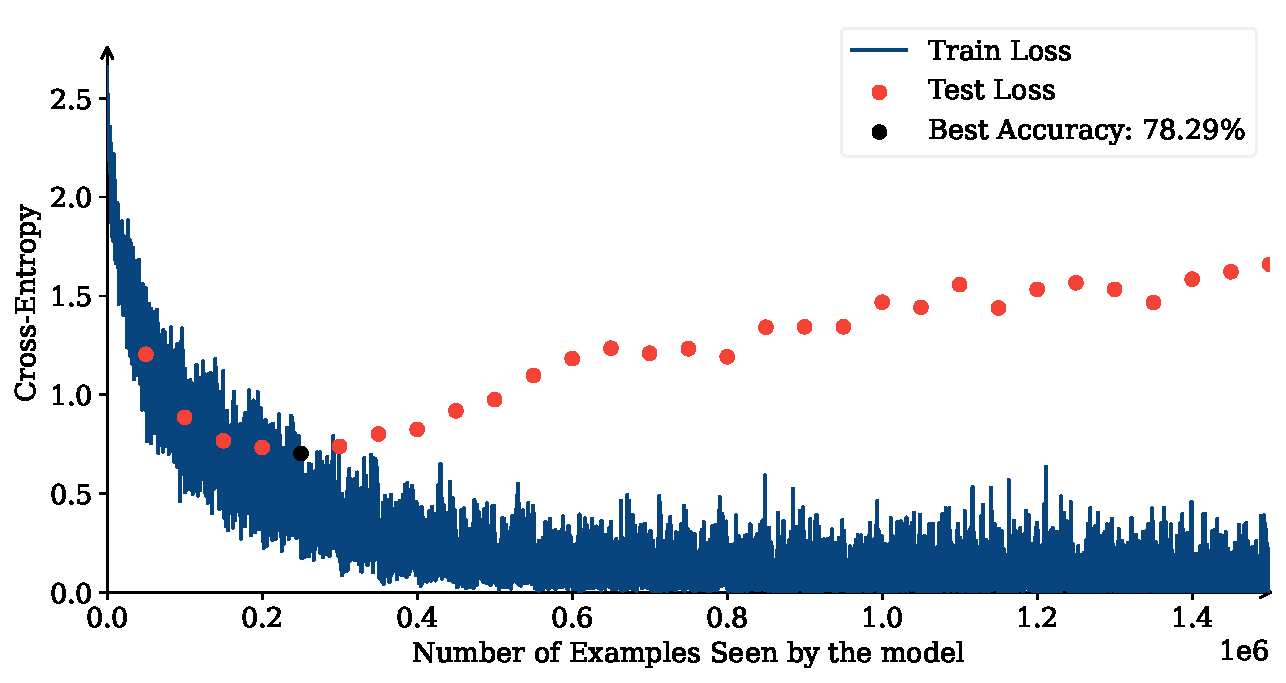
\includegraphics[width = 0.7 \textwidth]{figures/cifar_large_cnn.pdf}
	\end{figure}
\end{frame}

\begin{frame}{}{Batch Normalization}
	Batch normalization is used to normalize the activations of a layer within a batch of data.
	\begin{itemize}
		\item This helps to prevent the problem of vanishing or exploding gradients and also speeds up the training process.
		\item 	By normalizing the activations, batch normalization helps to stabilize the distribution of the inputs to each layer, reducing the covariate shift and allowing the network to learn more effectively.
	\end{itemize}


\end{frame}

\begin{frame}{}{Batch Normalization}
	\begin{small}
		\begin{algorithm}[H]
			\caption{Batch Normalization during training}
			\begin{algorithmic}[1]
				\FOR{each $x_i$ in a mini-batch $B$ of size $b$}
				\STATE Compute the mean $\mu_B$ and variance $\sigma_B^2$ of the features in the mini-batch $B$.
				$$\mu_B = \frac{1}{b}\sum_ix_i \quad \mbox{and} \quad\sigma_B^2=\frac{1}{m}\sum_i\left(x_i-\mu_B\right)^2 $$
				\STATE Normalize each feature $x_i$ in the mini-batch $B$ using $\mu_B$ and $\sigma_B^2$.
				$$\bar x_i = \frac{x_i-\mu_B}{\sqrt{\sigma_B^2 + \varepsilon}} $$
				\STATE Scale and shift each normalized feature $x_i$ using two learnable parameters $\gamma$ and $\beta$ respectively.
				$$ y_i = \gamma \bar x_i + \beta $$
				\STATE Update the moving average of the mean and variance for inference:
				$$
					\mu = (1-\gamma)\mu + \gamma \mu_B \quad \mbox{and} \quad \sigma^2 = (1-\gamma)\sigma^2 + \gamma \sigma_B^2 $$
				\ENDFOR
			\end{algorithmic}
		\end{algorithm}
	\end{small}
\end{frame}

\begin{frame}{}{Batch Normalization}
	At inference:
	\begin{algorithm}[H]
		\caption{Batch Normalization at inference}
		\begin{algorithmic}[1]
			\FOR{each $x_i$}
			\STATE Normalize each feature $x_i$ using the moving average of the mean and variance:
			$$\bar x_i = \frac{x_i-\mu}{\sqrt{\sigma^2 + \varepsilon}} $$
			\STATE Scale and shift each normalized feature $x_i$ using two learnable parameters $\gamma$ and $\beta$ respectively.
			$$ y_i = \gamma \bar x_i + \beta $$
			\ENDFOR
		\end{algorithmic}
	\end{algorithm}
\end{frame}

\begin{frame}{}{Model 3 without Drop Out}
	\begin{figure}
		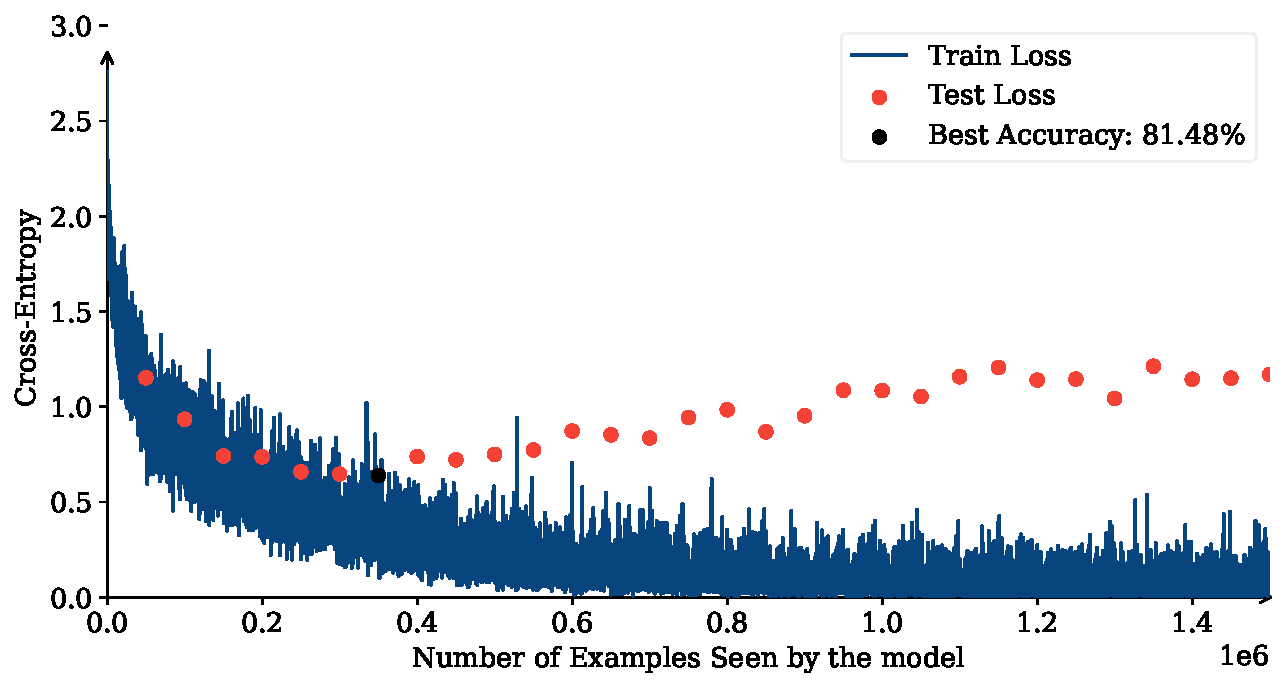
\includegraphics[width = 0.7 \textwidth]{figures/cifar_large_cnn_bn.pdf}
	\end{figure}
\end{frame}


\begin{frame}{}{Drop out}
	Dropout is a regularization technique in neural networks where \alert{during training}, a portion of the nodes are randomly "dropped out" or ignored during each iteration. This helps prevent over-fitting by preventing the model from relying too heavily on any one node. The result is a more robust and generalizable model that can better handle unseen data.
	\begin{figure}
		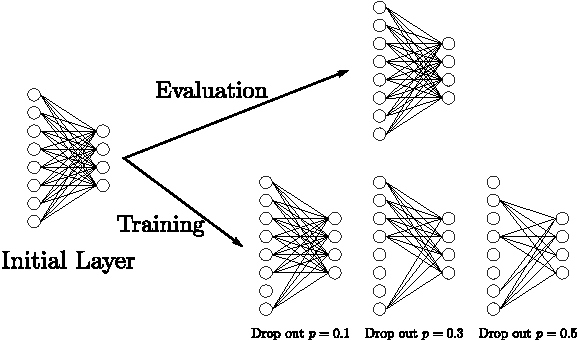
\includegraphics[width=0.7\textwidth]{figures/dropout.pdf}
	\end{figure}
\end{frame}

\begin{frame}{}{Model 3}
	\begin{figure}
		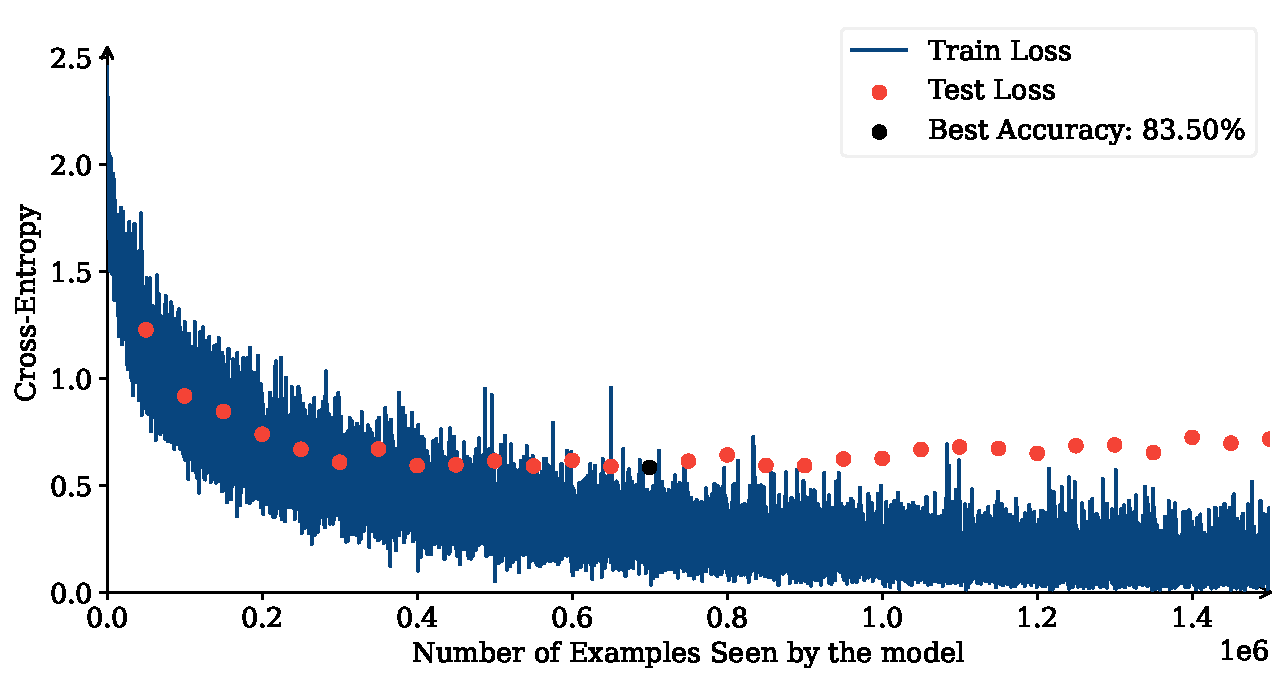
\includegraphics[width = 0.7 \textwidth]{figures/cifar_large_cnn_bn_dropout.pdf}
	\end{figure}
\end{frame}

\begin{frame}{}{Model 3}
	\begin{figure}
		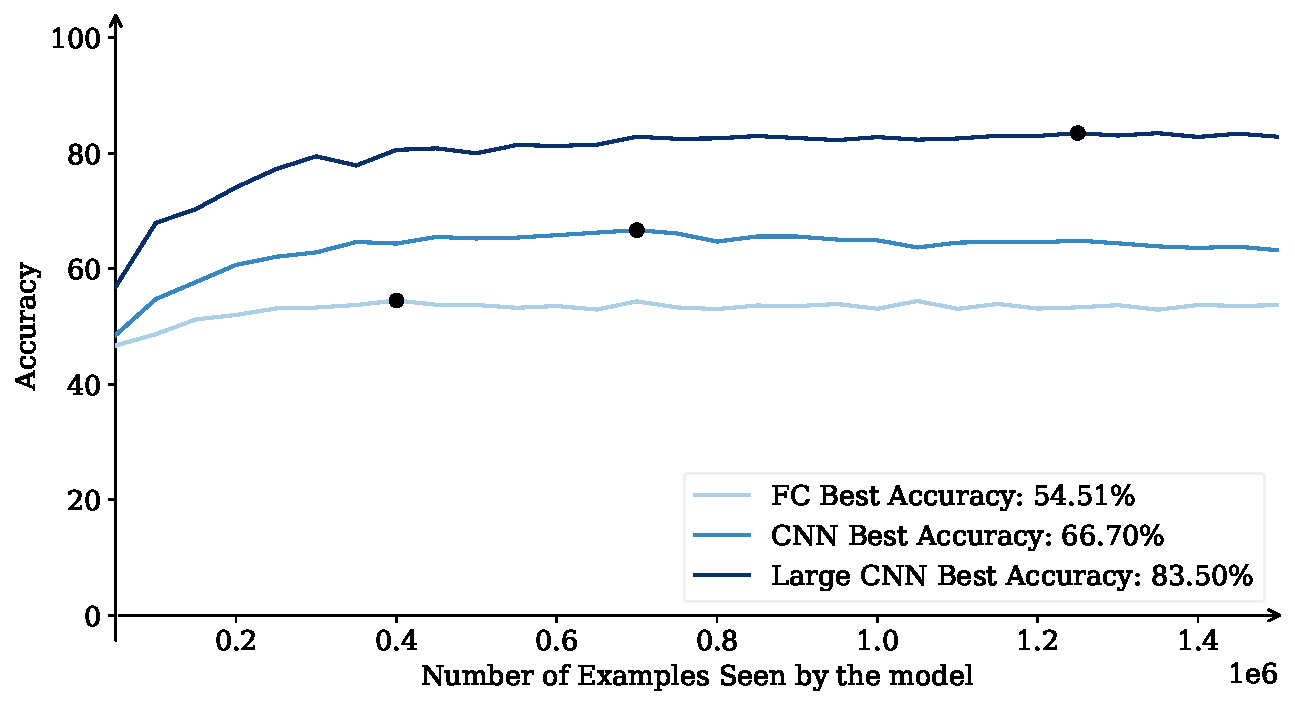
\includegraphics[width = 0.7 \textwidth]{figures/accuracies_cifar_cnn.pdf}
	\end{figure}
\end{frame}

\begin{frame}
	\begin{figure}
		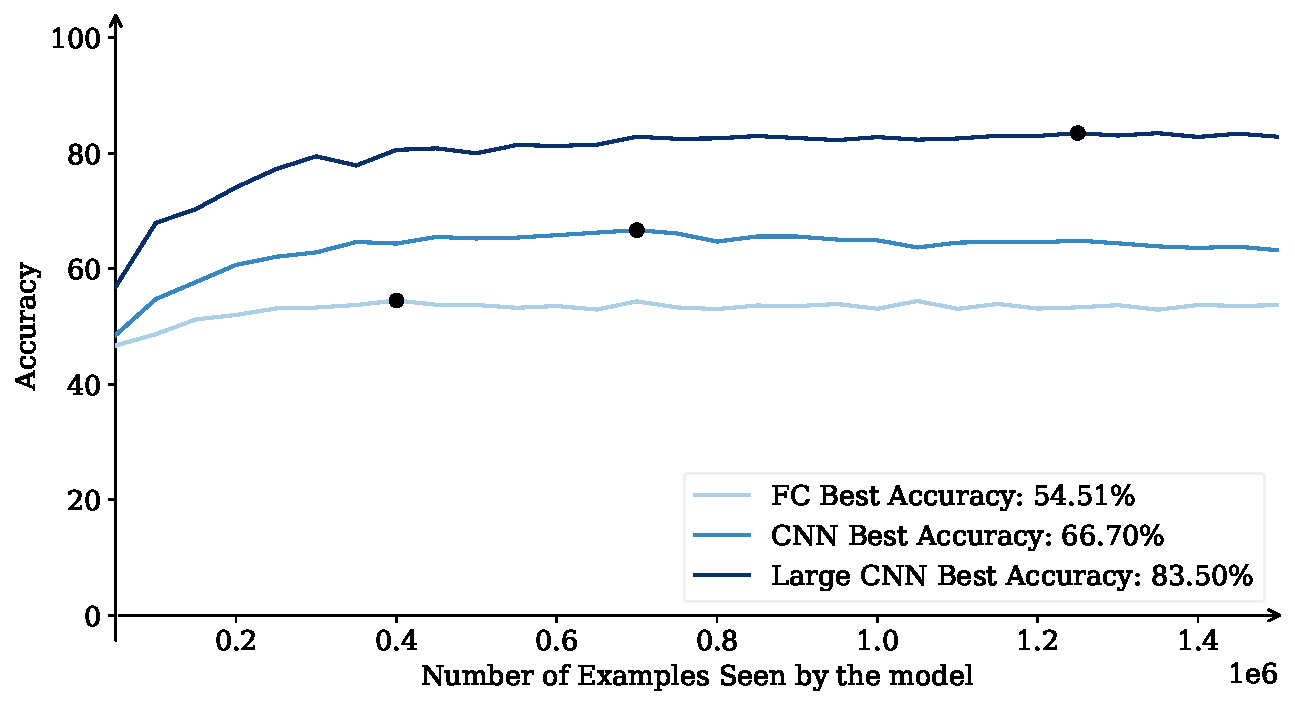
\includegraphics[width = 0.7 \textwidth]{figures/accuracies_cifar_fc_cnn.pdf}
	\end{figure}
\end{frame}

\begin{frame}{}{Intuition behind channels}
	To examine the information captured by different channels in a Neural Network, we can compare their output on a dataset. For a given input $x$, we can compute the similarity between the output of a specific channel and the same channel for other images in the dataset.
	\begin{figure}
		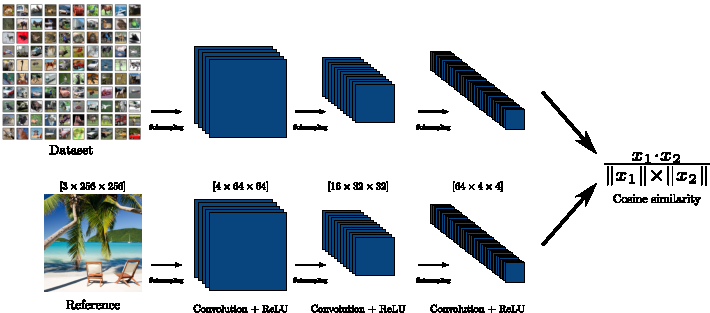
\includegraphics[width = 0.8 \textwidth]{figures/Cosine_channels.pdf}
	\end{figure}
\end{frame}
\begin{frame}{}{Intuition behind channels}
	\begin{figure}
		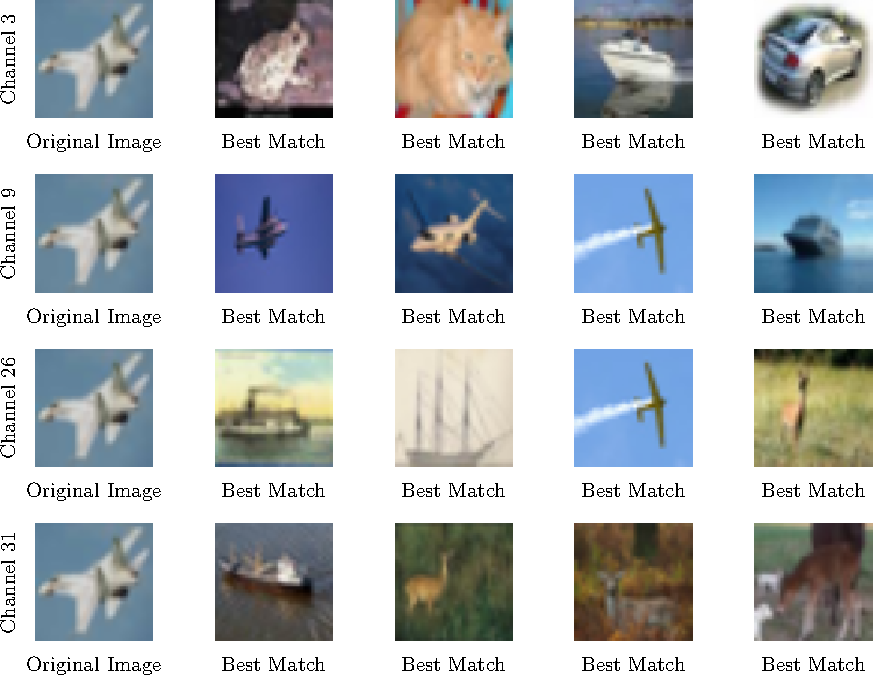
\includegraphics[width = 0.6 \textwidth]{figures/cifar10avion.pdf}
	\end{figure}
\end{frame}

\begin{frame}{}{Intuition behind channels}
	\begin{figure}
		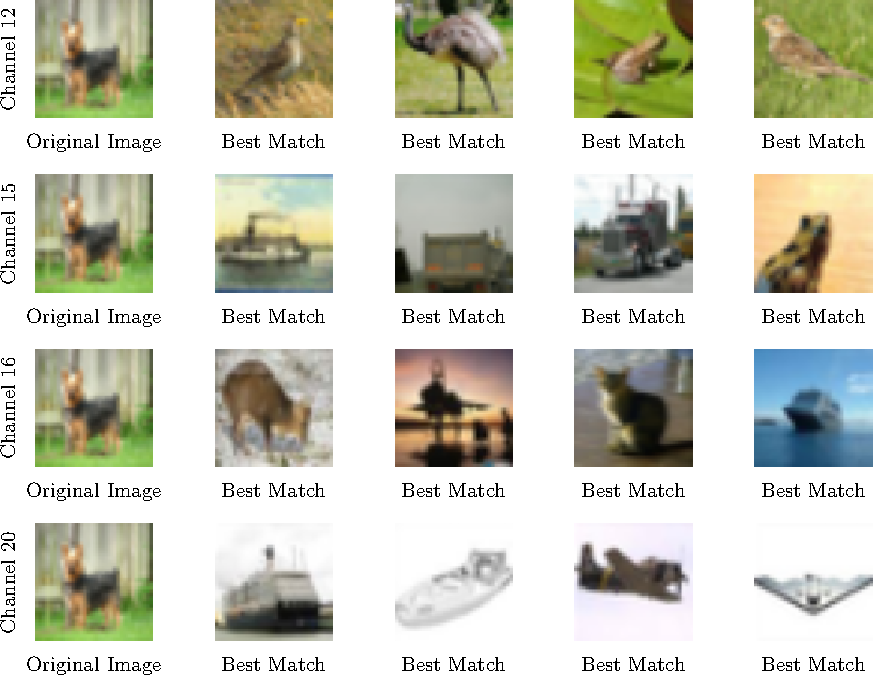
\includegraphics[width = 0.6 \textwidth]{figures/cifar10caniche.pdf}
	\end{figure}
\end{frame}
\begin{frame}{}{Intuition behind channels}
	\begin{figure}
		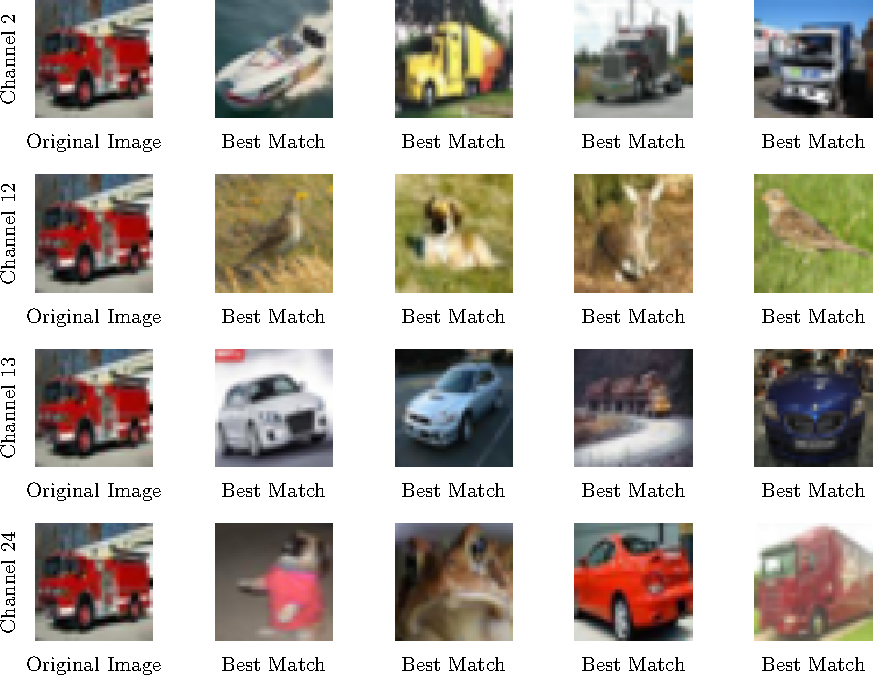
\includegraphics[width = 0.6 \textwidth]{figures/cifar10camion.pdf}
	\end{figure}
\end{frame}
\begin{frame}{}{Intuition behind channels}
	\begin{figure}
		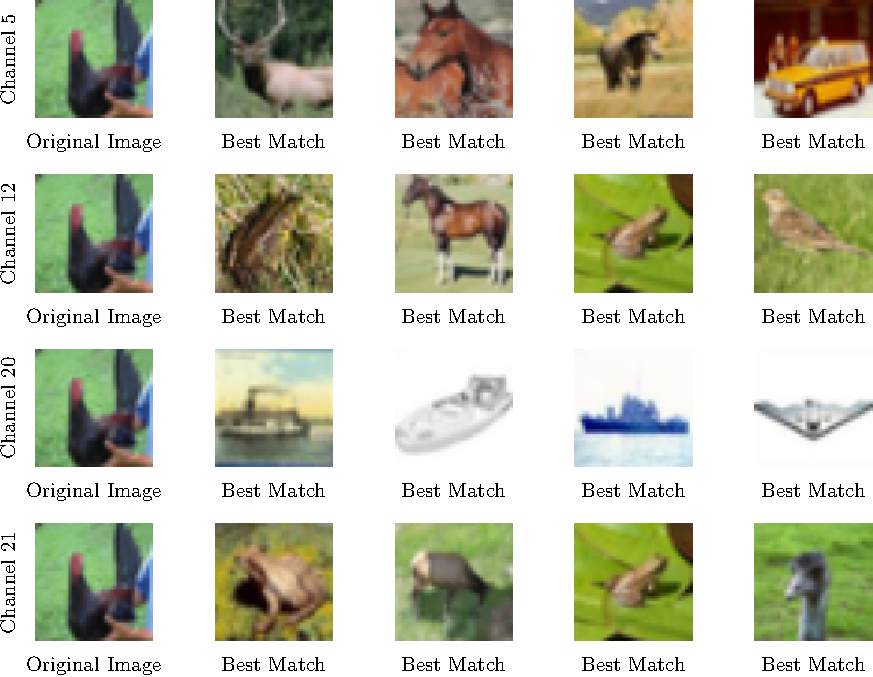
\includegraphics[width = 0.6 \textwidth]{figures/cifar10poulet.pdf}
	\end{figure}
\end{frame}


\begin{frame}{TP2: The Convolutional Neural Network}{Introduction to CNN and CIFAR-10 dataset}
	Link to the notebook (ipynb): \href{
		https://lamsade.dauphine.fr/~averine/EM_IASD/TP2.ipynb}{TP2.ipynb}\\
	Link to the notebook (html): \href{run:../notebook_pedagogiques/CNN.html}{CNN.html}
\end{frame}

\section{Recurrent Neural Networks}
\begin{frame}
	Recurrent Networks (RNNs) are a type of neural network that are specifically designed to handle sequential data, whereas CNNs are more suited for image and grid-like data. The main difference between RNNs and CNNs lies in the way they process data, with RNNs considering the sequence of elements and their interdependencies, while CNNs focus on capturing local patterns within the input.
\end{frame}

\subsection{Recurrent Block}

\begin{frame}
	A  Recurrent Network  is a type of neural network that contains a loop mechanism, allowing previous outputs to be used as inputs for future computations. This creates a form of memory that allows the network to process sequential data with variable-length sequences.
	\begin{figure}
		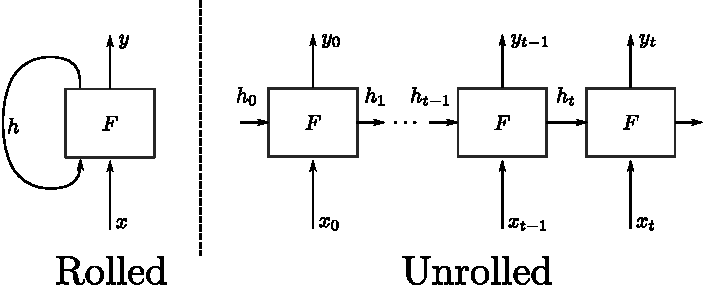
\includegraphics[width=0.7\textwidth]{figures/RNN.pdf}
	\end{figure}
\end{frame}
\begin{frame}
	\begin{columns}[c, onlytextwidth]
		\column{0.7\textwidth}
		Some of the limitations of Vanilla RNNs:
		\begin{itemize}
			\item Vanishing gradient problem: The gradient signals used to update the weights during training can become very small, making it difficult to train RNNs effectively.

			\item Exploding gradient problem: On the other hand, gradients can become too large and cause numeric instability, making it difficult to train RNNs effectively.

			\item Short-term memory: Vanilla RNNs have difficulty retaining information over long periods of time, making them unsuitable for tasks that require remembering information from previous time steps.

			\item Computational limitations: RNNs can be computationally intensive, making it difficult to apply them to large sequences of data.

			\item Difficulty with parallelization: The sequential nature of RNNs can make it difficult to take advantage of parallel processing to speed up training and inference.
		\end{itemize}
		\column{0.3\textwidth}
		\begin{figure}
			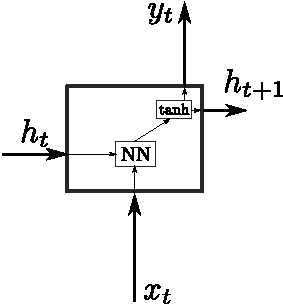
\includegraphics[width=0.8\textwidth]{figures/RNN_NN.pdf}
		\end{figure}
	\end{columns}
\end{frame}

\subsection{LSTM  and GRU}
\begin{frame}{}{LSTM}
	Long Short-Term Memory (LSTM) networks are a variant of recurrent neural networks (RNNs) that overcome some of the limitations of traditional RNNs, such as the vanishing gradient problem and difficulty in learning long-term dependencies. LSTM networks introduce memory cells, gates, and a process for updating cells, which allows them to selectively preserve information from previous time steps.

	\begin{figure}
		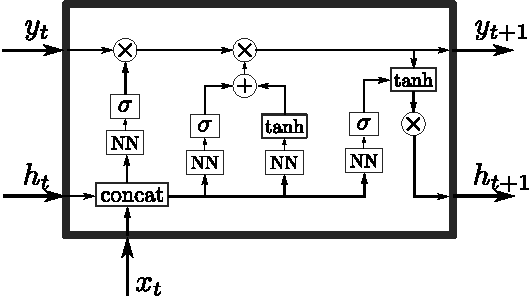
\includegraphics[width=0.7\textwidth]{figures/LSTM.pdf}
	\end{figure}
\end{frame}

\begin{frame}{}{LSTM}
	Long Short-Term Memory (LSTM) networks are a variant of recurrent neural networks (RNNs) that overcome some of the limitations of traditional RNNs, such as the problem of vanishing gradients and the difficulty of learning long-term dependencies. LSTM networks introduce memory cells, gates, and a process for updating cells, which allows them to selectively preserve information from previous time steps.

	\begin{figure}
		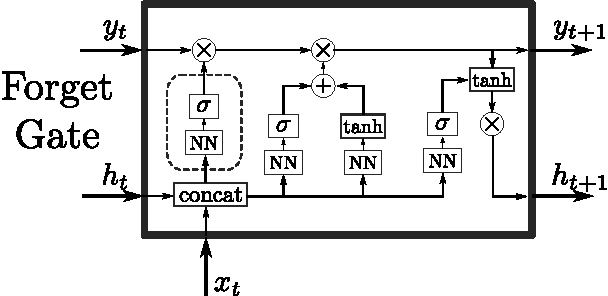
\includegraphics[width=0.6\textwidth]{figures/LSTM_forget.pdf}
	\end{figure}
\end{frame}
\begin{frame}{}{LSTM}
	Long Short-Term Memory (LSTM) networks are a variant of recurrent neural networks (RNNs) that overcome some of the limitations of traditional RNNs, such as the vanishing gradient problem and difficulty in learning long-term dependencies. LSTM networks introduce memory cells, gates, and a process for updating the cells, which allows them to selectively preserve information from previous time steps.

	\begin{figure}
		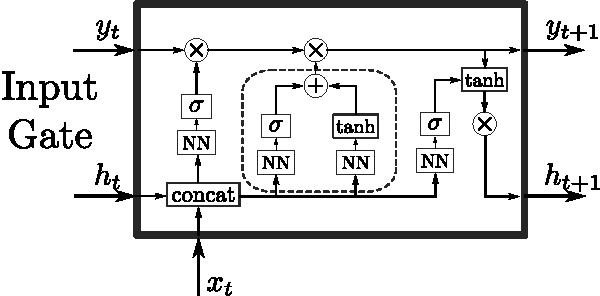
\includegraphics[width=0.6\textwidth]{figures/LSTM_input.pdf}
	\end{figure}
\end{frame}
\begin{frame}{}{LSTM}
	Long Short-Term Memory (LSTM) networks are a variant of recurrent neural networks (RNNs) that overcome some of the limitations of traditional RNNs, such as the vanishing gradient problem and difficulty in learning long-term dependencies. LSTM networks introduce memory cells, gates, and a process for updating the cells, which allows them to selectively preserve information from previous time steps.

	\begin{figure}
		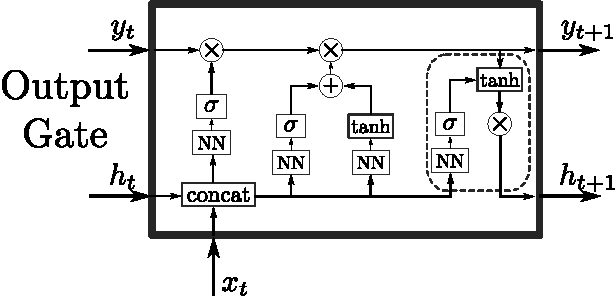
\includegraphics[width=0.6\textwidth]{figures/LSTM_output.pdf}
	\end{figure}
\end{frame}

\begin{frame}{}{Limits of LSTM}
	Limitations of LSTM RNNs:
	\begin{itemize}
		\item High computational cost: LSTMs are computationally more expensive compared to other traditional neural network models due to the presence of multiple gates and their sequential processing nature.

		\item Vanishing Gradient Problem: LSTMs, like any other RNNs, are prone to the vanishing gradient problem when the sequences are too long, making it difficult for the model to learn long-term dependencies.

		\item Overfitting: LSTMs are complex models and are more susceptible to overfitting compared to simple feedforward networks.

		\item Difficult to parallelize: Due to the sequential nature of LSTMs, they are difficult to parallelize and can take longer to train.

		\item Gradient Explosion: LSTMs can also suffer from the gradient explosion problem, where the gradients can become too large and cause numerical instability during training.
	\end{itemize}
\end{frame}

\begin{frame}{}{GRU}
	GRU blocks, or Gated Recurrent Units, are a type of recurrent neural network architecture that are similar to LSTMs in their function and ability to process sequential data. GRUs were introduced as a simplification of LSTMs, with the aim of reducing the number of parameters in the network and improving computational efficiency. GRUs achieve this by merging the forget and input gates in LSTMs into a single update gate, effectively combining the two operations in a single step.
	\begin{figure}
		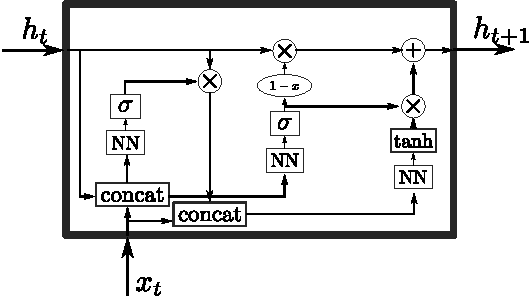
\includegraphics[width=0.6\textwidth]{figures/GRU.pdf}
	\end{figure}
\end{frame}



\begin{frame}{}{GRU}
	GRU blocks, or Gated Recurrent Units, are a type of recurrent neural network architecture that are similar to LSTMs in their function and ability to process sequential data. GRUs were introduced as a simplification of LSTMs, with the aim of reducing the number of parameters in the network and improving computational efficiency. GRUs achieve this by merging the forget and input gates in LSTMs into a single update gate, effectively combining the two operations in a single step.
	\vfill
	\begin{figure}
		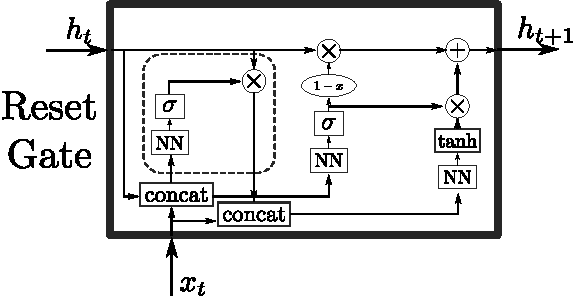
\includegraphics[width=0.6\textwidth]{figures/GRU_reset.pdf}
	\end{figure}
\end{frame}

\begin{frame}{}{GRU}
	GRU blocks, or Gated Recurrent Units, are a type of recurrent neural network architecture that are similar to LSTMs in their function and ability to process sequential data. GRUs were introduced as a simplification of LSTMs, with the aim of reducing the number of parameters in the network and improving computational efficiency. GRUs achieve this by merging the forget and input gates in LSTMs into a single update gate, effectively combining the two operations in a single step.
	\vfill
	\begin{figure}
		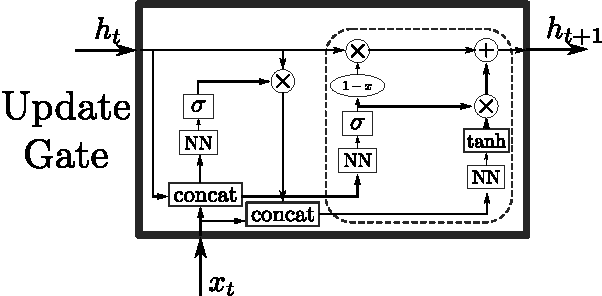
\includegraphics[width=0.6\textwidth]{figures/GRU_update.pdf}
	\end{figure}
\end{frame}

\begin{frame}

	Limitations of GRU RNNs:
	\begin{itemize}
		\item 	Computational complexity: GRUs are more computationally efficient than LSTMs but still more complex than feedforward neural networks.

		\item Long-term dependencies: GRUs may struggle with capturing long-term dependencies in sequences, although they perform better in this regard than vanilla RNNs.


		\item Vanishing gradient problem: GRUs can still be affected by the vanishing gradient problem that plagues all RNN models. This problem makes it difficult for the model to learn from long sequences.

		\item Non-stationary data: GRUs may struggle with nonstationary data, where the statistical properties of the data change over time.
	\end{itemize}
\end{frame}
\begin{frame}{}{Application of RNNs}
	Applications of RNNs:
	\begin{itemize}
		\item Natural language processing (NLP): Using RNNs for text classification, language translation, and text generation.
		\item Time-series prediction: Using RNNs to make predictions based on sequential data, such as stock prices and weather patterns.
		\item Speech recognition: Using RNNs for speech-to-text conversion.
	\end{itemize}
\end{frame}



\section{Transformer and Attention Mechanism}
\begin{frame}
	Transformers and Attention Mechanisms are recent advancements in deep learning, widely used for sequential data processing, especially in NLP. Unlike RNNs, which apply the same weights iteratively, Transformers leverage self-attention to dynamically assign importance to different sequence elements. This enhances their ability to capture long-range dependencies, improving NLP performance.
\end{frame}
\subsection{Self-Attention Mechanism}
\begin{frame}
	The self-attention mechanism in Transformers computes the importance of each token relative to others in a sequence. It generates a weighted representation where the most relevant tokens contribute more. Mathematically, self-attention is computed as:

	\[
		\mathrm{Attention}(Q, K, V) = \mathrm{Softmax}\left(\frac{QK^T}{\sqrt{d_k}} \right)V
	\]

	where \( Q \in \mathbb{R}^{m\times d_k} \), \( K \in \mathbb{R}^{n\times d_k} \), and \( V \in \mathbb{R}^{n\times d_v} \) are the query, key, and value matrices derived from the input sequence. The softmax function ensures proper weighting, producing the final representation.

\end{frame}
\begin{frame}
	\begin{columns}[c, onlytextwidth]
		\column{0.6 \textwidth}
		\textbf{Intuition behind the self-attention mechanism:}
		\begin{itemize}
			\item The \textbf{query} and \textbf{key} matrices measure the similarity between different tokens in the sequence.
			\item These similarity scores determine how much each \textbf{value} contributes to the final output.
			\item The resulting \textbf{weighted sum} of the values represents the output of the self-attention mechanism.
			\item This process captures the relationships between different parts of the input sequence, allowing the model to focus on the most relevant elements.
		\end{itemize}
		\column{0.4 \textwidth}
		\begin{figure}
			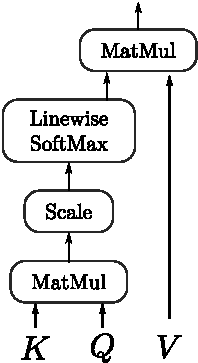
\includegraphics[width=0.6\textwidth]{figures/AttentionMech.pdf}
		\end{figure}
	\end{columns}
\end{frame}
\begin{frame}
	Illustration (source: \href{https://learnopencv.com/attention-mechanism-in-transformer-neural-networks/}{Understanding Attention Mechanism in Transformer Neural Networks}):
	\begin{figure}
		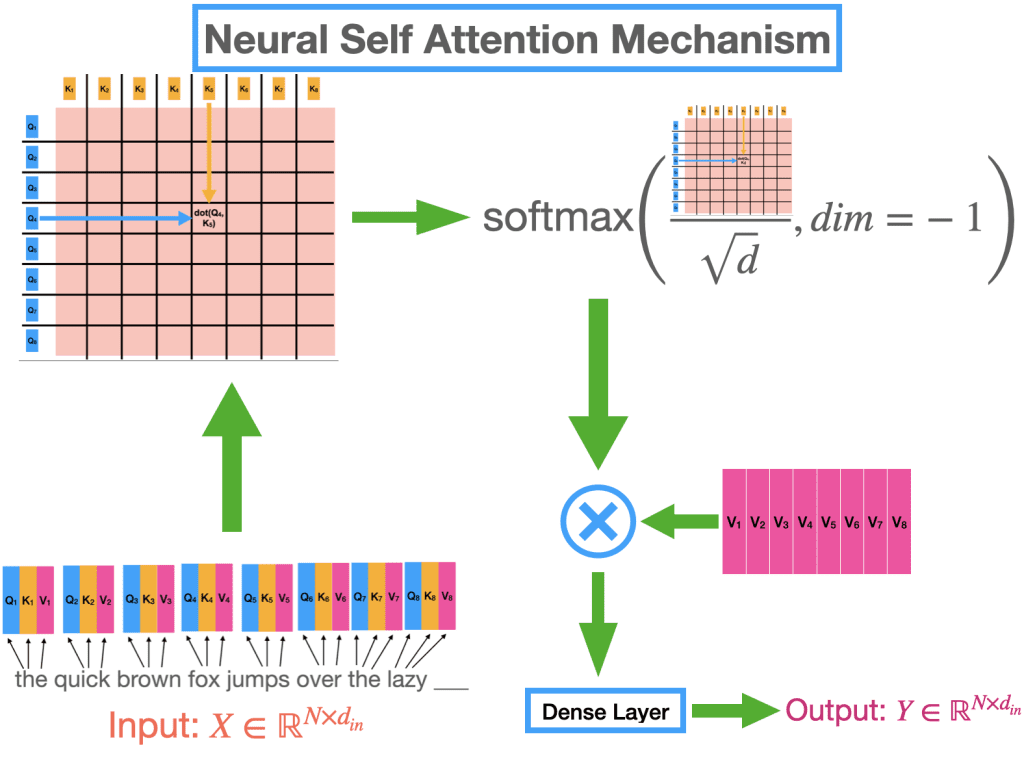
\includegraphics[width=0.5\textwidth]{figures/neural-self-attention-cover-picture-1024x767.png}
	\end{figure}
\end{frame}


\begin{frame}{}{Multi-Head Attention}
	\begin{columns}[c, onlytextwidth]
		\column{0.6 \textwidth}
		In Multi-head Attention, the self-attention mechanism is performed multiple times in parallel with different weight matrices, before being concatenated and once again projected, leading to a more robust representation of the input sequence. The intuition behind the three matrices ($Q$, $K$, $V$) remains the same as in self-attention, with $Q$ representing the query, $K$ the key and $V$ the value. Each head performs an attention mechanism on the input sequence, capturing different aspects and dependencies of the data, before being combined to form a more comprehensive representation of the input.
		\column{0.4 \textwidth}
		\begin{figure}
			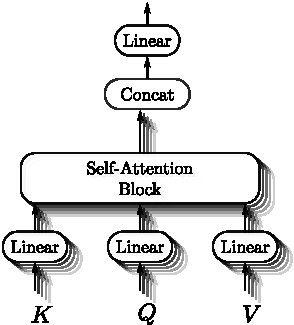
\includegraphics[width=0.8\textwidth]{figures/AttentionMechMulti.pdf}
		\end{figure}
	\end{columns}
\end{frame}

\begin{frame}{}{Visualizing Multi-Head Attention}
	\begin{columns}[c, onlytextwidth]
		\column{0.35 \textwidth}

		Visualizing Self-Attention for Image: \\
		\href{https://epfml.github.io/attention-cnn/}{Link}

		\column{0.65 \textwidth}
		\begin{figure}
			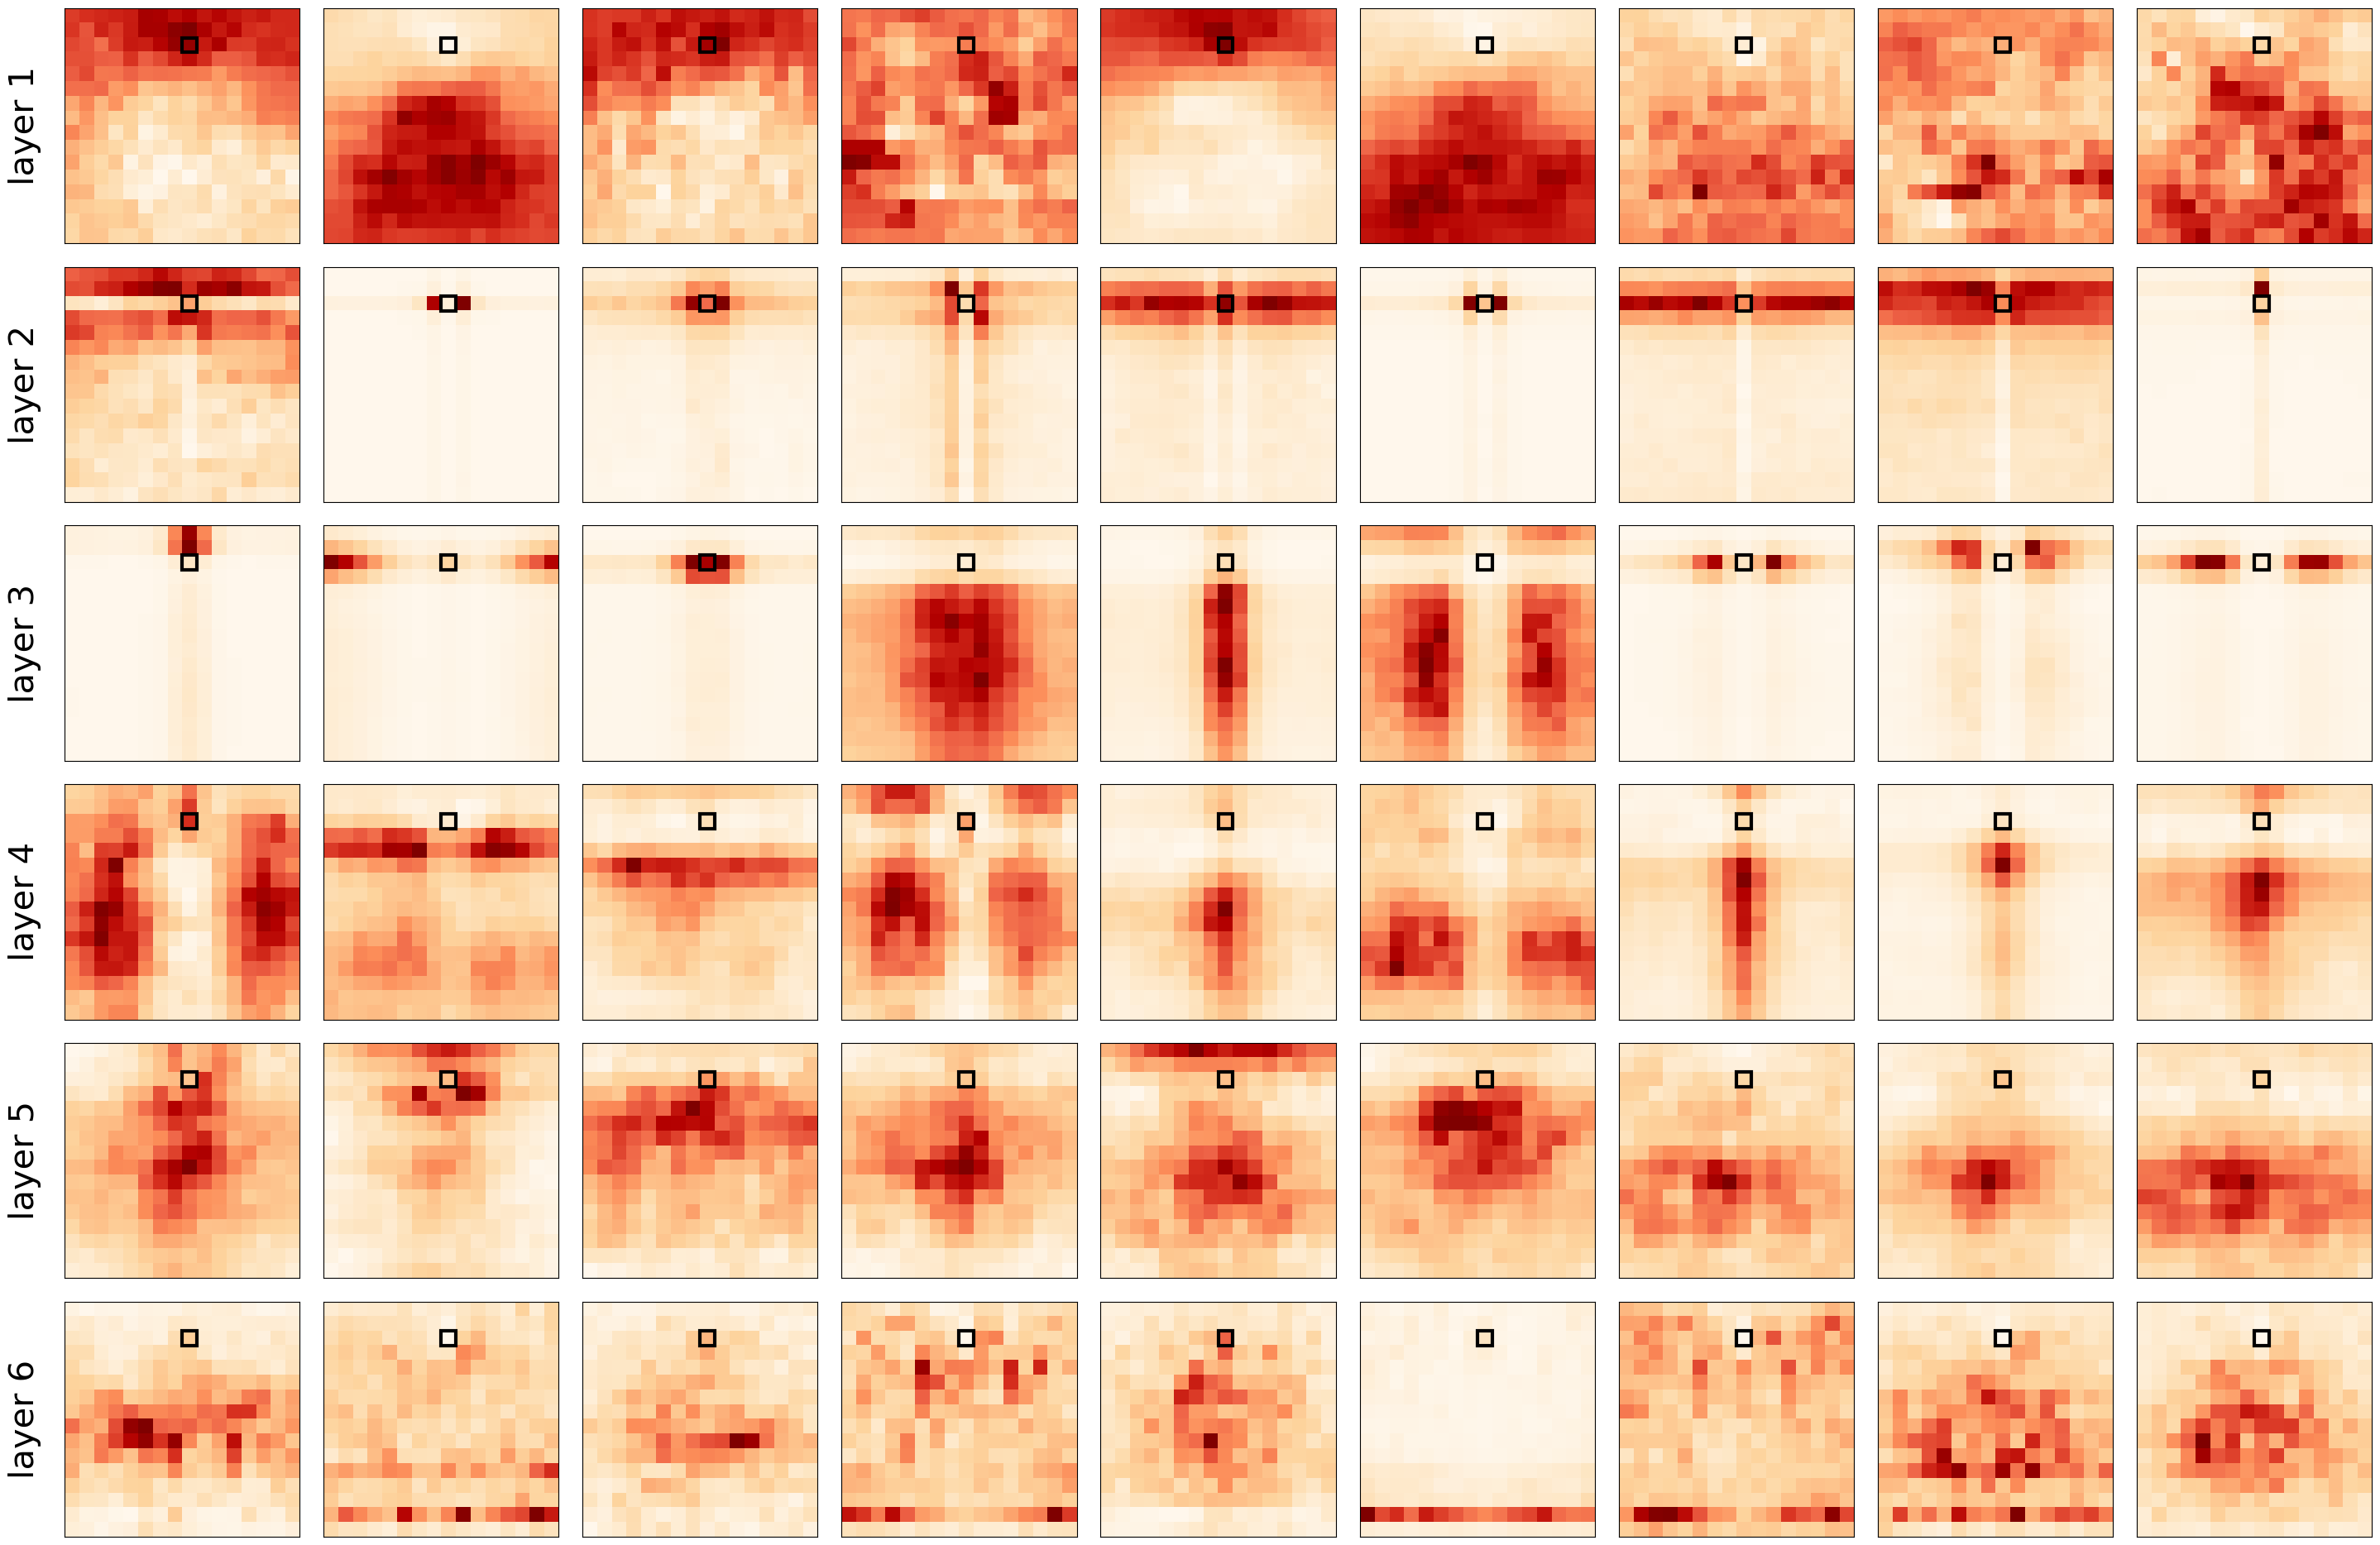
\includegraphics[width=0.8\textwidth]{figures/img_2_8.png}
		\end{figure}
	\end{columns}
\end{frame}

\subsection{Transformers Model}


\begin{frame}
	\begin{columns}[t, onlytextwidth]
		\column{0.6 \textwidth}

		Transformers are neural network models that use an encoder-decoder architecture. The encoder takes the input sequence and converts it into a continuous hidden representation, which is then passed to the decoder to generate the output sequence. The architecture of the transformer model is designed to allow the model to process the entire sequence in parallel, rather than processing one element at a time like in traditional RNNs.\newline

		Training of transformers involves optimizing a loss function that measures the difference between the model predictions and the true outputs. This loss function is usually based on the cross entropy between the predicted and true sequences.\newline

		The encoder-decoder mechanism is commonly referred to as the seq2seq mechanism.
		\column{0.05 \textwidth}
		\column{0.4 \textwidth}
		\begin{figure}
			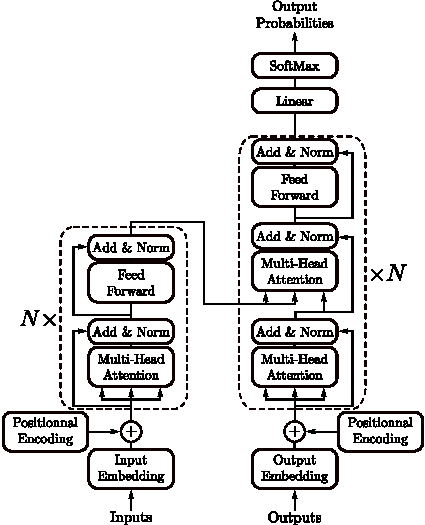
\includegraphics[width=0.9\textwidth]{figures/transformers.pdf}
		\end{figure}
	\end{columns}

\end{frame}



\makepart{Techniques to Improve Deep Learning Training}
\section{Techniques to Improve Deep Learning Training}
\begin{frame}
    \frametitle{Techniques to Improve Deep Learning Training}
    \begin{itemize}
        \item \textbf{Batch Normalization} - Seen
        \item \textbf{Dropout} - Seen
        \item \textbf{Data Augmentation}
        \item \textbf{Learning Rate Scheduling}
        \item \textbf{Early Stopping}
        \item \textbf{Gradient Clipping}
        \item \textbf{Weight Initialization}
        \item \textbf{Regularization}
        \item \textbf{GPU Acceleration}
    \end{itemize}
\end{frame}
\subsection{Data Augmentation}
\begin{frame}{}{Data Augmentation}
    \begin{itemize}
        \item Data Augmentation is a technique to increase the diversity of your training set by applying random (but realistic) transformations to the training images.
        \item The goal is to train a model that is robust to these transformations.
        \item For example, you can randomly rotate, scale, and flip the images in your training set.
        \item This helps expose the model to different aspects of the data and reduce overfitting.
    \end{itemize}
    \begin{figure}
        \centering
        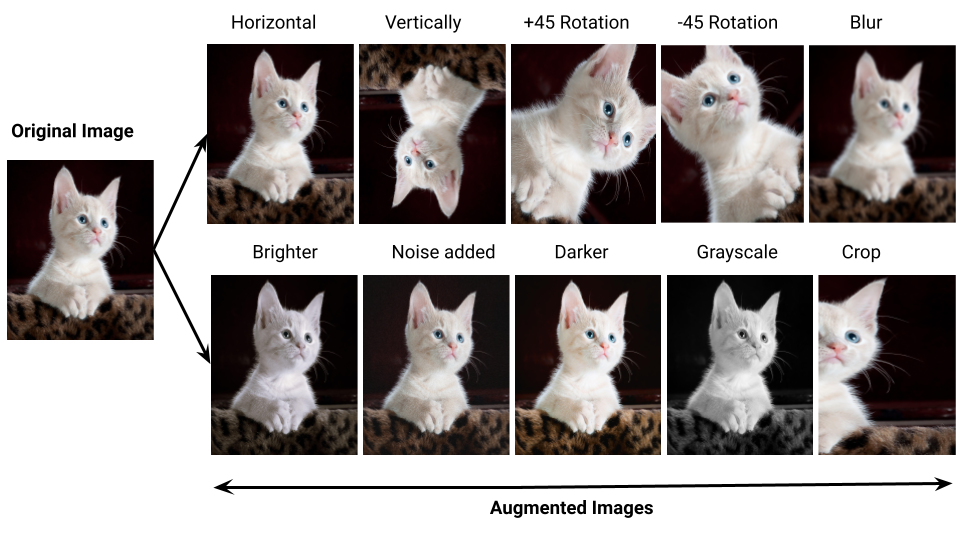
\includegraphics[width=0.6\textwidth]{figures/dataaug.png}
    \end{figure}
\end{frame}

\subsection{Learning Rate Scheduling}
\begin{frame}{}{Learning Rate Scheduling}
    \begin{itemize}
        \item The learning rate is one of the most important hyperparameters to tune for your deep learning model. The learning rate determines how quickly the model learns the optimal weights and how refined the gradient descent process is.
        \item If the learning rate is too high, the model may not converge or converge to a higher loss. If it is too low, the model may take too long to train.

              \only<2>{\item Learning rate scheduling is a technique to adjust the learning rate during training. For example, you can start with a high learning rate and then decrease it over time.}
    \end{itemize}
    \begin{center}
        \begin{tikzpicture}
            \begin{axis}[
                    width=15cm, height=5cm,
                    xlabel={Epochs},
                    ylabel={Loss},
                    ymin=0, ymax=2,
                    xmin=0, xmax=50,
                    legend style={at={(0.97,0.97)},anchor=north east},
                    grid=major,
                    grid style={dashed, gray!30},
                ]

                % Slow reducing loss (low learning rate, lower final loss)
                \addplot [
                    thick,
                    smooth,
                    primary,
                ] coordinates {
                        (0, 1.8)
                        (5, 1.4)
                        (10, 1.0)
                        (15, 0.6)
                        (20, 0.35)
                        (25, 0.25)
                        (30, 0.2)
                        (35, 0.15)
                        (40, 0.1)
                        (45, 0.08)
                        (50, 0.08)
                    };
                \addlegendentry{Low learning rate}

                % Fast reducing loss (high learning rate, higher final loss)
                \addplot [
                    thick,
                    smooth,
                    secondary,
                    dashed,
                ] coordinates {
                        (0, 1.8)
                        (5, 0.9)
                        (10, 0.5)
                        (15, 0.4)
                        (20, 0.35)
                        (25, 0.34)
                        (30, 0.34)
                        (35, 0.34)
                        (40, 0.34)
                        (45, 0.34)
                        (50, 0.34)
                    };
                \addlegendentry{High learning rate}
                \only<2>{
                    \addplot [
                        thick,
                        smooth,
                        tertiary,
                    ] coordinates {
                            (0, 1.8)
                            (5, 0.9)
                            (10, 0.5)
                            (15, 0.4)
                            (20, 0.35)
                            (25, 0.34)
                            (30, 0.34)
                            (32, 0.34)
                            (35, 0.12)
                            (40, 0.1)
                            (45, 0.08)
                            (50, 0.08)
                        };
                    \addlegendentry{Learning rate scheduled} }
            \end{axis}
        \end{tikzpicture}
    \end{center}
\end{frame}

\subsection{Early Stopping}
\begin{frame}{}{Early Stopping}
    \begin{itemize}
        \item Early stopping is a technique to prevent overfitting by stopping the training process when the model's performance on the validation set starts to degrade.
        \item The idea is to monitor the validation loss during training and stop training when the validation loss stops decreasing.
    \end{itemize}
    \vspace{2cm}
    \begin{center}
        \begin{tikzpicture}
            \begin{axis}[
                    width=15cm, height=5cm,
                    xlabel={Epochs},
                    ylabel={Loss},
                    ymin=0, ymax=2,
                    xmin=0, xmax=50,
                    legend style={at={(0.97,0.97)},anchor=north east},
                    grid=major,
                    grid style={dashed, gray!30},
                ]

                % Training loss curve
                \addplot [
                    thick,
                    smooth,
                    primary,
                ] coordinates {
                        (0, 1.8)
                        (5, 1.3)
                        (10, 1.0)
                        (15, 0.7)
                        (20, 0.5)
                        (25, 0.4)
                        (30, 0.3)
                        (35, 0.25)
                        (40, 0.2)
                        (45, 0.15)
                        (50, 0.1)
                    };
                \addlegendentry{Training Loss}

                % Evaluation loss curve
                \addplot [
                    thick,
                    smooth,
                    secondary,
                    dashed,
                ] coordinates {
                        (0, 1.8)
                        (5, 1.4)
                        (10, 1.0)
                        (15, 0.8)
                        (20, 0.6)
                        (25, 0.5)
                        (30, 0.55)
                        (35, 0.6)
                        (40, 0.7)
                        (45, 0.85)
                        (50, 1.0)
                    };
                \addlegendentry{Evaluation Loss}

                % Early stopping marker
                \node at (axis cs: 25,0.5) [pin=above:{Early Stopping Point}] {};

            \end{axis}
        \end{tikzpicture}
    \end{center}
\end{frame}

\subsection{Gradient Clipping}
\begin{frame}{}{Gradient Clipping}
    \begin{itemize}
        \item Gradient clipping is a technique to prevent exploding gradients during training.
        \item Exploding gradients occur when the gradients of the loss function with respect to the model's parameters are too large.
        \item This can cause the model to diverge and fail to learn.
        \item Gradient clipping involves scaling the gradients if their norm exceeds a certain threshold.
    \end{itemize}
    \begin{center}
        \begin{tikzpicture}
            \begin{axis}[
                    width=15cm, height=5cm,
                    xlabel={Epochs},
                    ylabel={Loss},
                    ymin=0, ymax=3,
                    xmin=0, xmax=50,
                    legend style={at={(0.97,0.97)},anchor=north east},
                    grid=major,
                    grid style={dashed, gray!30},
                ]

                % Loss without gradient clipping (with sudden spikes)
                \addplot [
                    thick,
                    smooth,
                    primary,
                    dashed,
                ] coordinates {
                        (0, 2.5)
                        (5, 1.8)
                        (10, 1.3)
                        (15, 0.9)
                        (20, 0.6)
                        (25, 0.5)
                        (28, 1.7)
                        (35, 1.5)
                        (40, 1.3)
                        (45, 1.2)
                        (50, 1.15)
                    };
                \addlegendentry{Without Gradient Clipping}

                % Loss with gradient clipping
                \addplot [
                    thick,
                    smooth,
                    secondary,
                ] coordinates {
                        (0, 2.5)
                        (5, 1.8)
                        (10, 1.3)
                        (15, 0.9)
                        (20, 0.6)
                        (25, 0.4)
                        (30, 0.35)
                        (35, 0.3)
                        (40, 0.25)
                        (45, 0.2)
                        (50, 0.1)
                    };
                \addlegendentry{With Gradient Clipping}

            \end{axis}
        \end{tikzpicture}
    \end{center}
\end{frame}

\subsection{Optimizer Choice}
\begin{frame}{}{Optimizer Choice}
    \begin{itemize}
        \item The choice of optimizer can have a significant impact on the training process and the final performance of the model.
        \item Common optimizers include Stochastic Gradient Descent (SGD), Adam, RMSprop, and Adagrad.
        \item Each optimizer has its own strengths and weaknesses, and the choice of optimizer may depend on the specific problem and dataset.
    \end{itemize}
\end{frame}

\begin{frame}{}{Recall on SGD}
    \begin{itemize}
        \item Stochastic Gradient Descent (SGD) is a variant of gradient descent that updates the model weights using only a small batch of data at each iteration.
        \item The gradient is computed on a mini-batch of data {$(x_i, y_i)$} of size $m$:
              \[
                  g = \frac{1}{m} \sum_{i=1}^{m} \nabla_w L(f(x_i; w), y_i)
              \]
        \item The weights are then updated using the computed gradient:
              \[
                  w = w - \eta g
              \]
              where $\eta$ is the learning rate.
    \end{itemize}
\end{frame}

\begin{frame}{}{RMSprop}
    \begin{itemize}
        \item RMSprop is an adaptive learning rate optimization algorithm that adjusts the learning rate for each parameter based on the magnitude of the gradients.
        \item It maintains a moving average of the squared gradients:
              \[
                  E[g^2]_t = \beta E[g^2]_{t-1} + (1 - \beta) g_t^2
              \]
        \item The weights are then updated using the computed gradient and the moving average:
              \[
                  w = w - \frac{\eta}{\sqrt{E[g^2]_t + \epsilon}} g_t
              \]
              where $\epsilon$ is a small constant to prevent division by zero.
    \end{itemize}
\end{frame}

\begin{frame}{}{Adam}
    \begin{itemize}
        \item Adam (Adaptive Moment Estimation) is an optimization algorithm that combines the benefits of both RMSprop and momentum.
        \item It maintains a moving average of the gradients and the squared gradients:
              \[
                  m_t = \beta_1 m_{t-1} + (1 - \beta_1) g_t
              \]
              \[
                  v_t = \beta_2 v_{t-1} + (1 - \beta_2) g_t^2
              \]
        \item The weights are then updated using the computed gradient and the moving averages:
              \[
                  w = w - \frac{\eta}{\sqrt{v_t} + \epsilon} m_t
              \]
              where $\epsilon$ is a small constant to prevent division by zero.
    \end{itemize}
\end{frame}

\begin{frame}{}{Adagrad}
    \begin{itemize}
        \item Adagrad is an adaptive learning rate optimization algorithm that adjusts the learning rate for each parameter based on the magnitude of the gradients.
        \item It maintains a sum of the squared gradients:
              \[
                  G_t = G_{t-1} + g_t^2
              \]
        \item The weights are then updated using the computed gradient and the sum of squared gradients:
              \[
                  w = w - \frac{\eta}{\sqrt{G_t + \epsilon}} g_t
              \]
              where $\epsilon$ is a small constant to prevent division by zero.
    \end{itemize}
\end{frame}

\begin{frame}{}{Optimizer Comparison}
    \begin{columns}
        \begin{column}{0.4\textwidth}
            \begin{itemize}
                \item SGD is simple and effective, but may require careful tuning of the learning rate and momentum.
                \item RMSprop is effective for non-stationary objectives and works well in practice.
                \item Adam is widely used and often performs well across a variety of tasks, but may not always converge to the optimal solution.
                \item Adagrad is effective for sparse data, but may lead to a rapid decrease in the learning rate.
            \end{itemize}
        \end{column}
        \begin{column}{0.6\textwidth}
            \begin{figure}
                \animategraphics[autoplay,loop,width=0.4\textwidth]{15}{figures/sgd/sgd_}{0}{99}
            \end{figure}
        \end{column}
    \end{columns}
\end{frame}







\subsection{Weight Initialization}
\begin{frame}{}{Weight Initialization}
    \begin{itemize}
        \item Weight initialization is a technique to set the initial values of the weights in the model.
        \item The initial values of the weights can have a significant impact on the training process and the final performance of the model.
        \item If the weights are initialized too small, the model may not learn effectively. If they are initialized too large, the model may not converge.
        \item Common weight initialization techniques include Xavier/Glorot initialization and He initialization.
    \end{itemize}
\end{frame}
\begin{frame}{}{Weight Initialization}
    \begin{itemize}
        \item Xavier/Glorot initialization: The weights are initialized from a normal distribution with mean 0 and variance $2/(n_{\text{in}} + n_{\text{out}})$, where $n_{\text{in}}$ and $n_{\text{out}}$ are the number of input and output units, respectively. It helps prevent the gradients from vanishing or exploding during training by ensuring that the gradients have a similar scale.
        \item He initialization: The weights are initialized from a normal distribution with mean 0 and variance $2/n_{\text{in}}$, where $n_{\text{in}}$ is the number of input units. It is commonly used for ReLU activation functions.
    \end{itemize}
\end{frame}

\subsection{Regularization}
\begin{frame}{}{Regularization}
    \begin{itemize}
        \item Regularization is a technique to prevent overfitting by adding a penalty term to the loss function that discourages the model from learning complex patterns that may not generalize well.
        \item L1 regularization adds a penalty term to the loss function that is proportional to the absolute value of the weights. It encourages sparsity in the weights.
        \item L2 regularization adds a penalty term to the loss function that is proportional to the square of the weights. It encourages the weights to be small.
    \end{itemize}
\end{frame}

\subsection{GPU Acceleration}
\begin{frame}{}{GPU Acceleration}
    CPUs and GPUs are very different in terms of architecture and performance. CPUs are more suited for general-purpose computing tasks, while GPUs are optimized for parallel processing of simple operations, making them ideal for deep learning tasks.
    \begin{itemize}
        \item GPUs are much faster than CPUs for deep learning tasks because they have many more cores and can perform many more operations in parallel.
        \item Deep learning frameworks like PyTorch and TensorFlow are designed to take advantage of GPUs to accelerate the training process.
        \item Only the forward and backward passes of the model are executed on the GPU. The data loading and preprocessing are still done on the CPU.
    \end{itemize}
\end{frame}



% \makepart{Deep Learning and Applications}

\section{Learning to act with Deep Reinforcement Learning}
\subsection{Deep Q-Learning}

\subsection{The Mouse Game - Reinforcement Learning}
\begin{frame}{}{The Mouse Game}
	\begin{columns}[c, onlytextwidth]
		\column{0.4 \textwidth}
		\begin{itemize}
			\item A \alert{Mouse} has to feed on food (red) and avoid poison (blue).
			\item It has a vision range of 2 squares. So it can see the 25 cells around.
			\item The reward for a cheese cell is $0.5$, while the reward for eating poison is $-1$.
		\end{itemize}
		On this example, the mouse behaves randomly.
		\column{0.1 \textwidth}
		\column{0.5 \textwidth}
		\begin{figure}
			\animategraphics[autoplay,loop,width=0.8\textwidth]{15}{figures/DQ/random10_}{0}{201}
		\end{figure}
	\end{columns}
\end{frame}

\begin{frame}{Reinforcement Learning}{Notations}
	The environment is a finite Markov Decision Process (MDP) of size $T$ defined by the tuple $(S,A,P,R,\gamma)$:
	\begin{itemize}
		\item $S$: set of states $s$.
		\item $A$: set of actions $a$.
		\item $P(s'|s,a)$: transition probability. The environment can be deterministic if the mouse moves in the direction it wants to go and thus $P(s'|s,a)=1$ if the mouse can move in the direction $a$ and $0$ otherwise.
		\item $r(s,a,s')$: reward function.
		\item $\gamma$: discount factor. The discount factor is used to give more importance to the immediate reward than the future reward.
		\item $T$: horizon.
	\end{itemize}
\end{frame}

\begin{frame}{Reinforcement Learning}{Expected Reward}
	In RL, the goal is to find a policy $\pi(a\vert s)$, the probability of taking action $a$ in state $s$, that maximizes the expected reward:
	\begin{equation*}
		R(\pi) = \mathbb{E}_{s_0, P, \pi} \left[ \sum_{t=0}^{T} \gamma^t r(s_t,a_t,s_{t+1}) \right],
	\end{equation*}
	and if $\gamma$ is close to $0$, the reward is the immediate reward,  and if $\gamma$ is close to $1$, the reward is the cumulative reward.

	One way to find the optimal policy $\pi^*$ is the Q-learning algorithm. The Q-value is the expected reward of taking action $a$ in state $s$ and following the policy $\pi$. The Q-value is defined as:
	\begin{equation*}
		Q^\pi(s,a) = \mathbb{E}_{P, \pi} \left[ \sum_{t=0}^{T} \gamma^t r(s_t,a_t,s_{t+1}) \middle\vert\ s_0 = s,\ a_0=a \right].
	\end{equation*}
\end{frame}

\subsection{Q-Learning}
\begin{frame}{}{Deep Q-Learning}
	The Q-learning algorithm learns the optimal action-value function $Q^*(s,a)$, using the Bellman equation:
	\begin{equation*}
		\label{eq:q-learning}
		Q^{\pi^*}(s,a) = \mathbb{E}_{s'\sim \pi^*} \left[ r(s,a,s') + \gamma \max_{a'} Q^{\pi^*}(s',a') \right].
	\end{equation*}
	To approximate the Q-value, a deep learning model is used to predict the Q-value for each action in a given state. The model is trained to minimize the difference between the predicted Q-value and the target Q-value:
	\begin{equation*}
		\label{eq:loss2}
		\mathcal{L}(\theta) = \mathbb{E}_{s,a,s'} \left[ \left( r(s,a,s') + \gamma \max_{a'} Q_{\theta^-}(s',a') - Q_{\theta}(s,a) \right)^2 \right].
	\end{equation*}
\end{frame}

\begin{frame}{}{Deep Q-Learning}
	We can use the following algorithm to train the agent:
	\begin{enumerate}
		\item Initialize the replay buffer $D$.
		\item Initialize the Q-network $Q_{\theta}$.
		\item For each episode:
		      \begin{enumerate}
			      \item Initialize the state $s$.
			      \item For each step:
			            \begin{enumerate}[i.]
				            \item The agent chooses an action $a$ and get the reward $r$ and the next state $s'$.
				            \item Store the transition $(s,a,r,s')$ in the replay buffer $D$.
				            \item Sample a batch of transitions from the replay buffer $D$. (\textit{Batched})
				            \item Compute the target $y(a)$ using the target network $Q_{\theta^-}$. (\textit{Batched})
				            \item Add $\gamma + \max_{a'} y(a')$ to the target $y(a)$ if the episode is not done. (\textit{Batched})
				            \item Update the Q-network $Q_{\theta}$ using the loss function. (\textit{Batched})
			            \end{enumerate}
		      \end{enumerate}
	\end{enumerate}
	With a $Q$-network learned, we can use the following policy to choose the action:
	\begin{equation*}
		\label{eq:policy}
		\pi(a\vert s) = \begin{cases} 1 & \text{if } a \in \arg\max_{a'} Q_{\theta}(s,a') \\ 0 & \text{otherwise} \end{cases}.
	\end{equation*}
\end{frame}



\begin{frame}{}{Model 2}
	\begin{columns}[c, onlytextwidth]
		\column{0.4 \textwidth}
		Convolutional network:
		\begin{figure}
			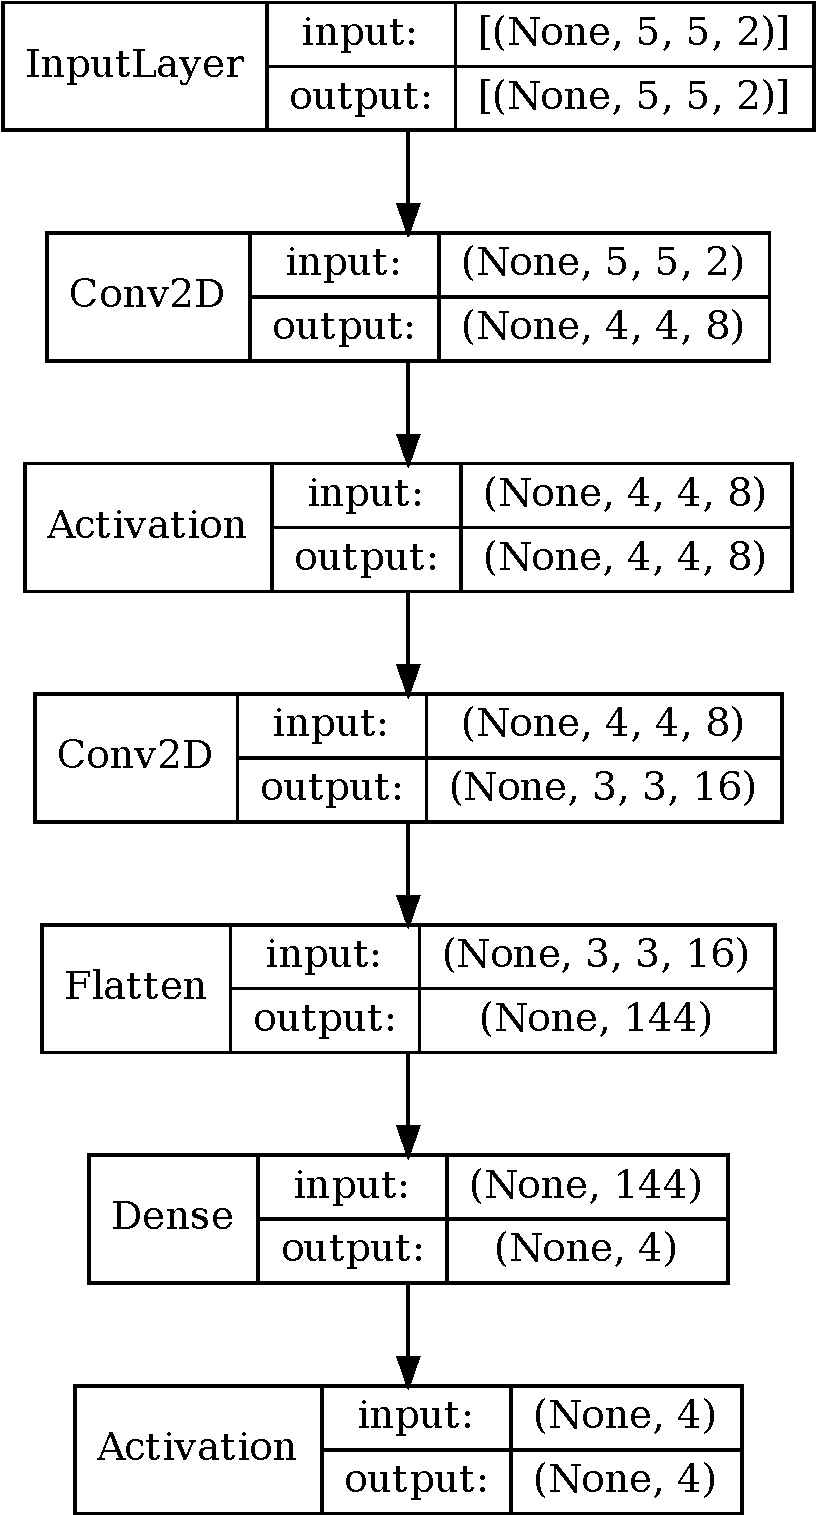
\includegraphics[width = 0.5\textwidth]{figures/dq_cnn.pdf}
		\end{figure}
		\column{0.1 \textwidth}
		\column{0.5 \textwidth}
		\begin{figure}
			\animategraphics[autoplay,loop,width=0.8\textwidth]{15}{figures/DQ/cnn_test0_}{0}{201}
		\end{figure}
	\end{columns}
\end{frame}

\begin{frame}{}{$\epsilon$-greedy Algorithm}
	The $\epsilon$-greedy algorithm is a common exploration strategy used in Deep Q learning. Balances exploration, where the agent tries out new actions and collects new data, and exploitation, where the agent uses the information it already has to select the action with the highest expected reward. The algorithm selects a random action with probability $\epsilon$ and the action with the highest Q value with probability $1-\epsilon$. The value of $\epsilon$ decreases over time to gradually shift the focus from exploration to exploitation.
\end{frame}

\begin{frame}{}{Model 2+ Incorporated $\epsilon$-exploration}

	\begin{columns}[c, onlytextwidth]
		\column{0.4 \textwidth}
		Convolutional network + $\epsilon$-greedy Algorithm during training:
		\begin{figure}
			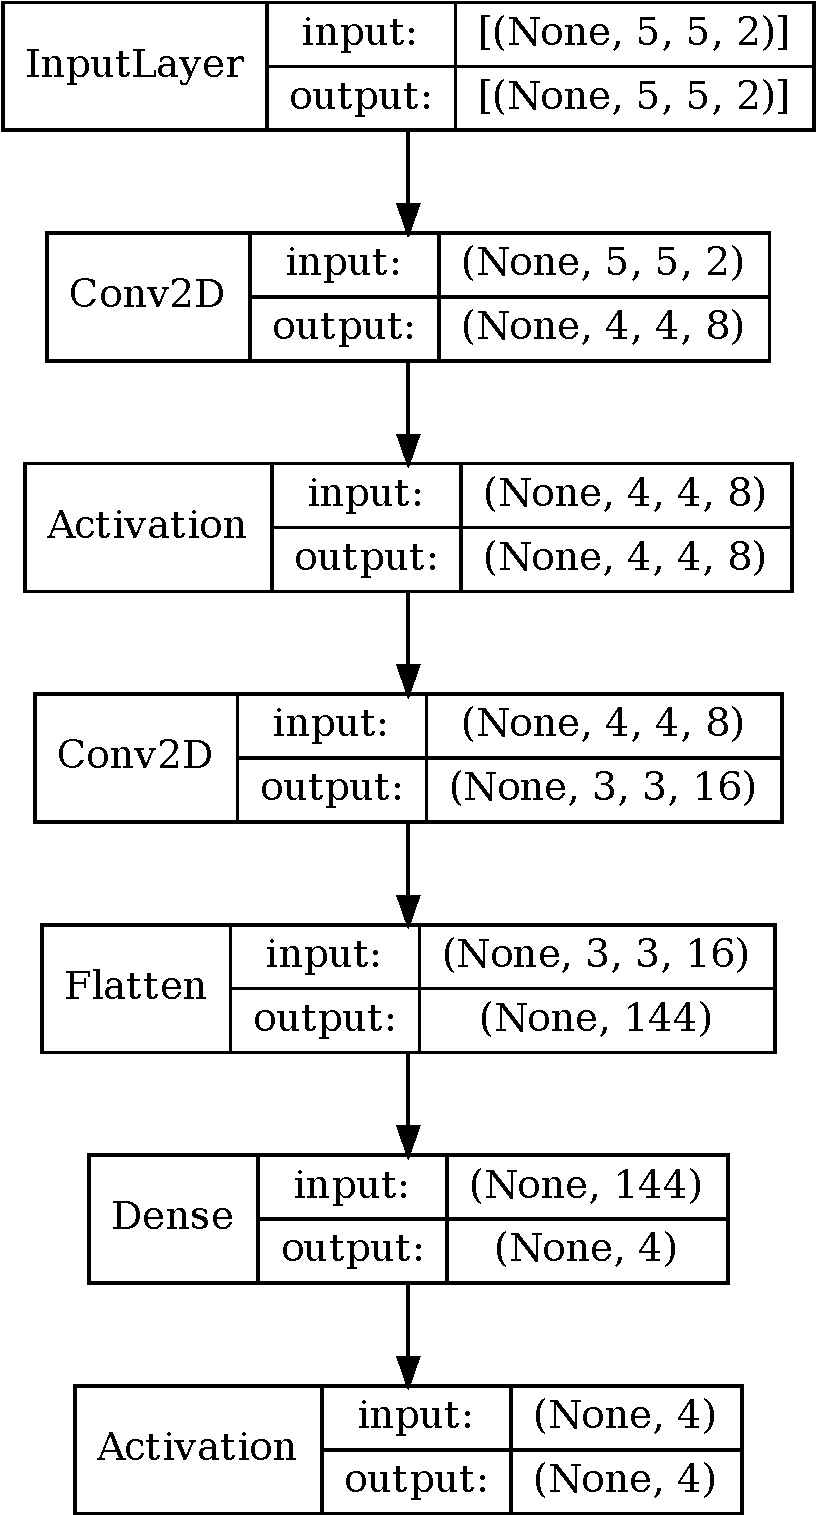
\includegraphics[width = 0.5\textwidth]{figures/dq_cnn.pdf}
		\end{figure}
		\column{0.1 \textwidth}
		\column{0.5 \textwidth}
		\begin{figure}
			\animategraphics[autoplay,loop,width=0.8\textwidth]{15}{figures/DQ/cnn_test_exp0_}{0}{201}
		\end{figure}
	\end{columns}
\end{frame}

\section{Synthetic Data Generation with Generative Adversarial Networks}
\subsection{GANS Models}
\begin{frame}
	Generative Adversarial Networks (GANs) are a type of deep learning architecture composed of two neural networks, the generator and the discriminator, that are trained in a adversarial manner. The generator network is trained to generate fake data that appears similar to real data, while the discriminator network is trained to distinguish between real and fake data. The loss for GANs is defined as a min-max game, where the generator minimizes the loss function, and the discriminator maximizes it. $D$ and $G$ represent the discriminator and generator networks, respectively, and the goal is to find the optimal configuration for $D$ and $G$ such that the generated samples appear indistinguishable from real data.

	\begin{figure}
		\centering
		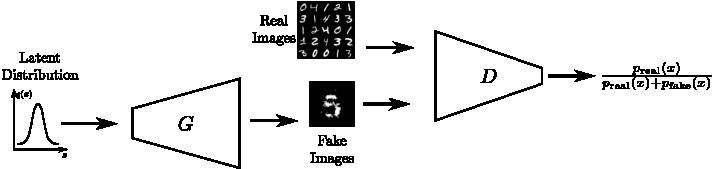
\includegraphics[width = 0.9\textwidth]{figures/GAN.pdf}
	\end{figure}
\end{frame}
\begin{frame}
	The loss of a  (GAN) is defined as a minimax game between the generator and discriminator models. The generator aims to generate samples that are indistinguishable from real samples, while the discriminator aims to distinguish the generated samples from real samples. The loss function for the generator is defined as $-\log(D(G(z)))$, where $D$ is the discriminator model and $G(z)$ is the generator's output for a random noise vector $z$. The loss function for the discriminator is defined as $\log(D(x)) + \log(1 - D(G(z)))$, where $x$ is a real sample.
	$$
		\min_D \max_G \mathbb{E}_{x\sim p_{\mathrm{real}}}\left[\log(D(x))\right]  +  \mathbb{E}_{z\sim q}\left[ \log(1 - D(G(z)))\right]
	$$

	\begin{figure}
		\centering
		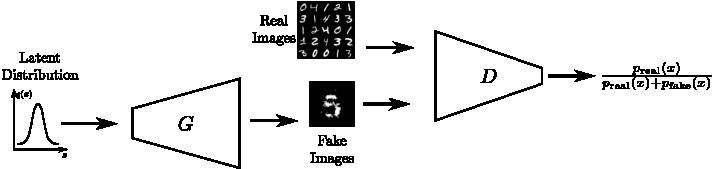
\includegraphics[width = 0.9\textwidth]{figures/GAN.pdf}
	\end{figure}
\end{frame}

\subsection{MNIST Generation}
\begin{frame}
	\begin{columns}[c, onlytextwidth]
		\column{0.5\textwidth}
		\centering $G$
		\begin{figure}
			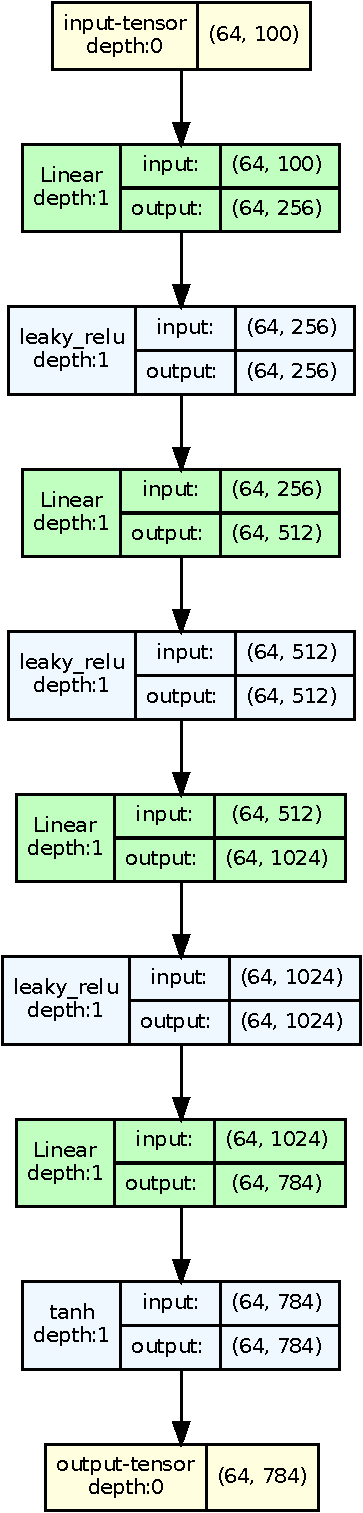
\includegraphics[width=0.2\textwidth]{figures/F.pdf}
		\end{figure}

		\column{0.5\textwidth}
		\centering $D$
		\begin{figure}
			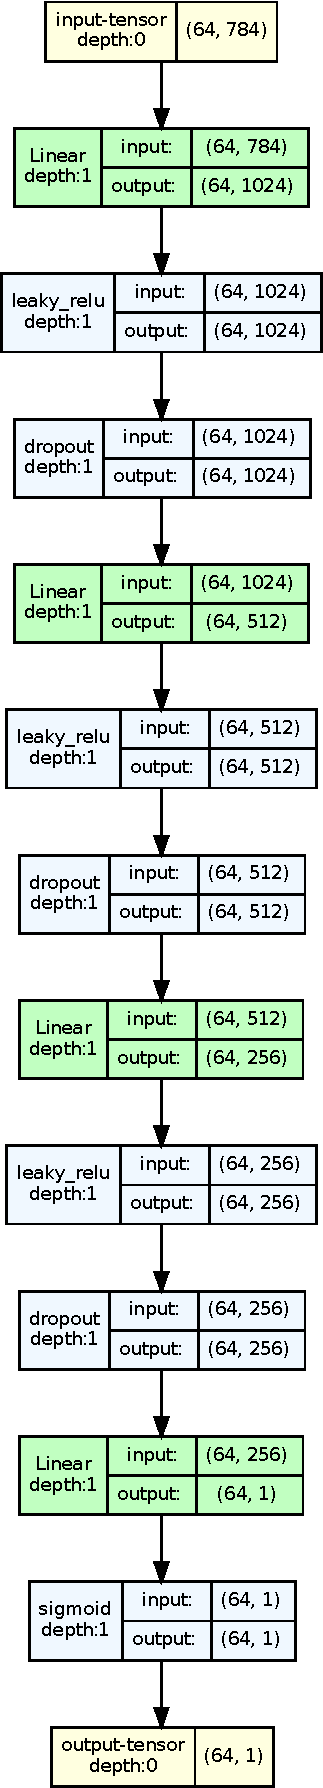
\includegraphics[width=0.2\textwidth]{figures/D.pdf}
		\end{figure}
	\end{columns}
\end{frame}

\begin{frame}
	\begin{figure}
		\centering
		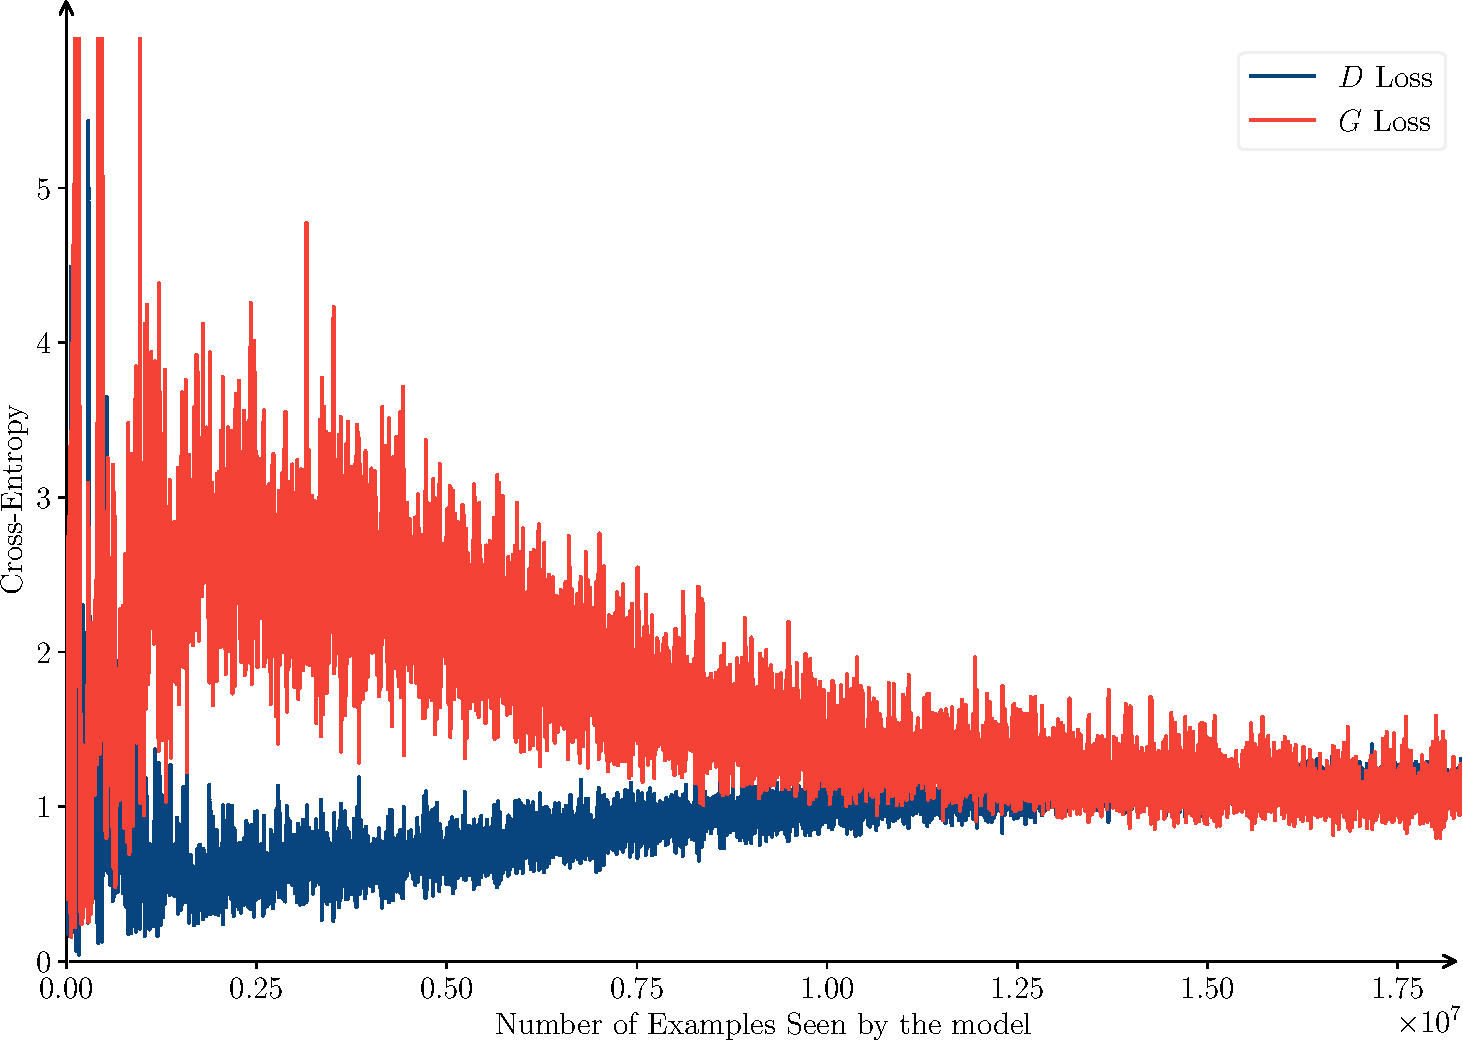
\includegraphics[width = 0.6 \textwidth]{figures/gan_loss.pdf}
	\end{figure}
\end{frame}

\begin{frame}
	\begin{figure}
		\animategraphics[autoplay,loop,width=0.4\textwidth]{15}{figures/GAN/sample_}{1}{305}
	\end{figure}
\end{frame}
\section{Sentiment Analysis with Transformers and GRU}
\subsection{Bert}
\begin{frame}
	BERT (Bidirectional Encoder Representations from Transformers) is a pre-trained language model developed by Google in 2018. It is a transformer-based architecture that uses a masked language modeling task to generate a deep understanding of the contextual relationships between words in a sentence. BERT can be fine-tuned for various NLP tasks such as sentiment classification by adding a classification layer on top of its pre-trained representations. The model has achieved state-of-the-art performance in a wide range of NLP tasks, making it a popular choice for sentiment analysis.\newline

	A bidirectional transformer is a type of transformer architecture in natural language processing (NLP) where information from both past and future contexts is taken into consideration when making predictions. This is achieved by processing the input sequence in two directions, starting from the beginning and the end of the sequence, and concatenating the outputs to obtain the final representation. This allows the model to capture the context both in the forward and backward directions, providing a more comprehensive representation of the input sequence.
\end{frame}


\begin{frame}
	BERT model consists of multiple transformer encoder blocks, with a self-attention mechanism, a feedforward neural network and layer normalization, stacked on top of each other. It also includes a positional encoding component to capture the relative position of tokens in a sequence, and a segment encoding component to differentiate between different sequences within the same input.
	\begin{figure}
		\centering
		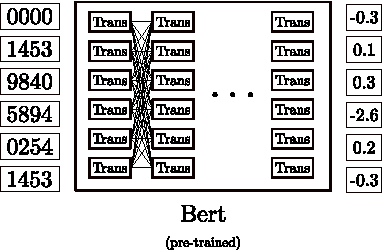
\includegraphics[width = 0.6 \textwidth]{figures/bert.pdf}
	\end{figure}
\end{frame}
\begin{frame}{}{Training Bert}

	Bert is trained on two tasks, the masked language model and the next sentence prediction. In the masked language model task, a portion of the input sequence is masked and the model must predict the original token based on its context. In the next sentence prediction task, the model receives a pair of sentences and must predict whether the second sentence follows the first one in the context of the input text. Both of these tasks are used to train Bert to understand the context of words in a sentence and how they relate to each other, allowing it to perform well on a wide range of natural language processing tasks.
	\begin{figure}
		\centering
		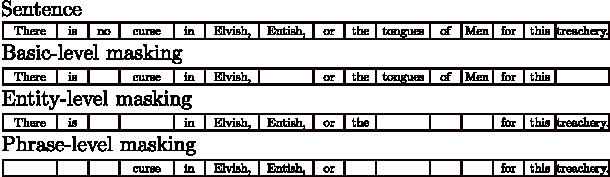
\includegraphics[width = 0.8 \textwidth]{figures/masking.pdf}
	\end{figure}
\end{frame}
\subsection{Sentiment Analysis}
\begin{frame}
	Bert can be fine-tuned for sentiment analysis by adding a classifier layer on top of the pretrained Bert model. The layer is trained on a labeled sentiment analysis dataset to predict the sentiment of a given input sequence, which can be a sentence, paragraph, or document. Fine-tuning the model allows it to learn the specific nuances of sentiment in the target task and produce improved results compared to using the pre-trained model alone.
	\begin{figure}
		\centering
		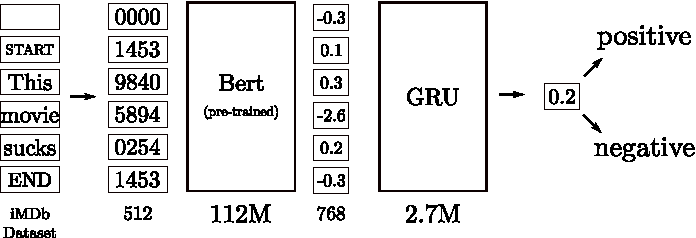
\includegraphics[width = 0.6 \textwidth]{figures/Bertsentiment.pdf}
	\end{figure}
\end{frame}
\begin{frame}
	\begin{figure}
		\centering
		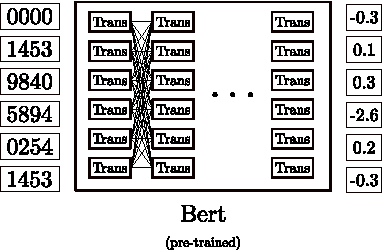
\includegraphics[width = 0.6 \textwidth]{figures/bert.pdf}
	\end{figure}
\end{frame}
\begin{frame}
	\begin{figure}
		\centering
		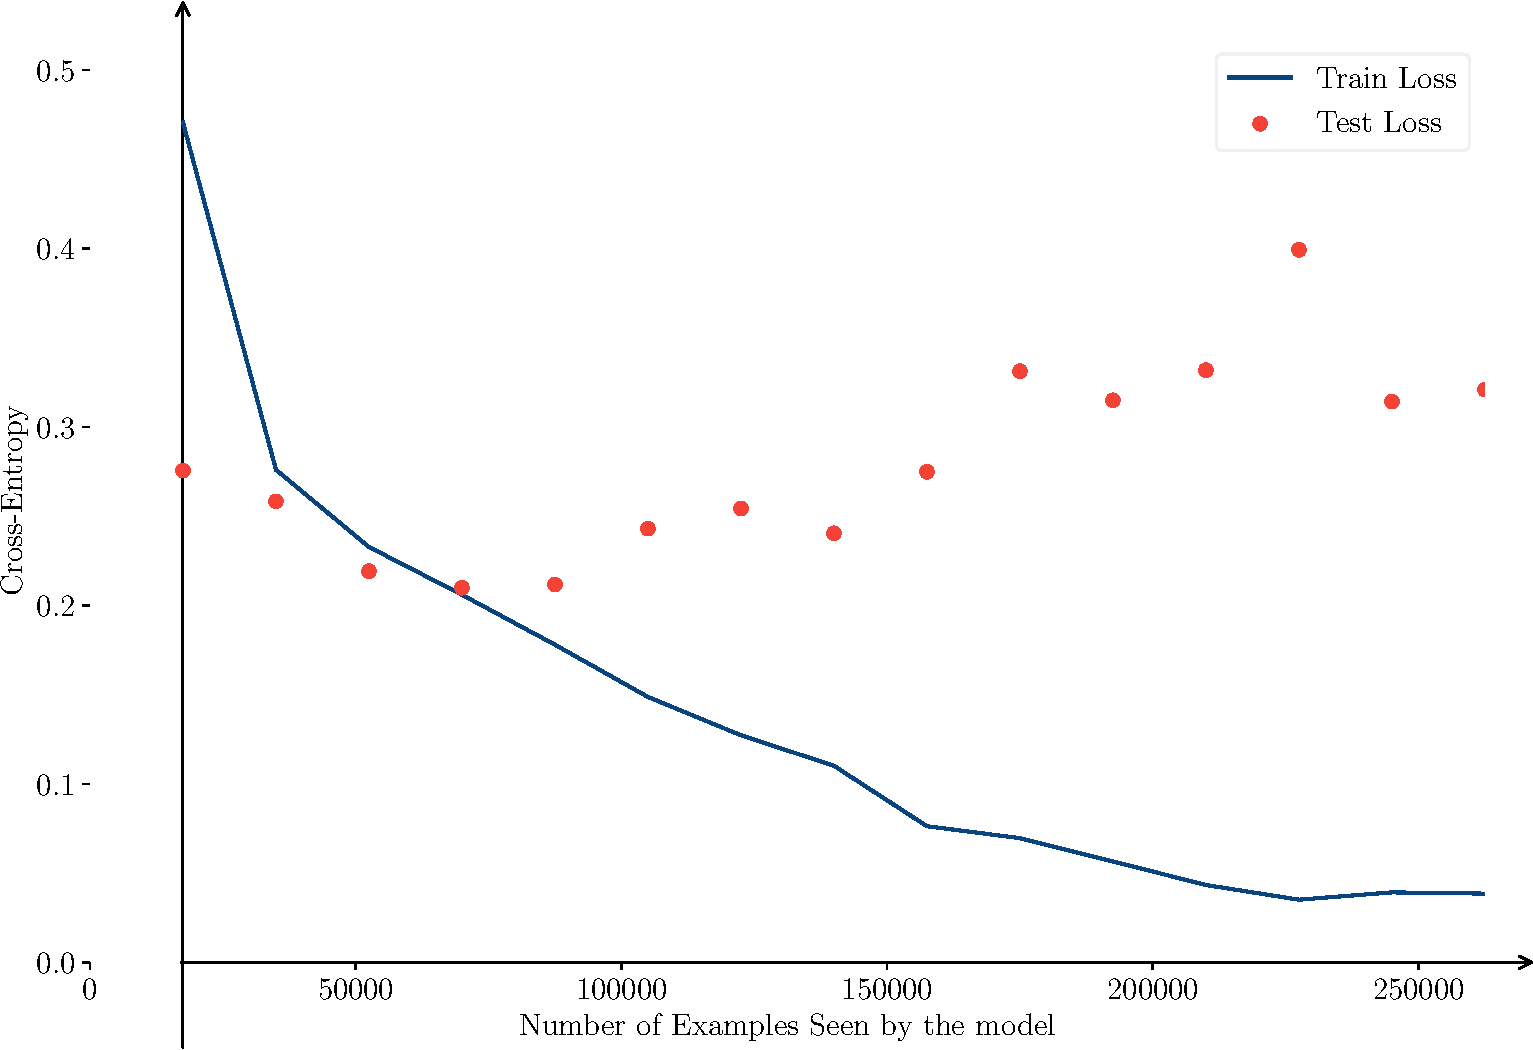
\includegraphics[width = 0.6 \textwidth]{figures/bert_res.pdf}
	\end{figure}
\end{frame}

\begin{frame}
	\begin{figure}
		\centering
		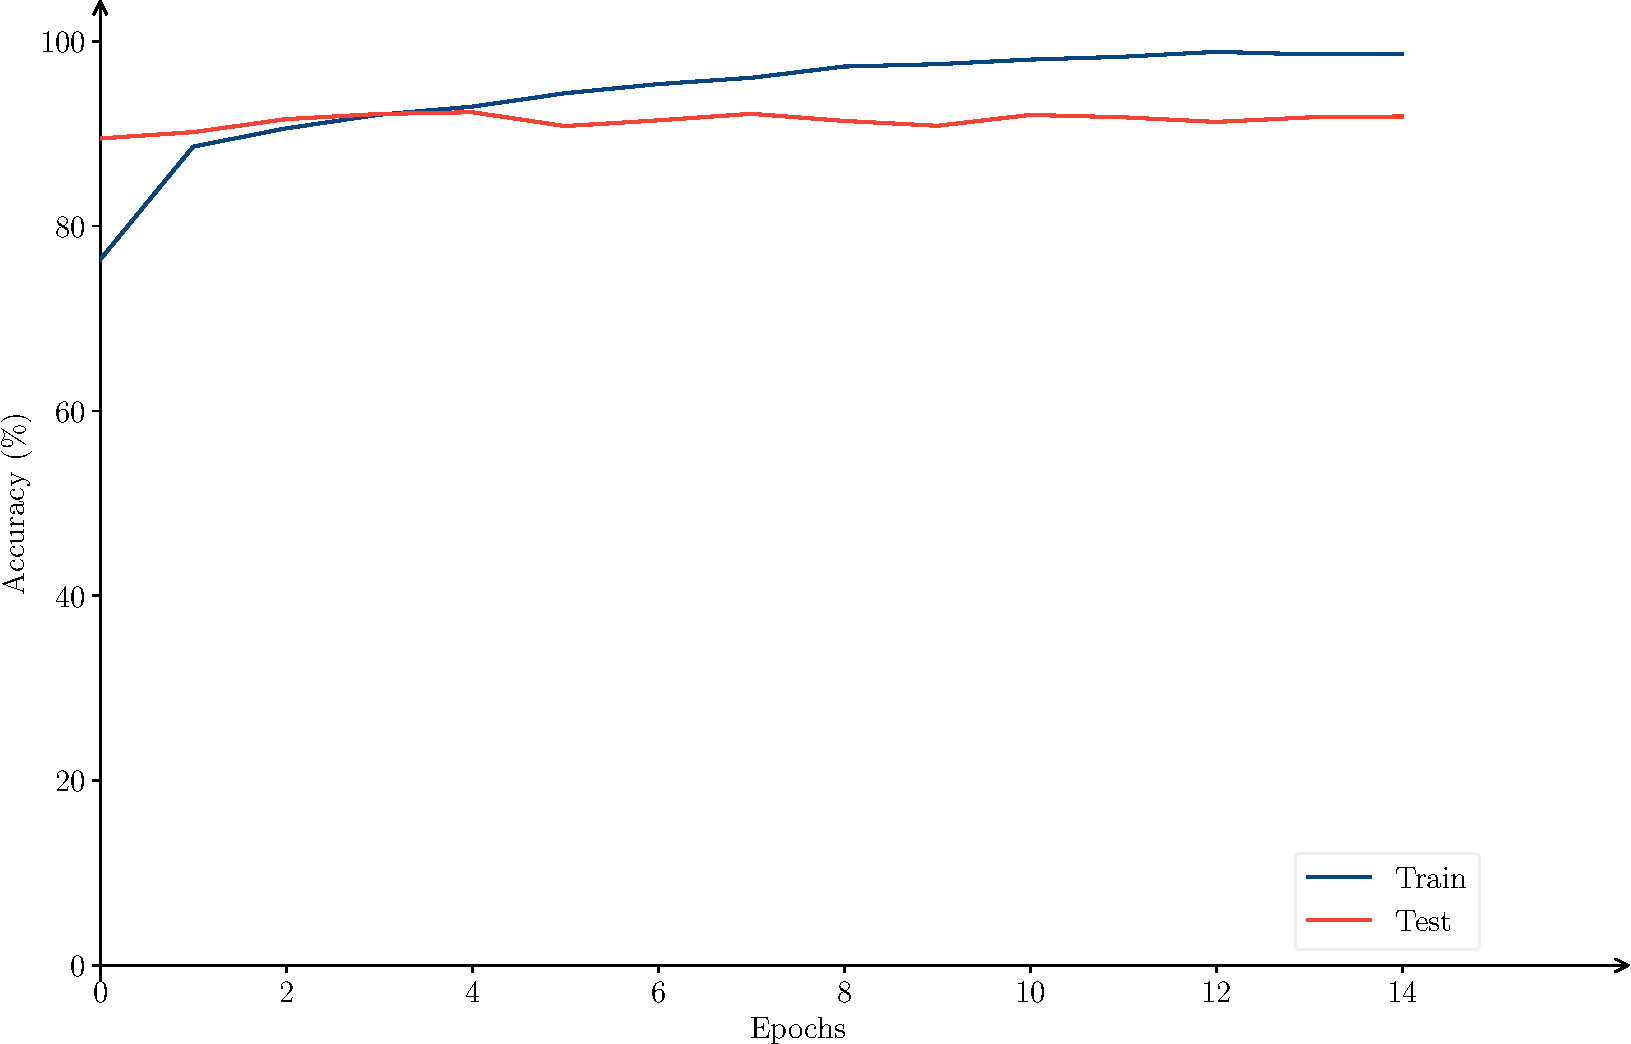
\includegraphics[width = 0.6 \textwidth]{figures/bert_acc.pdf}
	\end{figure}
\end{frame}

\begin{frame}
	\begin{figure}
		\centering
		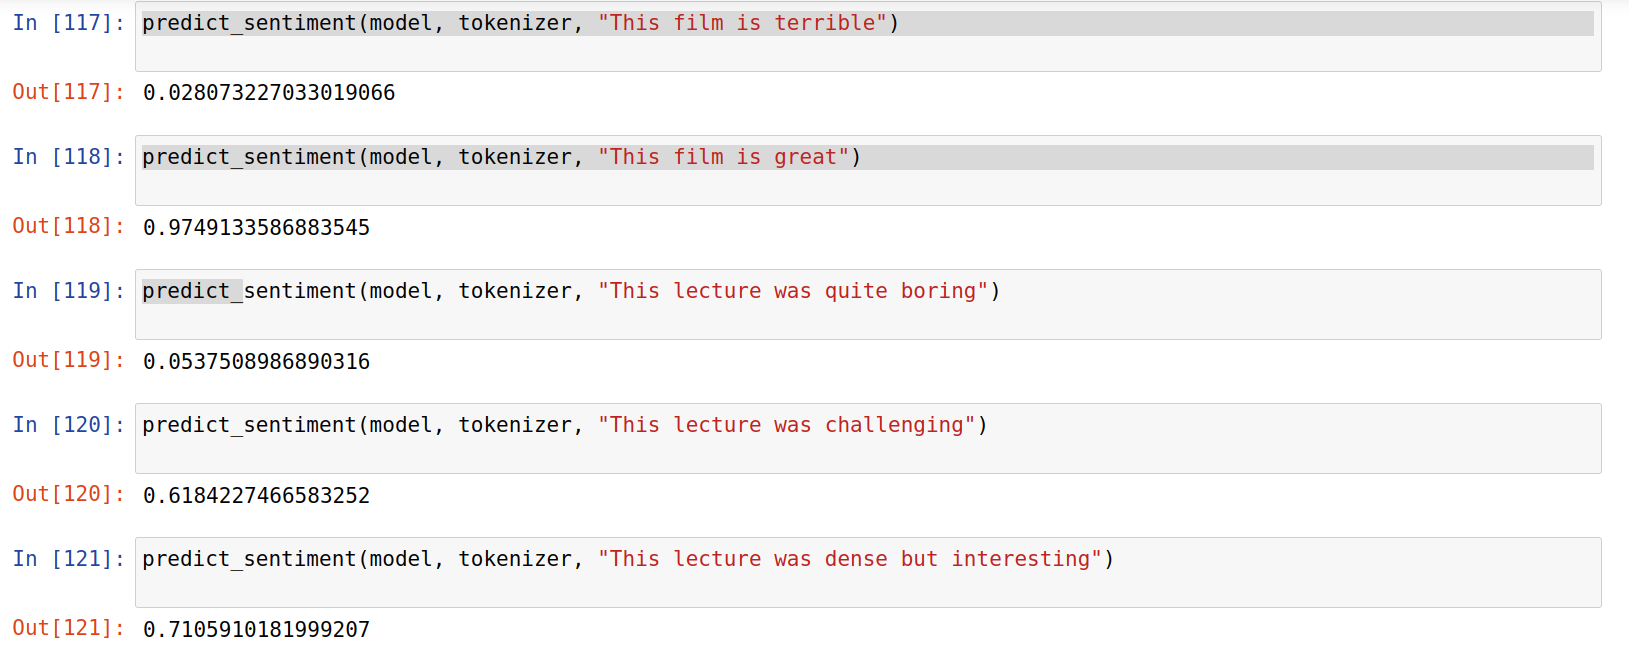
\includegraphics[width = 0.7 \textwidth]{figures/bert_sen.png}
	\end{figure}
\end{frame}





\section{Density Estimation with Normalizing Flows}
\subsection{Estimating Density}
\begin{frame}
	In Machine Learning, the task of \emph{density estimation} consists in estimating the probability density function of a random variable from a set of observations. This is a fundamental problem in statistics and machine learning, with applications in a wide range of fields, including anomaly detection, clustering, and generative modeling. There are several methods for density estimation, including parametric models, non-parametric models, and deep learning models. In this section, we will focus on a specific type of deep learning model called Normalizing Flows, which is used for density estimation and generative modeling.
	\vskip 5pt
	\begin{figure}
		\centering
		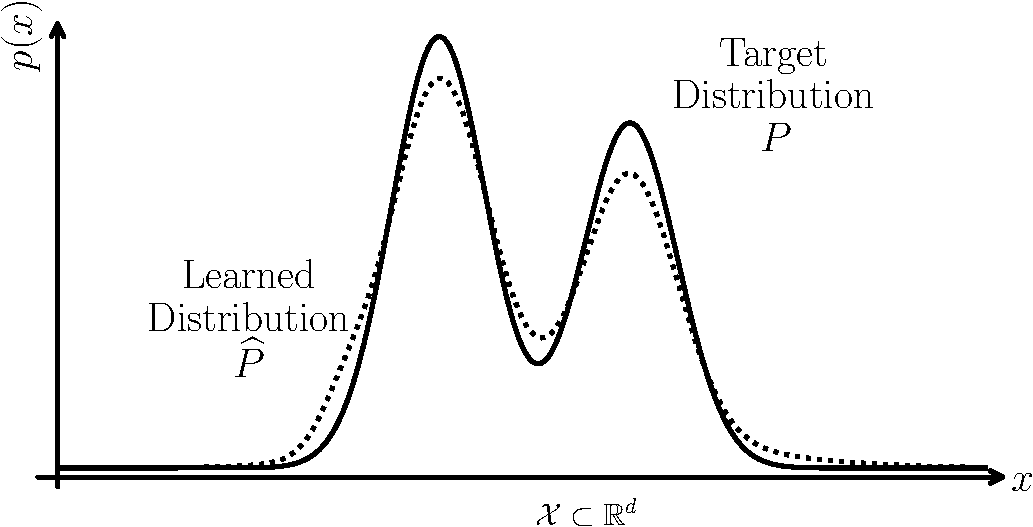
\includegraphics[width = 0.5\textwidth]{figures/targetnproposal.pdf}
	\end{figure}

\end{frame}

\subsection{Normalizing Flows}




\begin{frame}{}{Overview}
	A Normalizing Flow is usually seen as:
	\begin{itemize}
		\item a  {\em generative model},
		\item a {\em bijective mapping},
		\item an {\em invertible neural network},
		\item a {\em density estimator}.
	\end{itemize}
\end{frame}
\begin{frame}{}{Overview}
	\begin{figure}
		\centering
		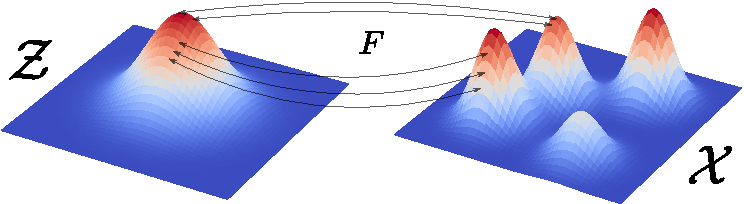
\includegraphics[width = \textwidth]{figures/Distribution_NF.pdf}
		\caption{A mapping between two probability distributions\\Point to point}
	\end{figure}
\end{frame}
\begin{frame}{}{Overview}
	\begin{figure}
		\centering
		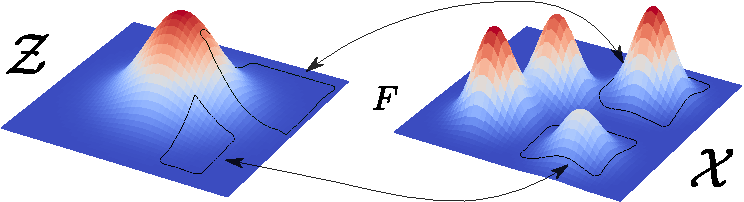
\includegraphics[width = \textwidth]{figures/Distribution_NF2.pdf}
		\caption{A mapping between two probability distributions\\Subset to subset}
	\end{figure}
\end{frame}

\begin{frame}{}{Mathematical Framework}
	\begin{block}{Normalizing Flow}
		A Normalizing Flow is a bijective function between a data space $\mathcal{X}$ and a latent space $\mathcal{Z}$, both subset of $\mathbb{R}^d$.
		$$
			\begin{array}{rccl}
				F : & \mathcal{X} & \longmapsto & \mathcal{Z} \\
				    & x           & \longmapsto & z = F(x)
			\end{array}
		$$
	\end{block}
	\begin{block}{Data and Latent Distributions}
		In theory, a NF maps a target distribution $P$, ie the data distribution to a  simple latent distribution $Q$.
	\end{block}
	Usually, $Q$ is set to be a Normal Gaussian multivariate distribution $\mathcal{N}(0_d,I_d)$. $p$ and $q$ are respectivelly the probability densities of $P$ and $Q$.
\end{frame}

\begin{frame}{}{How does it work ?}
	In practice, the mapping is {\em  not perfect}. $P^*$ induces a distribution $Q$ and similarly, the latent distribution $Q$ induces $\widehat P$,  which is the learned distribution. The forward pass $F$ is called the {\em Normalizing } direction while the inverse pass $F^{-1}$ is called the {\em Generative} direction.
	\vskip 5pt
	\begin{figure}
		\centering
		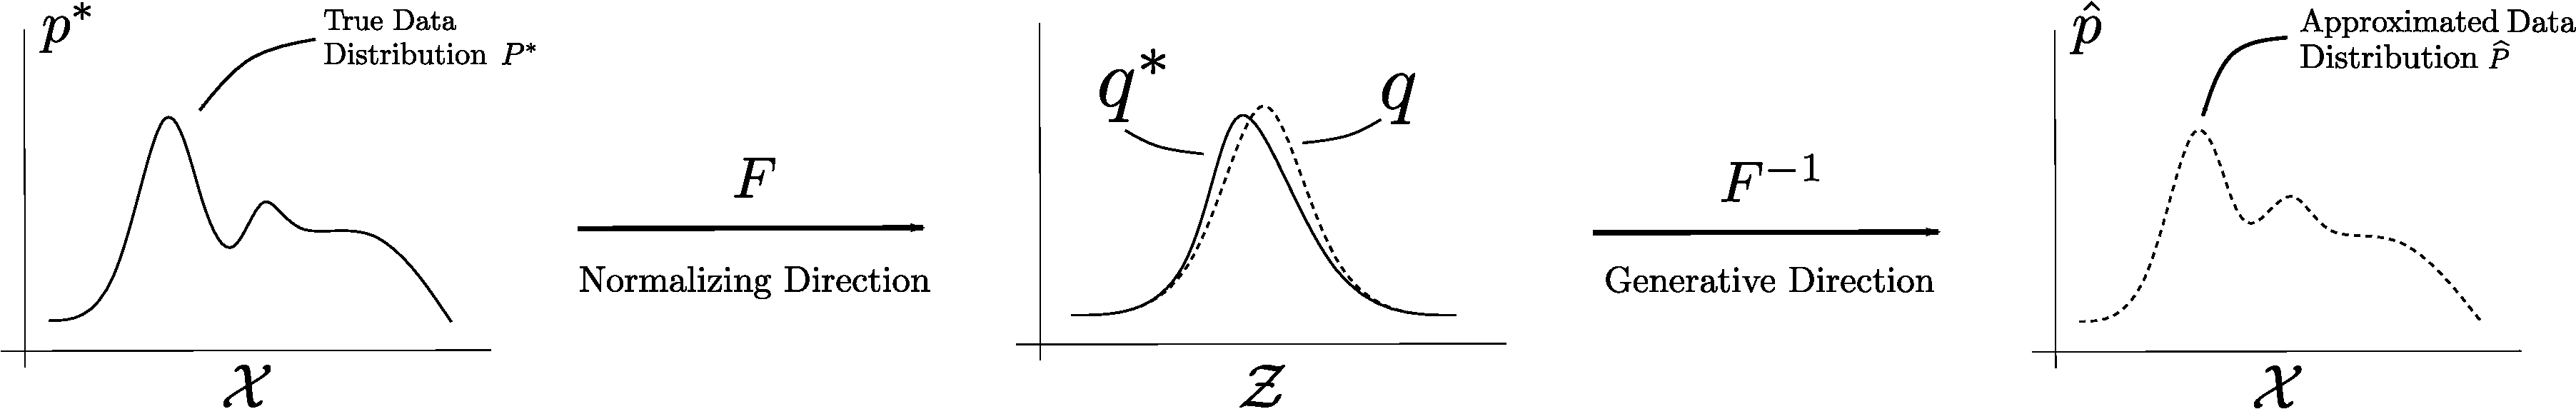
\includegraphics[width = \textwidth]{figures/nf.pdf}
		\caption{1D Normalizing Flow process.}
	\end{figure}
\end{frame}

\begin{frame}{}{Induced Probabilities ? }
	\begin{block}{Change of Variable Formula}
		For a bijective and continuous fonction $F$ and a latent distribution $Q$, the distribution induced by $Q$ and $F$ is defined through the {\em change of variable formula}:
		\begin{equation}
			\label{eq:cov}
			\forall x \in \mathcal{X}, \quad \hat p(x) = \vert \det \mathrm{Jac}_F(x)\vert ~ q(F(x)).
		\end{equation}
	\end{block}
\end{frame}

\begin{frame}{}{Induced Probabilities ? }
	$$\forall x \in \mathcal{X}, \quad \hat p(x) = \vert \det \mathrm{Jac}_F(x)\vert ~ q(F(x)).$$
	\only<1>{
		\begin{figure}
			\centering
			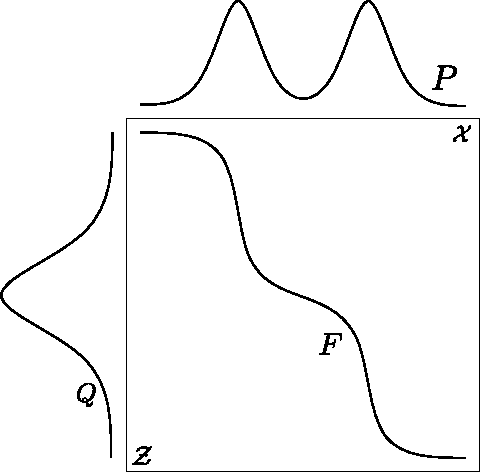
\includegraphics[width = 0.4\textwidth]{figures/monge.pdf}
		\end{figure}
	}
	\only<2>{
		\begin{figure}
			\centering
			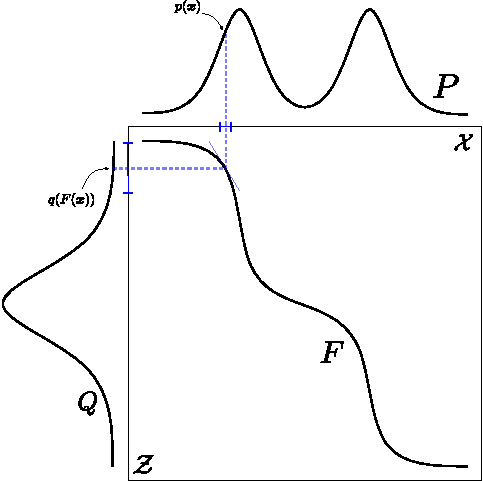
\includegraphics[width = 0.4\textwidth]{figures/monge_L1.pdf}
		\end{figure}
	}
	\only<3>{
		\begin{figure}
			\centering
			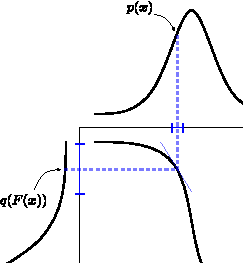
\includegraphics[width = 0.4\textwidth]{figures/monge_L1_cropped.pdf}
		\end{figure}
	}
	\only<4>{
		\begin{figure}
			\centering
			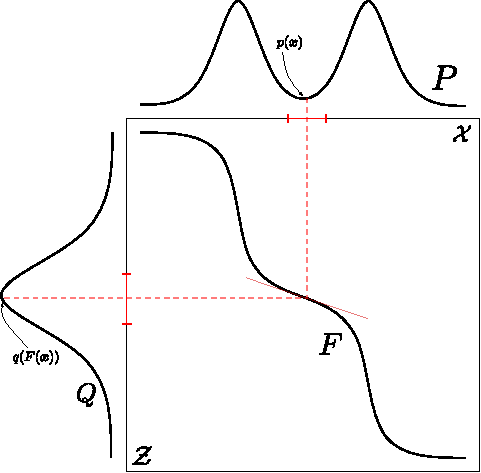
\includegraphics[width = 0.5\textwidth]{figures/monge_L2.pdf}
		\end{figure}
	}
	\only<5>{
		\begin{figure}
			\centering
			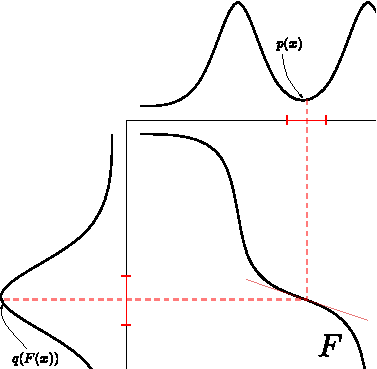
\includegraphics[width = 0.4\textwidth]{figures/monge_L2_cropped.pdf}
		\end{figure}
	}

\end{frame}

\begin{frame}{}{Density Estimation}
	To perfom density estimation:
	\begin{enumerate}
		\item Draw $x \sim P^*$,
		\item Compute $F(x)$ and $\vert \det \mathrm{Jac}_F(x)\vert$,
		\item Compute $\widehat{p}(x) = q(F(x))\vert \det \mathrm{Jac}_F(x)\vert $.
	\end{enumerate}
	\begin{figure}
		\centering
		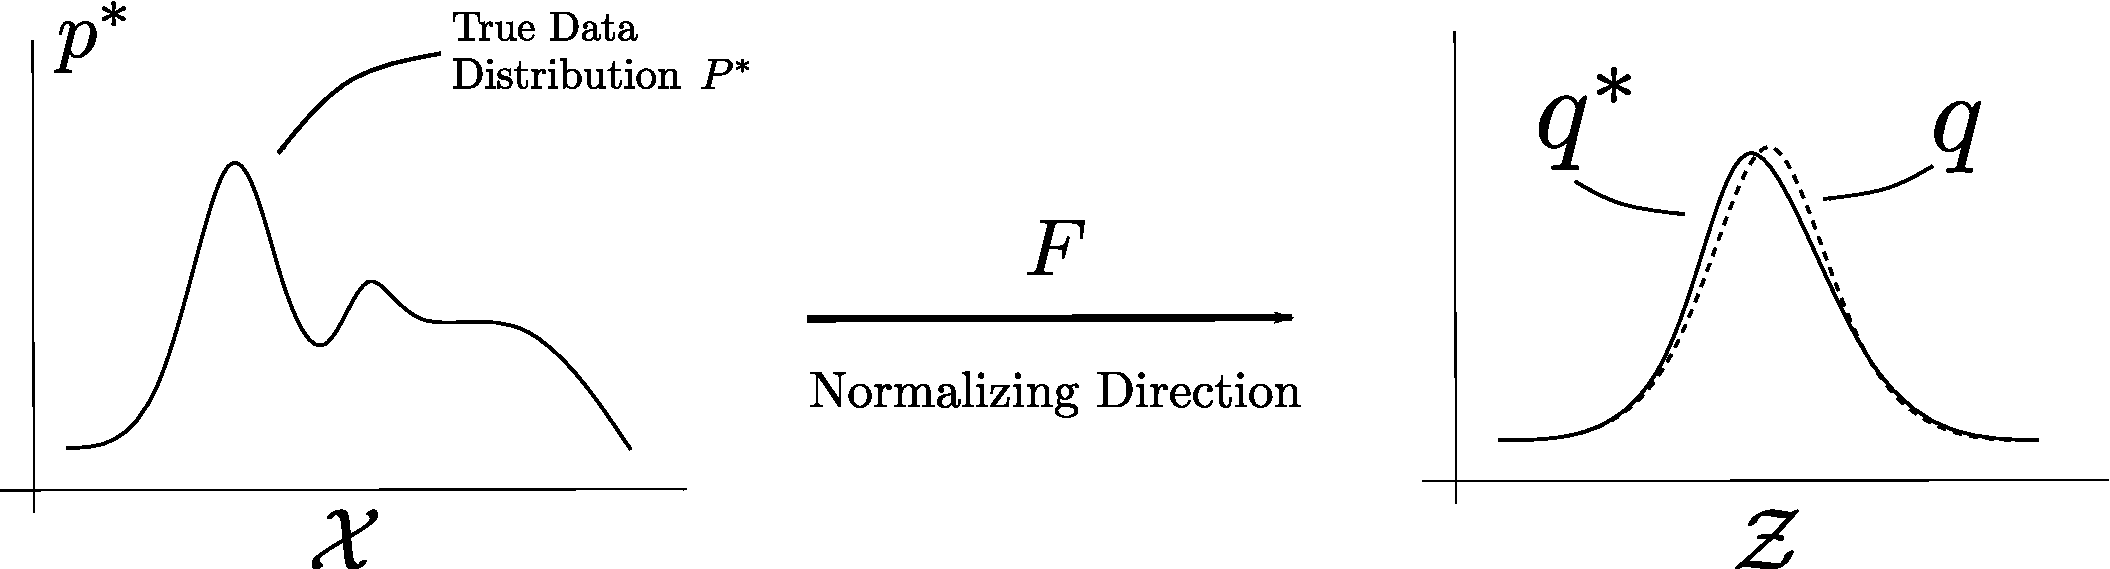
\includegraphics[width = 0.9\textwidth]{figures/nf_de.pdf}
		\caption{1D Normalizing Process of Density Estimation.}
	\end{figure}
\end{frame}

\begin{frame}{}{Data Generation}
	To perform data generation:
	\begin{enumerate}
		\item Draw $z \sim Q$,
		\item Compute $x = F^{-1}(x)$.
	\end{enumerate}
	\begin{figure}
		\centering
		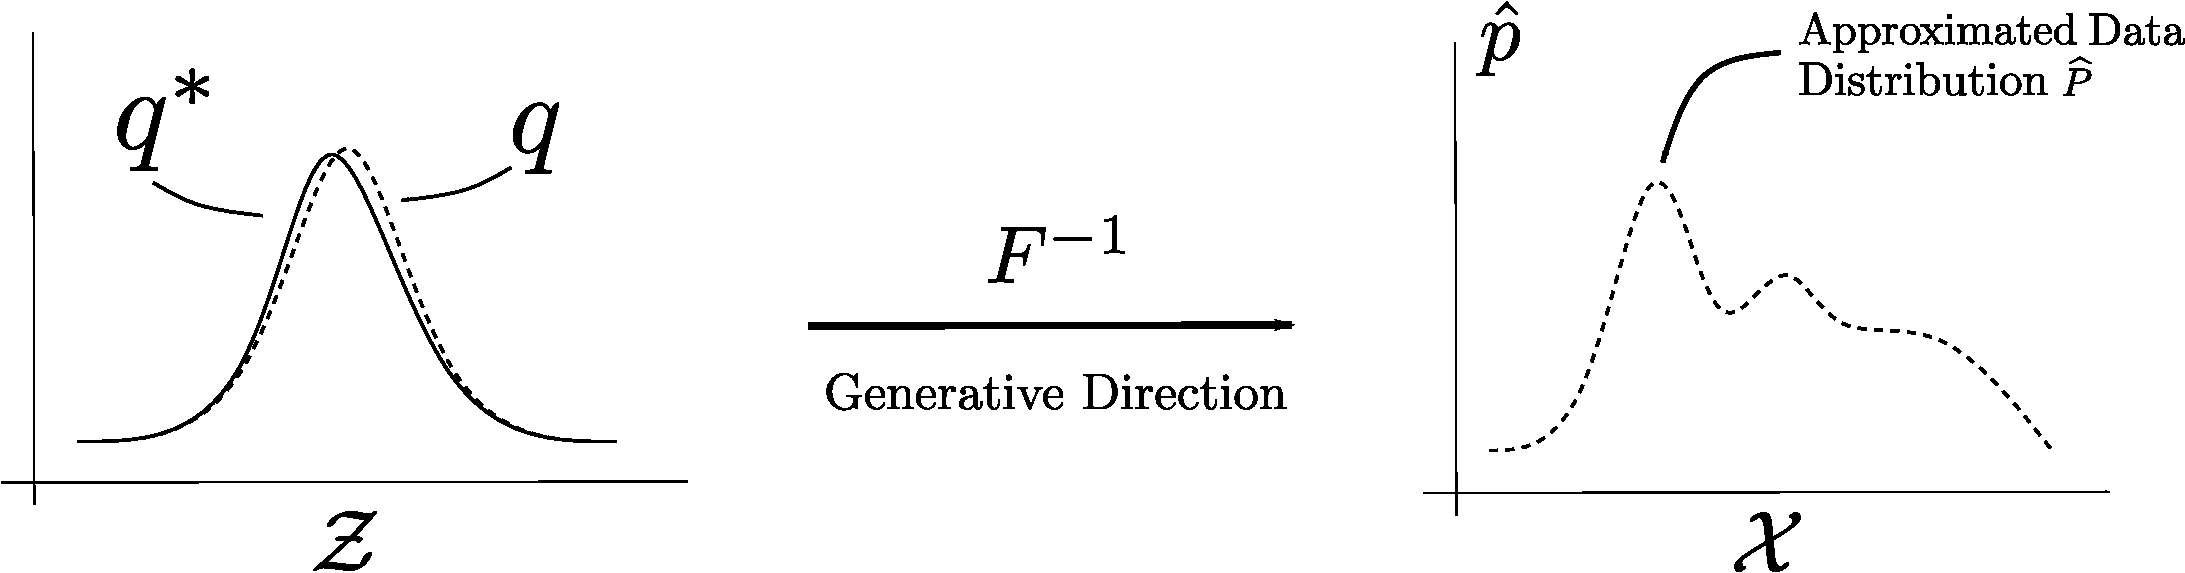
\includegraphics[width = 0.9\textwidth]{figures/nf_gen.pdf}
		\caption{1D Normalizing Flow process of Generation.}
	\end{figure}
\end{frame}



\begin{frame}{}{Log-Likelihood}
	\begin{exampleblock}{Loss}
		The objective is to approximate $P^*$ with $\widehat P$. We can minimize the Kullback-Leiber Divergence :
		\begin{equation*}
			\theta = \argmin_\theta \mathcal{D}_{\mathrm{KL}}(P^*\Vert \widehat{P}).
		\end{equation*}
		This is equivalent to maximizing the log likelihood :
		\begin{equation*}
			\theta = \argmax_\theta \mathbb{E}_{x\sim \mathcal{X}} \left[\log\widehat{p}(x)\right].
		\end{equation*}
	\end{exampleblock}
\end{frame}

\begin{frame}{}{Log-Likelihood}
	$$ \mathcal{D}_{\mathrm{KL}}(P^*\Vert \widehat{P}) = \int_{\mathcal{X}}p^*(x)\log\left(\frac{p^*(x)}{\widehat p(x)}\right)dx$$
	\vfill
	\vskip 75pt
	$$ \mathrm{nll} =- \mathbb{E}_{x\sim\mathcal{X}}\left[\log \widehat p (x)\right]$$
\end{frame}

\begin{frame}{}{Learning steps}
	\begin{figure}
		\centering
		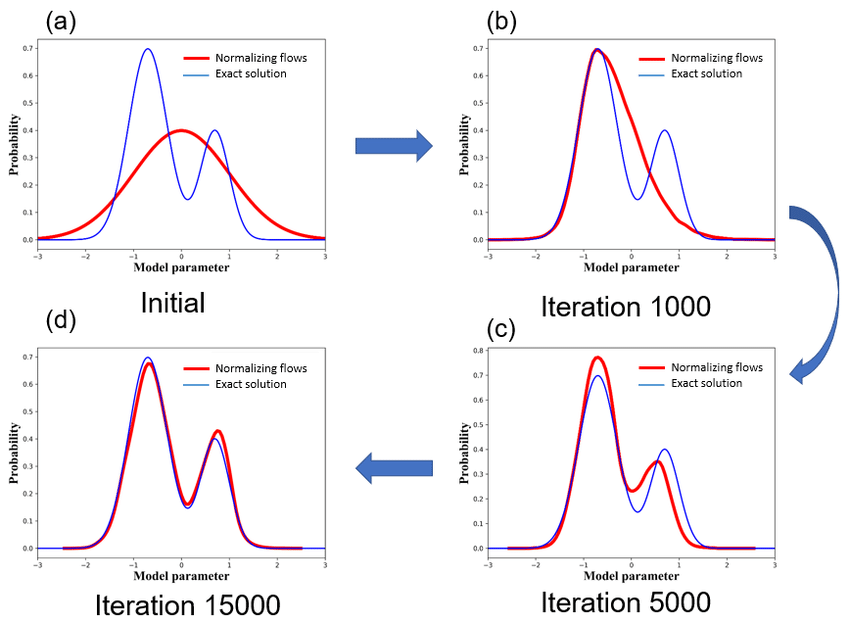
\includegraphics[width = 0.65\textwidth]{figures/learning.png}
		\caption{Learning Process for a 1D Normalizing Flow.}
	\end{figure}
\end{frame}


\section{Image Segmentation with U-Net}
\subsection{Image Segmentation}

\begin{frame}
	Image segmentation is the process of partitioning an image into multiple segments or regions based on the characteristics of the pixels. It is a fundamental task in computer vision and has applications in various fields, including medical imaging, autonomous driving, and satellite image analysis. There are several methods for image segmentation, including thresholding, clustering, and deep learning-based approaches. In this section, we will focus on a deep learning model called U-Net, which is commonly used for image segmentation tasks.

	\begin{figure}
		\centering
		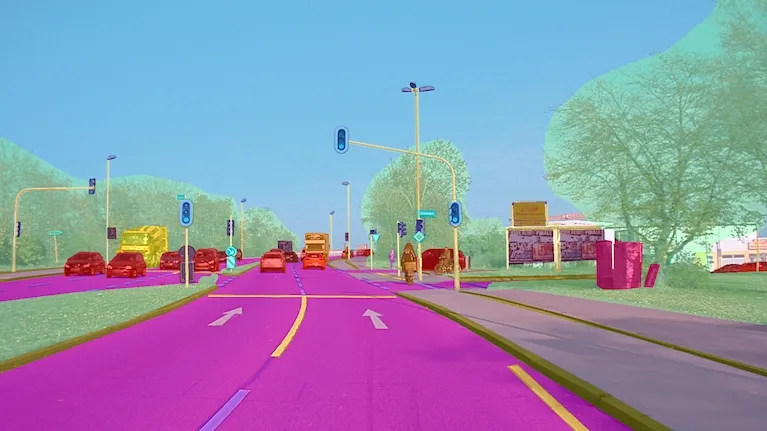
\includegraphics[width = 0.6\textwidth]{figures/imageseg.png}
	\end{figure}
\end{frame}

\begin{frame}{}{Applications of Image Segmentation}
	Image segmentation has a wide range of applications in computer vision and image processing, including:
	\begin{itemize}
		\item Medical Imaging: Segmentation of organs, tumors, and other structures in medical images.
		\item Autonomous Driving: Segmentation of objects such as cars, pedestrians, and road signs in images captured by autonomous vehicles.
		\item Satellite Image Analysis: Segmentation of land cover types, buildings, and other features in satellite images.
		\item Object Detection: Segmentation of objects in images to localize and classify them.
		\item Image Editing: Segmentation of objects for image editing tasks such as background removal and image compositing.
	\end{itemize}
\end{frame}

\begin{frame}{}{Type of Segmentations}
	\begin{minipage}[t]{0.48\textwidth}

		Image segmentation can be broadly classified into two types: semantic segmentation and instance segmentation.
		\begin{itemize}
			\item \textbf{Semantic Segmentation:} Semantic segmentation assigns a class label to each pixel in an image, such as road, car, person, etc. The goal is to partition the image into semantically meaningful regions.
			\item \textbf{Instance Segmentation:} Instance segmentation goes a step further than semantic segmentation by distinguishing between different instances of the same class. It assigns a unique label to each object instance in the image.
		\end{itemize}
	\end{minipage}
	\hfill
	\begin{minipage}[t]{0.48\textwidth}
		\begin{figure}
			\centering
			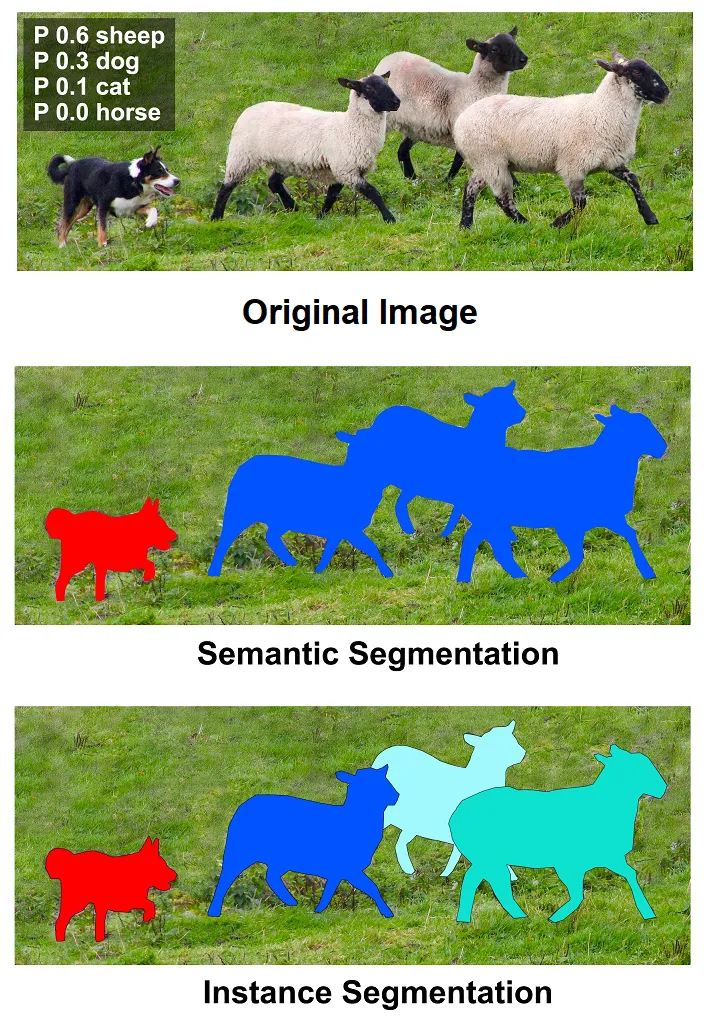
\includegraphics[width = 0.6\textwidth]{figures/typeseg.png}
		\end{figure}
	\end{minipage}
\end{frame}

\subsection{U-Net Architecture}
\begin{frame}
	U-Net is a convolutional neural network architecture designed for image segmentation tasks. It consists of an encoder-decoder structure with skip connections that allow the model to capture both local and global features in the input image.
	\begin{figure}
		\centering
		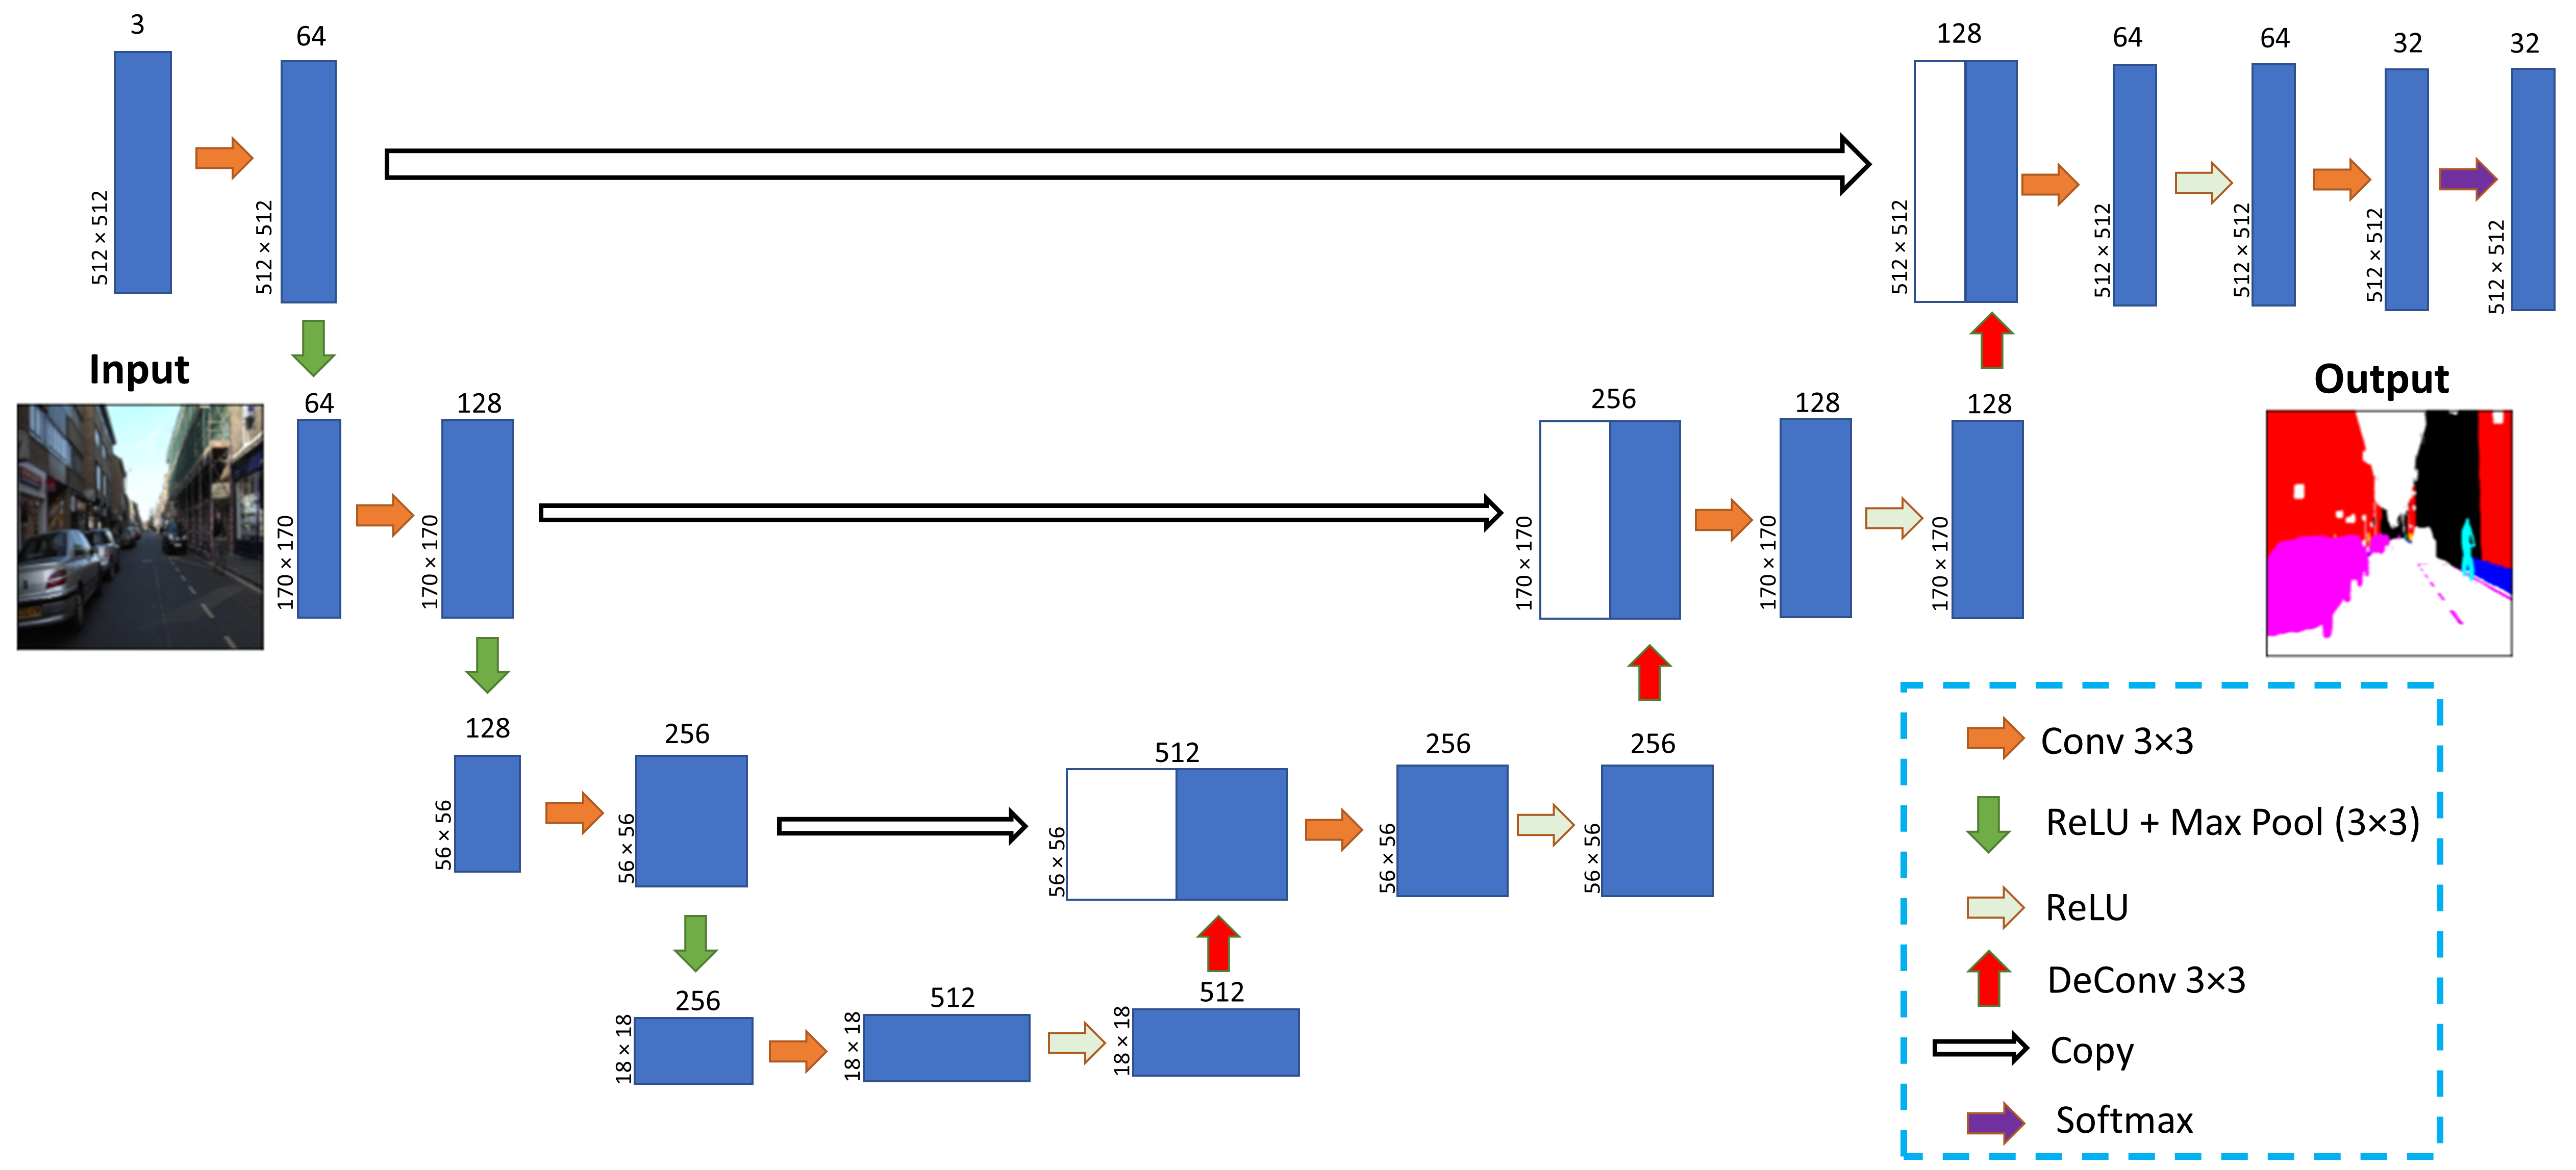
\includegraphics[width = 0.6\textwidth]{figures/U_Net_arch.png}
	\end{figure}
\end{frame}

\begin{frame}{}{Loss Functions}
	3 main loss functions are used for image segmentation tasks:
	\begin{itemize}
		\item \textbf{Categorical Cross-Entropy Loss:} Used for multi-class segmentation tasks where each pixel is classified into one of multiple classes.
		      \only<2>{
		      $$\mathcal{L} = -\frac{1}{N}\sum_{i=1}^{N}\sum_{c=1}^{C}y_{i,c}\log(\hat{y}_{i,c})$$
		      }
		\item \textbf{Dice Loss:} A similarity-based loss function that measures the overlap between the predicted segmentation mask and the ground truth mask.
		      \only<3>{
			      $$\mathcal{L} = 1 - \frac{2\sum_{i=1}^{N}y_i\hat{y}_i}{\sum_{i=1}^{N}y_i + \sum_{i=1}^{N}\hat{y}_i}$$
		      }
		\item \textbf{Shaped aware Loss:} A loss function that penalizes the model for making errors near the object boundaries, where the segmentation is most critical.
		      \only<4>{
		      $$\mathcal{L} = -w(x)\left[\frac{1}{N}\sum_{i=1}^{N}\sum_{c=1}^{C}y_{i,c}\log(\hat{y}_{i,c})\right]$$
		      with $w(x)$ a weight function that assigns higher weights to pixels near the object boundaries.
		      }
	\end{itemize}
\end{frame}



\makepart{Your turn: Hands-on Deep Learning}

\section{Build and use an autoencoder}

\subsection{Formal introduction of an autoencoder}


\begin{frame}


    \begin{block}{Definition}
        An autoencoder is a type of artificial neural network used to learn efficient codings of unlabeled data. It consists of two main components:
        \begin{itemize}
            \item An \alert{encoder} function: $encoder(x): \mathbb{R}^d \rightarrow \mathbb{R}^m$ \\
                  Maps an input $x$ from the input space $\mathbb{R}^d$ to a hidden representation space $\mathbb{R}^m$.
            \item A \alert{decoder} function: $decoder(z): \mathbb{R}^m \rightarrow \mathbb{R}^d$ \\
                  Maps the hidden representation $z$ back to the original input space $\mathbb{R}^d$.
        \end{itemize}
    \end{block}

    \begin{block}{Goal}
        The primary goal of an autoencoder is to learn a representation (encoding) for a set of data, typically for the purpose of dimensionality reduction or feature learning. Through training, the autoencoder learns to compress the data from $\mathbb{R}^d$ to $\mathbb{R}^m$ (where $m < d$) and then reconstruct the data back to $\mathbb{R}^d$ as accurately as possible. This process forces the autoencoder to capture the most important features of the data in the hidden representation $z$.
    \end{block}
\end{frame}

\begin{frame}
    \begin{figure}
        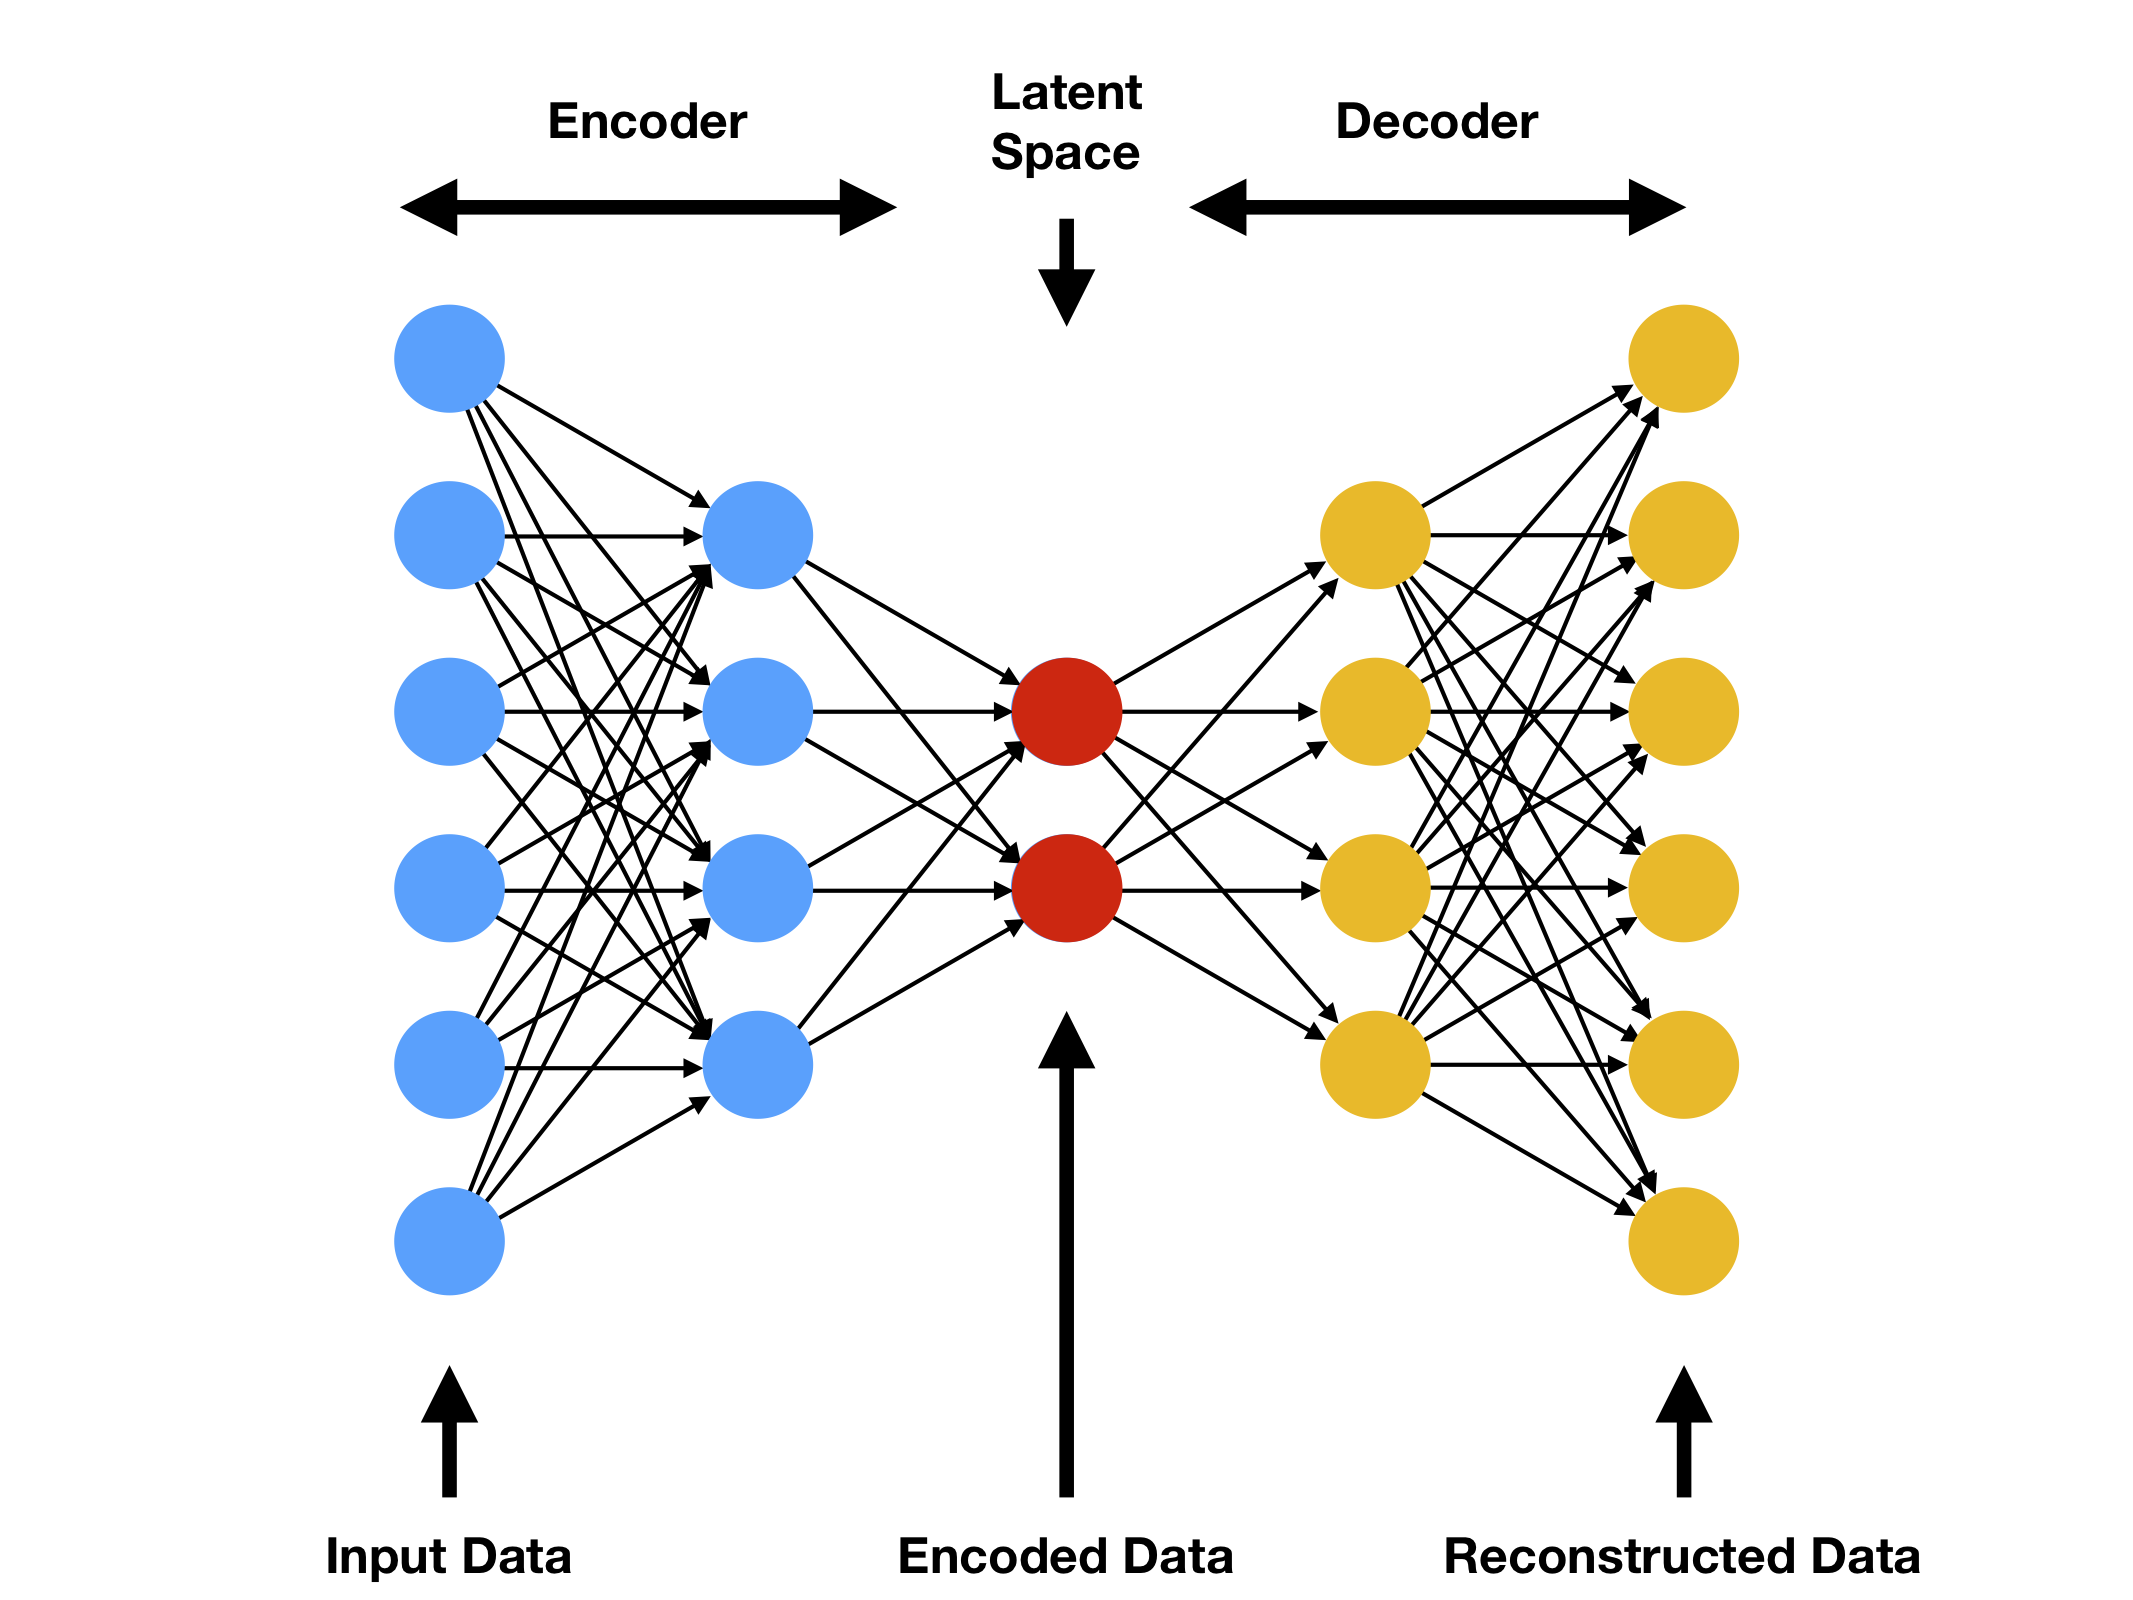
\includegraphics[width=0.7\textwidth]{figures/ae.png}
    \end{figure}
\end{frame}


\begin{frame}{}{Autoencoders and Unsupervised Learning}

    \begin{block}{Unsupervised Learning}
        Autoencoders are a classic example of \alert{unsupervised learning}. In unsupervised learning, the goal is to learn patterns from unlabelled data. Autoencoders learn to compress and decompress the input data without any explicit labels, aiming to capture the underlying structure of the data.
    \end{block}

    \begin{block}{Objective Function}
        The learning process of an autoencoder is guided by the minimization of a loss function, typically involving a norm that measures the difference between the input and the reconstructed output. Formally, the objective is to minimize:

        \[
            \min_{\theta} \; \E_{x \sim P} \left[l(x, \mathrm{decoder}_\theta(\mathrm{encoder}_\theta(x)))\right]
        \]

        where \(x\) is the input data, \(\theta\) represents the parameters of the encoder and decoder, and $l$ is a loss function.
    \end{block}

\end{frame}

\begin{frame}{}{Autoencoders and Unsupervised Learning}

    \begin{block}{Unsupervised Learning}
        Autoencoders are a classic example of \alert{unsupervised learning}. In unsupervised learning, the goal is to learn patterns from unlabelled data. Autoencoders learn to compress and decompress the input data without any explicit labels, aiming to capture the underlying structure of the data.
    \end{block}

    \begin{block}{Objective Function}
        The learning process of an autoencoder is guided by the minimization of a loss function, typically involving a norm that measures the difference between the input and the reconstructed output. Formally, the objective is to minimize:

        \[
            \min_{\theta} \; \E_{x \sim P} \left[\Vert x -  \hat{x} \Vert_2^2\right]
        \]

        where \(x\) is the input data, \(\theta\) represents the parameters of the encoder and decoder and $\hat{x}=\mathrm{decoder}_\theta(\mathrm{encoder}_\theta(x))$ in the reconstruction.
    \end{block}

\end{frame}



\subsection{Applications of U-Net}


\begin{frame}
    \frametitle{Applications of Autoencoders}
    \begin{itemize}
        \item<1-> \textbf{Reduce the size of the data to transfer:} Autoencoders can compress data into a lower-dimensional space, facilitating faster data transfer by reducing the amount of data that needs to be transmitted.
        \item<2-> \textbf{Denoise image:} By learning to ignore the "noise" in the input data, autoencoders can reconstruct cleaner versions of noisy images, effectively removing the noise.
        \item<3-> \textbf{Anomaly detection:} Autoencoders can learn the normal patterns within data. Deviations from these patterns, when the reconstruction error is high, can indicate anomalies or outliers in the data.
    \end{itemize}
    \only<3>{
        \begin{figure}
            \centering
            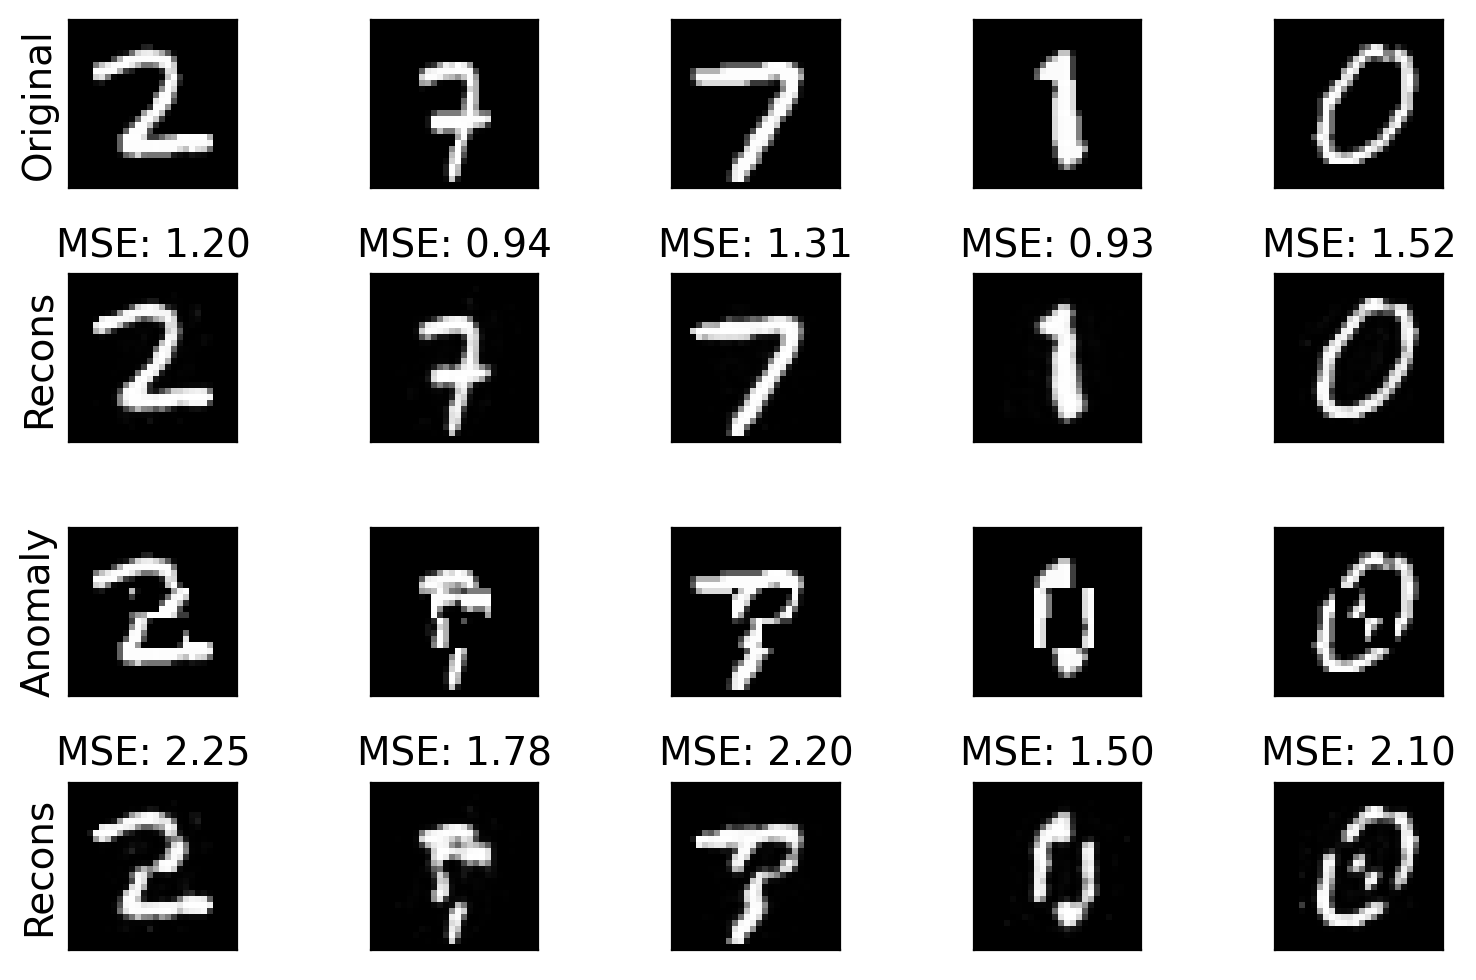
\includegraphics[width=0.5\textwidth]{figures/anomalyimgs.png}
        \end{figure}
    }
    \only<4>{
        \begin{figure}
            \centering
            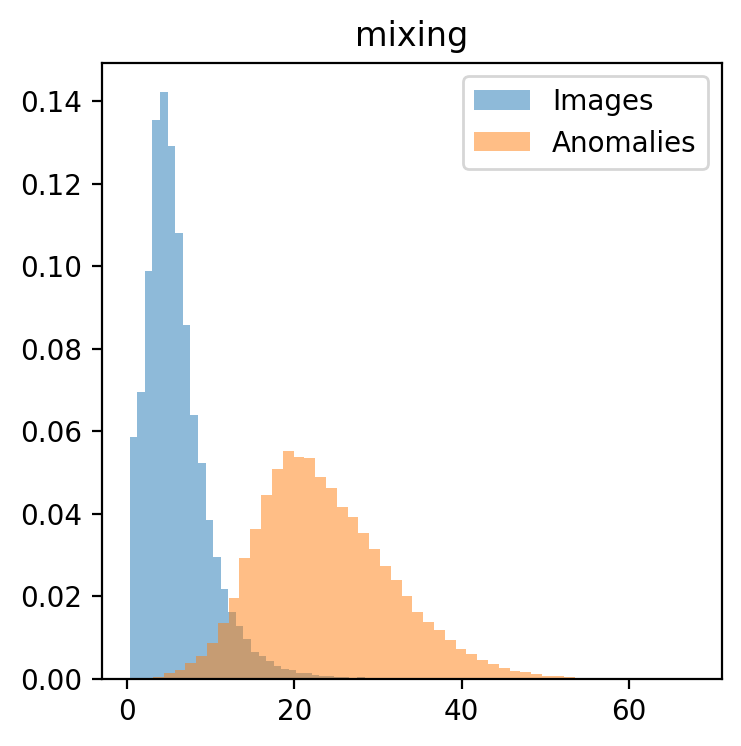
\includegraphics[width=0.35\textwidth]{figures/anoimaly.png}
        \end{figure}
    }
    \only<2>{
        \begin{figure}
            \centering
            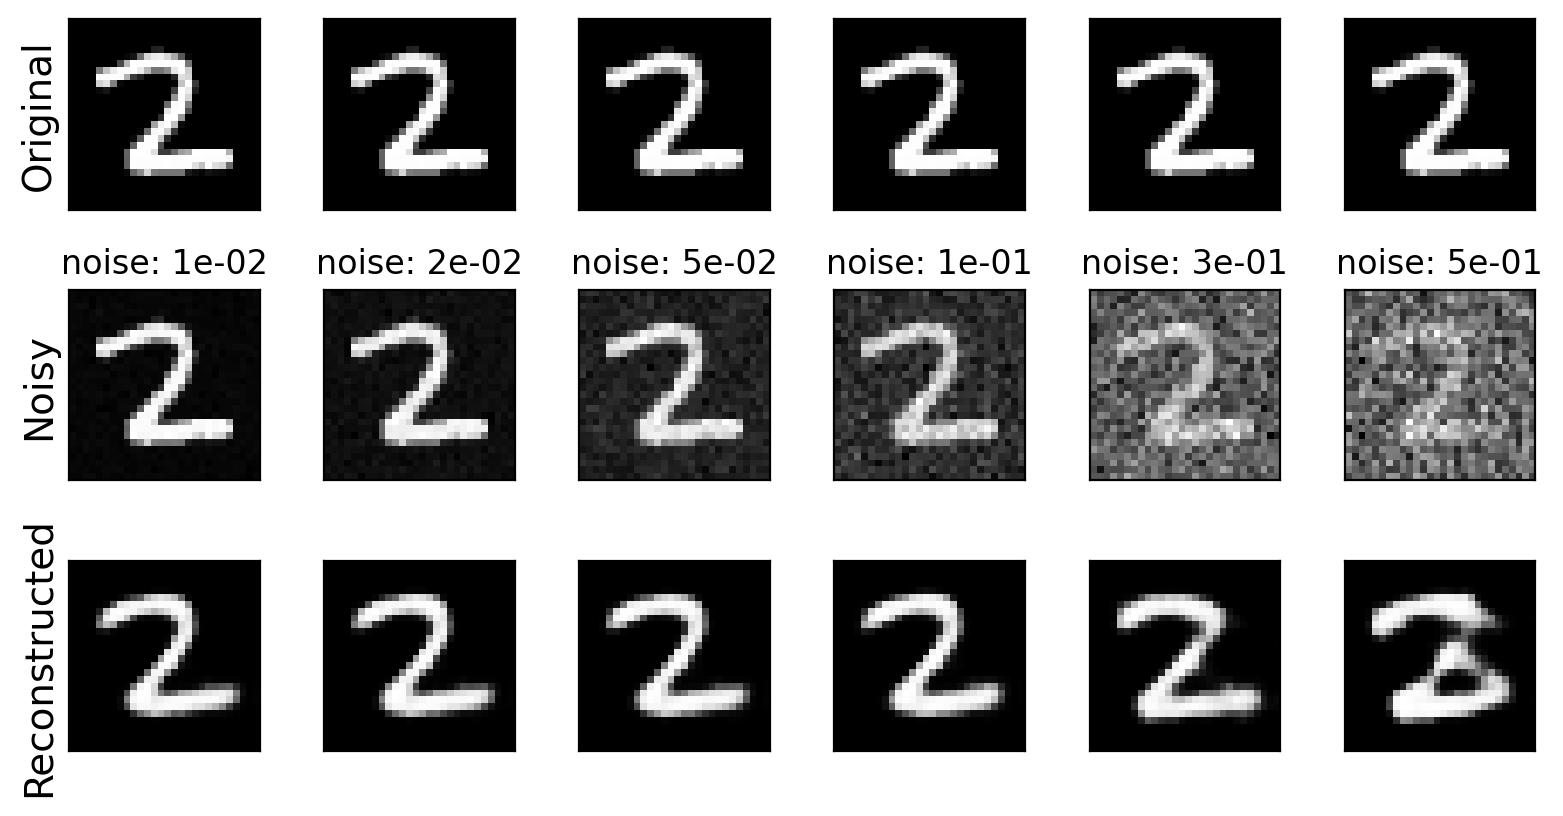
\includegraphics[width=0.6\textwidth]{figures/denoise.png}
        \end{figure}
    }
\end{frame}

\begin{frame}{}{Your turn ! }
    Get the Notebook on the course website and start working on it.
    \begin{itemize}
        \item \url{https://www.alexverine.com}
        \item Teaching
        \item Introduction to Deep Learning
        \item Lien Notebook
    \end{itemize}


\end{frame}



\section{Image Segmentation with U-Net: Correctly evaluate the model}

\subsection{Image Segmentation}

\begin{frame}
    Image segmentation is the process of partitioning an image into multiple segments or regions based on the characteristics of the pixels. It is a fundamental task in computer vision and has applications in various fields, including medical imaging, autonomous driving, and satellite image analysis. There are several methods for image segmentation, including thresholding, clustering, and deep learning-based approaches. In this section, we will focus on a deep learning model called U-Net, which is commonly used for image segmentation tasks.

    \begin{figure}
        \centering
        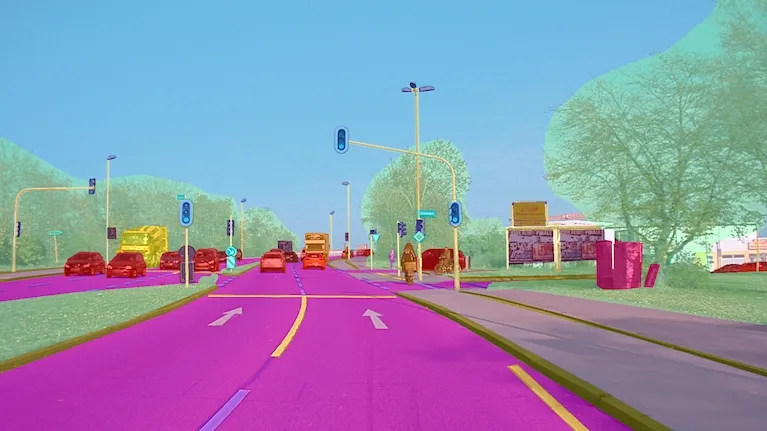
\includegraphics[width = 0.6\textwidth]{figures/imageseg.png}
    \end{figure}
\end{frame}

\begin{frame}{}{Applications of Image Segmentation}
    Image segmentation has a wide range of applications in computer vision and image processing, including:
    \begin{itemize}
        \item Medical Imaging: Segmentation of organs, tumors, and other structures in medical images.
        \item Autonomous Driving: Segmentation of objects such as cars, pedestrians, and road signs in images captured by autonomous vehicles.
        \item Satellite Image Analysis: Segmentation of land cover types, buildings, and other features in satellite images.
        \item Object Detection: Segmentation of objects in images to localize and classify them.
        \item Image Editing: Segmentation of objects for image editing tasks such as background removal and image compositing.
    \end{itemize}
\end{frame}

\begin{frame}{}{Type of Segmentations}
    \begin{minipage}[t]{0.48\textwidth}

        Image segmentation can be broadly classified into two types: semantic segmentation and instance segmentation.
        \begin{itemize}
            \item \textbf{Semantic Segmentation:} Semantic segmentation assigns a class label to each pixel in an image, such as road, car, person, etc. The goal is to partition the image into semantically meaningful regions.
            \item \textbf{Instance Segmentation:} Instance segmentation goes a step further than semantic segmentation by distinguishing between different instances of the same class. It assigns a unique label to each object instance in the image.
        \end{itemize}
    \end{minipage}
    \hfill
    \begin{minipage}[t]{0.48\textwidth}
        \begin{figure}
            \centering
            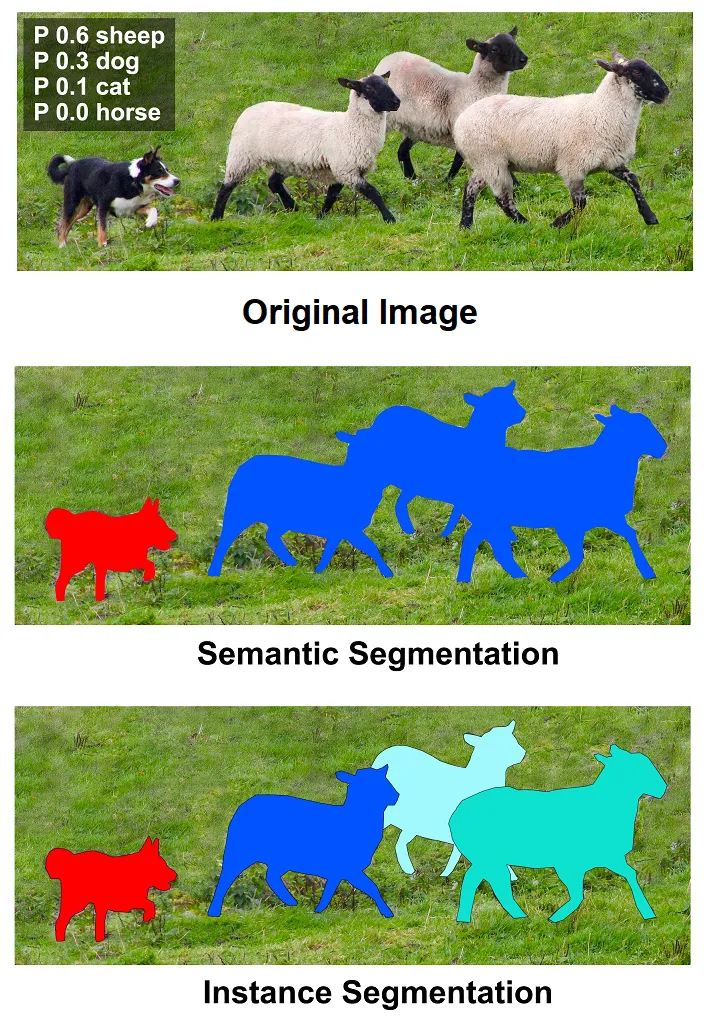
\includegraphics[width = 0.6\textwidth]{figures/typeseg.png}
        \end{figure}
    \end{minipage}
\end{frame}


\subsection{Image Segmentation with U-Net}
\begin{frame}
    U-Net is a convolutional neural network architecture designed for image segmentation tasks. It consists of an encoder-decoder structure with skip connections that allow the model to capture both local and global features in the input image.
    \vfill
    \begin{figure}
        \centering
        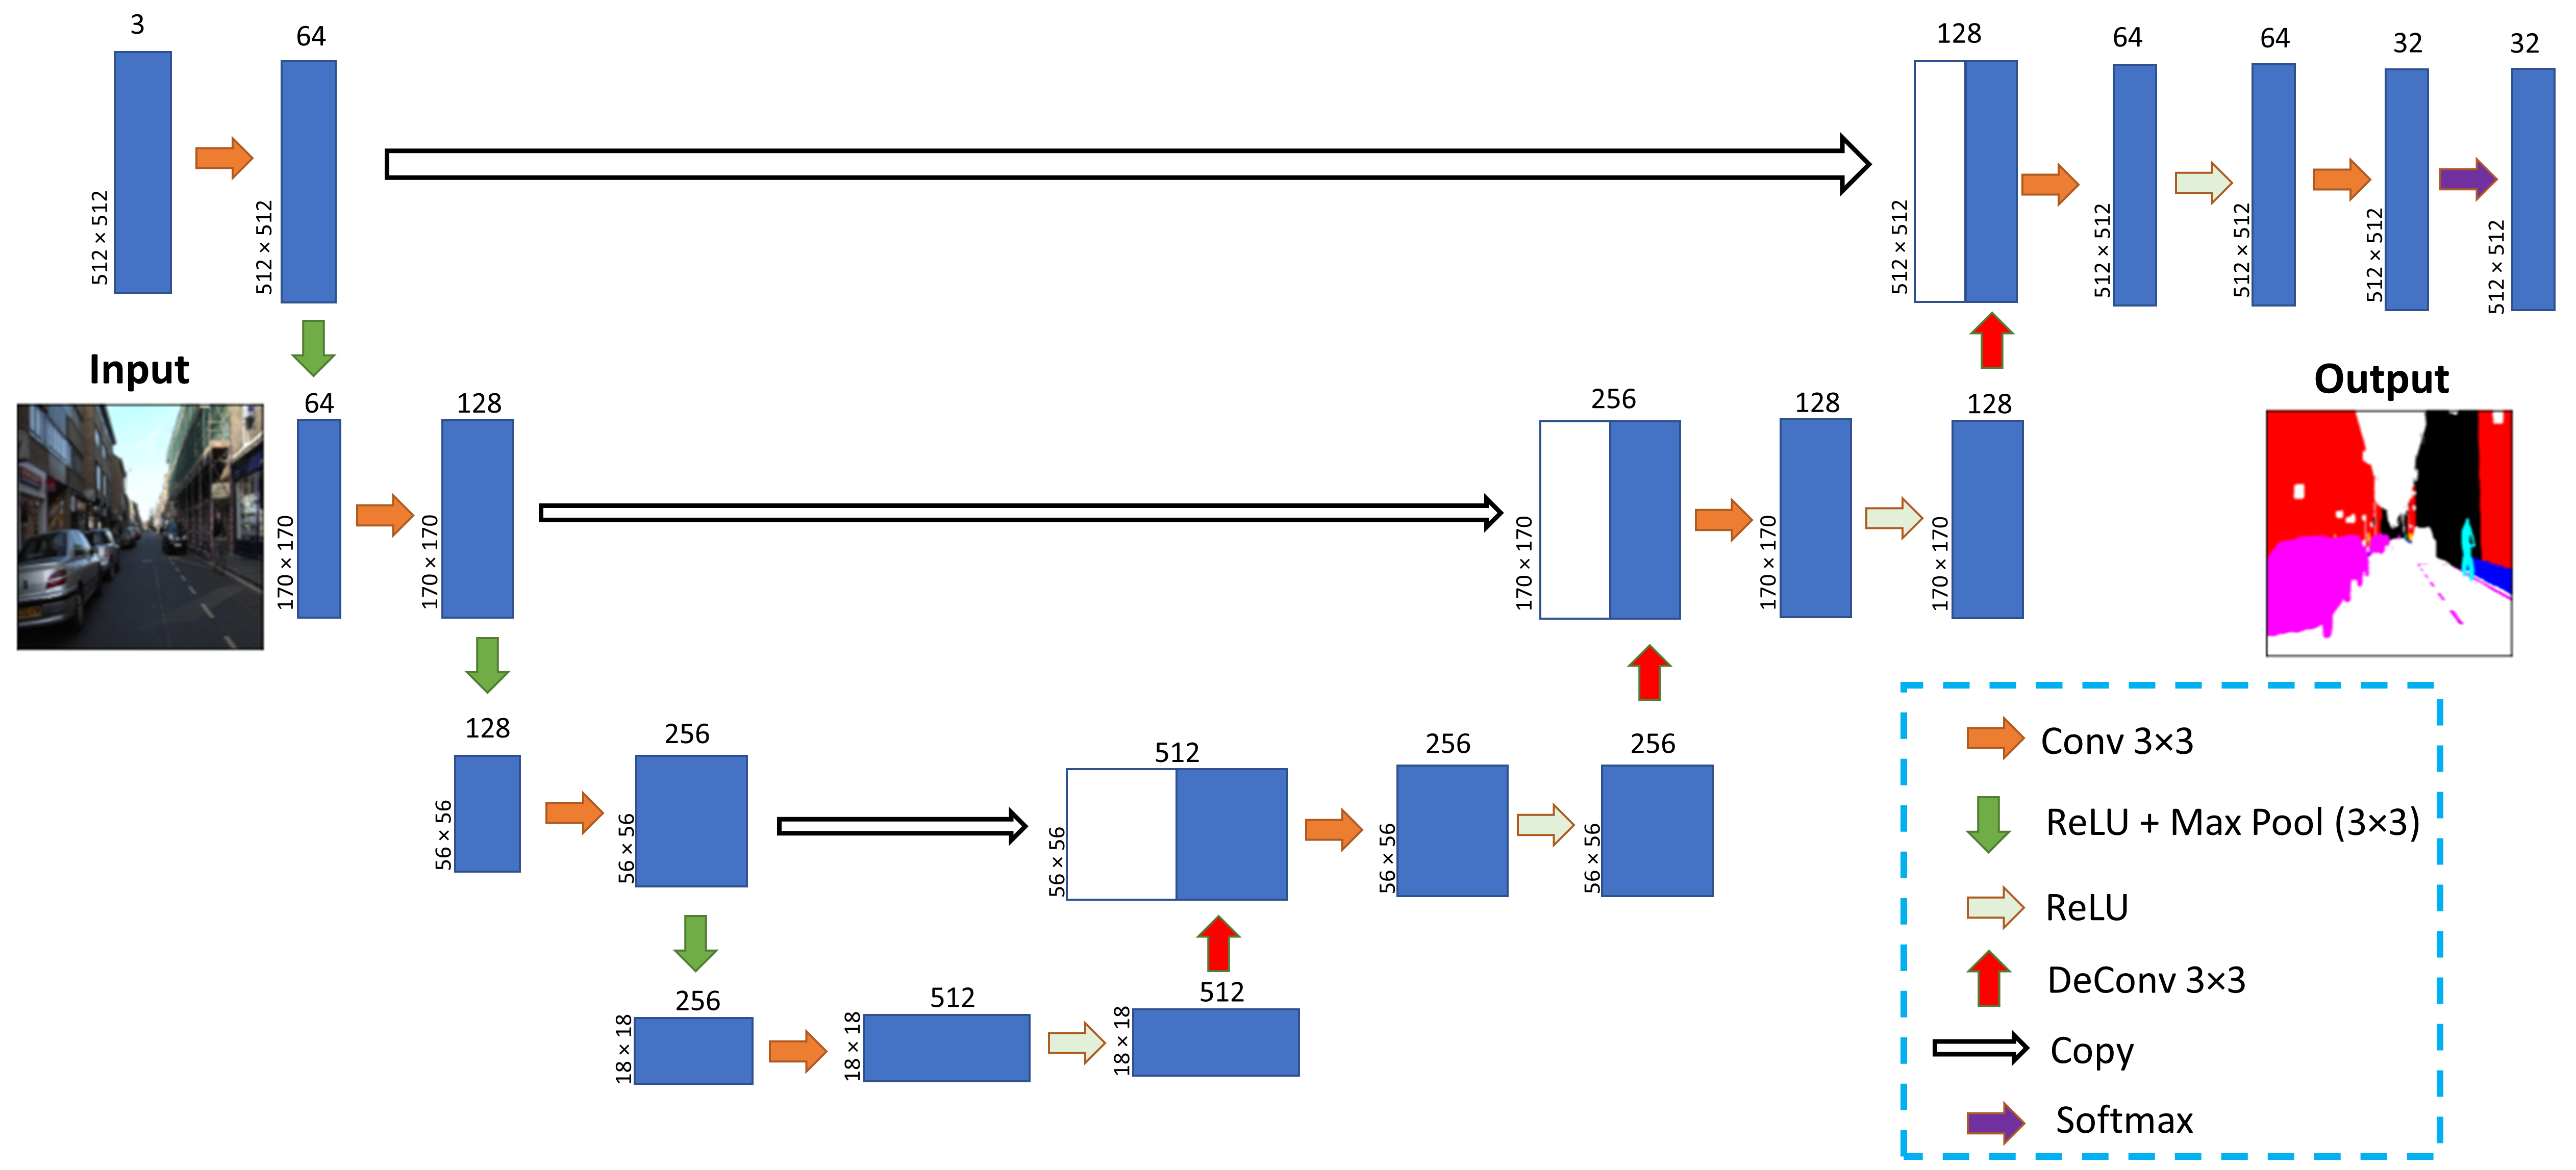
\includegraphics[width = 1\textwidth]{figures/U_Net_arch.png}
    \end{figure}
\end{frame}

\begin{frame}{}{Loss Functions}
    3 main loss functions are used for image segmentation tasks:
    \begin{itemize}
        \item \textbf{Categorical Cross-Entropy Loss:} Used for multi-class segmentation tasks where each pixel is classified into one of multiple classes.
              \only<2>{
              $$\mathcal{L} = -\frac{1}{N}\sum_{i=1}^{N}\sum_{c=1}^{C}y_{i,c}\log(\hat{y}_{i,c})$$
              }
        \item \textbf{Dice Loss:} A similarity-based loss function that measures the overlap between the predicted segmentation mask and the ground truth mask.
              \only<3>{
                  $$\mathcal{L} = 1 - \frac{2\sum_{i=1}^{N}y_i\hat{y}_i}{\sum_{i=1}^{N}y_i + \sum_{i=1}^{N}\hat{y}_i}$$
              }
        \item \textbf{Shaped aware Loss:} A loss function that penalizes the model for making errors near the object boundaries, where the segmentation is most critical.
              \only<4>{
              $$\mathcal{L} = -w(x)\left[\frac{1}{N}\sum_{i=1}^{N}\sum_{c=1}^{C}y_{i,c}\log(\hat{y}_{i,c})\right]$$
              with $w(x)$ a weight function that assigns higher weights to pixels near the object boundaries.
              }
    \end{itemize}
\end{frame}


\begin{frame}{}{The dataset}
    The dataset presented here is hosted in the BioStudies database under accession number S-BSST265 18. It consists of 79 fluorescence images of immuno and DAPI stained samples containing 7813 nuclei in total. The images are derived from one Schwann cell stroma-rich tissue (from a ganglioneuroblastoma) cryosection (10 images/2773 nuclei), seven neuroblastoma (NB) patients (19 images/931 nuclei), one Wilms patient (1 image/102 nuclei), two NB cell lines (CLB-Ma, STA-NB10) (8 images/1785 nuclei) and a human keratinocyte cell line (HaCaT) (41 images/2222 nuclei). In addition, the dataset is heterogenous in aspects such as type of preparation, imaging modality, magnification, signal-to-noise ratio and other technical aspects.
    \begin{figure}
        \centering
        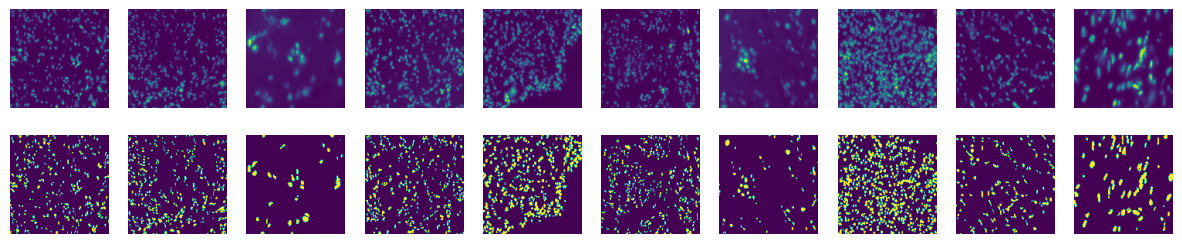
\includegraphics[width=0.8\textwidth]{figures/imagesegbio.png}
    \end{figure}
\end{frame}

% \begin{frame}{}{The U-Net Architecture}
%     U-Net is a convolutional neural network architecture designed for encoding/decoding images. It is widely used for image segmentation tasks:
%     \begin{figure}
%         \centering
%         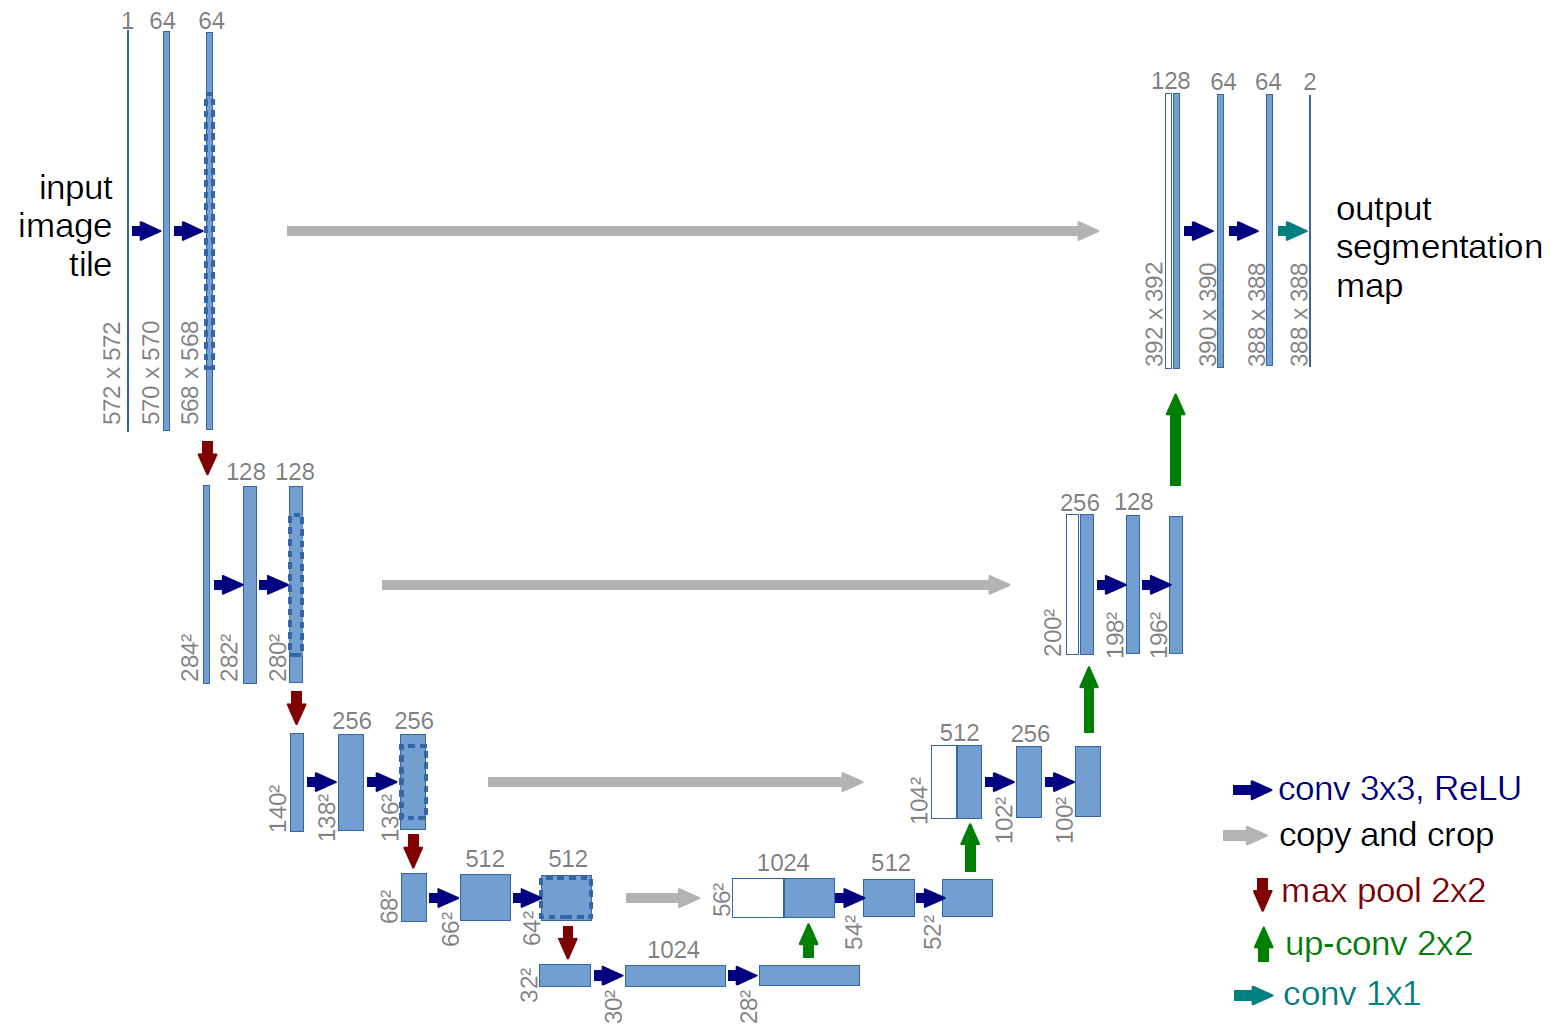
\includegraphics[width=0.7\textwidth]{figures/u-net-architecture.png}
%     \end{figure}
% \end{frame}


\subsection{Evaluating the models}

\begin{frame}
    In this example, the model is trained with the Binary Cross-Entropy loss function. Each pixel $y_{i,j}$is a label in $\{0, 1\}$, where $0$ represents the background and $1$ represents the object. The loss function is defined as:
    \[
        \text{BCE}(y, \hat{y}) = -\frac{1}{N^2} \sum_{i=1}^{N}\sum_{j=1}^{N} y_{i,j} \log(\hat{y}_{i,j}) + (1 - y_{i,j}) \log(1 - \hat{y}_{i,j})
    \]
    where $N$ is the number of pixels in the image, $y$ is the ground truth mask, and $\hat{y}$ is the predicted mask. The BCE loss function is used to measure the pixel-wise binary classification error between the ground truth and the predicted mask.
    \vspace{0.5cm}
    \textbf{Question:} What can we use to evaluate the performance of the model?
\end{frame}

\begin{frame}{}{Interpreting the output}
    The first metrics that comes to mind is cross-entropy on the test set. However, it is not the best metric to evaluate the performance of a segmentation model. The reason is that the model predicts probabilities for each pixel, and the thresholding of these probabilities is not taken into account in the BCE loss.\\
    \vspace{1cm}
    The model predicts values in $\mathbb{R}$ for each pixel. We can use a threshold to binarize the predictions:
    \vfill
    \begin{figure}
        \centering
        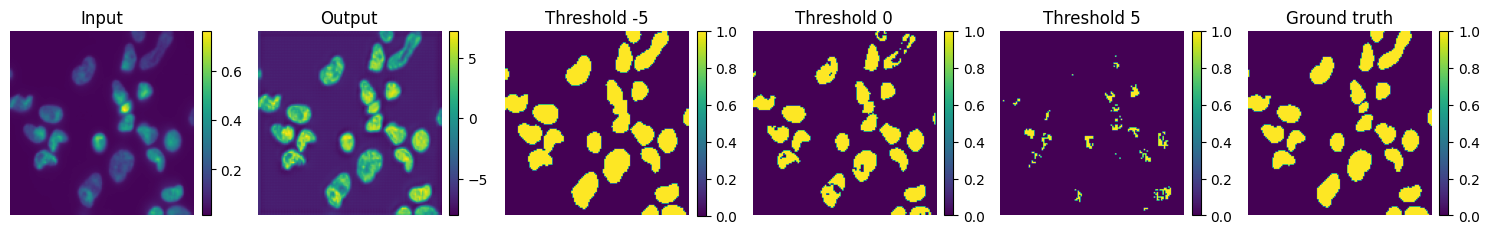
\includegraphics[width=1\textwidth]{figures/outputs.png}
    \end{figure}

\end{frame}

\begin{frame}[t]{}{The Accuracy}
    The accuracy is a common metric used to evaluate the performance of classification models. The accuracy is defined as:
    \[
        \text{Accuracy} = \frac{\text{Number of correct predictions}}{\text{Total number of predictions}}
    \]
    \vfill
    \begin{figure}
        \centering
        \only<1>{
            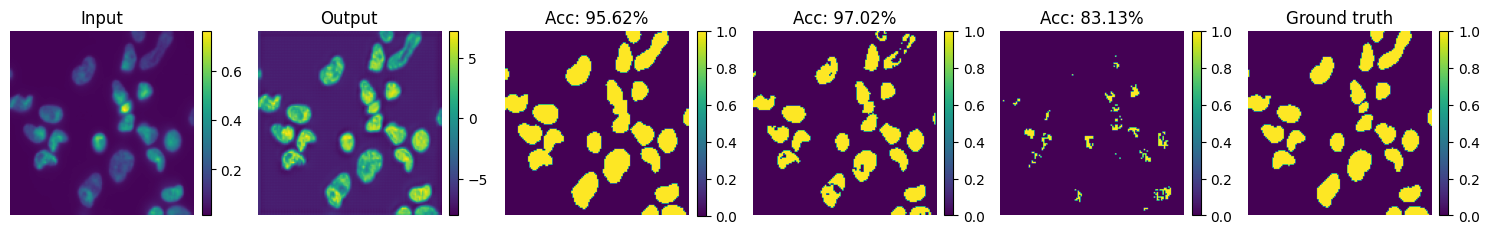
\includegraphics[width=0.9\textwidth]{figures/accs.png}}
        \only<2>{
            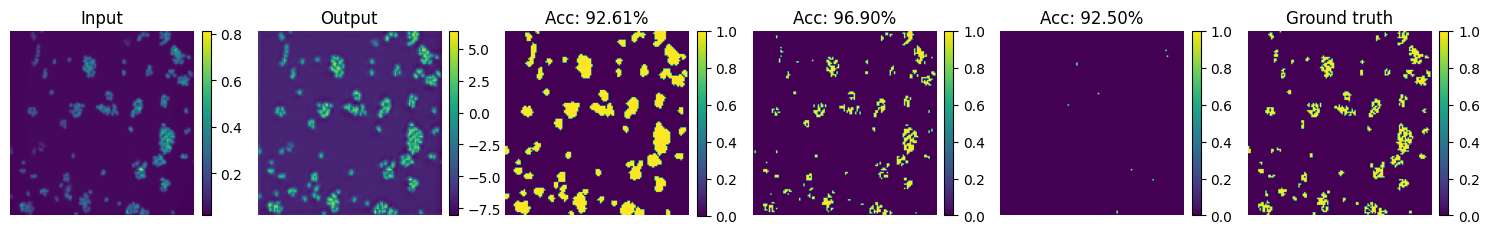
\includegraphics[width=0.9\textwidth]{figures/accs2.png}}
    \end{figure}
    \only<2>{However, missing a label $0$ is not the same as missing a label $1$ ! }
\end{frame}

\begin{frame}{}{Confusion Matrix}
    The confusion matrix is a useful tool for evaluating classification models, particularly for segmentation. It helps to distinguish between different types of errors.

    \vfill
    \begin{columns}
        \column{0.4\textwidth}
        \begin{itemize}
            \item \textbf{True Positives (TP)}: \\Correctly predicted positives.
            \item \textbf{False Positives (FP)}: \\Incorrectly predicted positives.
            \item \textbf{False Negatives (FN)}: \\Missed positives.
            \item \textbf{True Negatives (TN)}: \\Correctly predicted negatives.
        \end{itemize}

        \column{0.6\textwidth}
        \centering
        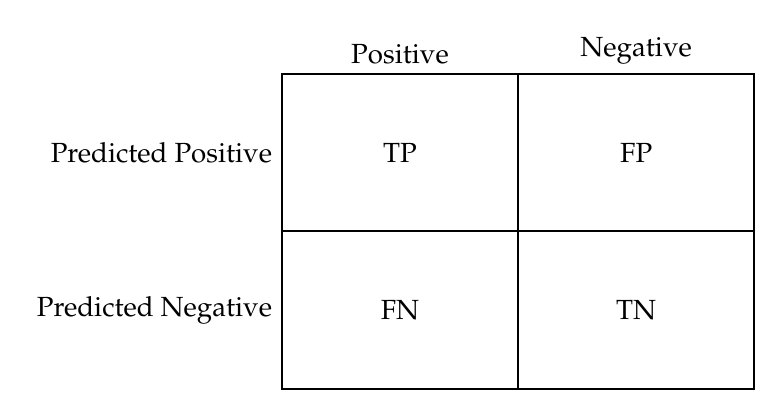
\begin{tikzpicture}
            \draw[thick] (0,0) rectangle (6,4);

            % Grid lines
            \draw[thick] (3,0) -- (3,4);
            \draw[thick] (0,2) -- (6,2);

            % Labels
            \node[anchor=south] at (1.5,4) {Positive};
            \node[anchor=south] at (4.5,4) {Negative};
            \node[anchor=east] at (0,3) {Predicted Positive};
            \node[anchor=east] at (0,1) {Predicted Negative};

            % Matrix Entries
            \node at (1.5,3) {TP};
            \node at (4.5,3) {FP};
            \node at (1.5,1) {FN};
            \node at (4.5,1) {TN};
        \end{tikzpicture}
    \end{columns}
\end{frame}

\begin{frame}{}{Precision and Recall}
    \begin{columns}

        \column{0.6\textwidth}
        \centering
        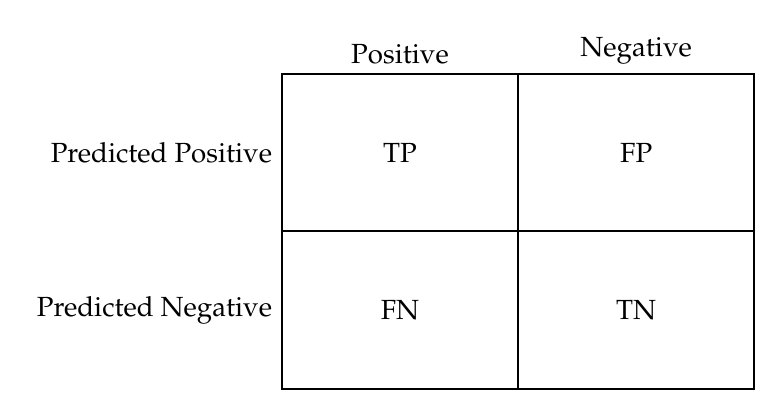
\begin{tikzpicture}
            \draw[thick] (0,0) rectangle (6,4);

            % Grid lines
            \draw[thick] (3,0) -- (3,4);
            \draw[thick] (0,2) -- (6,2);

            % Labels
            \node[anchor=south] at (1.5,4) {Positive};
            \node[anchor=south] at (4.5,4) {Negative};
            \node[anchor=east] at (0,3) {Predicted Positive};
            \node[anchor=east] at (0,1) {Predicted Negative};

            % Matrix Entries
            \node at (1.5,3) {TP};
            \node at (4.5,3) {FP};
            \node at (1.5,1) {FN};
            \node at (4.5,1) {TN};
        \end{tikzpicture}
        \column{0.4\textwidth}
        To evaluate the performance of a segmentation model, we can use the following metrics:
        \begin{align*}
            \mathrm{Accuracy} & = \frac{TP + TN}{P + N}
        \end{align*}
        \begin{align*}
            \mathrm{Precision} & = \frac{TP}{TP + FP}
        \end{align*}
        \begin{align*}
            \mathrm{Recall} & = \frac{TP}{P}
        \end{align*}
    \end{columns}

\end{frame}

\begin{frame}{}{Confusion Matrix}
    Examples with a cancer detection model with 100 patients (20 with cancer and 80 without cancer):
    \begin{center}
        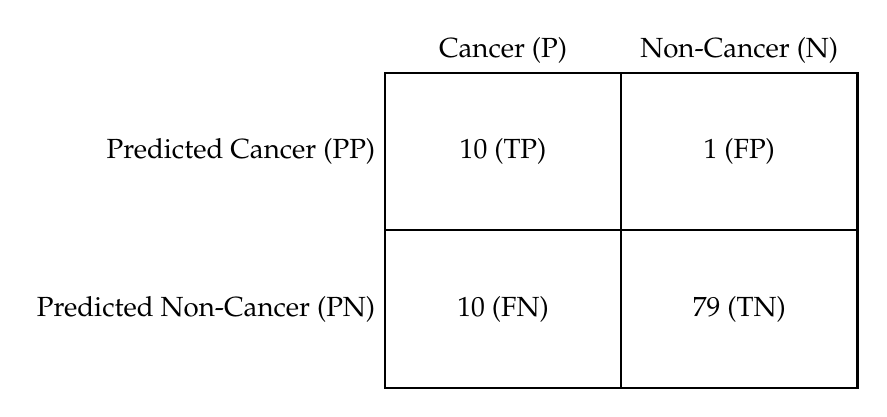
\begin{tikzpicture}
            \draw[thick] (0,0) rectangle (6,4);

            % Grid lines
            \draw[thick] (3,0) -- (3,4);
            \draw[thick] (0,2) -- (6,2);

            % Labels
            \node[anchor=south] at (1.5,4) {Cancer (P)};
            \node[anchor=south] at (4.5,4) {Non-Cancer (N)};
            \node[anchor=east] at (0,3) {Predicted Cancer (PP)};
            \node[anchor=east] at (0,1) {Predicted Non-Cancer (PN)};

            % Matrix Entries
            \node at (1.5,3) {10 (TP)};
            \node at (4.5,3) {1 (FP)};
            \node at (1.5,1) {10 (FN)};
            \node at (4.5,1) {79 (TN)};
        \end{tikzpicture}
        \\
        \vspace{1cm}
        Accuracy: $\frac{TP + TN}{P + N} = \frac{10 + 79}{20 + 80} = 0.89\quad$  Precision: $\frac{TP}{TP + FP} = \frac{10}{10 + 1} = 0.90\quad$ Recall: $\frac{TP}{P} = \frac{10}{20} = 0.5$
    \end{center}
\end{frame}

\begin{frame}{}{Confusion Matrix}
    Examples with a financial operation models with 100 operations (20 high reward and 80 high loss):
    \begin{center}
        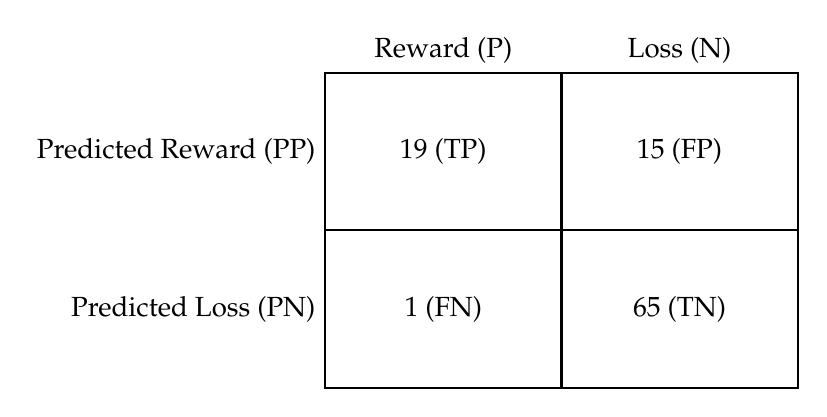
\begin{tikzpicture}
            \draw[thick] (0,0) rectangle (6,4);

            % Grid lines
            \draw[thick] (3,0) -- (3,4);
            \draw[thick] (0,2) -- (6,2);

            % Labels
            \node[anchor=south] at (1.5,4) {Reward (P)};
            \node[anchor=south] at (4.5,4) {Loss (N)};
            \node[anchor=east] at (0,3) {Predicted Reward (PP)};
            \node[anchor=east] at (0,1) {Predicted Loss (PN)};

            % Matrix Entries
            \node at (1.5,3) {19 (TP)};
            \node at (4.5,3) {15 (FP)};
            \node at (1.5,1) {1 (FN)};
            \node at (4.5,1) {65 (TN)};
        \end{tikzpicture}
        \\
        \vspace{1cm}
        Accuracy: $\frac{TP + TN}{P + N} = \frac{19 + 65}{20 + 80} = 0.84\quad$  Precision: $\frac{TP}{TP + FP} = \frac{19}{19 + 15} = 0.56\quad$ Recall: $\frac{TP}{P} = \frac{19}{20} = 0.95$
    \end{center}
\end{frame}


\begin{frame}{}{Precision-Recall Curve}
    In Image segmentation tasks, by adjusting the threshold we can change the precision and recall of the model. The Precision-Recall curve is a useful tool to evaluate the performance of a model across different thresholds:
    \begin{figure}
        \centering
        \only<1>{
            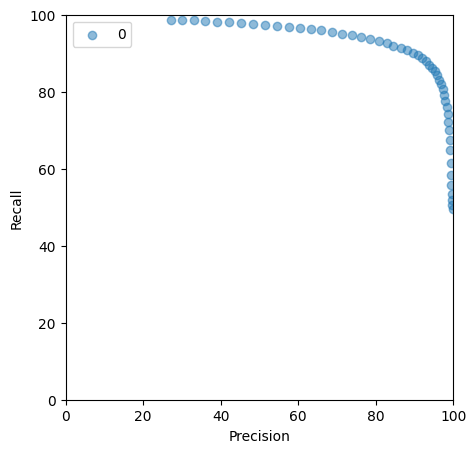
\includegraphics[width=0.5\textwidth]{figures/prcurve.png}}
        \only<2>{
            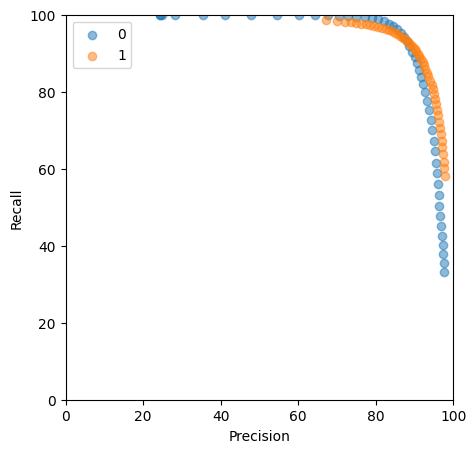
\includegraphics[width=0.5\textwidth]{figures/prcurve2.png}}
    \end{figure}
\end{frame}

\begin{frame}{}{Your turn !}
    Get the Notebook on the course website and start working on it.
    \begin{itemize}
        \item \url{https://www.alexverine.com}
        \item Teaching
        \item Introduction to Deep Learning
        \item Lien Notebook
    \end{itemize}
    During this hands-on session we will compare the speed of the model with and without the GPU, and we will evaluate the model with the metrics we have seen. Don't hesitate to use Colab or your own computer to run the notebook.
\end{frame}



\section{Synthetic Data Generation with Generative Adversarial Networks}
\subsection{GANS Models}
\begin{frame}
    Generative Adversarial Networks (GANs) are a type of deep learning architecture composed of two neural networks, the generator and the discriminator, that are trained in a adversarial manner. The generator network is trained to generate fake data that appears similar to real data, while the discriminator network is trained to distinguish between real and fake data. The loss for GANs is defined as a min-max game, where the generator minimizes the loss function, and the discriminator maximizes it. $D$ and $G$ represent the discriminator and generator networks, respectively, and the goal is to find the optimal configuration for $D$ and $G$ such that the generated samples appear indistinguishable from real data.

    \begin{figure}
        \centering
        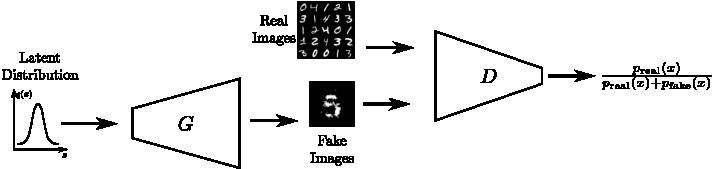
\includegraphics[width = 0.9\textwidth]{figures/GAN.pdf}
    \end{figure}
\end{frame}
\begin{frame}
    The loss of a  (GAN) is defined as a minimax game between the generator and discriminator models. The generator aims to generate samples that are indistinguishable from real samples, while the discriminator aims to distinguish the generated samples from real samples. The loss function for the generator is defined as $-\log(D(G(z)))$, where $D$ is the discriminator model and $G(z)$ is the generator's output for a random noise vector $z$. The loss function for the discriminator is defined as $\log(D(x)) + \log(1 - D(G(z)))$, where $x$ is a real sample.
    $$
        \min_D \max_G \mathbb{E}_{x\sim p_{\mathrm{real}}}\left[\log(D(x))\right]  +  \mathbb{E}_{z\sim q}\left[ \log(1 - D(G(z)))\right]
    $$

    \begin{figure}
        \centering
        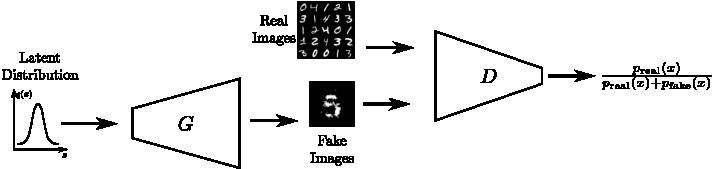
\includegraphics[width = 0.9\textwidth]{figures/GAN.pdf}
    \end{figure}
\end{frame}

% --- SLIDE 1 ---
\begin{frame}{Generative Adversarial Networks (GANs)}{Intro: year, reference, roles of D \& G}
    \textbf{Introduced in:} 2014a by \citet{goodfellow_generative_2014}.\\
    \medskip
    \begin{itemize}
        \item \textbf{Discriminator $D(x)$}: estimates how likely a sample $x$ is \emph{real} (vs. generated).
        \item \textbf{Generator $G(z)$}: maps noise $z\sim Q$ to data space and aims to \emph{fool} $D$.
    \end{itemize}
    \begin{figure}
        \centering
        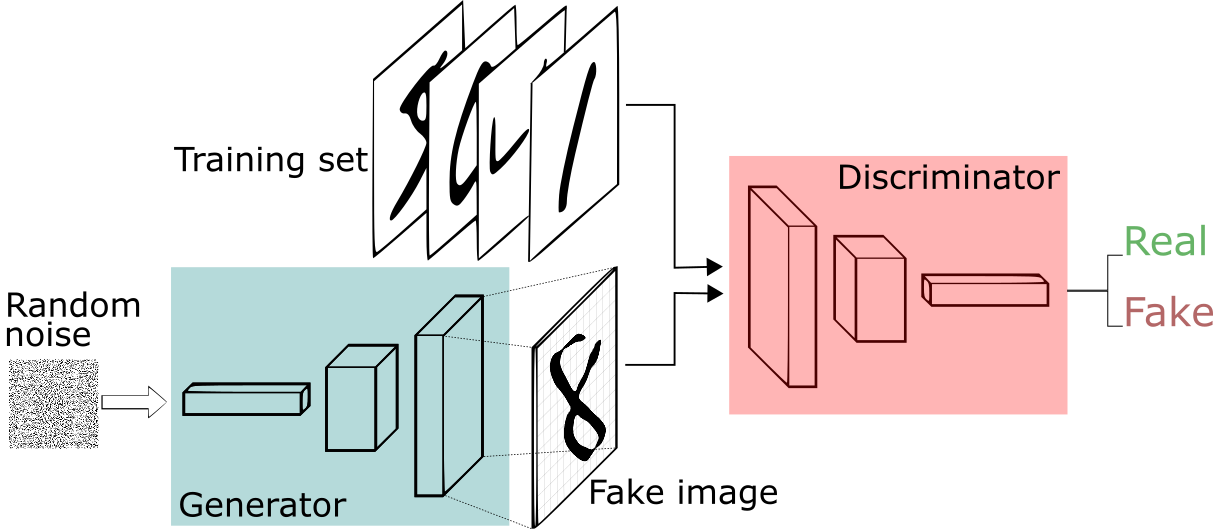
\includegraphics[width=0.8\textwidth]{figures/GANs.png}
    \end{figure}
\end{frame}

% --- SLIDE 1.5.1 ---
\begin{frame}[t]{Training the Discriminator as a Classifier}{Labels, loss selection, BCE/logistic}
    \only<1->{
        \textbf{Setup:} assign labels $y\in\{-1, +1\}$ with $y=+1$ for real $x\sim P$ and $y=-1$ for fake $x\sim \widehat{P}$.\\
        \textbf{Goal:} Train a classifier parametrized by $D=\sigma(F_\theta)$ to distinguish real vs fake.\\
        \medskip
        \textbf{Question:} which loss to train $D$ as a classifier?
    }

\end{frame}

% Replace frame title and subtitle as requested
\begin{frame}{Sigmoid and Logit}{Activation \& link functions}
    \begin{itemize}
        \item The \textbf{sigmoid function} $\sigma:\mathbb{R}\to[0,1]$ is defined as:
              \begin{equation}
                  \sigma(x) = \frac{1}{1+\exp(-x)}.
              \end{equation}
        \item It maps any real-valued number $x$ to the interval $[0,1]$, suitable for modeling probabilities.
        \item The \textbf{logit function} $\text{logit}:[0,1]\to\mathbb{R}$ is defined as the inverse of the sigmoid:
              \begin{equation}
                  \text{logit}(p) = \log\left(\frac{p}{1-p}\right).
              \end{equation}
        \item Let $D(x) = \sigma(F_\theta(x))$ be a discriminator outputting probabilities. We call $F_\theta(x)$ the \textbf{logit} of $D$ and $D(x)$ the \textbf{probit}.
    \end{itemize}
    \medskip
    \begin{figure}
        \centering
        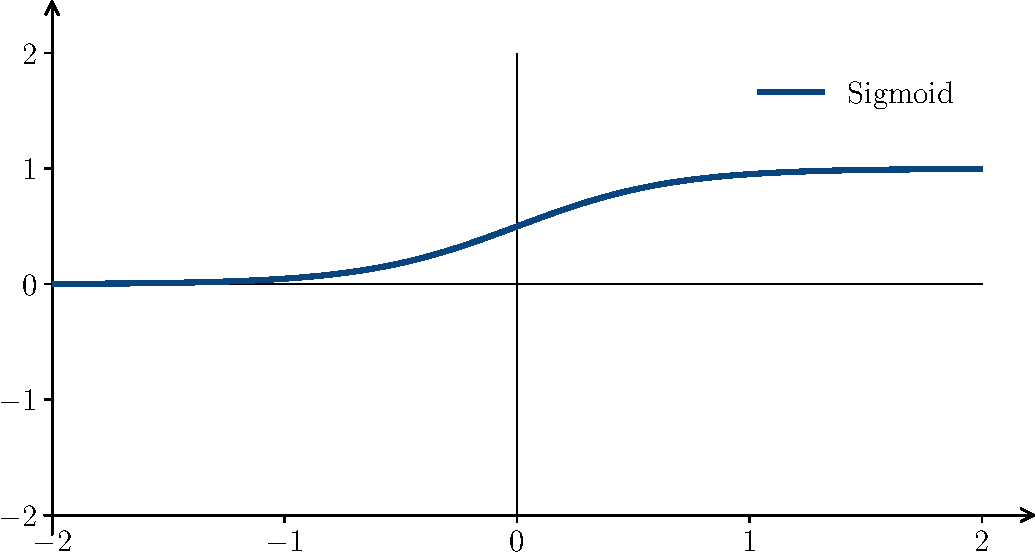
\includegraphics[width=0.35\textwidth]{figures/sigmoid.pdf}
        \caption{Sigmoid function mapping logits to probabilities.}
    \end{figure}
\end{frame}


% --- SLIDE 1.5.1 ---
\begin{frame}[t]{Training the Discriminator as a Classifier}{Question → Answer → Loss decomposition}
    \only<1->{
        \textbf{Setup:} assign labels $y\in\{-1, +1\}$ with $y=+1$ for real $x\sim P$ and $y=-1$ for fake $x\sim \widehat{P}$.\\
        \textbf{Goal:} Train a classifier parametrized by $D=\sigma(F_\theta)$ to distinguish real vs fake.\\
        \medskip
        \only<1>{
            \textbf{Question:} which loss to train $D$ as a classifier?}
    }
    \only<2->{
        \textbf{Answer:} binary cross-entropy / logistic loss (with logits).\\
    }
    \only<3->{
        \textbf{Loss with labels:}
        \begin{equation*}
            \mathcal{L}_D = \mathbb{E}_{(x,y)}\Big[\log\big(1+\exp(-y\, F_\theta(x))\big)\Big].
        \end{equation*}
        \textbf{Decomposition over $P$ and $\widehat{P}$:}
        \begin{align*}
            \mathcal{L}_D & = \mathbb{E}_{x\sim P}\big[\log(1+\exp(-F_\theta(x)))\big]
            \quad + \mathbb{E}_{x\sim \widehat{P}}\big[\log(1+\exp(F_\theta(x)))\big]                                                                                                                          \\
                          & =\mathbb{E}_{x\sim P}\big[- \log \left(\frac{1}{1+\exp(-F_\theta(x))}\right)\big] + \mathbb{E}_{x\sim \widehat{P}}\big[- \log \left(1 - \frac{1}{1+\exp(-F_\theta(x))}\right)\big] \\
                          & = -\mathbb{E}_{x\sim P}[\log \sigma(F_\theta(x))] - \mathbb{E}_{x\sim \widehat{P}}[\log(1-\sigma(F_\theta(x)))]                                                                    \\
                          & = -\mathbb{E}_{x\sim P}[\log D(x)] - \mathbb{E}_{x\sim \widehat{P}}[\log(1-D(x))].
        \end{align*}
        \only<4>{
            Summarizing:
            \begin{equation*}
                \boxed{\text{Minimizing }\mathcal{L}_D = -\mathbb{E}_{x\sim P}[\log D(x)] - \mathbb{E}_{x\sim \widehat{P}}[\log(1-D(x))].}
            \end{equation*}}
        \only<5>{
            Summarizing:
            \begin{equation*}
                \boxed{\text{Maximizing }\mathcal{L}_D = \mathbb{E}_{x\sim P}[\log D(x)] + \mathbb{E}_{x\sim \widehat{P}}[\log(1-D(x))].}
            \end{equation*}}
    }
\end{frame}


% --- SLIDE 1.5.2 ---
\begin{frame}[t]{Training the Generator}{Minimax vs non-saturating objectives}
    \only<1->{
        \textbf{Goal:} decrease $D$'s confidence on $\widehat{P}$ (make fakes look real).
    }
    \only<2>{
        \begin{equation*}
            \boxed{\text{Maximizing }  \mathcal{L}_G = - \mathbb{E}_{x\sim \widehat{P}}[\log(1-D(x))]}
        \end{equation*}
    }
    \only<3>{
        \begin{equation*}
            \boxed{\text{Maximizing }  \mathcal{L}_G = - \mathbb{E}_{z\sim Q}[\log(1-D(G(z)))]}
        \end{equation*}
    }
    \only<4->{
        \begin{equation*}
            \boxed{\text{Minimizing }  \mathcal{L}_G = \mathbb{E}_{z\sim Q}[\log(1-D((G(z))))]}
        \end{equation*}
    }
    \only<5>{
        \textbf{Minimax formulation:} combine both objectives:
        \begin{equation*}
            \min_G \max_D\ \mathbb{E}_{x\sim P}[\log D(x)] + \mathbb{E}_{z\sim Q}[\log(1-D(G(z)))]
        \end{equation*}
    }
\end{frame}

% --- SLIDE 2 ---
\begin{frame}{Original GAN: Figures}{Training loop \& distributions}
    Example of generated samples during training from \citet{goodfellow_generative_2014}. In dotted black: the real data distribution, in blue the estimated probabilities from the discriminator and in green the generated distribution.
    \vskip 10pt
    \begin{minipage}[t]{0.31\textwidth}
        \begin{figure}
            \centering
            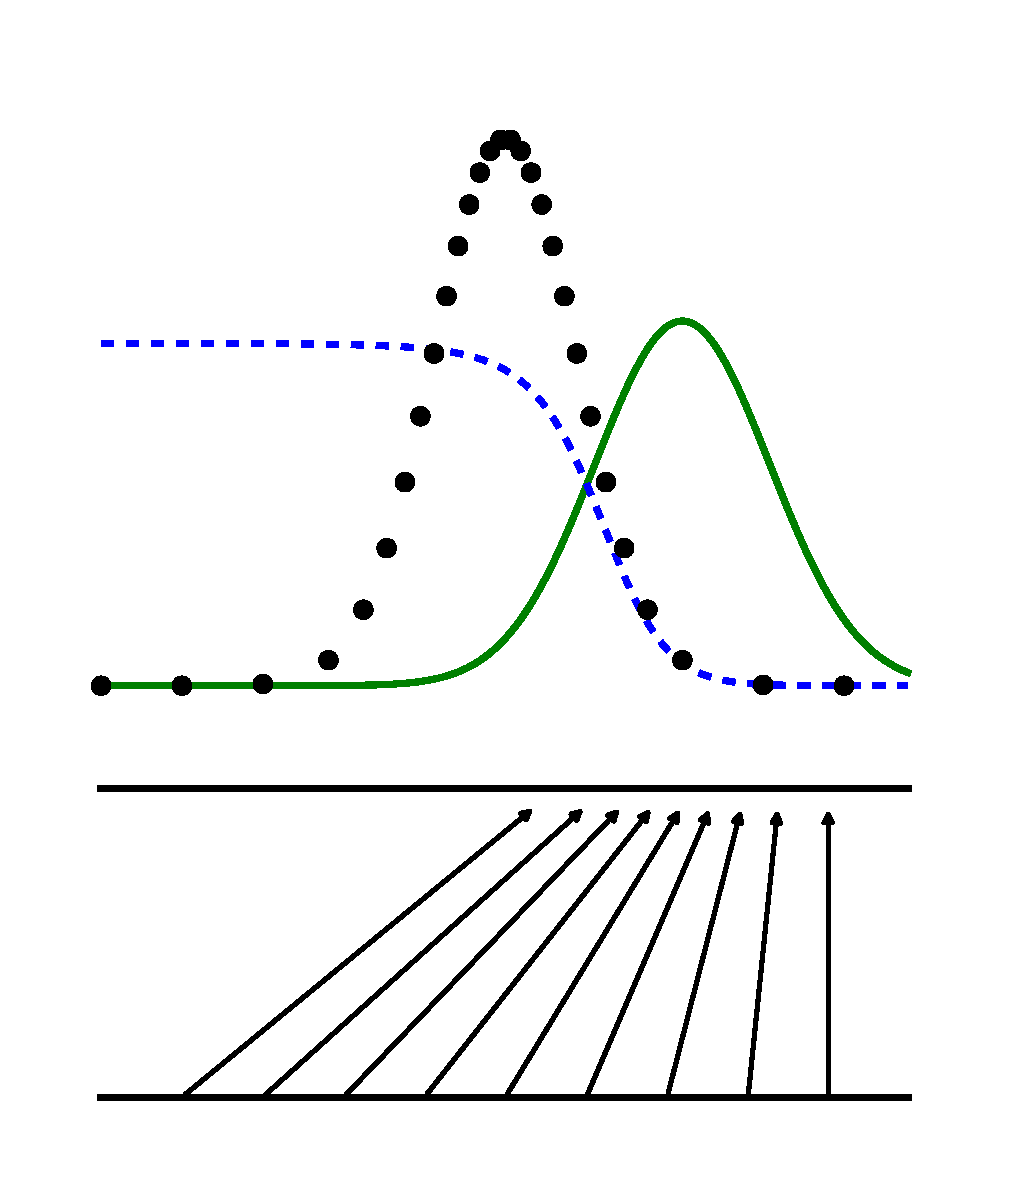
\includegraphics[width=0.9\textwidth]{figures/gan1.pdf}
            \caption{Before}
        \end{figure}
    \end{minipage}
    \hfill
    \begin{minipage}[t]{0.31\textwidth}
        \begin{figure}
            \centering
            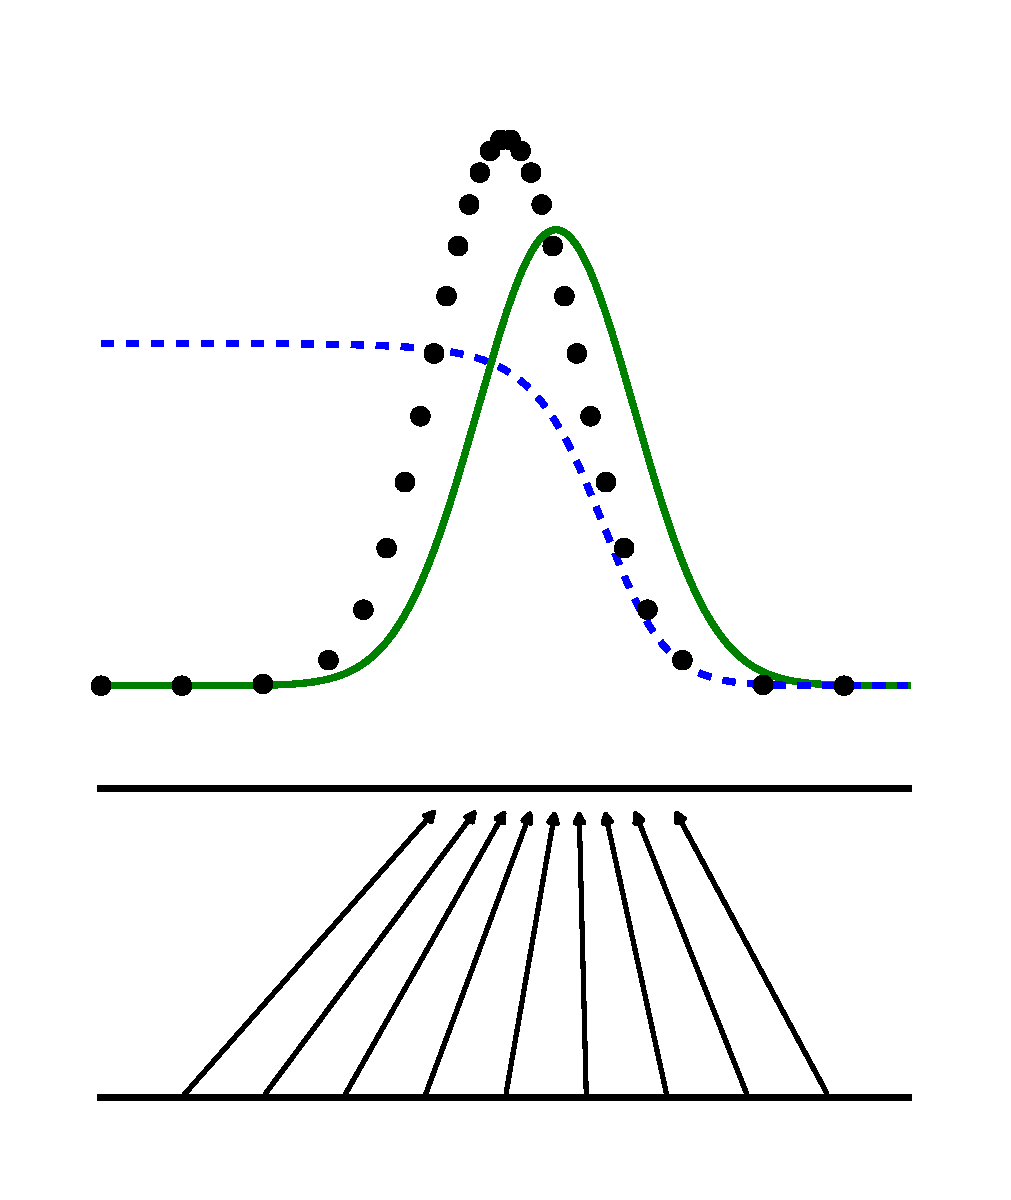
\includegraphics[width=0.9\textwidth]{figures/gan2.pdf}
            \caption{During}
        \end{figure}
    \end{minipage}
    \hfill
    \begin{minipage}[t]{0.31\textwidth}
        \begin{figure}
            \centering
            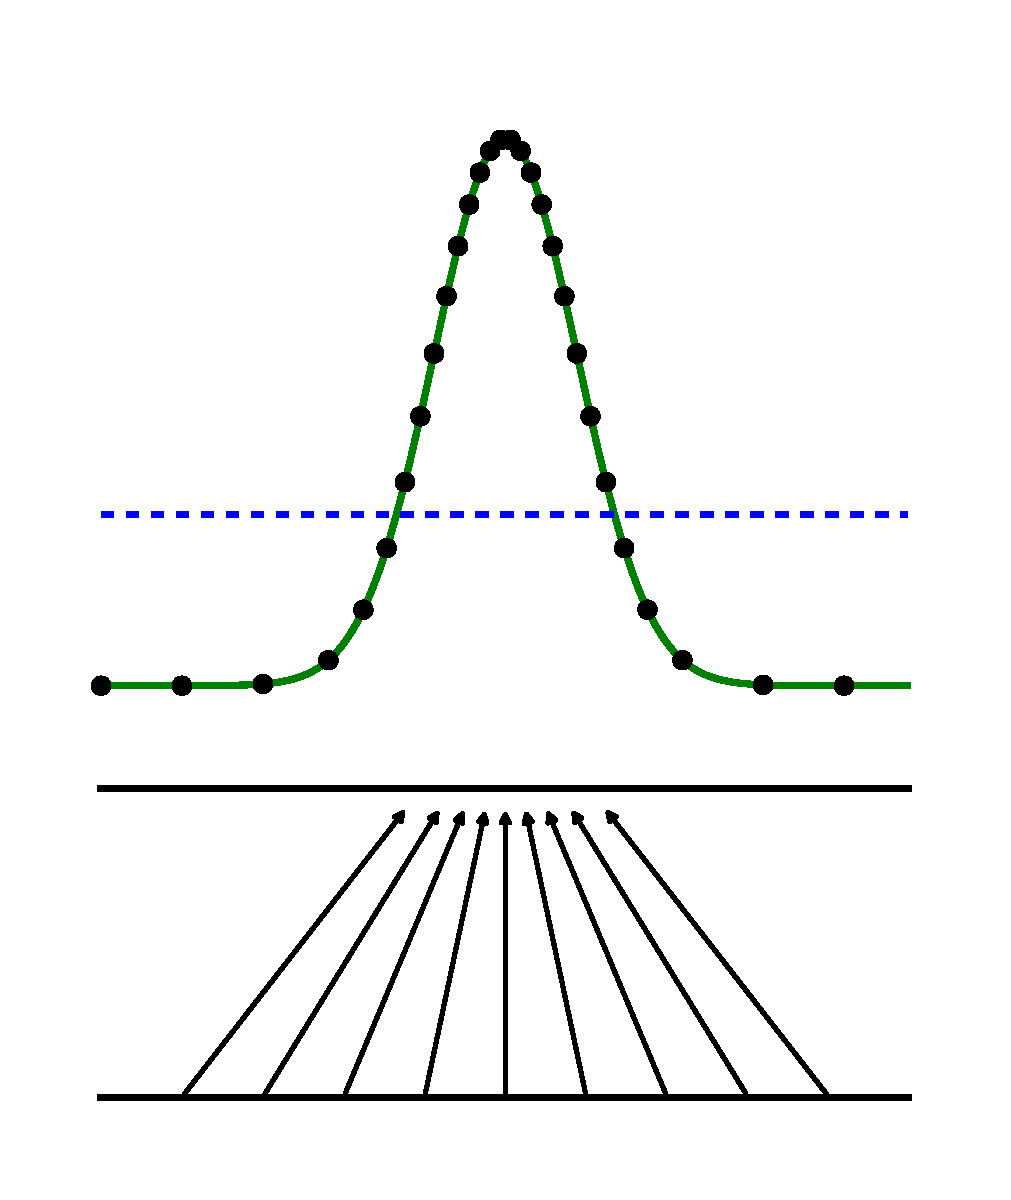
\includegraphics[width=0.9\textwidth]{figures/gan3.pdf}
            \caption{After}
        \end{figure}
    \end{minipage}

\end{frame}

% --- SLIDE 3 ---
\begin{frame}{Original GAN: Generation Examples}{Real vs generated comparisons}
    % Grid of generated samples 2x2 of MNIST, TFD, CIFAR and CIFAR with conv
    The right column shows the closest real samples to the generated ones on the left, illustrating that the model is not simply memorizing training data.\\
    \begin{minipage}[t]{0.48\textwidth}
        \begin{figure}
            \centering
            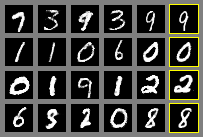
\includegraphics[width=0.5\textwidth]{figures/mnist_samples.png}
            \caption{MNIST samples}
        \end{figure}
    \end{minipage}
    \hfill
    \begin{minipage}[t]{0.48\textwidth}
        \begin{figure}
            \centering
            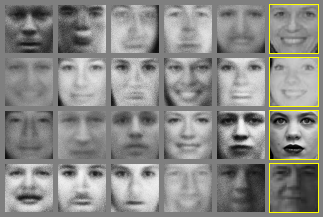
\includegraphics[width=0.5\textwidth]{figures/tfd_samples.png}
            \caption{Toronto Face Dataset samples}
        \end{figure}
    \end{minipage}
    \begin{minipage}[t]{0.48\textwidth}
        \begin{figure}
            \centering
            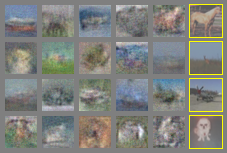
\includegraphics[width=0.5\textwidth]{figures/cifar_full_samples.png}
            \caption{CIFAR-10 samples (FC)}
        \end{figure}
    \end{minipage}
    \hfill
    \begin{minipage}[t]{0.48\textwidth}
        \begin{figure}
            \centering
            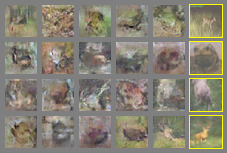
\includegraphics[width=0.5\textwidth]{figures/cifar_conv_samples.png}
            \caption{CIFAR-10 samples (ConvNet)}
        \end{figure}
    \end{minipage}
\end{frame}


\subsection{MNIST Generation}
\begin{frame}
    \begin{columns}[c, onlytextwidth]
        \column{0.5\textwidth}
        \centering $G$
        \begin{figure}
            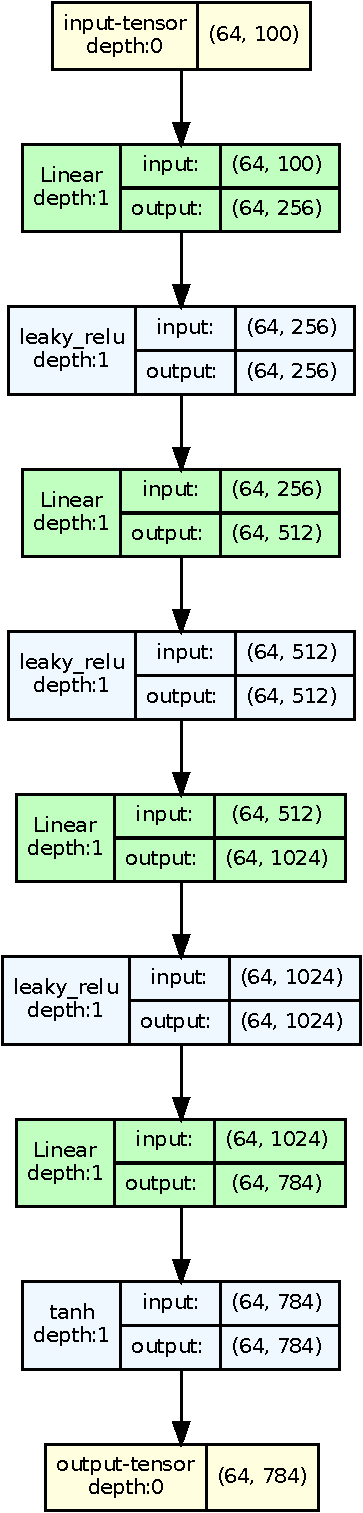
\includegraphics[width=0.2\textwidth]{figures/F.pdf}
        \end{figure}

        \column{0.5\textwidth}
        \centering $D$
        \begin{figure}
            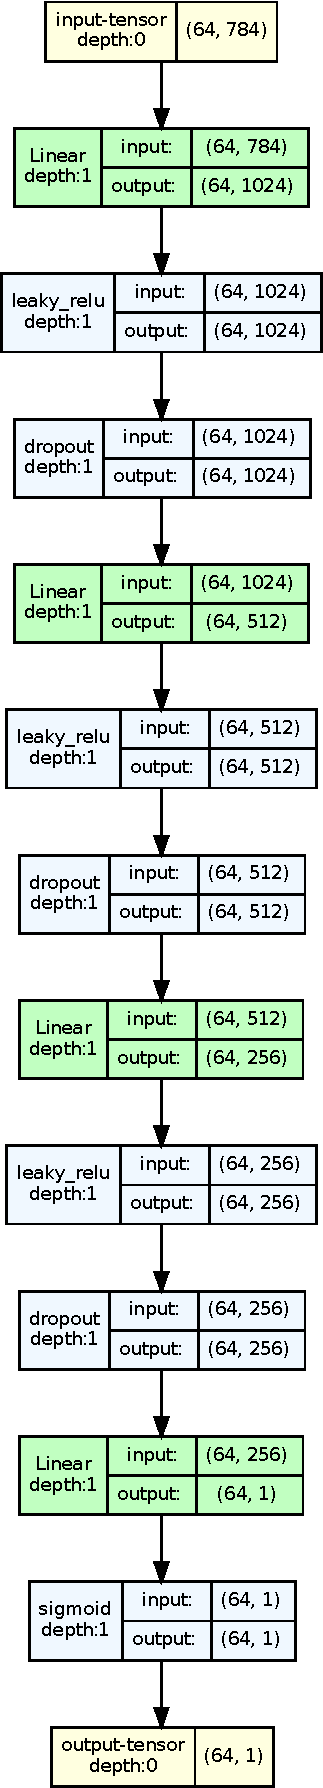
\includegraphics[width=0.2\textwidth]{figures/D.pdf}
        \end{figure}
    \end{columns}
\end{frame}

\begin{frame}
    \begin{figure}
        \centering
        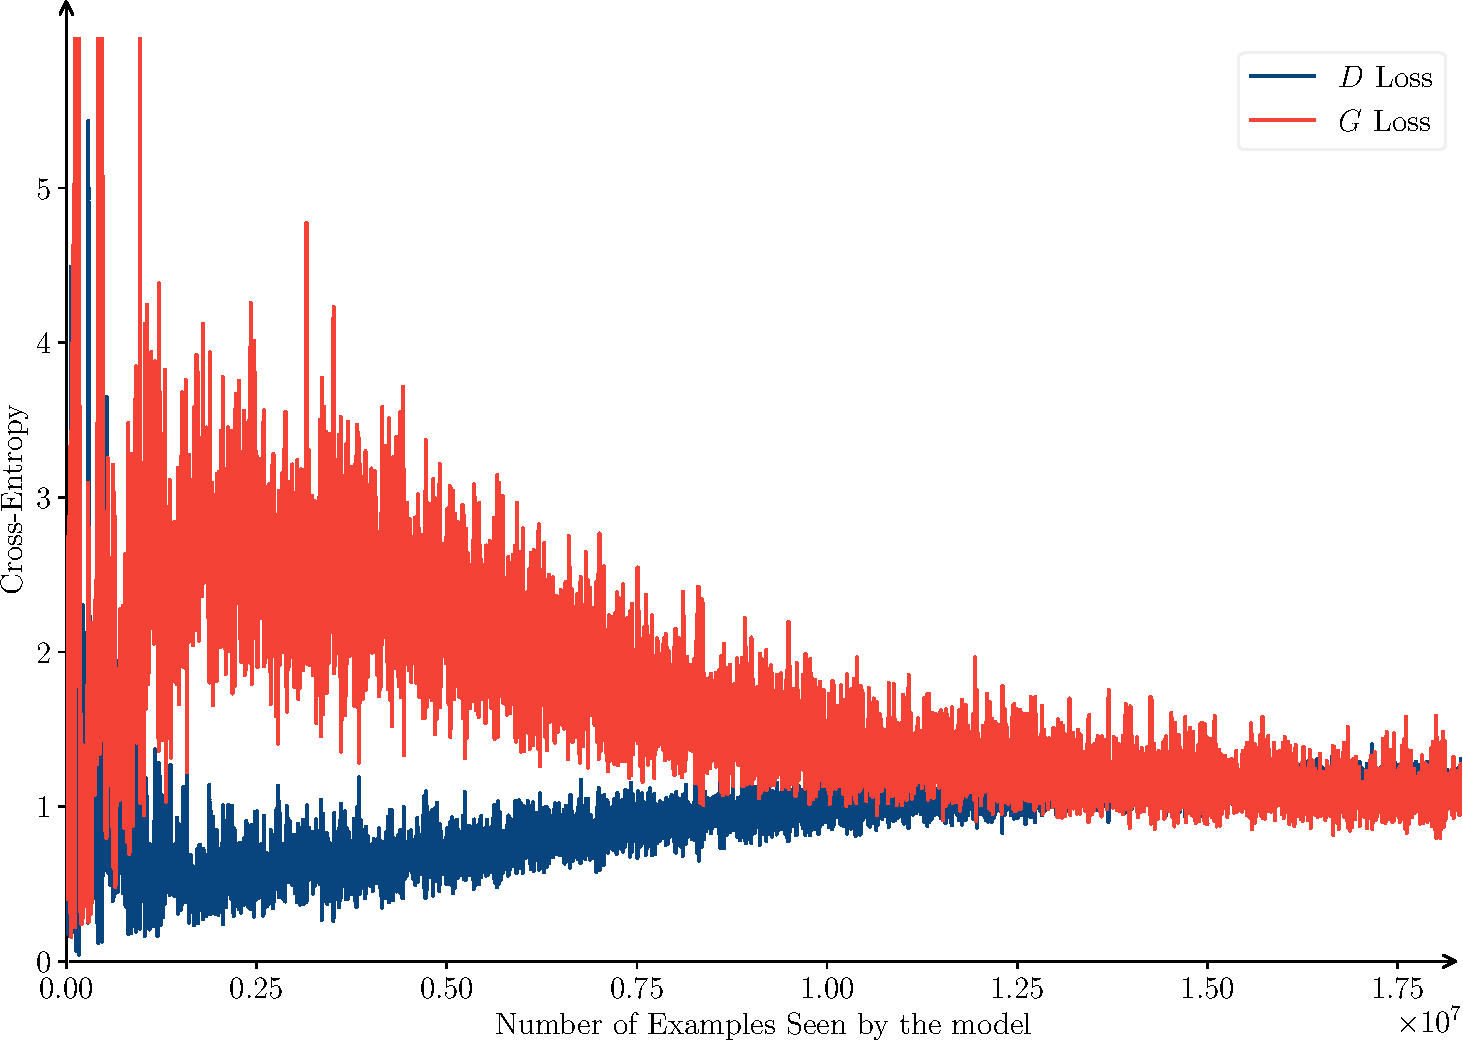
\includegraphics[width = 0.6 \textwidth]{figures/gan_loss.pdf}
    \end{figure}
\end{frame}

\begin{frame}
    \begin{figure}
        \animategraphics[autoplay,loop,width=0.4\textwidth]{15}{figures/GAN/sample_}{1}{305}
    \end{figure}
\end{frame}

% --- SLIDE 22 ---
\begin{frame}{Neural Architectures for GANs}{Why they matter \& milestones}
    \textbf{Why architectures matter}
    \begin{itemize}
        \item Stability of the adversarial game (gradient flow, Lipschitz control)
        \item Fidelity \& diversity of samples (texture, long-range structure)
        \item Scalability to high resolution and many classes
    \end{itemize}
    \vskip 6pt
    \textbf{Roadmap (milestones)}
    \begin{itemize}
        \item \textbf{2014} — Early GANs (MLPs; small images)
        \item \textbf{2015} — \emph{DCGAN}: conv/deconv stacks, BatchNorm, strided conv, (Leaky)ReLU
        \item \textbf{2017} — \emph{Progressive Growing}: fade-in layers for high-res synthesis
        \item \textbf{2018} — \emph{BigGAN}: class-conditional ResBlocks, self-attention, spectral norm
        \item \textbf{2018–2022} — \emph{StyleGAN → StyleGAN2 → StyleGAN-XL}: style modulation, noise injection, path-length reg
    \end{itemize}
    \vskip 4pt
    \textbf{Cross-cutting ideas}
    \begin{itemize}
        \item Normalization (BatchNorm in G/D; Spectral Norm in D)
        \item Conditioning (class embeddings, conditional BN)
        \item Architectural blocks (ResBlocks, attention) \& up/downsampling choices
    \end{itemize}

\end{frame}

% --- SLIDE 23 ---
\begin{frame}{Early GAN Architectures (MLP era)}{Template, limitations, takeaway}
    \textbf{Template (circa 2014)}
    \begin{itemize}
        \item \textbf{Generator $G$ (MLP):} $z\sim\mathcal N(0,I)\to$ dense layers $\to$ \texttt{tanh} output (image range $[-1,1]$)
        \item \textbf{Discriminator $D$ (MLP):} $x\to$ dense layers $\to$ sigmoid probability $D(x)\in(0,1)$
        \item Activations: ReLU/LeakyReLU in hidden layers; occasional Dropout; limited/no BN
        \item Target resolutions: small ($28\times28$, $32\times32$)
    \end{itemize}
    \vskip 6pt
    \textbf{Limitations observed}
    \begin{itemize}
        \item Poor inductive bias for images (no convolutions $\Rightarrow$ weak locality/translation handling)
        \item Training instability \& mode collapse at higher resolutions
        \item Limited long-range structure; textures often unrealistic
    \end{itemize}
    \vskip 4pt
    \textbf{Takeaway} \; Convolutional hierarchies (DCGAN) became the default to encode locality, share weights, and stabilize training.
\end{frame}

% --- SLIDE 24 ---
\begin{frame}{DCGAN}{Convolutional guidelines \& design choices}
    \textbf{Architecture guidelines for stable Deep Convolutional GANs (DCGAN) \citep{radford_unsupervised_2016}:}
    \begin{itemize}
        \item \textbf{Replace pooling} with \emph{strided convolutions} (discriminator) and \emph{fractional-strided convolutions} (generator).
        \item \textbf{Use BatchNorm} in both the generator and the discriminator.
        \item \textbf{Remove fully connected hidden layers} for deeper architectures.
        \item \textbf{Use ReLU in the generator} for all layers \textbf{except} the output, which uses \texttt{tanh}.
        \item \textbf{Use LeakyReLU in the discriminator} for \emph{all} layers.
    \end{itemize}
    \vskip 6pt
    \textit{Rationale:} encourage stable gradients, better conditioning, and convolutional inductive biases (locality, translation equivariance).
\end{frame}

% --- SLIDE 24.5 ---
\begin{frame}{DCGAN}{Architecture diagram \& rules of thumb}
    \begin{figure}
        \centering
        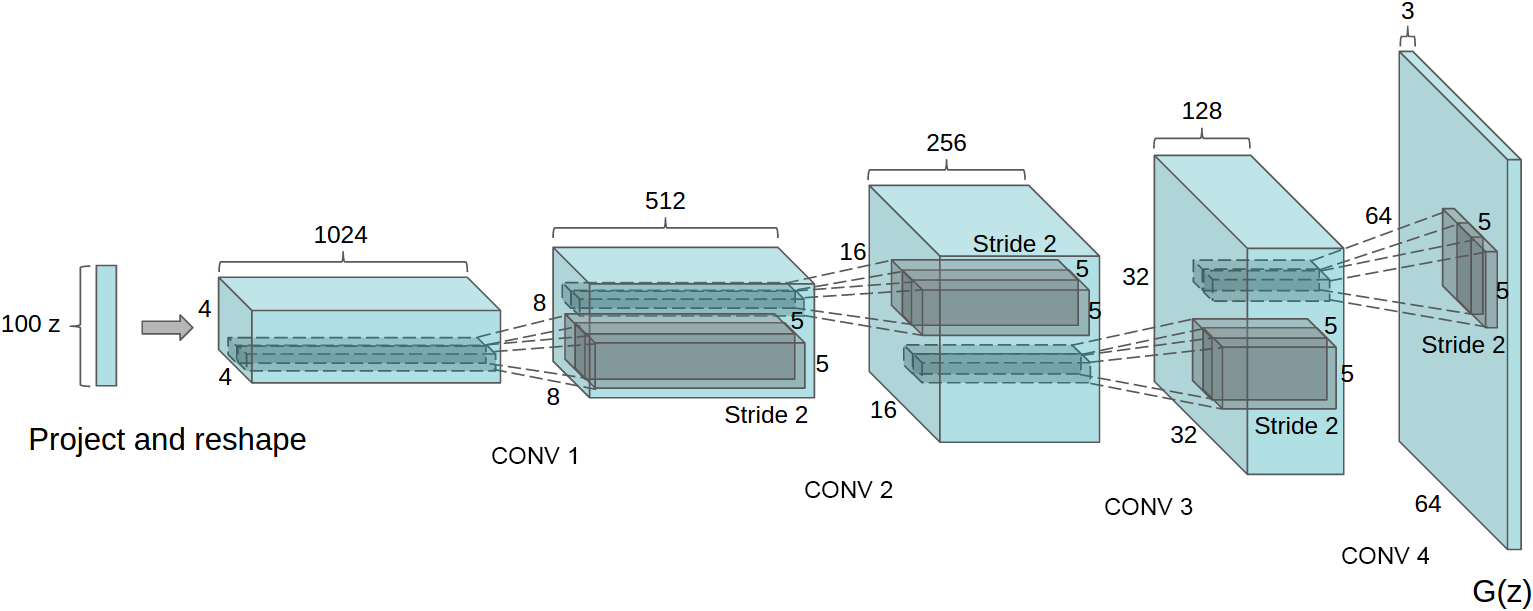
\includegraphics[width=0.8\textwidth]{figures/lsun_bedrooms_generator.png}
        \caption*{DCGAN architecture (Radford et al., 2015/2016).}
    \end{figure}
\end{frame}

% --- SLIDE 24.5.1 ---
\begin{frame}[t]{DCGAN}{Sample quality: MNIST \& faces}
    \only<1>{
        \begin{figure}
            \centering
            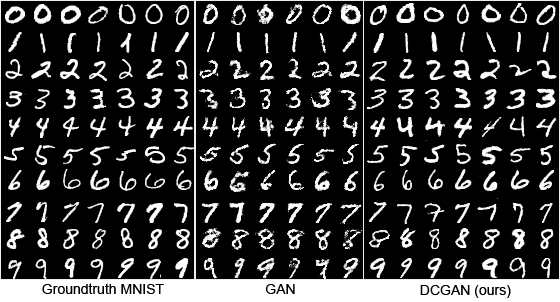
\includegraphics[width=0.9\linewidth]{figures/mnist_collage.png}
            \caption*{MNIST samples from DCGAN}
        \end{figure}
    }
    \only<2->{
        \begin{figure}
            \centering
            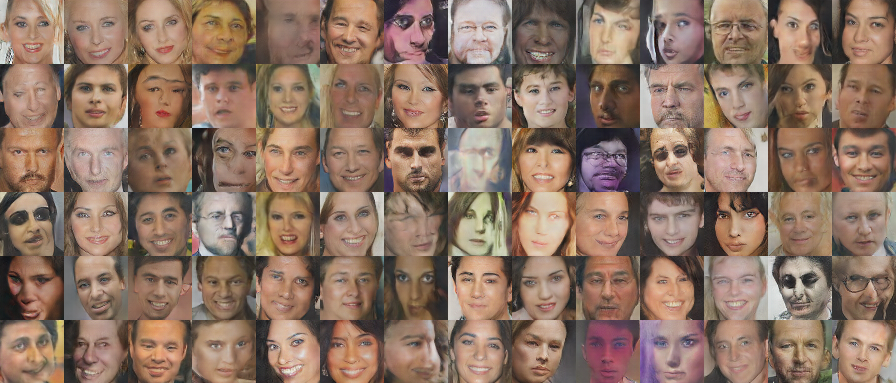
\includegraphics[width=0.6\linewidth]{figures/faces_128_filter_samples.png}
            \caption*{Faces (CelebA) from DCGAN}
        \end{figure}
        \only<3>{\textbf{Note:} quality improves markedly compared to early MLP GANs, but remains imperfect and at relatively low resolutions / latentdimensionalities. First decent generation in size 128x128}    }

\end{frame}

% --- SLIDE 25 ---
\begin{frame}{Progressive Growing of GANs}{Fade-in layers for high-resolution synthesis}
    \textbf{Key idea of \citet{karras_progressive_2018}:} progressively grow both the generator and discriminator during training.
    \begin{itemize}
        \item Train from low to high resolution (e.g., $4\times4\to8\times8\to\cdots\to1024\times1024$).
        \item \emph{Fade-in}: smoothly blend a newly added block over a transition period.
        \item Stabilizes training and improves high‑res detail; reduces compute at start.
        \item Generator: upsampling + conv blocks; Discriminator: mirror downsampling blocks.
    \end{itemize}
    \begin{figure}
        \centering
        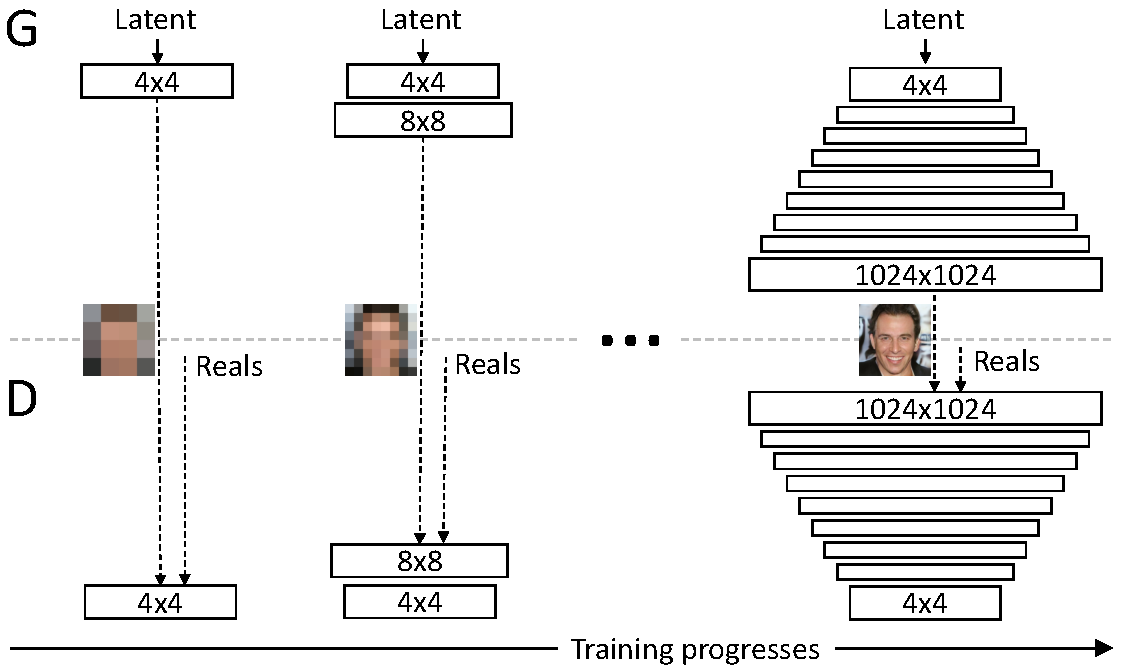
\includegraphics[width=0.5\linewidth]{figures/incremental.pdf}
        \caption*{Progressive growing architecture}
    \end{figure}
\end{frame}

% --- SLIDE 25.1 ---
\begin{frame}{Conditional Progressive Models}{Multi-scale super-resolution cascade}
    \begin{itemize}
        \item Conditional variants can be built as cascades of super‑resolution modules (e.g., $4\!\to\!8\!\to\!16\!\to\!\cdots$).
        \item Each stage upsamples and refines details conditioned on class/attributes.
        \item Useful for class‑conditional synthesis and guided upscaling.
    \end{itemize}
    \begin{figure}
        \centering
        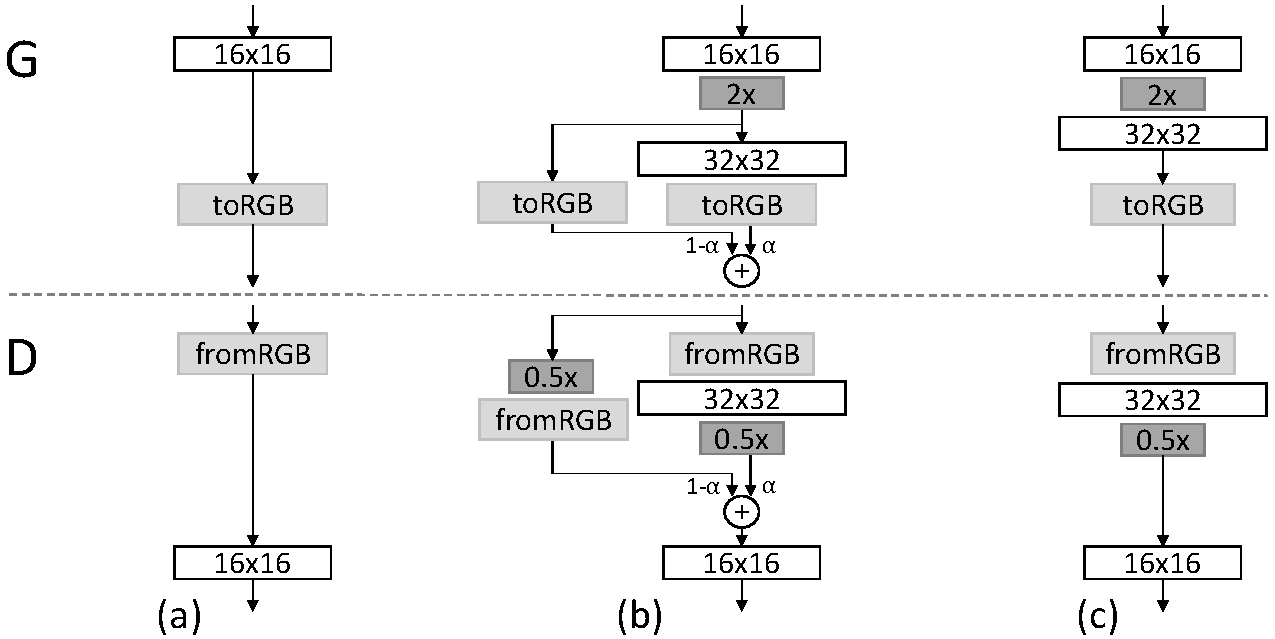
\includegraphics[width=0.6\linewidth]{figures/fadein.pdf}
        \caption*{Architectures of conditional super‑resolution models}
    \end{figure}
\end{frame}

% --- SLIDE 25.2 ---
\begin{frame}{Progressive Growing: Training Cost}{Time vs image size}
    \begin{figure}
        \centering
        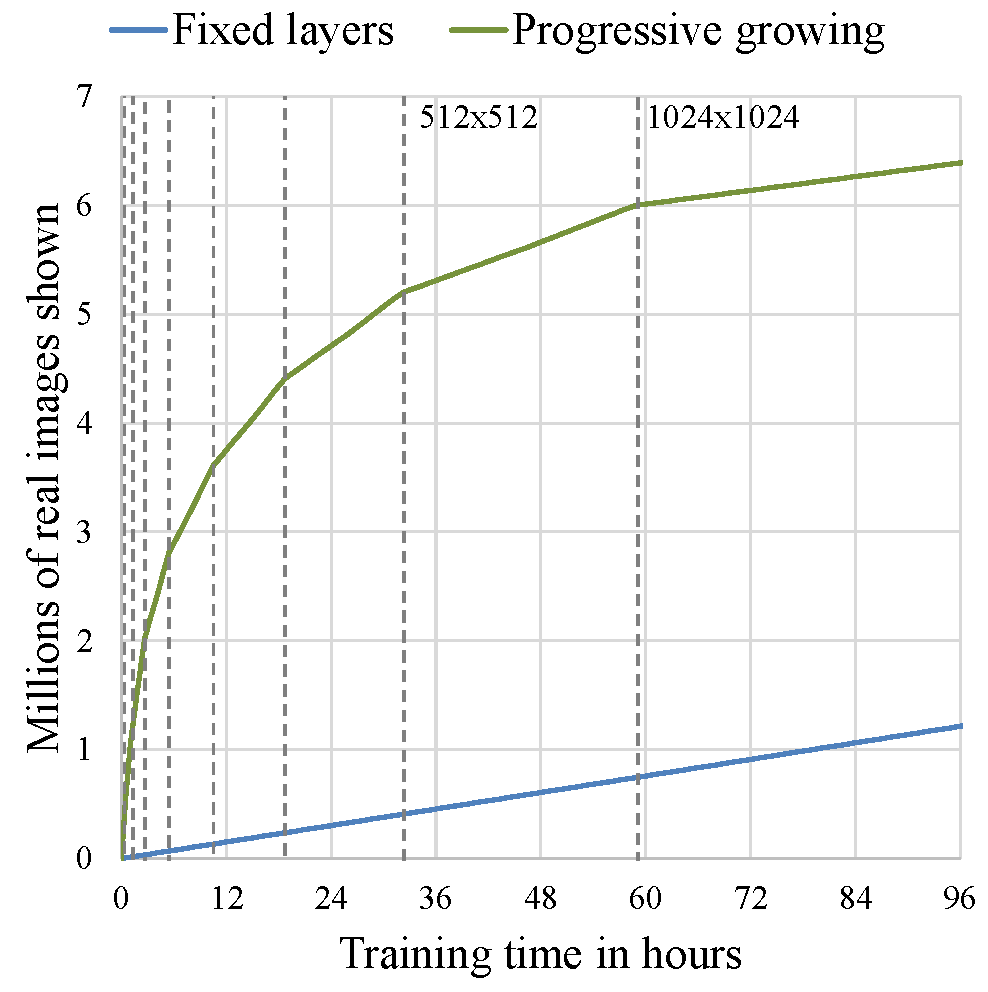
\includegraphics[width=0.5\linewidth]{figures/plot-perf-fixed-vs-grow2.pdf}
        \caption*{Training time as a function of image size}
    \end{figure}
    \textbf{Note:} early phases are cheap (small grids), heavy compute spent only at high resolutions.
\end{frame}

% --- SLIDE 25.3 ---
\begin{frame}{PGGAN Samples}{CelebA, LSUN}
    \only<1>{
        \textbf{Note:} PGGAN produces high-quality, high-resolution samples (1024x1024) with good global structure and fine details.
        \begin{figure}
            \centering
            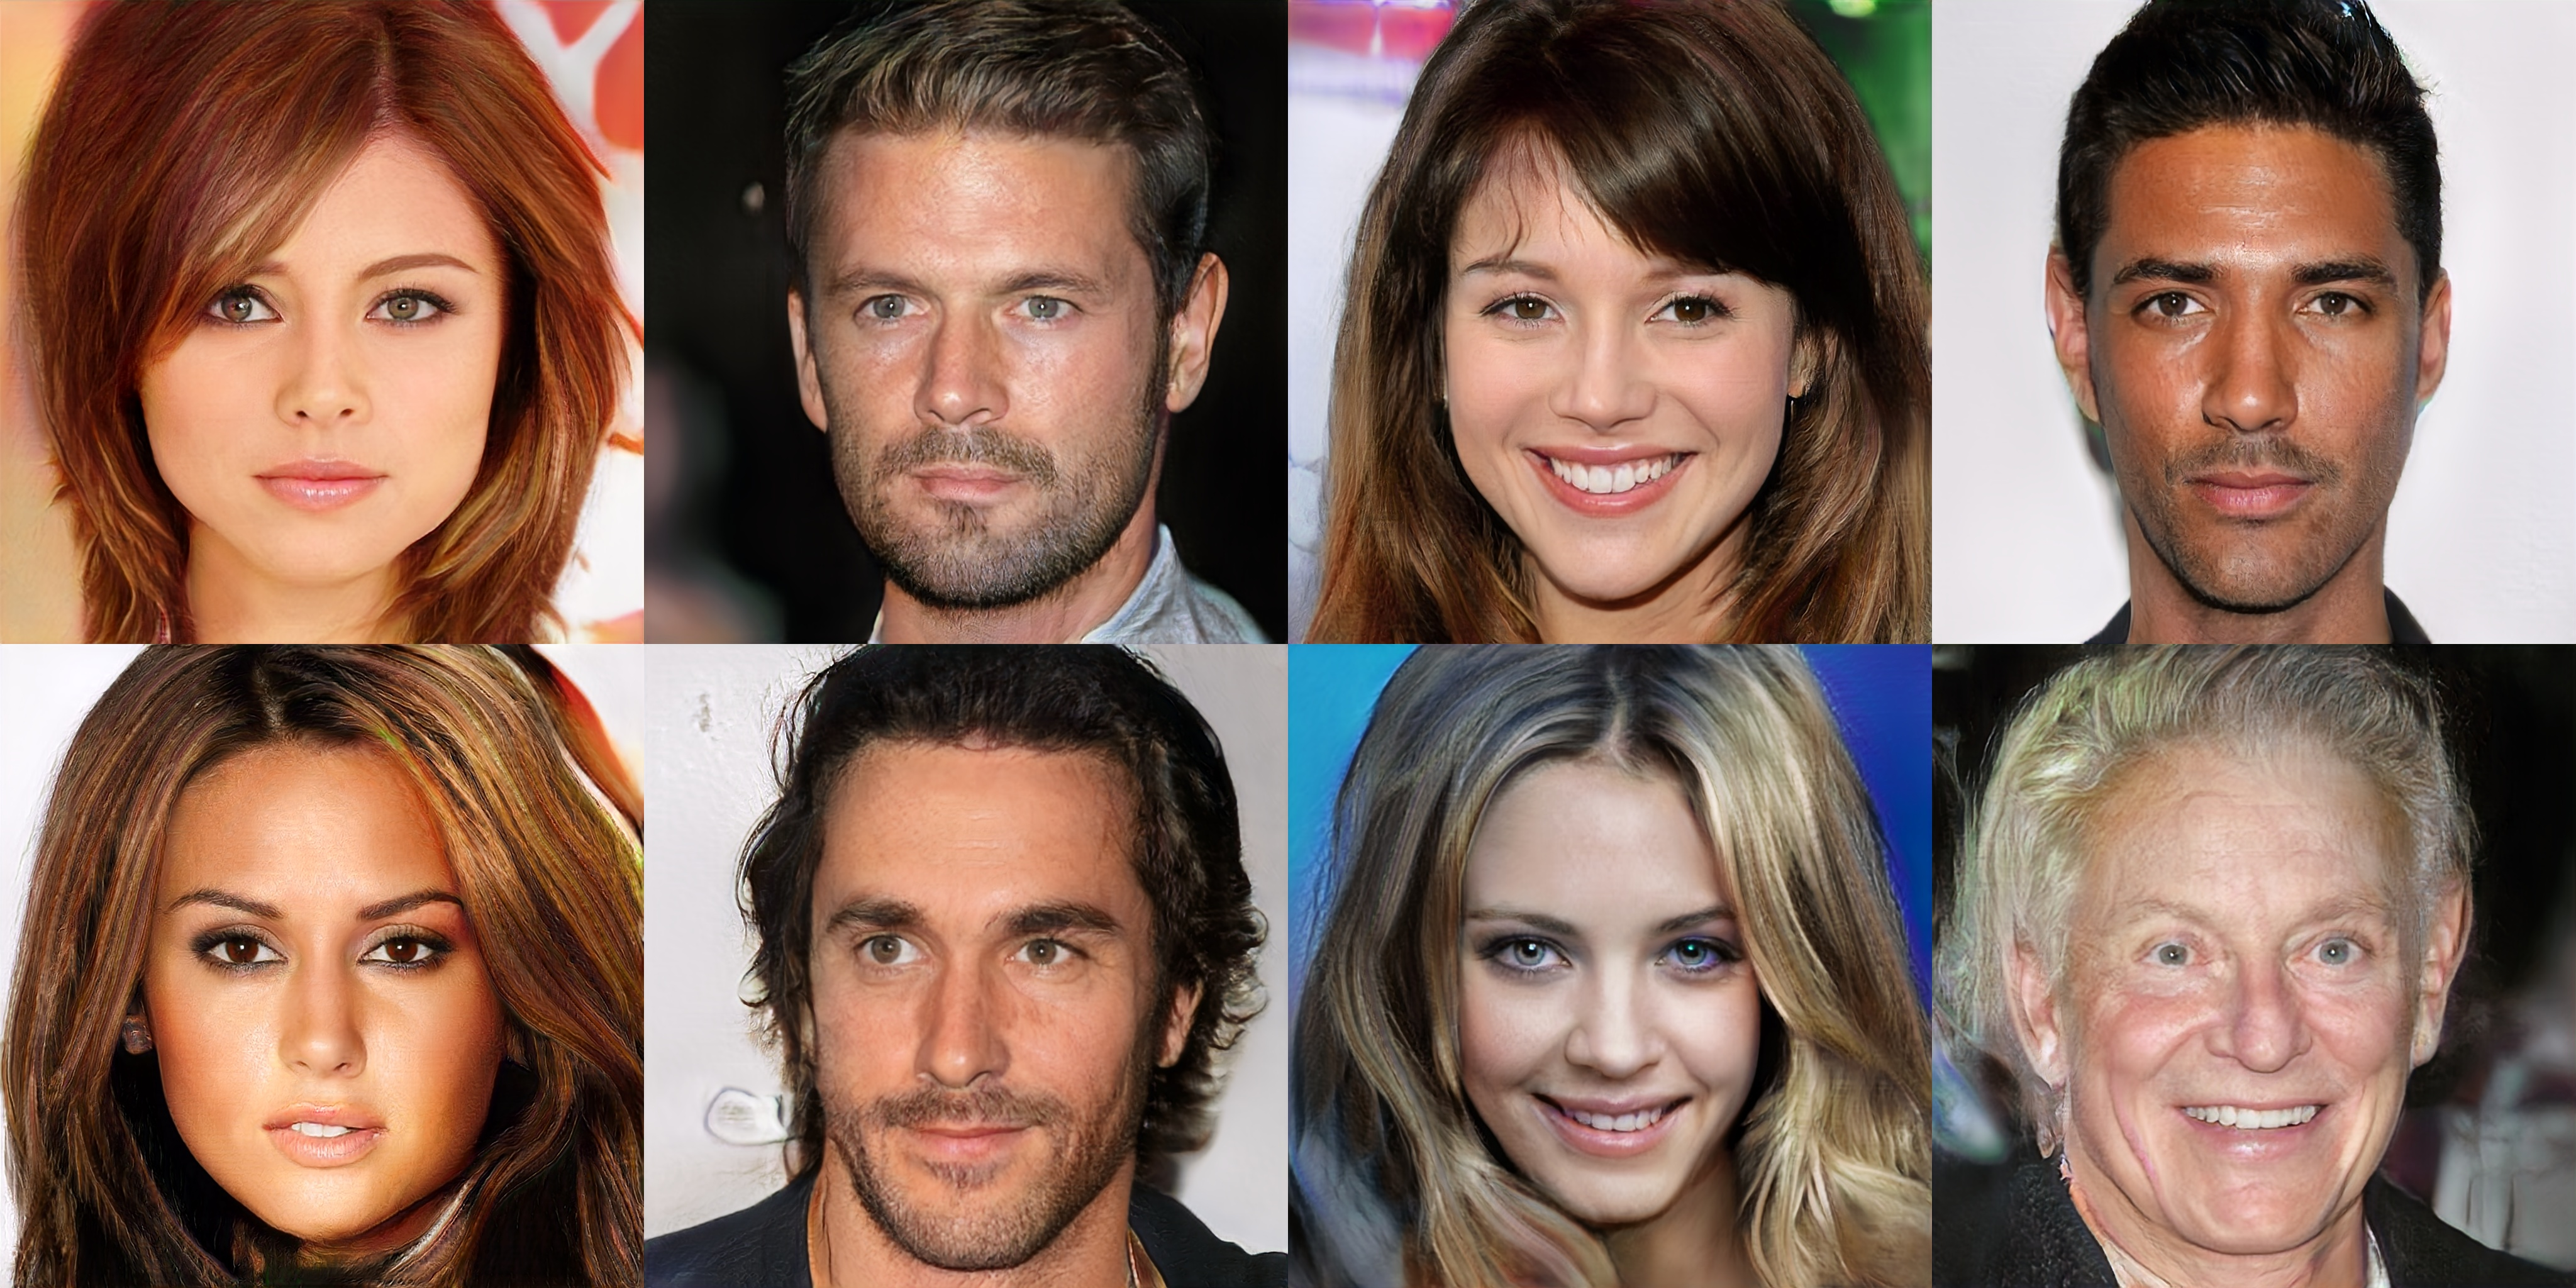
\includegraphics[width=0.95\linewidth]{figures/celeb1024-results.jpg}
            \caption*{CelebA}
        \end{figure}
    }
    \only<2-6>{
        LSUN dataset contains large-scale scene categories (bedrooms, churches, etc.) with diverse layouts and objects.
        \begin{figure}
            \centering
            \only<2>{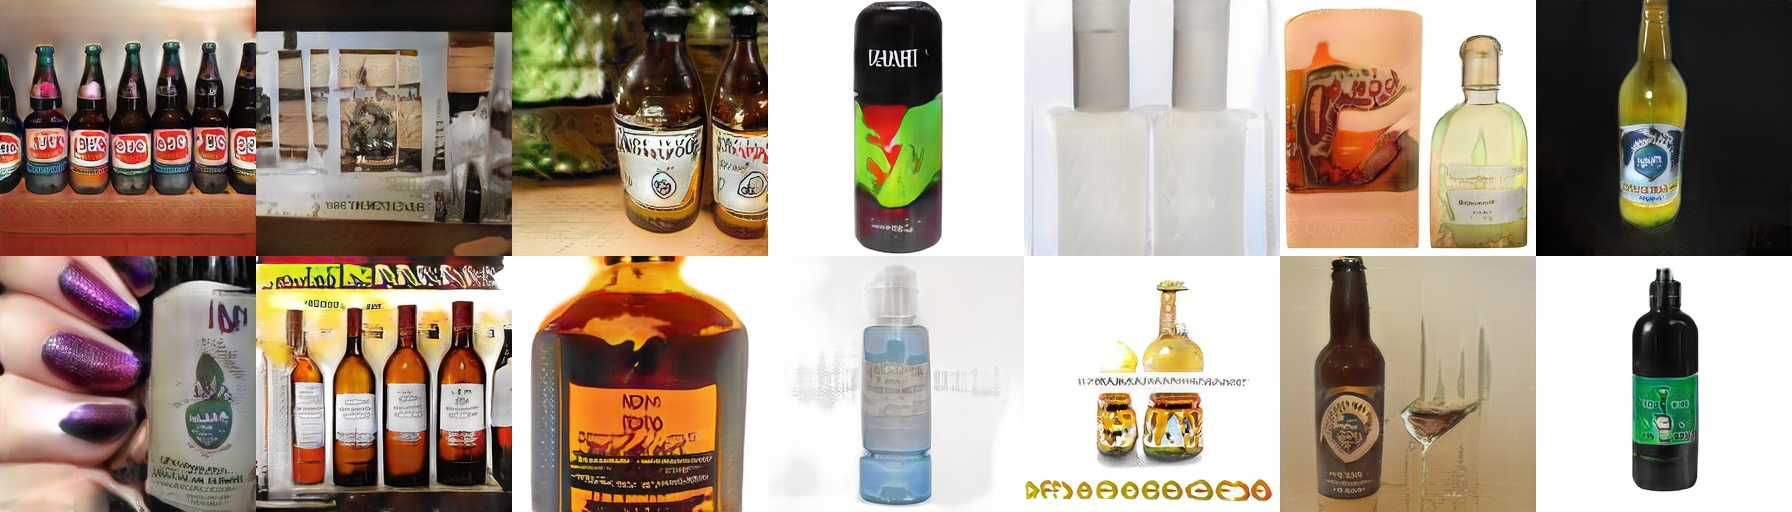
\includegraphics[width=0.95\linewidth]{figures/LSUNbottle.jpg}}
            \only<3>{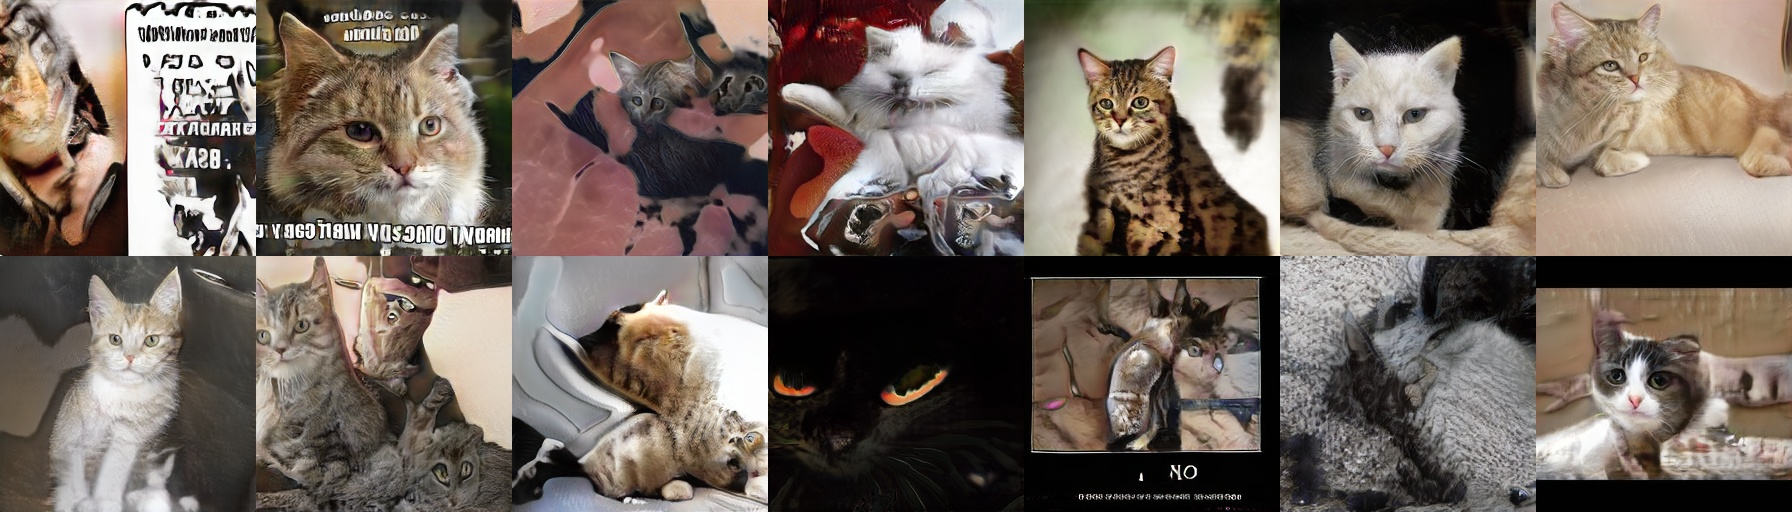
\includegraphics[width=0.95\linewidth]{figures/LSUNcat.jpg}}
            \only<4>{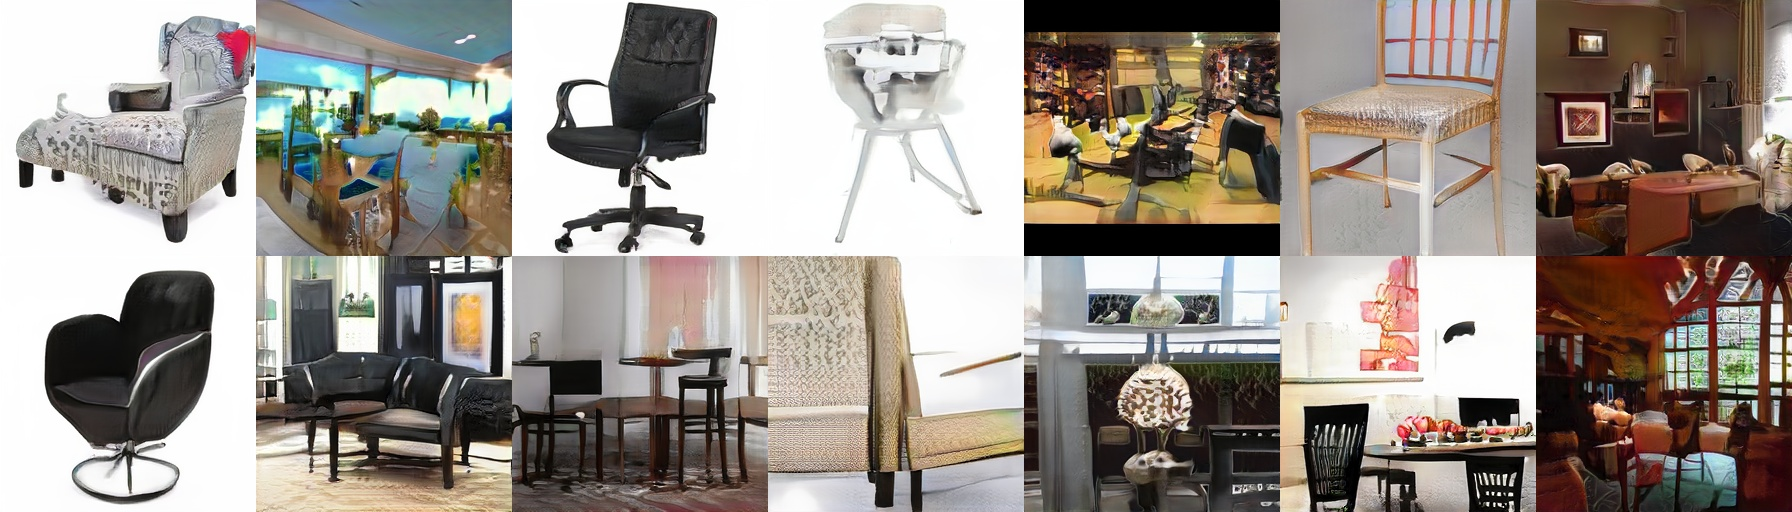
\includegraphics[width=0.95\linewidth]{figures/LSUNchair.jpg}}
            \only<5>{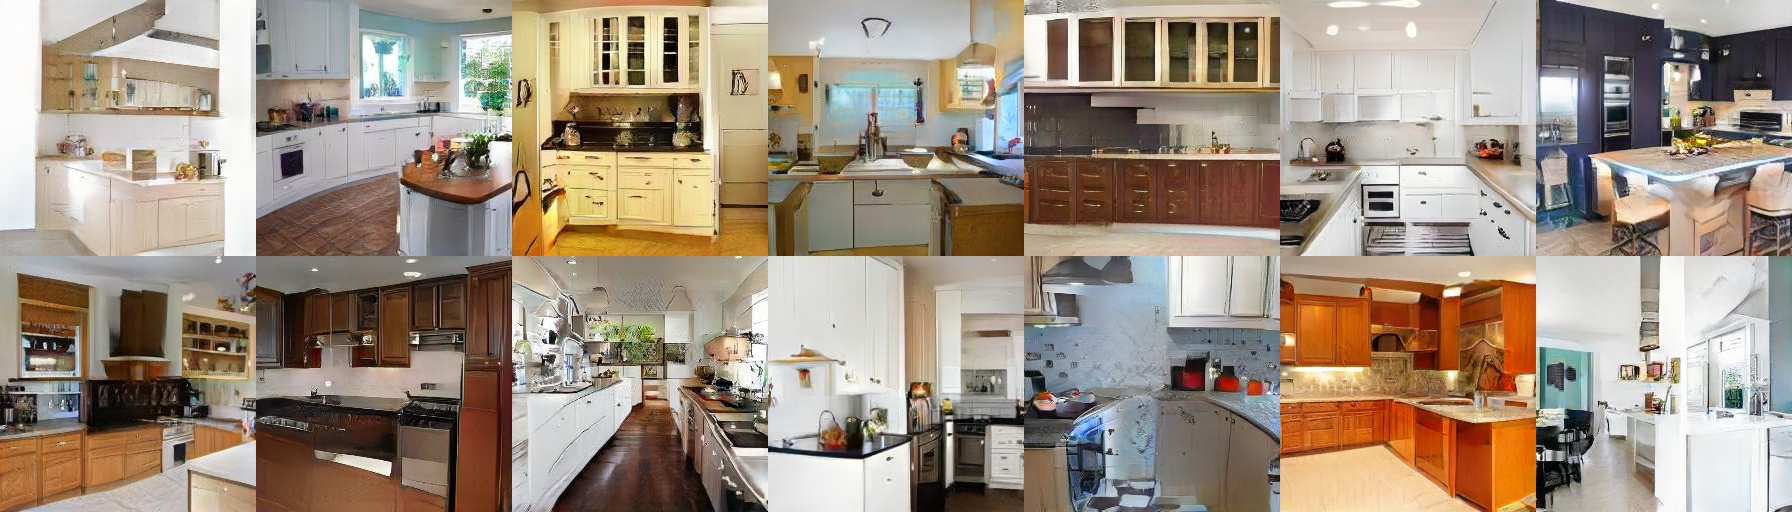
\includegraphics[width=0.95\linewidth]{figures/LSUNkitchen.jpg}}
            \only<6>{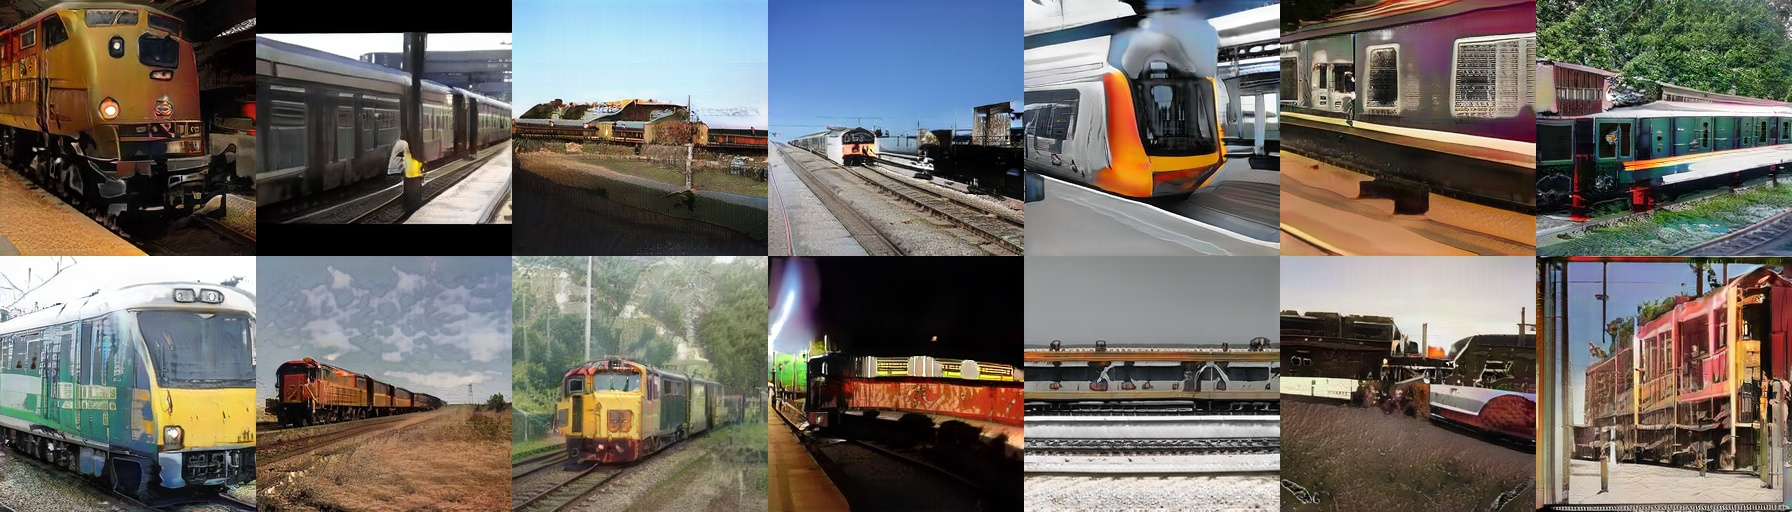
\includegraphics[width=0.95\linewidth]{figures/LSUNtrain.jpg}}
            \caption*{LSUN}
        \end{figure}
    }
\end{frame}

\vspace{0.5em}
% --- SLIDE 26 ---
\begin{frame}{BigGAN}{Class-conditional, attention, spectral norm}
    \textbf{Key improvements \citet{brock_large_2019}:}
    \begin{itemize}
        \item \textbf{Class-conditional architecture:} shared class embeddings + \emph{conditional BatchNorm} in $G$; deep residual blocks.
        \item \textbf{Long-range modeling:} non-local \emph{self-attention} layers (SAGAN-style) to capture global structure.
        \item \textbf{Stability \& fidelity:} \emph{spectral normalization} in $D$ \emph{and} $G$, very large-batch training, and the \emph{truncation trick} (trade-off between FID and diversity).
    \end{itemize}
    \begin{figure}
        \centering
        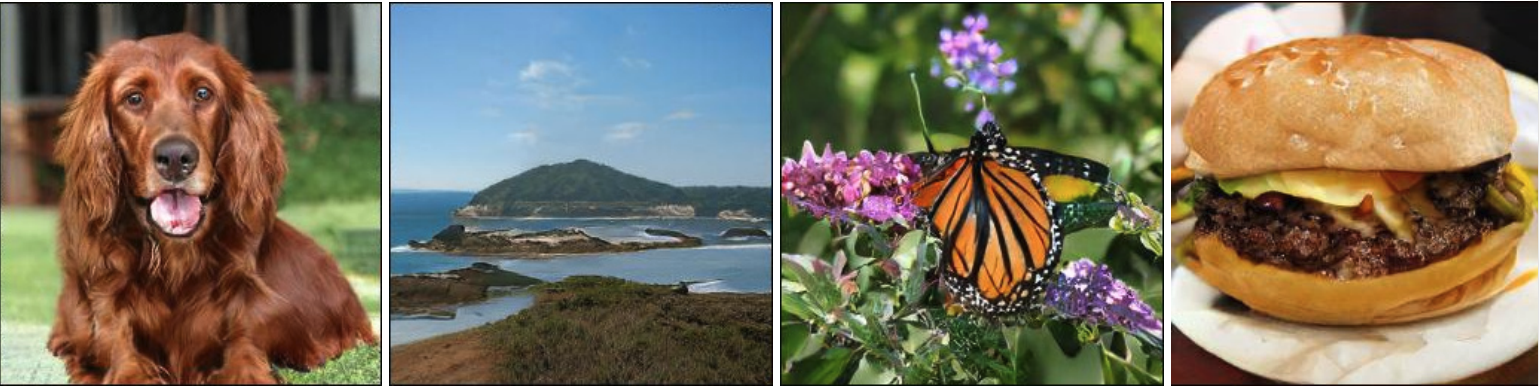
\includegraphics[width=0.7\linewidth]{figures/biggan.png}
        \caption*{BigGAN: class-conditional + attention + SN}
    \end{figure}
\end{frame}

% --- SLIDE 27 ---
\begin{frame}{StyleGAN \& StyleGAN-XL}{Style modulation, noise, path length reg}
    \textbf{Three milestones}
    \begin{itemize}
        \item \textbf{StyleGAN (2019):} style-based generator with mapping network; \emph{style modulation} (AdaIN) per layer; per-pixel noise for stochastic detail; improved disentanglement. \;(\citet{karras_style-based_2019})
        \item \textbf{StyleGAN2 (2020):} removes AdaIN artifacts via \emph{weight demodulation}; \emph{path length regularization}; architectural refinements for higher fidelity and fewer texture droplet artifacts. \;(\citet{karras_analyzing_2020})
        \item \textbf{StyleGAN-XL (2022):} scales StyleGAN to large, diverse datasets (e.g., ImageNet); stronger conditioning and training tricks; state-of-the-art FID/IS at higher resolutions. \;(\citet{sauer_stylegan-xl_2022})
    \end{itemize}
    \vskip 4pt
    Example of realism: \href{https://thispersondoesnotexist.com}{ThisPersonDoesNotExist.com} (StyleGAN faces).

\end{frame}

% --- SLIDE 28 ---
\begin{frame}{Domain Adaptation with GANs}{Motivation \& setup}
    \begin{itemize}
        \item \textbf{Goal:} translate from a \emph{source} domain $X$ to a \emph{target} domain $Y$ \emph{without} paired examples (unpaired domain adaptation).
        \item \textbf{Challenge:} many valid mappings $X\to Y$; need additional structure to avoid degenerate solutions.
        \item \textbf{Key idea:} use \emph{consistency losses} (cycle/identity) to regularize adversarial training.
    \end{itemize}
    \vskip 6pt
    \begin{figure}
        \centering
        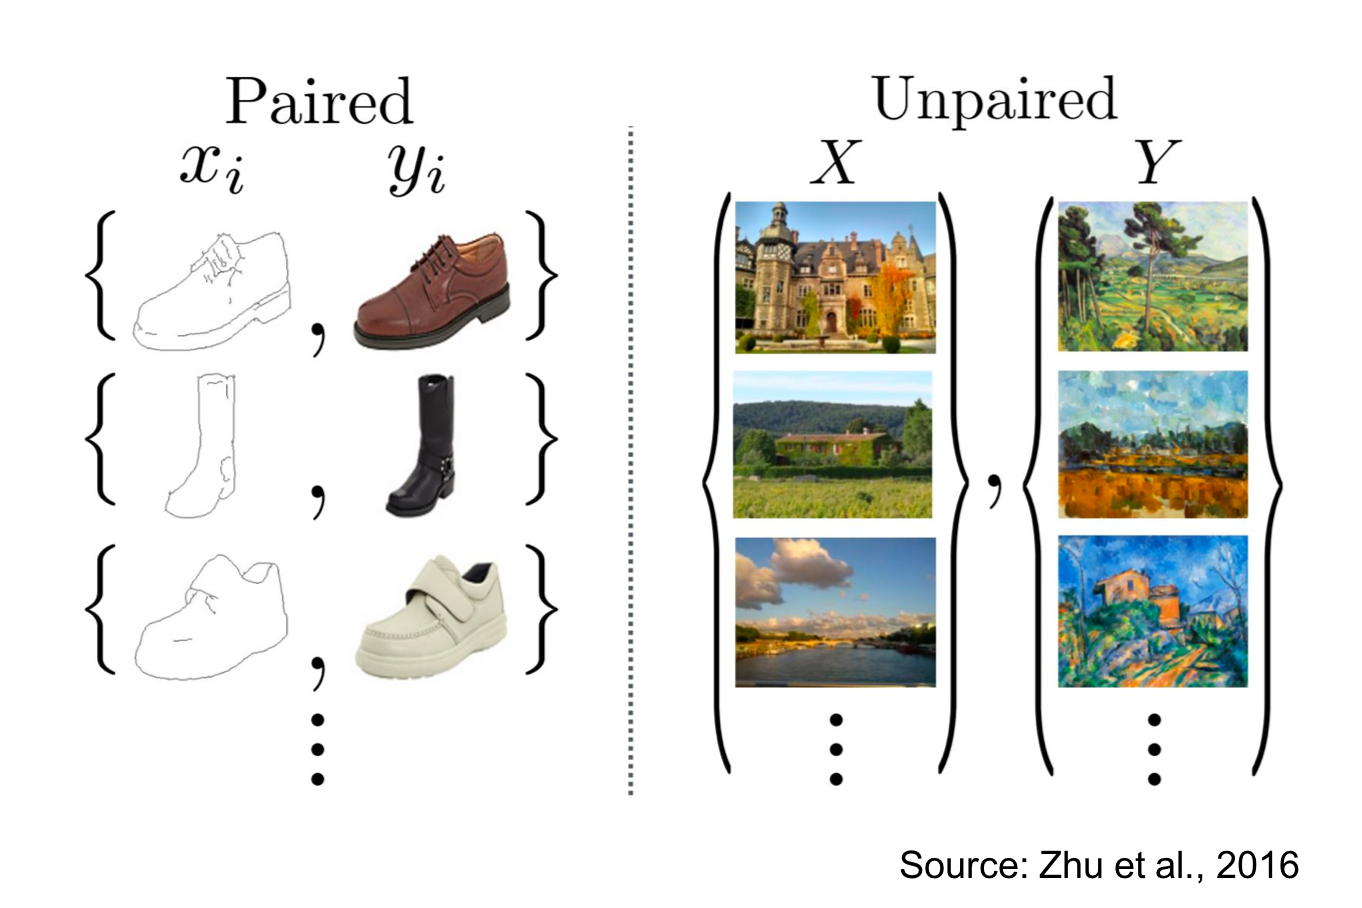
\includegraphics[width=0.6\linewidth]{figures/6.png}
        \caption*{Supervision regimes for domain adaptation}
    \end{figure}
\end{frame}

% --- SLIDE 29 ---
\begin{frame}{CycleGAN: Model}{Two generators, two discriminators}
    Let $G: X\to Y$ and $F: Y\to X$ with discriminators $D_Y$ and $D_X$.
    \begin{align*}
        \mathcal L_{\mathrm{GAN}}(G,D_Y) & = \E_{y\sim p_Y}[\log D_Y(y)] + \E_{x\sim p_X}[\log (1 - D_Y(G(x)))], \\
        \mathcal L_{\mathrm{GAN}}(F,D_X) & = \E_{x\sim p_X}[\log D_X(x)] + \E_{y\sim p_Y}[\log (1 - D_X(F(y)))].
    \end{align*}
    \vskip 4pt
    \begin{figure}
        \centering
        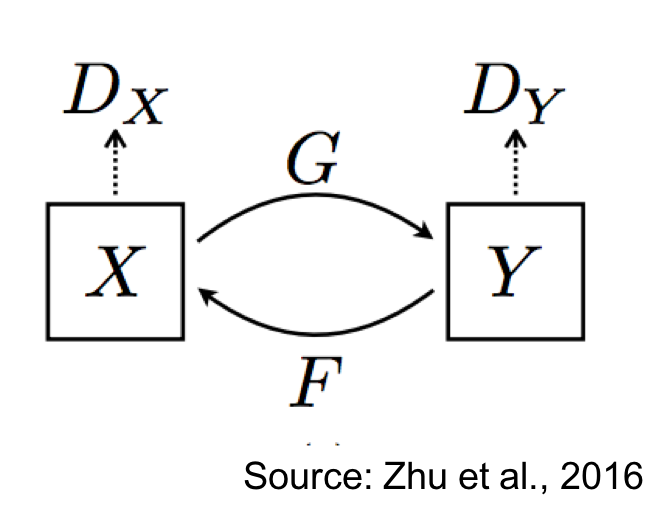
\includegraphics[width=0.5\linewidth]{figures/7.png}
        \caption*{Adversarial setup (two directions)}
    \end{figure}
\end{frame}

% --- SLIDE 30 ---
\begin{frame}{CycleGAN: Consistency Losses}{Why unpaired translation works}
    \textbf{Cycle-consistency:}
    \begin{equation*}
        \mathcal L_{\mathrm{cyc}}(G,F) = \E_{x\sim p_X}\big[\,\|F(G(x)) - x\|_1\,\big] + \E_{y\sim p_Y}\big[\,\|G(F(y)) - y\|_1\,\big].
    \end{equation*}

    \textbf{Total objective:}
    \begin{equation*}
        \min_{G,F}\max_{D_X,D_Y} \; \mathcal L_{\mathrm{GAN}}(G,D_Y)+\mathcal L_{\mathrm{GAN}}(F,D_X) + \lambda_\mathrm{cyc}\,\mathcal L_{\mathrm{cyc}} .
    \end{equation*}
    \vskip 4pt
    \begin{figure}
        \centering
        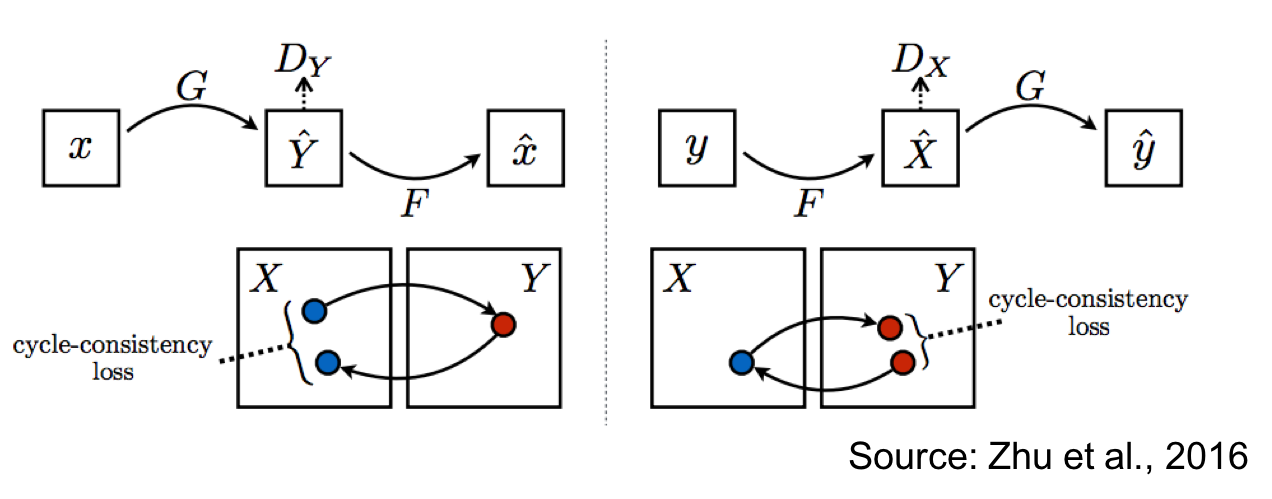
\includegraphics[width=0.75\linewidth]{figures/8.png}
        \caption*{Consistency regularization}
    \end{figure}
\end{frame}

% --- SLIDE 31 ---
\begin{frame}{CycleGAN: Qualitative Results}{Monet\,$\leftrightarrow$\,Photo; Horse\,$\leftrightarrow$\,Zebra; Summer\,$\leftrightarrow$\,Winter}
    \begin{figure}
        \centering
        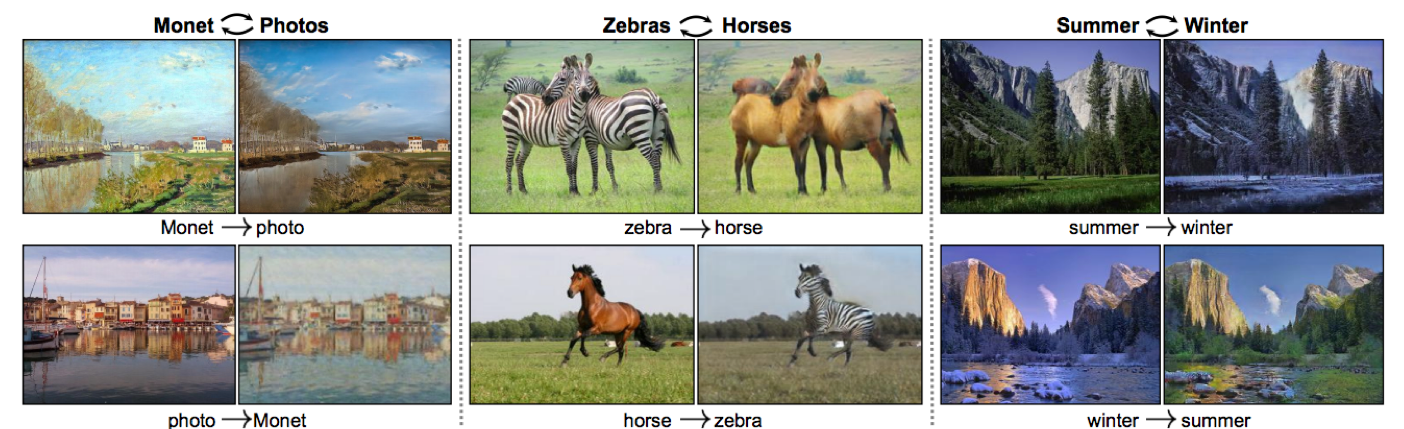
\includegraphics[width=0.8\linewidth]{figures/9.png}
        \caption*{Unpaired image-to-image translation}
    \end{figure}
\end{frame}

% --- SLIDE 31.5 ---
\begin{frame}{CycleGAN: Qualitative Results}{Photography\,$\leftrightarrow$\,Monet, Cezanne, Van Gogh, Ukiyo-e}
    \begin{figure}
        \centering
        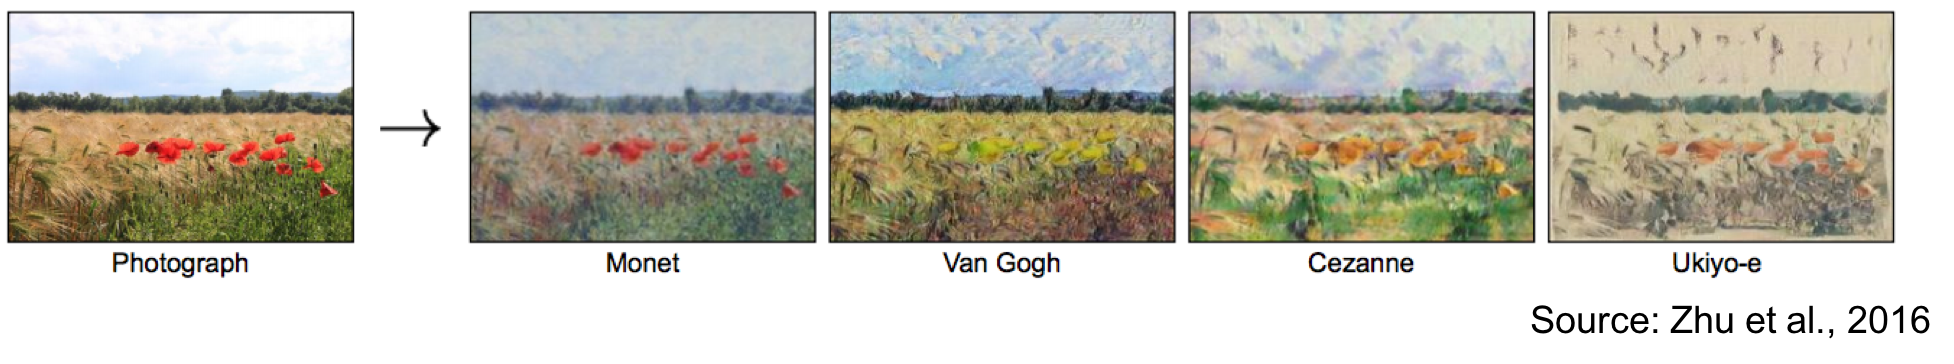
\includegraphics[width=0.8\linewidth]{figures/10.png}
        \caption*{Unpaired image-to-image translation}
    \end{figure}
\end{frame}

\begin{frame}{}{Your turn !}
    Get the Notebook on the course website and start working on it.
    \begin{itemize}
        \item \url{https://www.alexverine.com}
        \item Teaching
        \item Introduction to Deep Learning
        \item Lien Notebook
    \end{itemize}
    During this hands-on session we will train a GAN first on two dimensional data, and then on the MNIST dataset. Don't hesitate to use Colab or your own computer to run the notebook.
\end{frame}


% \begin{frame}[allowframebreaks]{References}
%     \printbibliography
% \end{frame}
\end{document}
